\documentclass[12pt, a4paper]{report}
\usepackage{hyperref}
\usepackage[top=3cm,right=3cm,bottom=3cm,left=2.5cm]{geometry}
\usepackage{caption}
\usepackage{indentfirst}
\usepackage{graphicx}
\usepackage{subfigure}
\usepackage{float}
\usepackage{amsmath}
\usepackage{listings} % Load the listings package
\usepackage{xcolor}   % Optional: For custom colors
\usepackage{longtable}
\usepackage{array}
\usepackage{tikz}
\usetikzlibrary{shapes.geometric, arrows.meta} % Use arrows.meta library
\usepackage{fancyhdr}
\usepackage{pdfpages}
\usepackage{amsmath, amssymb, amsfonts}
\usepackage{booktabs}
\usepackage{needspace}

\usepackage{hyperref}


\usepackage{xepersian}
\settextfont{B Nazanin}
\linespread{1.2}
\setcounter{secnumdepth}{2}
\setcounter{tocdepth}{2}

\tikzstyle{startstop} = [rectangle, rounded corners, minimum width=3cm,
                         minimum height=1cm,text centered, draw=black, fill=red!30]

\tikzstyle{process} = [rectangle, minimum width=3cm, minimum height=1cm,
                       text centered, draw=black, fill=blue!30]

\tikzstyle{arrow} = [thick,->,>=stealth]


\pagestyle{fancy}
% Set up fancyhdr to place page number at the top left
\pagestyle{fancy}
\fancyhf{} % Clear all header/footer fields
\fancyhead[L]{\thepage} % Page number on the top left

% Define custom style for chapter page (no header or footer)
\fancypagestyle{plain}{
	\fancyhf{} % Clear headers and footers
	\renewcommand{\headrulewidth}{0pt} % Remove header rule
}


% Changing TOC addressing format (from period separation to dash seperation)
\renewcommand{\thesection}{\thechapter-\arabic{section}-}
\renewcommand{\thesubsection}{\thechapter-\arabic{section}-\arabic{subsection}-}
\renewcommand{\thesubsubsection}{\thechapter-\arabic{section}-\arabic{subsection}-\arabic{subsubsection}-}

\renewcommand{\thetable}{(\thechapter-\arabic{table})}

% Redefine how captions are written 
\renewcommand{\thefigure}{(\thechapter-\arabic{figure})}

% Set caption font size to 11pt
\captionsetup{font=small, labelsep=space} % 'small' is equivalent to 11pt in most classes

% Make sure Persian and Latin text have their respective font sizes
\settextfont{B Nazanin} % Persian font
\setlatintextfont{Times New Roman} % Latin font

% Automatically switch between Persian and Latin fonts based on character type
\XeTeXinterchartokenstate=1
\newXeTeXintercharclass\persianchars
\newXeTeXintercharclass\latinchars

% Automatically switch fonts when switching between Persian and Latin characters
\XeTeXinterchartoks \latinchars \persianchars = {\begingroup\persianfont\endgroup}
\XeTeXinterchartoks \persianchars \latinchars = {\begingroup\latinfont\endgroup}



\title{گزارش کارآموزی}
\author{متین اعظمی}

\begin{document}

\begin{titlepage}
    \centering
    % University logo
    
\includegraphics[width=0.25\textwidth]{photos/university-logo.png}\par\vspace{1cm}
    
    % University and Faculty name
    {\Large دانشگاه اصفهان}\par
    {\large دانشکده مهندسی کامپیوتر}\par
    {\large گروه هوش مصنوعی}\par
    \vspace{1.5cm}
    
    % Report title
    {\bfseries\LARGE گزارش پروژه کارشناسی}\par\vspace{1cm}
    {\large \textbf{رشته مهندسی کامپیوتر گرایش هوش مصنوعی}}\par\vspace{1.2cm}
    
    {\large {عنوان پروژه:}}\par\vspace{0.5cm}
    {\Large \textbf{توسعه يك عامل يادگيري تقويتي براي تصميم‌گيري در بازارهاي مالي با بهره‌گيري از مدل‌هاي زباني بزرگ}}\par\vspace{1.5cm}
    
    {\large {استاد راهنما:}}\par\vspace{0.3cm}
    {\large \textbf{دکتر حسین کارشناس}}\par\vspace{1.2cm}
    
    {\large {پژوهشگر:}}\par\vspace{0.3cm}
    {\large \textbf{متین اعظمی}}\par\vspace{1.2cm}
    
    {\large شهریور ۱۴۰۴}\par
\end{titlepage}
	

\begin{titlepage}
    \centering
    % University logo
    
\includegraphics[width=0.25\textwidth]{photos/university-logo.png}\par\vspace{1cm}
    
    % University and Faculty name
    {\Large دانشگاه اصفهان}\par
    {\large دانشکده مهندسی کامپیوتر}\par
    {\large گروه هوش مصنوعی}\par
    \vspace{1.5cm}
    
    % Report title
    {\bfseries\LARGE پروژه کارشناسی رشته مهندسی کامپیوتر گرایش هوش مصنوعی}\par\vspace{1cm}
    {\large \textbf{آقای متین اعظمی}}\par\vspace{1.2cm}
    {\large {تحت عنوان:}}\par\vspace{0.5cm}
    {\Large \textbf{توسعه يك عامل يادگيري تقويتي براي تصميم‌گيري در بازارهاي مالي با بهره‌گيري از مدل‌هاي زباني بزرگ}}\par\vspace{1.5cm}

    % تاییدیه هیات داوران
    \begin{flushright}
{\large در تاریخ \underline{\hspace{1.5cm}} / \underline{\hspace{1.5cm}} / \underline{\hspace{1.5cm}} توسط هیأت داوران زیر بررسی و با نمره \underline{\hspace{3cm}} به تصویب نهایی رسید.}\\[1cm]
    
1- استاد راهنمای پروژه: \hspace{0.5cm} دکتر \underline{\hspace{4cm}} \hspace{1.0cm} امضا \underline{\hspace{3cm}} \\[0.6cm]
2- استاد داور: \hspace{1.8cm} دکتر \underline{\hspace{4cm}} \hspace{1.0cm} امضا \underline{\hspace{3cm}} \\[1.2cm]
\hspace*{8.5cm} امضای مدیر گروه \underline{\hspace{4cm}}

    \end{flushright}

\end{titlepage}

	
% صفحه تشکر و قدردانی
\thispagestyle{empty} % حذف شماره صفحه

\begin{flushright} % راست‌چین کردن متن
    {\Huge \textbf{تشکر و قدردانی}}
    
    \vspace{1.5cm} % فاصله بیشتر بعد از عنوان
    
    از پدر و مادرم که همیشه پشتیبان و دلگرمی من بوده‌اند، صمیمانه سپاسگزارم.
    
    \vspace{0.8cm} % فاصله بین پاراگراف‌ها
    
    از استاد راهنمایم، جناب آقای دکتر حسین کارشناس، بابت راهنمایی‌ها و حمایت‌های ارزشمندشان قدردانی می‌کنم.
    
    \vspace{0.8cm}
    
    همچنین از دوستان خوبم، تمامی اساتید و جامعه دانشکده مهندسی کامپیوتر دانشگاه اصفهان، و همه کسانی که در این مسیر کنارم بودند و باعث شدند تجربه‌ام شیرین‌تر و پربارتر شود، صمیمانه قدردانی می‌کنم.
\end{flushright}

    \vspace{1.0cm}


\begin{flushleft}
با تشکر، \\
متین اعظمی \\
شهریور 1404
\end{flushleft}


\vfill



\newpage

% صفحه چکیده
\thispagestyle{empty}

\begin{flushright}
    {\Huge \textbf{چکیده}}
\end{flushright}

\vspace{1cm}

این پژوهش با هدف بررسی نقش مدل‌های زبانی بزرگ در طراحی و بهبود عامل‌های یادگیری تقویتی برای معامله‌گری در بازارهای مالی انجام شد.  
به‌طور مشخص، تلاش شد تا علاوه بر داده‌های عددی بازار (مانند \lr{OHLCV} و شاخص‌های فنی)، از سیگنال‌های متنی استخراج‌شده از اخبار مالی نیز برای غنی‌سازی فضای حالت استفاده شود.  
در این راستا، دو مدل زبانی تخصصی \lr{FinBERT} و \lr{FinGPT} برای تحلیل احساسات به‌کار گرفته شدند و نتایج آن‌ها با داده‌های قیمتی و فنی ادغام گردید.  

محیط معاملاتی سفارشی‌سازی‌شده بر اساس \lr{FinRL} طراحی شد که در آن مکانیزم‌های کنترل ریسک، تصادفی‌سازی دوره‌ها و سازوکار اجرای عمل مبتنی بر وزن‌های سبد سهام پیاده‌سازی گردید.  
برای آموزش عامل‌ها، الگوریتم‌های \lr{PPO} و \lr{RecurrentPPO} در چارچوب \lr{Stable-Baselines3} به‌کار گرفته شدند و تنظیم ابرپارامترها با کمک \lr{Optuna} صورت گرفت.  
ارزیابی مدل‌ها بر اساس معیارهایی همچون بازدهی سالانه، نسبت \lr{sharpe} و حداکثر افت سرمایه انجام شد.  

نتایج نشان داد که ترکیب داده‌های متنی با داده‌های عددی می‌تواند بازدهی کلی را بهبود بخشد.  
به‌ویژه، \lr{FinGPT} نسبت به \lr{FinBERT} عملکرد بهتری در استخراج سیگنال‌های احساسی داشت.  
با این حال، در برخی معیارهای ریسک، روش‌های مرجع عملکرد بهتری ارائه دادند.  
از محدودیت‌های اصلی پژوهش، اتکا به بک‌تست در یک بازه ثابت بود که ضرورت استفاده از روش‌های ارزیابی پویا و چندبازه‌ای را برجسته می‌سازد.  

به‌طور کلی، این تحقیق نشان می‌دهد که ادغام یادگیری تقویتی با مدل‌های زبانی بزرگ ظرفیت بالایی برای توسعه سامانه‌های معاملاتی هوشمند دارد و مسیرهای آینده می‌تواند بر افزایش پایداری، تعمیم‌پذیری و استفاده از معماری‌های پیشرفته‌تر (مانند شبکه‌های بازگشتی و \lr{Transformer}ها) متمرکز شود.  

\vspace{1em}
\noindent\textbf{کلمات کلیدی:} دانشگاه اصفهان ـ گزارش هوش مصنوعی ـ یادگیری تقویتی ـ مدل‌های زبانی بزرگ ـ شبکه‌های بازگشتی ـ تحلیل احساسات

\tableofcontents
\listoffigures
\listoftables

\newpage


\section*{مخفف‌ها}
\addcontentsline{toc}{section}{مخفف‌ها}

\begin{table}[H]
\centering
\renewcommand{\arraystretch}{1.3}
\begin{tabular}{p{3cm} p{12cm}}
\hline
\textbf{مخفف} & \textbf{توضیح} \\
\hline
\lr{AI}   & هوش مصنوعی (\lr{Artificial Intelligence}) \\
\lr{RL}   & یادگیری تقویتی (\lr{Reinforcement Learning}) \\
\lr{DRL}  & یادگیری تقویتی عمیق (\lr{Deep Reinforcement Learning}) \\
\lr{MDP}  & فرایند تصمیم‌گیری مارکوف (\lr{Markov Decision Process}) \\
\lr{PPO}  & بهینه‌سازی سیاست مجاورتی (\lr{Proximal Policy Optimization}) \\
\lr{RPPO} & نسخه بازگشتی \lr{PPO} (\lr{Recurrent PPO}) \\
\lr{LSTM} & حافظه طولانی‌مدت کوتاه (\lr{Long Short-Term Memory}) \\
\lr{LLM}  & مدل زبانی بزرگ (\lr{Large Language Model}) \\
\lr{FinBERT} & مدل زبانی مبتنی بر \lr{BERT} برای تحلیل مالی \\
\lr{FinGPT}  & مدل زبانی بازمتن برای امور مالی \\
\lr{OHLCV}   & داده‌های روزانه شامل: \lr{Open, High, Low, Close, Volume} \\
\lr{VIX}     & شاخص نوسان بازار (\lr{Volatility Index}) \\
\lr{ATR}     & میانگین دامنه واقعی (\lr{Average True Range}) \\
\lr{MACD}    & میانگین متحرک همگرایی-واگرایی (\lr{Moving Average Convergence Divergence}) \\
\lr{EMA}     & میانگین متحرک نمایی (\lr{Exponential Moving Average}) \\
\lr{RSI}     & شاخص قدرت نسبی (\lr{Relative Strength Index}) \\
\lr{OBV}     & حجم تعادلی (\lr{On-Balance Volume}) \\
\lr{ADF}     & آزمون دیکی-فولر تعمیم‌یافته (\lr{Augmented Dickey-Fuller Test}) \\
\lr{API}     & رابط برنامه‌نویسی کاربردی (\lr{Application Programming Interface}) \\
\lr{GPU}     & واحد پردازش گرافیکی (\lr{Graphics Processing Unit}) \\
\lr{W\&B}    & پلتفرم پایش آزمایش‌ها (\lr{Weights \& Biases}) \\
\lr{MVO}    & بهینه‌سازی میانگین–واریانس (\lr{Mean-Variance Optimization}) \\
\hline
\end{tabular}
\caption{فهرست مخفف‌ها و معادل آن‌ها}
\end{table}

\chapter{مقدمه}

\section{اهداف و دامنه پژوهش}

هدف اصلی این پژوهش آن است که بررسی شود آیا عامل‌های \textbf{یادگیری تقویتی}\LTRfootnote{Reinforcement Learning} که با اطلاعات احساسی استخراج‌شده از \textbf{مدل‌های زبانی بزرگ}\LTRfootnote{Large Language Models} تقویت شده‌اند، قادر به بهبود عملکرد معاملاتی در بازارهای مالی هستند یا خیر.  
روش‌های یادگیری تقویتی در سال‌های اخیر به‌طور فزاینده‌ای در حوزه‌های معاملات الگوریتمی و مدیریت سبد سهام\LTRfootnote{Portfolio} به‌کار گرفته شده‌اند \cite{pricope2021deep} و ازاین‌رو بستری مناسب برای این پژوهش فراهم می‌آورند. 

برای تحقق این هدف، پژوهش حاضر اهداف زیر را دنبال می‌کند:

\begin{itemize}
    \item توسعه و ارزیابی عامل‌های یادگیری تقویتی برای معامله‌گری در بازارهای مالی.
\item یکپارچه‌سازی ویژگی‌های احساسی استخراج‌شده از اخبار مرتبط (با بهره‌گیری از مدل‌های زبانی بزرگ) همراه با داده‌های بازار و شاخص‌های فنی.

\item مقایسه عملکرد مدل‌های پیشنهادی با مدل‌های سنتی، راهبردهای مبنا\LTRfootnote{Baseline} و یافته‌های پژوهش‌های دانشگاهی اخیر.
\item بررسی تأثیر طراحی \textbf{فضای حالت}\LTRfootnote{State Space} و \textbf{فضای عمل}\LTRfootnote{Action Space}، \textbf{شکل‌دهی پاداش}\LTRfootnote{Reward Shaping} و انتخاب \textbf{ابرپارامترها}\LTRfootnote{Hyperparameters} بر کارایی مدل.
\item ارزیابی الگوریتم‌های پیشرفته و بررسی ادغام معماری‌هایی مانند \lr{LSTM} در این الگوریتم‌ها به‌منظور بهبود عملکرد معاملاتی.
\end{itemize}

دامنه پژوهش به‌صورت زیر تعریف می‌شود:

\begin{itemize}
    \item تحلیل صرفاً محدود به اجزای شاخص \lr{Dow Jones Industrial Average (Dow30)} است و به سایر طبقات دارایی یا بازارهای جهانی تعمیم داده نمی‌شود.
    \item داده‌های بازار شامل داده‌های \lr{OHLCV}\LTRfootnote{Open, High, Low, Close, Volume (OHLCV)} و سیگنال‌های احساسی مبتنی بر \lr{FinBERT} \cite{araci2019finbert}، \lr{FinGPT} \cite{yang2023fingpt} و اخبار گوگل است. منابع جایگزین مانند شبکه‌های اجتماعی یا داده دفتر سفارش\LTRfootnote{Order Book} در این پژوهش مدنظر قرار نمی‌گیرند.
    \item تمرکز پژوهش بر افق‌های معاملاتی روزانه است و معاملات با فرکانس بسیار بالا\LTRfootnote{High-Frequency Trading} خارج از دامنه بررسی قرار دارند.
    \item مدل‌ها صرفاً در محیط پژوهشی طراحی و ارزیابی می‌شوند و هدف، توسعه سامانه‌های معاملاتی آماده بهره‌برداری نیست.
\item ارزیابی‌ها بر اساس شاخص‌های رایج عملکرد و ریسک انجام می‌شود. بهینه‌سازی سبد سرمایه‌گذاری بلندمدت و راهبردهای تخصیص سرمایه در این پژوهش بررسی نمی‌شوند.
\end{itemize}




\section{کاربردها و اهمیت عملی}

توسعه \textbf{عامل‌های یادگیری تقویتی} تقویت‌شده با \textbf{مدل‌های زبانی بزرگ} دارای پتانسیل کاربردی چشمگیری در حوزه‌های معامله‌گری الگوریتمی و مدیریت سبد سرمایه‌گذاری است. با ترکیب داده‌های ساختاریافته بازار با اطلاعات احساسی غیرساختاریافته، این سامانه‌ها قادر خواهند بود تصمیم‌گیری \textbf{انطباقی و بسترآگاه}\LTRfootnote{Context-Aware} را پشتیبانی کرده و در نتیجه عملکرد تعدیل‌شده بر اساس ریسک را بهبود دهند.  
چارچوب پیشنهادی این پژوهش صرفاً به آزمایش‌های نظری محدود نیست، بلکه قابلیت به‌کارگیری مستقیم در خطوط لوله معاملاتی خودکار، سامانه‌های پشتیبان تصمیم‌گیری سرمایه‌گذاری و بسترهای پایش ریسک مالی را نیز دارد.

با وجود آنکه معامله مستقیم در بازارهای سهام بین‌المللی از ایران به دلیل محدودیت‌های نظارتی و ژئوپولیتیکی در حال حاضر امکان‌پذیر نیست، پیاده‌سازی عملی همچنان از طریق کارگزاران واسطه و پلتفرم‌های معاملاتی برخط (مانند \lr{RoboForex} و ارائه‌دهندگان مشابه) میسر است. این واسطه‌ها دسترسی به شاخص‌های جهانی سهام، بازار ارز و سایر طبقات دارایی را فراهم می‌کنند و در نتیجه ادغام عامل‌های مبتنی بر یادگیری تقویتی در سناریوهای معاملاتی واقعی را امکان‌پذیر می‌سازند. بنابراین، هرچند مدل‌های ارائه‌شده در این پژوهش رویکردی پژوهشی دارند، می‌توان آن‌ها را برای اجرای نیمه‌خودکار یا تمام‌خودکار از طریق اتصال به \textbf{رابط‌های برنامه‌نویسی کارگزاری}\LTRfootnote{Brokerage APIs} تطبیق و پیاده‌سازی کرد.

زمان‌بندی این پژوهش نیز اهمیت ویژه‌ای دارد. با پیشرفت سریع فناوری‌های یادگیری تقویتی و مدل‌های زبانی بزرگ، بازارهای مالی وارد مرحله‌ای تازه از تصمیم‌گیری مبتنی بر هوش مصنوعی شده‌اند. توانایی یادگیری تقویتی در بهینه‌سازی راهبردهای دنباله‌دار و قابلیت مدل‌های زبانی بزرگ در تفسیر حجم انبوه داده‌های متنی و احساسی، مزیتی هم‌افزا برای سرمایه‌گذاران ایجاد می‌کند. در عصری که با نوسان‌پذیری، جهانی‌شدن و اهمیت روزافزون معامله‌گری مبتنی بر اطلاعات تعریف می‌شود، سامانه‌های یکپارچه مبتنی بر یادگیری تقویتی و مدل‌های زبانی بزرگ می‌توانند منافع مالی قابل‌توجهی همچون بازدهی بالاتر و مدیریت ریسک مقاوم‌تر را فراهم آورند.

\section{پرسش‌های پژوهش و فرضیه‌ها}

این پژوهش بر اساس پرسش‌های زیر و فرضیه‌های متناظر با آن‌ها سازمان‌دهی شده است:

\subsection*{کارایی یادگیری تقویتی در مقایسه با رویکردهای سنتی }
\begin{itemize}
    \item \textbf{پرسش پژوهش ۱ (\lr{RQ1}):} آیا \textbf{عامل‌های یادگیری تقویتی}\LTRfootnote{Reinforcement Learning (RL)} در مقایسه با مدل‌های سنتی، راهبردهای مبنا و رویکردهای گزارش‌شده در پژوهش‌های دیگر در معاملات شاخص \lr{Dow30} و سایر وظایف معاملاتی بازار عملکرد بهتری دارند؟ \\
    \textbf{فرضیه ۱ (\lr{H1}):} انتظار می‌رود عامل‌های یادگیری تقویتی بازدهی تعدیل‌شده بر اساس ریسک بالاتری نسبت به مدل‌های سنتی و راهبردهای مبنا ارائه دهند؛ هرچند ممکن است در مقایسه با پیشرفته‌ترین رویکردهای روز همواره برتری نداشته باشند.
\end{itemize}

\subsection*{تأثیر داده‌های احساسی و داده‌های بازار}
\begin{itemize}
\item \textbf{پرسش پژوهش ۲ (\lr{RQ2}):} آیا افزودن ویژگی‌های احساسی استخراج‌شده از اخبار مرتبط موجب بهبود عملکرد معاملاتی نسبت به مدل‌های صرفاً مبتنی بر قیمت می‌شود؟ \\
\textbf{فرضیه ۲ (\lr{H2}):} انتظار می‌رود ویژگی‌های احساسی استخراج‌شده از اخبار مرتبط عملکرد معاملاتی را نسبت به مدل‌های صرفاً مبتنی بر داده‌های قیمتی بهبود دهند.
دوره
\item \textbf{پرسش پژوهش ۳ (\lr{RQ3}):} آیا روند قیمت سهام اعتبار ویژگی‌های احساسی استخراج‌شده از اخبار را تأیید می‌کند؟ \\
\textbf{فرضیه ۳ (\lr{H3}):} انتظار می‌رود ویژگی‌های احساسی دارای ارتباط با حرکات قیمتی باشند و بتوانند اطلاعات تکمیلی ارزشمندی برای بهبود عملکرد مدل فراهم کنند.
    
    \item \textbf{پرسش پژوهش ۴ (\lr{RQ4}):} \textbf{شکل‌دهی پاداش} و طراحی \textbf{فضای عمل} و \textbf{فضای حالت} چه تأثیری بر عملکرد مدل‌های معاملاتی مبتنی بر یادگیری تقویتی دارند؟ \\
    \textbf{فرضیه ۴ (\lr{H4}):} انتظار می‌رود شکل‌دهی پاداش و طراحی دقیق فضای عمل و فضای حالت تأثیر مثبتی بر عملکرد عامل‌های معاملاتی مبتنی بر یادگیری تقویتی داشته باشند.
\end{itemize}

\subsection*{معماری مدل‌ها و ابرپارامترها}
\begin{itemize}
    \item \textbf{پرسش پژوهش ۵ (\lr{RQ5}):} آیا ترکیب \lr{LSTM}\LTRfootnote{Long Short-Term Memory (LSTM)} با الگوریتم‌های یادگیری تقویتی مانند \lr{Recurrent PPO (RPPO)} به بهبود پایدار عملکرد منجر می‌شود؟ \\
    \textbf{فرضیه ۵ (\lr{H5}):} ترکیب معماری‌های \lr{LSTM} با الگوریتم‌های یادگیری تقویتی مانند \lr{RPPO} با افزایش توانایی مدل در تشخیص الگوهای دنباله‌ای، عملکرد آن را بهبود خواهد داد.
        
\item \textbf{پرسش پژوهش ۶ (\lr{RQ6}):} کدام رویکرد استخراج و بازنمایی ویژگی‌های احساسی برای معامله‌گری مالی کارآمدتر است؟ \\
\textbf{فرضیه ۶ (\lr{H6}):} انتظار می‌رود رویکردهای ترکیبی در استخراج احساسات، بازنمایی مؤثرتری نسبت به استفاده منفرد از یک روش ارائه دهند.
    
    \item \textbf{پرسش پژوهش ۷ (\lr{RQ7}):} \textbf{ابرپارامترهای الگوریتمی}\LTRfootnote{Hyperparameters} تا چه اندازه بر عملکرد و پایداری راهبردهای معاملاتی مبتنی بر یادگیری تقویتی اثرگذارند؟ \\
    \textbf{فرضیه ۷ (\lr{H7}):} انتظار می‌رود ابرپارامترهای الگوریتمی نقش مهم و تعیین‌کننده‌ای در بهبود یا تضعیف عملکرد و پایداری مدل‌های معاملاتی مبتنی بر یادگیری تقویتی داشته باشند.
\end{itemize}

\section{ساختار گزارش}

این گزارش در هشت فصل تنظیم شده است:  

\textbf{فصل اول} مقدمه است و به اهداف پژوهش، پرسش‌ها و فرضیه‌ها، اهمیت عملی و دامنه مطالعه می‌پردازد.  

\textbf{فصل دوم} مبانی نظری پژوهش را معرفی می‌کند. این فصل به مرور اصول یادگیری تقویتی، مدل‌های زبانی بزرگ، داده‌ها و اطلاعات مرتبط با بازارهای مالی و محدودیت‌های عملی معامله‌گری می‌پردازد.

\textbf{فصل سوم} مروری بر ادبیات مرتبط ارائه می‌دهد. این فصل به بررسی پژوهش‌های مربوط به کاربرد مدل‌های زبانی بزرگ و یادگیری تقویتی در حوزه مالی و رویکردهای ترکیبی آن‌ها در معامله‌گری می‌پردازد.

\textbf{فصل چهارم} به «توصیف پروژه» اختصاص دارد و شامل زیربخش‌های زیر است:
\begin{itemize}
    \item \textbf{معماری کلی سیستم}
    \item \textbf{مقدمه}
    \item \textbf{توصیف بازار انتخاب‌شده}
    \item \textbf{گردآوری داده‌ها}
    \item \textbf{تحلیل داده‌ها}
    \item \textbf{استخراج احساسات از اخبار}
    \item \textbf{محیط معامله‌گری}
    \item \textbf{عامل یادگیری تقویتی}
    \item \textbf{پایش}
    \item \textbf{ارائه و استقرار}
\end{itemize}

\textbf{فصل پنجم} به پیاده‌سازی اختصاص دارد و جزئیات فرآیند اجرا، ابزارها و چارچوب‌های مورد استفاده، ملاحظات مربوط به بازتولیدپذیری و منابع محاسباتی را بیان می‌کند.  

\textbf{فصل ششم} طراحی آزمایش‌ها و نتایج تجربی حاصل از ارزیابی سیستم پیشنهادی را تشریح می‌کند.  

\textbf{فصل هفتم} شامل بحث و تحلیل انتقادی یافته‌ها است و بر نقاط قوت، دستاوردها و محدودیت‌های پژوهش تأکید دارد.  

در نهایت، \textbf{فصل هشتم} به جمع‌بندی مطالعه، بررسی پیامدهای آن برای حوزه \textbf{هوش مصنوعی مالی} و پیشنهاد مسیرهای بالقوه برای تحقیقات آینده اختصاص دارد.  


\chapter{مفاهیم نظری}

\section{مقدمه}

این فصل به مبانی نظری مورد نیاز برای درک توسعه یک \textbf{عامل یادگیری تقویتی} در بستر بازارهای مالی، با تأکید بر ادغام آن با \textbf{مدل‌های زبانی بزرگ}، می‌پردازد.  

ابتدا اصول پایه‌ای یادگیری تقویتی معرفی می‌شوند؛ از جمله اجزای اصلی آن، موازنه اکتشاف ـ بهره‌برداری\LTRfootnote{Exploration--Exploitation Balance}، و تمایز میان رویکردهای درون‌سیاستی\LTRfootnote{On-Policy Learning} و برون‌سیاستی\LTRfootnote{Off-Policy Learning}، همچنین مدل‌مبنا\LTRfootnote{Model-Based} در برابر مدل‌نا‌مبنا\LTRfootnote{Model-Free}. بر این اساس، الگوریتم‌های کلیدی یادگیری تقویتی از \lr{Q-learning} و روش‌های \textbf{گرادیان سیاست}\LTRfootnote{Policy Gradient Methods} تا چارچوب‌های \textbf{بازیگر \lr{-} منتقد}\LTRfootnote{Actor--Critic Frameworks} و الگوریتم‌های پیشرفته‌ای مانند \lr{Proximal Policy Optimization (PPO)} و نسخه بازگشتی آن \lr{Recurrent PPO} مرور خواهند شد.  

در ادامه، مبانی \textbf{مدل‌های زبانی بزرگ} بررسی می‌شوند. این بخش شامل توضیح معماری \lr{Transformer}\LTRfootnote{Transformer Architecture}، روش‌های تعبیه\LTRfootnote{Embedding Techniques} و پارادایم‌های مختلف آموزش است. همچنین نقش تحلیل احساسات در حوزه مالی برجسته می‌شود تا نشان دهد چگونه داده‌های متنی می‌توانند مکمل شاخص‌های عددی بازار باشند.  

در نهایت، ساختار و چالش‌های داده‌های بازار مالی، اصول مدیریت سبد سهام و محدودیت‌های عملی مانند هزینه‌های تراکنش، معیارهای ریسک و شاخص‌های ارزیابی تشریح می‌شوند. به‌طور کلی، این مفاهیم بنیان نظری لازم برای طراحی و ارزیابی یک عامل معاملاتی مبتنی بر یادگیری تقویتی را که با بینش‌های استخراج‌شده از مدل‌های زبانی بزرگ تقویت شده است، فراهم می‌آورند.


\section{مبانی یادگیری تقویتی}

\subsection{اجزای اصلی}

\textbf{یادگیری تقویتی} ~\cite{sutton2018reinforcement} محاسباتی برای تصمیم‌گیری دنباله‌ای است که در آن عامل با تعامل مستقیم با محیط می‌آموزد چگونه عمل‌های مناسب را انتخاب کند. هدف اصلی این رویکرد، بیشینه‌سازی پاداش تجمعی در طول زمان است. اجزای اصلی یادگیری تقویتی در شکل \ref{fig:rl_framework} نمایش داده شده‌اند.  

\begin{figure}[htbp]
  \centering
  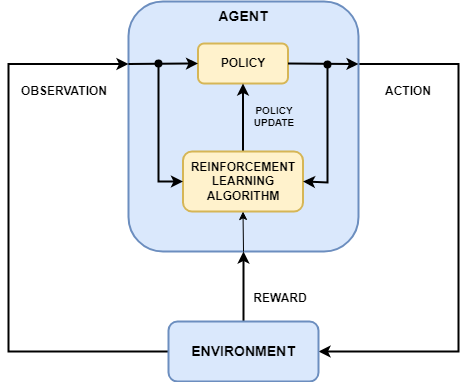
\includegraphics[width=0.75\textwidth]{photos/reinforcement_learning_diagram.png}
  \caption{چارچوب کلی یادگیری تقویتی~\cite{mathworksRLdiag2025}.}
  \label{fig:rl_framework}
\end{figure}

\begin{itemize}
    \item \textbf{عامل:} یادگیرنده یا تصمیم‌گیرنده. در معامله‌گری الگوریتمی، عامل همان راهبرد معاملاتی است که عمل‌های خرید، فروش یا نگه‌داشتن را انتخاب می‌کند.
    
    \item \textbf{محیط:} سامانه خارجی که عامل با آن تعامل دارد. در کاربردهای مالی، محیط معمولاً بازار است که شامل پویایی قیمت، دفتر سفارش و داده‌های احساسی می‌شود.
    
    \item \textbf{حالت ($s_t$):} بازنمایی وضعیت محیط در زمان $t$. در معامله‌گری، حالت‌ها می‌توانند شامل شاخص‌های فنی  وامتیازهای احساسی استخراج‌شده از اخبار و داده‌های تاریخی باشند.
    
    \item \textbf{عمل ($a_t$):} مجموعه تصمیم‌های در دسترس عامل در زمان $t$. در ساده‌ترین حالت، این مجموعه شامل $\{ \text{خرید، فروش، نگه‌داشتن} \}$ است، اما می‌تواند به بازتخصیص سبد سهام یا تعیین اندازه موقعیت به‌صورت پیوسته نیز گسترش یابد.
    
    \item \textbf{پاداش ($r_t$):} سیگنال بازخورد عددی که سود یا زیان فوری ناشی از اجرای عمل $a_t$ در حالت $s_t$ را نشان می‌دهد. در زمینه مالی، این معمولاً به‌صورت \textbf{سود و زیان}، بازدهی تعدیل‌شده بر اساس ریسک یا تابعی سفارشی تعریف می‌شود که اهداف مدیریت ریسک را نیز در نظر می‌گیرد.
    
    \item \textbf{سیاست ($\pi$):} راهبرد عامل برای نگاشت حالت‌ها به عمل‌ها. سیاست‌ها می‌توانند \textbf{قطعی} باشند ($a = \pi(s)$) یا \textbf{تصادفی} باشند ($a \sim \pi(\cdot|s)$).
    
    \item \textbf{تابع ارزش:} برآورد پاداش تجمعی مورد انتظار هنگام شروع از یک حالت یا جفت حالت ـ عمل مشخص. این تابع معیاری از مطلوبیت بلندمدت حالت‌ها، فراتر از پاداش‌های فوری ارائه می‌دهد.
    
    \item \textbf{مدل محیط:} یک مؤلفه اختیاری که انتقال حالت‌ها را بر اساس عمل‌ها پیش‌بینی می‌کند. رویکردهای \textbf{مدل‌نا‌مبنا}\LTRfootnote{Model-Free} مانند \lr{Proximal Policy Optimization, PPO} محیط را به‌طور صریح مدل‌سازی نمی‌کنند، در حالی که روش‌های \textbf{مدل‌مبنا}\LTRfootnote{Model-Based} چنین مدل‌های پیش‌بینی را در نظر می‌گیرند.
\end{itemize}

این اجزا شالوده الگوریتم‌های یادگیری تقویتی را تشکیل می‌دهند. در معامله‌گری مالی، طراحی دقیق فضای حالت، مجموعه عمل و تابع پاداش اهمیت حیاتی دارد؛ زیرا تعریف‌های ضعیف یا نادرست می‌توانند به پویایی‌های یادگیری ناپایدار یا راهبردهای معاملاتی زیان‌ده منجر شوند.

\subsection{اکتشاف\protect\LTRfootnote{\lr{Exploration}} در برابر بهره‌برداری\protect\LTRfootnote{\lr{Exploitation}}}

یکی از چالش‌های اصلی در \textbf{یادگیری تقویتی} موازنه میان \textbf{اکتشاف} و \textbf{بهره‌برداری} است.  

\begin{itemize}
    \item \textbf{اکتشاف:} فرآیند انتخاب عمل‌هایی با قطعیت کمتر برای کسب دانش جدید و احتمالاً کشف راهبردهایی که بازدهی بلندمدت بیشتری ایجاد می‌کنند. در معامله‌گری، اکتشاف می‌تواند شامل آزمون شاخص‌ها یا سیگنال‌های جدید بازار باشد، حتی اگر سودآوری فوری آن‌ها نامشخص باشد.
    
    \item \textbf{بهره‌برداری:} فرآیند استفاده از دانش موجود برای بیشینه‌سازی پاداش مورد انتظار از طریق انتخاب مداوم عمل‌هایی که بهترین عملکرد برآوردشده را دارند. در کاربردهای مالی، این به معنای انجام معاملاتی است که در گذشته بازدهی قوی نشان داده‌اند.
\end{itemize}

\begin{figure}[htbp]
  \centering
  
\includegraphics[width=0.75\textwidth]{photos/exp_vs_exp.jpg}
  \caption{نمایی از موازنه اکتشاف ـ بهره‌برداری~\cite{huggingfaceExp2RL2025}.}
  \label{fig:exp2_rl}
\end{figure}

تعادل میان اکتشاف و بهره‌برداری حیاتی است. بهره‌برداری بیش از حد می‌تواند به همگرایی زودهنگام بر سیاست‌های زیربهینه منجر شود و عملکرد بلندمدت را محدود کند. در مقابل، اکتشاف بیش از حد ممکن است به رفتار ناپایدار و افزایش مواجهه با ریسک بیانجامد ـ موضوعی که در بازارهای مالی اهمیت ویژه‌ای دارد.  

\subsection{وظایف رویدادمحور\protect\LTRfootnote{\lr{Episodic Tasks}} در برابر وظایف پیوسته\protect\LTRfootnote{\lr{Continuous Tasks}}}

مسائل \textbf{یادگیری تقویتی} را می‌توان به‌طور کلی به \textbf{وظایف رویدادمحور} \textbf{وظایف پیوسته} تقسیم کرد که بر اساس نحوه تعامل عامل با محیط تعریف می‌شوند.

\begin{itemize}
    \item \textbf{وظایف رویدادمحور:} تعامل به دوره‌های گسسته تقسیم می‌شود که هرکدام حالت آغازین و پایانی مشخص دارند. در پایان هر دوره، محیط بازنشانی می‌شود و فرآیند یادگیری دوباره آغاز می‌گردد. نمونه‌های کلاسیک شامل بازی‌های تخته‌ای مانند شطرنج و \lr{Go} هستند که هر مسابقه یک دوره محسوب می‌شود. در معامله‌گری مالی، یک افق سرمایه‌گذاری ثابت (مثلاً شبیه‌سازی ۳۰ روز معاملاتی) را می‌توان به‌عنوان یک وظیفه رویداد محور مدل کرد.
    
    \item \textbf{وظایف پیوسته:} تعامل به‌طور نامحدود ادامه دارد، بدون اینکه حالت پایانی طبیعی داشته باشد. عامل باید رفتار خود را در یک جریان بی‌پایان از حالت‌ها و پاداش‌ها بهینه کند. بازارهای مالی ذاتاً پیوسته‌اند، زیرا فرصت‌های معاملاتی و حرکت‌های قیمتی بدون نقطه پایان از پیش تعیین‌شده در جریان هستند.
\end{itemize}

این تمایز به‌طور مستقیم بر نحوه محاسبه توابع ارزش اثر می‌گذارد. در وظایف رویدادمحور معمولاً پاداش‌ها تا یک نقطه پایان مشخص جمع می‌شوند (بازدهی با افق محدود). اما در وظایف پیوسته از بازدهی تنزیل‌شده با افق نامحدود استفاده می‌شود تا مجموع پاداش‌ها همواره مقدار محدودی داشته باشد:
\[
G_t = \sum_{k=0}^{\infty} \gamma^k r_{t+k+1}, \quad 0 \leq \gamma < 1,
\]

که در آن $\gamma$ \textbf{ضریب تنزیل}\protect\LTRfootnote{\lr{Discount Factor}} است و موازنه میان پاداش‌های فوری و بلندمدت را کنترل می‌کند.

در معامله‌گری الگوریتمی، محیط‌ها غالباً به‌صورت پیوسته مدل می‌شوند تا ماهیت همیشگی بازار بازتاب یابد. با این حال، فرآیند آموزش معمولاً در قالب دوره‌ها (مانند دوره‌های سالانه یا فصلی) سازمان‌دهی می‌شود تا یادگیری پایدارتر گردد، ارزیابی تسهیل شود و مقایسه میان راهبردها امکان‌پذیر باشد.  

\subsection{یادگیری درون‌سیاستی\protect\LTRfootnote{\lr{On-Policy Learning}} در برابر برون‌سیاستی\protect\LTRfootnote{\lr{Off-Policy Learning}}}

الگوریتم‌های \textbf{یادگیری تقویتی} را می‌توان به \textbf{روش‌های درون‌سیاستی} و \textbf{روش‌های برون‌سیاستی} تقسیم کرد. این دسته‌بندی بر اساس نحوه بهبود سیاست عامل تعریف می‌شود.  

\begin{itemize}
    \item \textbf{یادگیری درون‌سیاستی:} عامل ارزش سیاستی را می‌آموزد که هم‌اکنون در حال اجراست. داده‌ها با پیروی از همین سیاست جمع‌آوری می‌شوند و بهبودها بر همان اساس صورت می‌گیرد. نمونه‌ها شامل \lr{SARSA} و روش‌های \textbf{گرادیان سیاست}\LTRfootnote{Policy Gradient Methods} مانند \lr{Proximal Policy Optimization, PPO} هستند. در معامله‌گری الگوریتمی، این به عاملی اشاره دارد که بر اساس معاملاتی که تحت راهبرد جاری خود انجام می‌دهد، تطبیق پیدا می‌کند.
    
    \item \textbf{یادگیری برون‌سیاستی:} عامل ارزش یک سیاست بهینه را می‌آموزد، حتی اگر از یک سیاست رفتاری متفاوت پیروی کند. این رویکرد امکان یادگیری از داده‌های تاریخی، نمایش‌ها یا رفتارهای اکتشافی را فراهم می‌آورد. نمونه‌های بارز شامل \lr{Q-learning} و \lr{Deep Q-Networks, DQN} هستند. در معامله‌گری، این روش به عامل اجازه می‌دهد از داده‌های تاریخی گسترده بازار بیاموزد، بدون آنکه معاملات را در زمان واقعی اجرا کند.
\end{itemize}

روش‌های درون‌سیاستی معمولاً پایدارتر و ایمن‌تر در حوزه‌های پرریسک مانند معامله‌گری هستند، در حالی که روش‌های برون‌سیاستی داده‌محورتر بوده و می‌توانند از تجربیات گذشته و شبیه‌سازی‌های برون‌خط استفاده کنند~\cite{sutton2018reinforcement}.  


\subsection{روش‌های مدل‌مبنا\protect\LTRfootnote{\lr{Model-Based Methods}} در برابر مدل‌نامبنا\protect\LTRfootnote{\lr{Model-Free Methods}}}

تمایز مهم دیگر در یادگیری تقویتی میان \textbf{روش‌های مدل‌نا‌مبنا} و \textbf{روش‌های مدل‌مبنا} است. این تمایز بر اساس صریح‌بودن یا نبودن مدل‌سازی محیط تعریف می‌شود. 
 
\begin{itemize}
    \item \textbf{روش‌های بدون‌مدل:} این الگوریتم‌ها تلاشی برای یادگیری ساختار انتقال محیط نمی‌کنند، بلکه مستقیماً توابع ارزش یا سیاست‌ها را از طریق تعامل تخمین می‌زنند. نمونه‌هایی از این دسته شامل \lr{Q-learning}، \lr{DQN} و \lr{PPO} هستند. در معامله‌گری، یک عامل بدون‌مدل مستقیماً از داده‌های بازار مانند سری‌های قیمتی، شاخص‌ها و سیگنال‌های احساسی یاد می‌گیرد، بدون آنکه مسیر آینده بازار را پیش‌بینی کند.
    
    \item \textbf{روش‌های مبتنی‌بر‌مدل:} این رویکردها بر یادگیری یا استفاده از یک مدل پیش‌بینی‌کننده رفتار محیط (مانند احتمال‌های گذار بین حالت‌ها و تابع پاداش) تکیه دارند. چنین مدل‌هایی امکان به‌کارگیری تکنیک‌های برنامه‌ریزی مانند \textbf{برنامه‌ریزی پویا}\LTRfootnote{Dynamic Programming} یا \textbf{جستجوی درختی مونت‌کارلو}\LTRfootnote{Monte Carlo Tree Search, MCTS} را فراهم می‌کنند. در حوزه مالی، این می‌تواند شامل ساخت مدل‌های پیش‌بینی تغییرات قیمت دارایی‌ها یا شبیه‌سازی رفتار دفتر سفارش برای هدایت تصمیم‌گیری باشد.
\end{itemize}

به طور کلی، روش‌های بدون‌مدل ساده‌تر بوده و با یادگیری عمیق بهتر مقیاس‌پذیر هستند، هرچند به داده و فرآیند اکتشاف بیشتری نیاز دارند. در مقابل، روش‌های مبتنی‌بر‌مدل از نظر استفاده از داده کاراترند، اما نسبت به خطاهای مدل حساسیت بیشتری دارند ـ موضوعی که در بازارهای مالی پرتلاطم و ناپایدار اهمیت ویژه‌ای پیدا می‌کند.


\section{الگوریتم‌های یادگیری تقویتی}

\subsection{\lr{Q-Learning} و شبکه‌های \lr{Q} عمیق\protect\footnotemark}
\footnotetext{\lr{Deep Q-Networks, DQN}}

\lr{Q-Learning} که نخستین‌بار توسط \lr{Watkins} در سال 1989 معرفی شد~\cite{watkins1989q}، یکی از الگوریتم‌های بنیادی در \textbf{یادگیری تقویتی} است. این روش \textbf{برون‌سیاستی} و \textbf{مدل‌نا‌مبنا} است و هدف آن یادگیری تابع ارزش عمل بهینه $Q^*(s, a)$ می‌باشد. این تابع بیانگر پاداش تجمعی تنزیل‌شده مورد انتظار از انتخاب عمل $a$ در حالت $s$ و سپس پیروی از سیاست بهینه است. قاعده به‌روزرسانی \lr{Q-learning} به‌صورت زیر تعریف می‌شود:

\[
Q(s_t, a_t) \leftarrow Q(s_t, a_t) + \alpha \Big[ r_{t+1} + \gamma \max_{a'} Q(s_{t+1}, a') - Q(s_t, a_t) \Big]
\]

که در آن $\alpha$ \textbf{نرخ یادگیری}\LTRfootnote{Learning Rate}، $\gamma$ \textbf{ضریب تنزیل}\LTRfootnote{Discount Factor} و $r_{t+1}$ پاداش دریافتی پس از اجرای عمل $a_t$ در حالت $s_t$ است.  

\bigskip

\textbf{شبکه‌های \lr{Q} عمیق}\LTRfootnote{Deep Q-Networks, DQN} بسط \lr{Q-learning} هستند که در آن تابع $Q$ با استفاده از یک شبکه عصبی عمیق تقریب زده می‌شود. این رویکرد امکان مقیاس‌پذیری به فضاهای ورودی با ابعاد بالا مانند تصاویر یا سری‌های زمانی مالی را فراهم می‌کند. پژوهش برجسته \lr{Mnih et al. (2015)}~\cite{mnih2015human} موفقیت \lr{DQN} را در یادگیری مستقیم از ورودی‌های خام پیکسلی در بازی‌های آتاری نشان داد. نوآوری‌های کلیدی \lr{DQN} شامل موارد زیر است:  

\begin{itemize}
\item \textbf{بازپخش تجربه}\LTRfootnote{Experience Replay}: انتقال‌ها $(s, a, r, s')$ در یک حافظه بازپخش ذخیره می‌شوند و آموزش شبکه با استفاده از \textbf{بسته‌های کوچک داده} که به‌طور تصادفی از این حافظه نمونه‌برداری می‌شوند انجام می‌شود. این فرآیند همبستگی میان به‌روزرسانی‌های متوالی را کاهش داده و پایداری آموزش را افزایش می‌دهد.

    \item \textbf{شبکه‌های هدف}: یک شبکه هدف جداگانه برای محاسبه مقادیر هدف در \lr{Q-learning} به‌کار گرفته می‌شود که به‌صورت دوره‌ای به‌روزرسانی می‌گردد. این رویکرد از نوسانات مخرب و واگرایی در طول آموزش جلوگیری می‌کند.
\end{itemize}

\bigskip

در کاربردهای معاملاتی، \lr{Q-learning} و \lr{DQN} می‌توانند برای یادگیری سیاست‌هایی مورد استفاده قرار گیرند که مشخص می‌کنند آیا عامل باید دارایی را بخرد، بفروشد یا نگه دارد؛ بر اساس حالتی که توسط شاخص‌های بازار، امتیازهای احساسی و داده‌های قیمتی تعریف می‌شود. با این حال، بازارهای مالی چالش‌های خاصی برای \lr{DQN}  ایجاد می‌کنند، زیرا حالت‌ها پیوسته، غیرایستا و پاداش‌ها تصادفی هستند؛ بنابراین تصمیم‌گیری حساس به ریسک ضرورت می‌یابد. با وجود این محدودیت‌ها، \lr{DQN}  همچنان به‌عنوان یک معیار مرجع ارزشمند در مقایسه با روش‌های پیشرفته‌تر مانند \textbf{گرادیان سیاست} و رویکردهای \textbf{بازیگر \lr{-} منتقد} به‌کار می‌رود.  


\subsection{روش‌های گرادیان سیاست\protect\footnotemark}
\footnotetext{\lr{Policy Gradient Methods}}

در حالی که روش‌های مبتنی بر ارزش مانند \lr{Q-learning} به تخمین \textbf{تابع ارزش عمل} می‌پردازند، \textbf{روش‌های گرادیان سیاست}\LTRfootnote{Policy Gradient Methods} مستقیماً سیاست $\pi_{\theta}(a|s)$ را که با پارامترهای $\theta$ (مانند وزن‌های یک شبکه عصبی) مشخص می‌شود، بهینه می‌کنند. هدف اصلی، بیشینه‌سازی بازدهی مورد انتظار است:

\[
J(\theta) = \mathbb{E}_{\pi_\theta}\bigg[ \sum_{t=0}^\infty \gamma^t r_t \bigg],
\]

که گرادیان‌ها بر اساس \textbf{قضیه گرادیان سیاست}\LTRfootnote{Policy Gradient Theorem} به‌دست می‌آیند~\cite{sutton1999policy}:

\[
\nabla_\theta J(\theta) = \mathbb{E}_{\pi_\theta}\big[ \nabla_\theta \log \pi_\theta(a_t|s_t) \, G_t \big],
\]

که در آن $G_t$ بازدهی پس از گام زمانی $t$ را نشان می‌دهد.  

\bigskip

\textbf{مزایای روش‌های گرادیان سیاست:}
\begin{itemize}
    \item قابلیت طبیعی در مدیریت فضاهای عمل \textbf{پیوسته} و با ابعاد بالا، در حالی که روش‌های مبتنی بر ارزش معمولاً به عمل‌های گسسته محدودند.
    \item پشتیبانی از سیاست‌های \textbf{تصادفی} که فرآیند اکتشاف را تسهیل می‌کنند.
    \item امکان ادغام مستقیم محدودیت‌ها، معیارهای ریسک یا هزینه‌های تراکنش در طراحی پاداش.
\end{itemize}

\textbf{چالش‌ها:}
\begin{itemize}
\item برآورد گرادیان در این روش‌ها معمولاً نوسان زیادی دارد (\textbf{واریانس بالا}\LTRfootnote{High Variance})، به همین دلیل لازم است از \textbf{روش‌های کاهش واریانس}\LTRfootnote{Variance Reduction Techniques} مانند استفاده از \textbf{مبناها}\LTRfootnote{Baselines} یا \textbf{توابع برتری}\LTRfootnote{Advantage Functions} کمک گرفته شود تا پایداری آموزش افزایش یابد.  

\item این الگوریتم‌ها در مقایسه با روش‌های \textbf{برون‌سیاستی} مانند \lr{DQN}، به داده‌های بیشتری برای یادگیری نیاز دارند و از نظر کارایی استفاده از نمونه‌ها ضعیف‌تر عمل می‌کنند.
\end{itemize}

\bigskip

در معامله‌گری مالی، روش‌های گرادیان سیاست به‌ویژه اهمیت دارند زیرا عمل‌ها (مانند وزن‌های سبد سهام یا اندازه موقعیت‌ها) ذاتاً پیوسته‌اند. برای نمونه، یک عامل یادگیری تقویتی می‌تواند به‌طور مستقیم کسری از سرمایه را که باید میان دارایی‌های مختلف تخصیص یابد، خروجی دهد. الگوریتم‌های اولیه‌ای مانند \lr{REINFORCE}~\cite{williams1992simple} بنیان این حوزه را شکل دادند، در حالی که بسط‌های مدرن مانند روش‌های بازیگر\lr{-}منتقد پایداری و کارایی بیشتری به همراه داشته‌اند.  

\subsection{روش‌های بازیگر \lr{-} منتقد\protect\footnotemark}
\footnotetext{\lr{Actor–Critic Methods}}

روش‌های \textbf{بازیگر \lr{-} منتقد} مزایای رویکردهای مبتنی بر ارزش و مبتنی بر سیاست را در \textbf{یادگیری تقویتی} ترکیب می‌کنند. این روش‌ها از دو مؤلفه اصلی تشکیل شده‌اند~\cite{konda2000actor}:  

\begin{itemize}
    \item \textbf{بازیگر (\lr{Actor}):} تابع سیاست $\pi_{\theta}(a|s)$ با پارامترهای $\theta$ که عمل‌ها را بر اساس حالت‌ها انتخاب می‌کند.
    \item \textbf{منتقد (\lr{Critic}):} تابع ارزش $V^{\pi}(s)$ یا تابع ارزش عمل $Q^{\pi}(s,a)$ با پارامترهای $\phi$ که کیفیت سیاست را از طریق برآورد بازدهی مورد انتظار ارزیابی می‌کند.
\end{itemize}

منتقد در این چارچوب نقشی مانند یک \textbf{مبنا}\LTRfootnote{Baseline} دارد و کمک می‌کند تا نوسان زیاد (واریانس) در برآورد گرادیان سیاست کاهش یابد. بازیگر وظیفه دارد پارامترهای سیاست را در جهتی که \textbf{قضیه گرادیان سیاست}\LTRfootnote{Policy Gradient Theorem} مشخص کرده به‌روزرسانی کند. در مقابل، منتقد با استفاده از \textbf{یادگیری تفاضل زمانی}\LTRfootnote{Temporal-Difference, TD Learning} مقدارهای ارزش را بهبود می‌دهد و بازخورد دقیق‌تری به بازیگر می‌دهد.  

به‌طور خلاصه، به‌روزرسانی رایج بازیگر به صورت زیر نوشته می‌شود:

\[
\nabla_\theta J(\theta) \approx \mathbb{E}_{\pi_\theta}\big[ \nabla_\theta \log \pi_\theta(a_t|s_t) \, A^{\pi}(s_t, a_t) \big],
\]

که در آن $A^{\pi}(s_t, a_t)$ \textbf{تابع برتری}\LTRfootnote{Advantage Function} است. این تابع نشان می‌دهد که یک عمل در وضعیت خاص، نسبت به میانگین انتظاری (مبنا) تا چه حد بهتر یا بدتر است. به این ترتیب، بازیگر به سمت اعمالی متمایل می‌شود که ارزش بیشتری نسبت به مبنا دارند.

\bigskip

\textbf{مزایای روش‌های بازیگر\lr{-}منتقد}
\begin{itemize}
    \item کارایی نمونه‌ای بیشتر نسبت به روش‌های صرفاً گرادیان سیاست مانند \lr{REINFORCE}، به دلیل کاهش واریانس توسط منتقد.
    \item مقیاس‌پذیری به فضاهای عمل پیوسته و با ابعاد بزرگ.
\item ایجاد بنیان برای الگوریتم‌های پیشرفته‌ای مانند \lr{A2C}، \lr{A3C} و \lr{PPO}.
\end{itemize}

\bigskip

روش‌های بازیگر\lr{-}منتقد به‌ویژه در معامله‌گری مالی کارآمد هستند؛ زیرا منتقد با ارائه برآوردهای دقیق‌تر از بازدهی، یادگیری را در بازارهای پرنوسان و غیرایستا پایدارتر می‌سازد. برای نمونه، بازیگر می‌تواند معاملاتی مانند تنظیم اندازه موقعیت‌ها را پیشنهاد دهد، در حالی که منتقد سودآوری بلندمدت آن‌ها را ارزیابی می‌کند. بسط‌هایی مانند \lr{A3C} نیز امکان آموزش موازی در چندین بازار شبیه‌سازی‌شده را فراهم کرده و کارایی و پایداری فرآیند یادگیری را افزایش می‌دهند.  


\subsection{\lr{Proximal Policy Optimization (PPO)}}

الگوریتم \lr{PPO}~\cite{schulman2017proximal} یکی از پرکاربردترین روش‌های \textbf{گرادیان سیاست} است که به دلیل پایداری، سادگی و عملکرد تجربی قوی شناخته می‌شود. این الگوریتم در خانواده روش‌های \textbf{بازیگر \lr{-} منتقد} قرار می‌گیرد، اما سازوکاری برای محدود کردن به‌روزرسانی‌های بیش از حد سیاست معرفی می‌کند؛ زیرا چنین به‌روزرسانی‌هایی می‌توانند آموزش را ناپایدار سازند.

ایده اصلی، بهینه‌سازی یک \textbf{تابع هدف جانشین} با استفاده از \textbf{نسبت احتمالات برش‌خورده}\LTRfootnote{Clipped Probability Ratio} است:  

\[
L^{CLIP}(\theta) = \mathbb{E}_t \Big[ 
    \min\big( r_t(\theta) A_t,\,
    clip(r_t(\theta), 1-\epsilon, 1+\epsilon) A_t \big)
\Big],
\]

که در آن:
\begin{itemize}
    \item $r_t(\theta) = \tfrac{\pi_\theta(a_t|s_t)}{\pi_{\theta_old}(a_t|s_t)}$ نسبت احتمالات است،
    \item $A_t$ \textbf{تابع برتری} برآوردشده است،
    \item $\epsilon$ پارامتر برش است (معمولاً در بازه $0.1$ تا $0.2$).
\end{itemize}

برش‌زدن مانع می‌شود که سیاست جدید در یک به‌روزرسانی بیش از حد از سیاست قدیم منحرف شود و به این ترتیب یادگیری پایدارتر می‌گردد. افزون بر این، \lr{PPO} اغلب از \textbf{منظم‌سازی آنتروپی}\LTRfootnote{Entropy Regularization} برای تقویت اکتشاف بهره می‌گیرد.  

\bigskip
\textbf{تابع زیان کلی:}  
در عمل، \lr{PPO} چندین مؤلفه را در یک تابع زیان ترکیب می‌کند:  

\[
L^{PPO}(\theta) = \mathbb{E}_t \Big[ 
    L^{CLIP}(\theta) 
    - c_1 \big( V_\theta(s_t) - V_t^{target} \big)^2 
    + c_2 H\big( \pi_\theta(\cdot|s_t) \big)
\Big],
\]

که در آن:  
\begin{itemize}
    \item $L^{CLIP}(\theta)$ زیان سیاست برش‌خورده است،
    \item $\big( V_\theta(s_t) - V_t^{target} \big)^2$ خطای مربعی میان برآورد منتقد و بازدهی هدف است،
    \item $H(\pi_\theta(\cdot|s_t))$ آنتروپی سیاست است که اکتشاف را تشویق می‌کند،
    \item $c_1$ و $c_2$ ضرایب کنترل‌کننده اهمیت مؤلفه‌های ارزش و آنتروپی هستند.
\end{itemize}

\textbf{مزایای \lr{PPO}:}
\begin{itemize}
    \item موازنه مؤثر میان اکتشاف و بهره‌برداری،  
    \item ساده‌تر و مقاوم‌تر نسبت به روش‌های پیشین مبتنی بر ناحیه اعتماد مانند \lr{TRPO}،  
    \item مقیاس‌پذیری مناسب در ترکیب با شبکه‌های عصبی عمیق و مسائل با ابعاد بالا.  
\end{itemize}

\lr{PPO} به‌ویژه برای محیط‌های معاملاتی مالی مناسب است؛ جایی که پایداری و مقاوم‌بودن اهمیت بالایی دارند زیرا داده‌ها پرنویز و غیرایستا هستند. با کنترل دقیق به‌روزرسانی‌های سیاست و ترکیب مؤلفه‌های سیاست، ارزش و آنتروپی، \lr{PPO} امکان سازگاری تدریجی راهبردهای معاملاتی را فراهم می‌کند و میان بیشینه‌سازی سود، مدیریت ریسک و اکتشاف فرصت‌های جدید تعادل برقرار می‌سازد.  
  

\subsection{\lr{PPO} بازگشتی\protect}
\LTRfootnote{\lr{Recurrent PPO}}

بسیاری از محیط‌های دنیای واقعی ــ از جمله بازارهای مالی ــ دارای \textbf{قابلیت مشاهده ناقص}\LTRfootnote{Partial Observability} هستند؛ به این معنا که عامل مستقیماً حالت زیربنایی را مشاهده نمی‌کند، بلکه تنها سیگنال‌های نویزی یا ناقصی مانند قیمت‌ها، شاخص‌های احساسی یا ویژگی‌های فنی دریافت می‌کند. برای رفع این چالش، الگوریتم \lr{PPO} را می‌توان با \textbf{شبکه‌های عصبی بازگشتی} بسط داد که منجر به \textbf{\lr{PPO} بازگشتی} می‌شود~\cite{heess2015memory_arxiv}.  

در \lr{RPPO} شبکه‌های سیاست و ارزش با مؤلفه‌های حافظه‌ای مانند \lr{LSTM} یا \lr{GRU} تقویت می‌شوند. این ساختار به عامل امکان می‌دهد \textbf{وابستگی‌های زمانی}\LTRfootnote{Temporal Dependencies} را ثبت کرده و یک \textbf{حالت پنهان}\LTRfootnote{Hidden State} را در طول گام‌های زمانی حفظ کند. حالت پنهان اطلاعات گذشته مرتبط را خلاصه می‌کند و در نتیجه تصمیم‌گیری مؤثرتری را در شرایط مشاهده ناقص ممکن می‌سازد.  

\textbf{مزایای \lr{PPO} بازگشتی:}
\begin{itemize}
    \item توانایی مدیریت مشاهده ناقص از طریق حفظ حافظه شرایط گذشته بازار.  
    \item بهبود عملکرد در وظایف دنباله‌ای با وابستگی‌های بلندمدت.  
    \item ارائه چارچوبی واقع‌بینانه‌تر برای معامله‌گری مالی، جایی که تصمیم‌ها هم به بستر تاریخی و هم به سیگنال‌های جاری وابسته‌اند.  
\end{itemize}

الگوریتم \lr{RPPO} توانایی عامل معاملاتی مبتنی بر یادگیری تقویتی را در تشخیص الگوهای زمانی موجود در داده‌های مالی افزایش می‌دهد. برای نمونه، گاهی قیمت‌ها تمایل دارند مدتی در همان جهت قبلی حرکت کنند (اثر تداوم روند)، یا دوره‌های پرنوسان و کم‌نوسان بازار معمولاً پشت سر هم رخ می‌دهند. با ترکیب شاخص‌های فنی و ویژگی‌های احساسی در یک ساختار بازگشتی، \lr{RPPO} می‌تواند این الگوهای زمانی را بهتر از نسخه استاندارد \lr{PPO} (بدون حافظه بازگشتی) ثبت کرده و راهبردهای معاملاتی سازگارتر ارائه دهد.


\section{مبانی مدل‌های زبانی بزرگ}

\subsection{معماری \lr{Transformer}}

\lr{Transformer}~\cite{vaswani2017attention} یک معماری یادگیری عمیق است که بنیان مدل‌های زبانی بزرگ مدرن را تشکیل می‌دهد. برخلاف \textbf{شبکه‌های عصبی بازگشتی} یا \textbf{مدل‌های کانولوشنی}\LTRfootnote{\lr{Convolutional Models}}، \lr{Transformer} کاملاً بر \textbf{سازوکار خودتوجهی}\LTRfootnote{\lr{Self-Attention Mechanism}} متکی است تا وابستگی میان واحدهای زبانی در متن را ثبت کند. این ویژگی امکان موازی‌سازی کارآمد و مقیاس‌پذیری تا مجموعه‌داده‌های بسیار بزرگ را فراهم می‌سازد.

\bigskip
\textbf{اجزای کلیدی معماری \lr{Transformer}:}

\begin{itemize}
    \item \textbf{تعبیه ورودی}\LTRfootnote{\lr{Input Embeddings}}: هر واحد زبانی در دنباله به یک بردار متراکم نگاشت می‌شود. از آنجا که \lr{Transformer}ها فاقد بازگشت یا کانولوشن هستند، \textbf{کدگذاری‌های مکانی}\LTRfootnote{\lr{Positional Encodings}} به این بردارها افزوده می‌شوند تا ترتیب واحد‌های زبانی حفظ شود.
    
\item \textbf{سازوکار خودتوجهی}: عملیات اصلی روابط میان همه جفت واحدهای زبانی در یک دنباله را محاسبه می‌کند. برای هر واحد زبانی، بردارهای پرسش ($Q$)، کلید ($K$) و مقدار ($V$) از نگاشت خطی تعبیه‌های ورودی به دست می‌آیند. توجه به صورت زیر محاسبه می‌شود:
\[
Attention(Q,K,V) = softmax\left(\frac{QK^\top}{\sqrt{d_k}}\right)V,
\]
که در آن $d_k$ بُعد بردارهای کلید است. این سازوکار به هر واحد زبانی اجازه می‌دهد بر اساس ارتباط معنایی به سایر واحدهای زبانی توجه کند.

\item \textbf{توجه چندسری}\LTRfootnote{\lr{Multi-Head Attention}}: به‌جای یک عملیات توجه منفرد، چندین توجه به‌طور موازی محاسبه می‌شوند که امکان ثبت انواع مختلفی از روابط را فراهم می‌کند. خروجی‌ها سپس به هم متصل شده و به فضای تعبیه بازافکنی می‌شوند.

\item \textbf{شبکه‌های پیشخور}\LTRfootnote{\lr{Feed-Forward Networks}}: بازنمایی هر موقعیت از یک شبکه عصبی تمام‌متصل با فعال‌ساز غیرخطی عبور می‌کند.

\item \textbf{اتصالات باقیمانده و نرمال‌سازی لایه}\LTRfootnote{\lr{Residual Connections \& Layer Normalization}}: برای پایدارسازی آموزش و بهبود جریان گرادیان، اتصالات باقیمانده پیرامون لایه‌های توجه و پیشخور اعمال می‌شوند و سپس نرمال‌سازی لایه انجام می‌شود.

\item \textbf{ساختار رمزگذار ـ رمزگشا}\LTRfootnote{\lr{Encoder–Decoder Structure}}: \lr{Transformer} اصلی شامل یک رمزگذار (مفید برای بازنمایی ورودی‌ها مانند ترجمه) و یک رمزگشا (مسئول تولید دنباله) است. مدل‌های زبانی بزرگی مانند \lr{GPT} از گونه \textbf{فقط رمزگشا}\LTRfootnote{\lr{Decoder-Only}} با سازوکار \lr{Masked Self-Attention} استفاده می‌کنند تا اطمینان یابند پیش‌بینی در گام $t$ تنها به واحدهای زبانی مشاهده‌شده تا آن لحظه وابسته باشد.

\end{itemize}


\subsection{جاسازی واژه‌ها\protect\LTRfootnote{\lr{Word Embeddings}} و جاسازی‌های متنی\protect\LTRfootnote{\lr{Text Embeddings}}}

مدل‌های \textbf{پردازش زبان طبیعی} برای عملکرد مناسب نیازمند بازنمایی عددی از واژه‌ها هستند تا معنای واژگانی در آن‌ها منعکس شود. این هدف با استفاده از \textbf{جاسازی‌ها} محقق می‌شود؛ یعنی نگاشت واحدهای گسسته به فضاهای برداری پیوسته که در آن‌ها روابط معنایی قابل اندازه‌گیری هستند.  

\bigskip
\textbf{جاسازی‌های ایستا}\LTRfootnote{\lr{Static Embeddings}}:  
روش‌های اولیه مانند \lr{Word2Vec}~\cite{mikolov2013efficient} و \lr{GloVe}~\cite{pennington2014glove} به هر واژه یک بردار ثابت اختصاص می‌دهند، مستقل از بافت آن. این جاسازی‌ها شباهت معنایی را از طریق حساب برداری ثبت می‌کنند. با این حال، جاسازی‌های ایستا قادر به ثبت \textbf{چندمعنایی}\LTRfootnote{\lr{Polysemy}} نیستند؛ یعنی واژه‌هایی با معانی متعدد صرف‌نظر از بافت تنها با یک بردار نمایش داده می‌شوند.  

\bigskip
\textbf{جاسازی‌های متنی}\LTRfootnote{\lr{Contextual Embeddings}}:  
مدل‌های مدرن مبتنی بر \lr{Transformer} مانند \lr{BERT}~\cite{devlin2019bert} و \lr{GPT}~\cite{radford2019language} جاسازی‌هایی تولید می‌کنند که \textbf{بافت‌محور} هستند. بازنمایی یک واژه بر اساس توکن‌های پیرامونی تغییر می‌کند و مدل را قادر می‌سازد میان معانی مختلف یک واژه تمایز قائل شود. این نوع جاسازی‌ها از سازوکار \textbf{خودتوجهی}\LTRfootnote{\lr{Self-Attention Mechanism}} برای ادغام اطلاعات معنایی در سراسر دنباله ورودی استفاده می‌کنند.  


\subsection{راهکارهای سازگار‌سازی مدل‌های زبانی بزرگ}

\textbf{مدل‌های زبانی بزرگ} پس از پیش‌آموزش عمومی، برای کارهای خاص نیاز به سازگار‌سازی دارند. مهم‌ترین رویکردها عبارت‌اند از:  

\begin{itemize}
    \item \textbf{ریزتنظیم}\LTRfootnote{\lr{Fine-tuning}}: ادامه آموزش روی داده‌های حوزه‌ای (مثلاً متون مالی) برای افزایش دقت در همان زمینه.  
    \item \textbf{تنظیم مبتنی بر دستور}\LTRfootnote{\lr{Instruction Tuning}}: آموزش مدل با داده‌های شامل «دستور + پاسخ» تا رفتار آن به نیت کاربر نزدیک‌تر شود.  
    \item \textbf{مهندسی دستور}\LTRfootnote{\lr{Prompt Engineering}}: طراحی ورودی‌های هوشمندانه توسط کاربر برای هدایت بهتر مدل، بدون نیاز به تغییر پارامترهای آن.  
\end{itemize}


\subsection{تحلیل احساسات در زمینه مالی\protect\footnotemark}

\textbf{تحلیل احساسات} فرآیند استخراج اطلاعات ذهنی ــ مانند نظرات، نگرش‌ها یا هیجانات ــ از داده‌های متنی است. در حوزه مالی، تحلیل احساسات به‌دنبال کمی‌سازی لحن عاطفی مقالات خبری، گزارش‌های تحلیلی یا بحث‌های شبکه‌های اجتماعی است؛ زیرا این منابع اغلب بر رفتار سرمایه‌گذاران و پویایی بازار اثرگذارند.  

\bigskip
\textbf{چرا احساسات اهمیت دارند:}  
بازارهای مالی صرفاً بر مبنای عوامل بنیادین هدایت نمی‌شوند، بلکه روان‌شناسی سرمایه‌گذاران و احساسات جمعی نیز نقشی تعیین‌کننده دارند. اخبار یا دیدگاه‌های مثبت می‌توانند حرکت‌های صعودی\LTRfootnote{\lr{Bullish}} را تقویت کنند، در حالی که احساسات منفی ممکن است به حرکت‌های نزولی\LTRfootnote{\lr{Bearish}} و فروش گسترده منجر شود. با تبدیل متن‌های غیرساختاریافته به امتیازهای ساختاریافته احساسات، عامل‌های معاملاتی قادر خواهند بود سیگنال‌های روان‌شناختی را در فرآیند تصمیم‌گیری سیستماتیک وارد کنند.

\bigskip

\textbf{روش‌های تحلیل احساسات:}
\begin{itemize}
    \item \textbf{روش‌های واژگانی}\LTRfootnote{\lr{Lexicon-based}}: بر پایه واژه‌نامه‌های از پیش تعریف‌شده برای کلمات مثبت و منفی. برای نمونه، واژه‌نامه \lr{Loughran–McDonald}~\cite{loughran2011liability} به‌طور گسترده در حوزه مالی استفاده می‌شود زیرا واژگان تخصصی این حوزه را پوشش می‌دهد.
    
    \item \textbf{روش‌های یادگیری ماشین سنتی}\LTRfootnote{\lr{Traditional Machine Learning}}: استفاده از ویژگی‌های مهندسی‌شده مانند \textbf{کیسه واژگان}\LTRfootnote{\lr{Bag-of-Words}} یا بازنمایی‌های \lr{TF–IDF} و ترکیب آن‌ها با دسته‌بندهایی مانند \lr{Logistic Regression} و \lr{Support Vector Machines (SVMs)}.
    
    \item \textbf{روش‌های یادگیری عمیق}\LTRfootnote{\lr{Deep Learning}}: مدل‌های مبتنی بر \lr{Transformer} مانند \lr{BERT} و \lr{FinBERT}~\cite{araci2019finbert} بازنمایی‌های بافت‌محور از متن تولید می‌کنند و نسبت به روش‌های پیشین عملکرد بهتری دارند. در ادامه، مدل‌های زبانی بزرگ\LTRfootnote{\lr{Large Language Models, LLMs}} مانند \lr{InstructGPT} و \lr{ChatGPT} معرفی شدند که بدون نیاز به ریزتنظیم گسترده می‌توانند تحلیل احساسات را در حالت \lr{Zero-shot} یا \lr{Few-shot} انجام دهند و به‌خوبی به متون مالی تطبیق یابند.
\end{itemize}

\bigskip

\textbf{ادغام سیگنال‌های احساسی در عامل‌های یادگیری تقویتی:}  
سیگنال‌های احساسی می‌توانند بخشی از بازنمایی حالت عامل‌های معاملاتی مبتنی بر \textbf{یادگیری تقویتی} باشند:  
\begin{itemize}
    \item احساسات مثبت احتمال اتخاذ موقعیت‌های خرید \LTRfootnote{Long} را افزایش می‌دهد.  
    \item احساسات منفی عامل را به سمت موقعیت‌های فروش \LTRfootnote{Short} یا کاهش ریسک هدایت می‌کند.  
    \item احساسات خنثی یا نامطمئن می‌تواند راهبردهای محافظه‌کارانه یا پوششی \LTRfootnote{Hedging} را تقویت کند.  
\end{itemize}

\bigskip
\textbf{چالش‌ها:}
\begin{itemize}
    \item زبان مالی دارای واژگان حوزه‌ای خاص است که ممکن است مدل‌های عمومی را گمراه کند.  
    \item طعنه، ابهام و ظرافت‌های زبانی هنوز به‌سختی توسط مدل‌ها شناسایی می‌شوند.  
    \item منابع خبری می‌توانند پرنویز، جانبدارانه یا دارای تأخیر باشند که قابلیت اطمینان سیگنال‌ها را کاهش می‌دهد.  
\end{itemize}

با وجود این چالش‌ها، تحلیل احساسات همچنان ابزاری قدرتمند برای تقویت راهبردهای معامله‌گری الگوریتمی باقی می‌ماند؛ به‌ویژه زمانی که در چارچوب‌های یادگیری تقویتی همراه با شاخص‌های فنی و داده‌های بازار به‌کار گرفته شود.  


\section{داده‌های بازار و شاخص‌های مالی}

\subsection{مبانی داده‌های \lr{OHLCV}\protect\footnotemark}
\footnotetext{\lr{Open, High, Low, Close, Volume}}

\textbf{داده‌های \lr{OHLCV}} نمایش استاندارد بازار مالی هستند که شامل قیمت باز، بیشینه، کمینه، بسته و حجم معاملات می‌شوند. این قالب، اساس تحلیل تکنیکال را تشکیل داده و به‌طور گسترده در معامله‌گری به‌کار گرفته می‌شود.  

\begin{itemize}
    \item \textbf{\lr{Open (O)}:} نخستین قیمت معامله‌شده یک دارایی در ابتدای بازه زمانی مشخص (مانند یک دقیقه، یک ساعت یا یک روز).  
    \item \textbf{\lr{High (H)}:} بیشترین قیمتی که در طول بازه زمانی ثبت شده است.  
    \item \textbf{\lr{Low (L)}:} کمترین قیمتی که در طول بازه زمانی ثبت شده است.  
    \item \textbf{\lr{Close (C)}:} آخرین قیمت معامله‌شده دارایی در پایان بازه زمانی.  
    \item \textbf{\lr{Volume (V)}:} مجموع حجم معامله‌شده دارایی در طول بازه زمانی، که بیانگر میزان فعالیت و نقدشوندگی بازار است.  
\end{itemize}

\bigskip
\textbf{نمایش داده‌ها:}  
داده‌های \lr{OHLCV} معمولاً با استفاده از \textbf{نمودار شمعی}\LTRfootnote{\lr{Candlestick Chart}} نمایش داده می‌شوند. در این نمودار، هر شمع قیمت‌های باز، بسته، بیشینه و کمینه را در یک بازه زمانی خلاصه می‌کند. ضخامت و رنگ بدنه شمع نشان‌دهنده صعودی بودن یا نزولی بودن قیمت در آن بازه است.  

\bigskip
\textbf{کاربردها:}
\begin{itemize}
    \item داده‌های \lr{OHLCV} ورودی خام برای شاخص‌های فنی متداول مانند محسوب می‌شوند.  
    \item این داده‌ها هم \textbf{پویایی‌های قیمت} (از طریق \lr{O}, \lr{H}, \lr{L}, \lr{C}) و هم \textbf{میزان مشارکت بازار} (از طریق \lr{V}) را منتقل می‌کنند.  
\item بسته به نوع راهبرد معاملاتی، داده‌ها می‌توانند در بازه‌های زمانی مختلف استفاده شوند؛ 
برای مثال داده‌های لحظه‌ای (تیک)، داده‌های درون‌روزی (ساعتی یا دقیقه‌ای)، داده‌های روزانه یا حتی هفتگی.
    \item در چارچوب‌های یادگیری تقویتی، مقادیر \lr{OHLCV} اغلب بخشی از فضای حالت هستند تا عامل بتواند از زمینه تاریخی ساختاریافته برای تصمیم‌گیری بهره ببرد.  
\end{itemize}

\bigskip
\textbf{محدودیت‌ها:}  
اگرچه داده‌های \lr{OHLCV} (قیمت باز، بسته، بالاترین، پایین‌ترین و حجم معاملات) اطلاعات کلی حرکت قیمت و حجم را نشان می‌دهند، اما جزئیات ریز بازار را پوشش نمی‌دهند. برای نمونه:  
- \textbf{عمق دفتر سفارش}\LTRfootnote{\lr{Order Book Depth}}: نشان می‌دهد چه تعداد سفارش خرید و فروش در سطوح مختلف قیمتی وجود دارد.  
- \textbf{شکاف خرید ـ فروش}\LTRfootnote{\lr{Bid–Ask Spread}}: اختلاف بین بالاترین قیمت پیشنهادی خریداران و پایین‌ترین قیمت پیشنهادی فروشندگان.  

این اطلاعات می‌توانند نقدشوندگی و فشار عرضه و تقاضا را بهتر نشان دهند. به همین دلیل، داده‌های \lr{OHLCV} معمولاً همراه با منابع تکمیلی ــ مانند شاخص‌های احساسی یا داده‌های بنیادین ــ به‌کار می‌روند تا قدرت پیش‌بینی و پایداری راهبردهای معامله‌گری الگوریتمی افزایش یابد.


\subsection{شاخص‌های فنی\protect\LTRfootnote{\lr{Technical Indicators}} پرکاربرد}

\textbf{شاخص‌های فنی} مقیاس‌های کمی مشتق‌شده از داده‌های \lr{OHLCV} هستند که معامله‌گران برای شناسایی \textbf{روندها}\LTRfootnote{\lr{Trends}}، \textbf{تکانه}\LTRfootnote{\lr{Momentum}}، \textbf{نوسان‌پذیری}\LTRfootnote{\lr{Volatility}} و نقاط احتمالی بازگشت به‌کار می‌گیرند. این شاخص‌ها هم در معامله‌گری اختیاری و هم در معامله‌گری الگوریتمی پرکاربردند و اغلب بخشی جدایی‌ناپذیر از فضای حالت برای عامل‌های یادگیری تقویتی محسوب می‌شوند.  

\bigskip
\textbf{شاخص‌های پیرو روند}\LTRfootnote{\lr{Trend-following}}:
\begin{itemize}
    \item \textbf{میانگین‌های متحرک}\LTRfootnote{\lr{Moving Averages, MA}}: میانگین قیمت‌های بسته‌شدن در یک پنجره زمانی ثابت. \textbf{میانگین متحرک ساده}\LTRfootnote{\lr{Simple Moving Average, SMA}} میانگینی بدون وزن است، در حالی که \textbf{میانگین متحرک نمایی}\LTRfootnote{\lr{Exponential Moving Average, EMA}} وزن بیشتری به قیمت‌های اخیر می‌دهد. تلاقی میانگین‌های کوتاه‌مدت و بلندمدت اغلب برای شناسایی تغییر روند استفاده می‌شود.  
\item \textbf{واگرایی ـ همگرایی میانگین متحرک}\LTRfootnote{\lr{Moving Average Convergence Divergence, MACD}}: 
این شاخص تفاوت بین دو میانگین متحرک نمایی (مثلاً ۱۲ و ۲۶ دوره‌ای) را نشان می‌دهد. 
وقتی این تفاوت محاسبه شد، یک میانگین متحرک کوتاه‌تر (مثلاً ۹ دوره‌ای) روی آن اعمال می‌شود که به آن «خط سیگنال» می‌گویند. 
تقاطع خط \lr{MACD} و خط سیگنال معمولاً به‌عنوان نشانه‌ای برای خرید یا فروش تفسیر می‌شود.

\end{itemize}

\bigskip
\textbf{شاخص‌های تکانه}\LTRfootnote{\lr{Momentum}}:
\begin{itemize}
    \item \textbf{شاخص قدرت نسبی}\LTRfootnote{\lr{Relative Strength Index, RSI}}: یک نوسان‌نما در بازه ۰ تا ۱۰۰ است که بزرگی نسبی سودها در برابر زیان‌های اخیر را اندازه‌گیری می‌کند. مقادیر بالاتر از ۷۰ معمولاً شرایط اشباع خرید و مقادیر پایین‌تر از ۳۰ شرایط اشباع فروش را نشان می‌دهند.  
\item \textbf{نوسان‌نمای تصادفی}\LTRfootnote{\lr{Stochastic Oscillator}}: 
این شاخص نشان می‌دهد قیمت بسته‌شدن یک دارایی در مقایسه با بالاترین و پایین‌ترین قیمت‌های اخیر در چه سطحی قرار دارد. 
اگر قیمت نزدیک سقف‌های اخیر باشد، نشانه‌ای از فشار خرید (اشباع خرید) است و اگر نزدیک کف‌های اخیر باشد، نشانه‌ای از فشار فروش (اشباع فروش) در نظر گرفته می‌شود.
\end{itemize}

\bigskip
\textbf{شاخص‌های نوسان‌پذیری}\LTRfootnote{\lr{Volatility}}:
\begin{itemize}
\item \lr{Bollinger Bands}: با قرار دادن باندهای بالا و پایین در چند انحراف معیار از یک میانگین متحرک ساخته می‌شوند. این باندها در دوره‌های پرنوسان گسترش یافته و در دوره‌های کم‌نوسان منقبض می‌شوند.  

\item \lr{Average True Range (ATR)}: نوسان‌پذیری را با میانگین‌گیری از دامنه واقعی (بیشترین اختلاف‌های \lr{High–Low}، \lr{High–Close} و \lr{Low–Close}) در یک دوره اندازه‌گیری می‌کند.
\end{itemize}

\bigskip
\textbf{شاخص‌های مبتنی بر حجم}\LTRfootnote{\lr{Volume-based}}:
\begin{itemize}
    \item \textbf{حجم تعادلی}\LTRfootnote{\lr{On-Balance Volume, OBV}}: یک معیار تجمعی است که در روزهای صعودی حجم معاملات را اضافه و در روزهای نزولی کم می‌کند تا فشار خرید و فروش را بازتاب دهد.  
    \item \textbf{میانگین موزون حجمی قیمت}\LTRfootnote{\lr{Volume-Weighted Average Price, VWAP}}: میانگین قیمت معامله‌شده یک دارایی است که بر اساس حجم وزن‌دهی می‌شود و اغلب به‌عنوان معیار کیفیت اجرا توسط معامله‌گران نهادی استفاده می‌گردد.  
\end{itemize}

\bigskip

برای عامل‌های یادگیری تقویتی، شاخص‌های فنی بازنمایی‌های سطح بالاتری از داده‌های \lr{OHLCV} فراهم می‌کنند و به عامل کمک می‌کنند الگوهایی مانند روندها، بازگشت‌ها یا رژیم‌های نوسان‌پذیری را که ممکن است در دنباله‌های خام قیمتی پنهان باشند شناسایی کند. ادغام این شاخص‌ها در فضای حالت می‌تواند کارایی یادگیری را از طریق تزریق دانش حوزه‌ای به مشاهدات عامل بهبود دهد.  

\bigskip
\textbf{محدودیت‌ها:}  
اگرچه شاخص‌های فنی می‌توانند بازنمایی حالت را غنی‌تر کنند، اما اتکای بیش از حد به آن‌ها می‌تواند منجر به فضاهای ویژگی با ابعاد بالا، نویز بیشتر و خطر \textbf{بیش‌برازش}\LTRfootnote{\lr{Overfitting}} شود. در عمل، انتخاب ویژگی محتاطانه، کاهش ابعاد یا استفاده از روش‌های یادگیری بازنمایی برای تضمین پایداری و مقاومت راهبردهای معاملاتی ضروری است.  


\subsection{چالش‌های موجود در بازارهای مالی}

به‌کارگیری \textbf{یادگیری تقویتی} در بازارهای مالی ذاتاً دشوار است؛ زیرا این محیط پیچیده، پویا و پر از نویز است. برخلاف وظایف معیار کنترل‌شده، بازارها موانع متعددی ایجاد می‌کنند که طراحی عامل‌های معاملاتی مقاوم را با چالش روبه‌رو می‌سازد.  

\bigskip
\textbf{ناایستایی}\LTRfootnote{\lr{Non-stationarity}}:  
ویژگی‌های آماری سری‌های زمانی مالی به‌مرور تغییر می‌کنند؛ به دلیل تغییر رژیم‌های بازار، چرخه‌های اقتصادی، تحولات مقرراتی و شوک‌های پیش‌بینی‌نشده. راهبردی که در یک رژیم (مانند بازار صعودی) موفق عمل می‌کند، ممکن است در شرایط متفاوت (مانند رکود یا بحران‌ها) ناکام بماند.  

\bigskip
\textbf{نسبت بالای نویز به سیگنال}\LTRfootnote{\lr{High Noise-to-Signal Ratio}}:  
قیمت دارایی‌ها تحت تأثیر عوامل متنوع و غیرقابل‌پیش‌بینی ــ از جمله اعلامیه‌های کلان اقتصادی، رویدادهای ژئوپولیتیکی و روان‌شناسی سرمایه‌گذاران ــ قرار دارند. تشخیص الگوهای معنادار از نوسانات تصادفی کاری بسیار دشوار است.  

\bigskip
\textbf{مشاهده ناقص}\LTRfootnote{\lr{Partial Observability}}:  
معامله‌گران به‌ندرت به وضعیت کامل بازار دسترسی دارند. متغیرهای پنهان مانند جریان سفارش‌های نهادی، اطلاعات خصوصی و محرک‌های نهفته بازار تأثیر چشمگیری بر پویایی‌ها دارند، اما برای عامل قابل مشاهده نیستند.  

\bigskip
\textbf{پاداش‌های پراکنده و با تأخیر}\LTRfootnote{\lr{Sparse and Delayed Rewards}}:  
فرصت‌های سودآور نسبت به تعداد کنش‌های معاملاتی ممکن، به‌ندرت رخ می‌دهند. بنابراین سیگنال‌های پاداش هم پراکنده و هم با تأخیر هستند و مسئله تخصیص اعتبار در آموزش یادگیری تقویتی را پیچیده می‌سازند.  

\bigskip
\textbf{هزینه‌های تراکنش}\LTRfootnote{\lr{Transaction Costs}} و \textbf{لغزش قیمتی}\LTRfootnote{\lr{Slippage}}:
اجرای واقعی معاملات مستلزم هزینه‌هایی مانند کمیسیون، \textbf{شکاف خرید ـ فروش} و تأثیر بازار است. راهبردهایی که در شبیه‌سازی سودآور به نظر می‌رسند، ممکن است پس از در نظر گرفتن این اصطکاک‌ها دیگر کارایی نداشته باشند.  

\bigskip
\textbf{ریسک و رویدادهای دنباله‌ای}:  
بازده‌های مالی دارای دنباله‌های سنگین، خوشه‌بندی نوسان‌پذیری و رویدادهای شدید (مانند سقوط‌ها) هستند که بیش از آنچه مدل‌های گاوسی پیش‌بینی می‌کنند رخ می‌دهند. عامل‌های یادگیری تقویتی باید اهداف حساس به ریسک را لحاظ کنند تا از افت سرمایه‌های فاجعه‌بار جلوگیری شود.  

\bigskip
\textbf{محدودیت‌های داده}\LTRfootnote{\lr{Data Limitations}}:  
مجموعه‌داده‌های فرکانس بالا اغلب گران یا انحصاری هستند و دسترسی به آن‌ها محدود است. داده‌های عمومی (مانند داده‌های روزانه \lr{OHLCV}) ممکن است برای راهبردهای کوتاه‌مدت یا درون‌روزی دقت کافی نداشته باشند.  

\bigskip

\textbf{سختی‌های ارزیابی}\LTRfootnote{\lr{Evaluation Difficulties}}:  
\lr{Backtesting} یا آزمایش راهبرد روی داده‌های تاریخی می‌تواند با چند مشکل جدی همراه باشد:  
- \textbf{\lr{Look-ahead Bias}}: زمانی رخ می‌دهد که اطلاعاتی از آینده به‌طور ناخواسته وارد داده‌های آموزشی یا آزمایش شوند و باعث نتایج غیرواقعی گردند.  
- \textbf{\lr{Survivorship Bias}}: اگر فقط سهام یا دارایی‌هایی بررسی شوند که هنوز در بازار فعال‌اند (و موارد ورشکسته یا حذف‌شده کنار گذاشته شوند)، نتایج بیش از حد خوش‌بینانه خواهند بود.  
- \textbf{\lr{Overfitting}}: وقتی مدل بیش از حد با داده‌های تاریخی تطبیق پیدا کند، در داده‌های جدید عملکرد ضعیفی خواهد داشت.  

اگرچه \lr{Out-of-sample Testing} (آزمون روی داده‌هایی خارج از مجموعه آموزش) ضروری است، اما به‌دلیل ناایستا بودن بازارها، تعمیم نتایج به شرایط واقعی همیشه دشوار باقی می‌ماند.

\bigskip
این چالش‌ها نشان می‌دهند که طراحی دقیق سامانه‌های یادگیری تقویتی در حوزه مالی ضروری است. عامل‌های معاملاتی کارآمد باید سودآوری را با مدیریت ریسک متعادل سازند، هزینه‌های تراکنش را در نظر بگیرند، با رژیم‌های متغیر بازار تطبیق پیدا کنند و تحت چارچوب‌های ارزیابی سخت‌گیرانه و بدون سوگیری آزموده شوند. تنها در این صورت است که این راهبردهای می‌توانند به مقاومت و پایداری بلندمدت در بازارهای واقعی دست یابند.  


\subsection{شاخص‌های مالی\protect\LTRfootnote{\lr{Financial Indices}} و دارایی‌های اصلی\protect\LTRfootnote{\lr{Major Assets}}}

عامل‌های یادگیری تقویتی اغلب بر اساس شاخص‌های شناخته‌شده بازار و طبقات دارایی پرمعامله ارزیابی می‌شوند. این ابزارها نقدشوندگی بالایی دارند، به‌صورت جهانی شناخته‌شده‌اند و شرایط متنوعی از بازار را برای آزمون راهبردهای معامله‌گری الگوریتمی فراهم می‌کنند.  

\subsubsection{\lr{Dow Jones Industrial Average (DJIA)}}
شاخص  یکی از قدیمی‌ترین و پرپیگیری‌ترین شاخص‌های سهام است که شامل ۳۰ شرکت بزرگ و عمومی ایالات متحده در صنایع مختلف می‌شود. اگرچه تنها بخش نسبتاً کوچکی از شرکت‌ها را پوشش می‌دهد، اما اغلب به‌عنوان معیاری برای عملکرد اقتصادی ایالات متحده در نظر گرفته می‌شود.  

برای عامل‌های معاملاتی، شاخص \lr{DJIA} مجموعه‌ای از سهام شرکت‌های بزرگ و معتبر را فراهم می‌کند که معمولاً نسبت به سهام شرکت‌های کوچک‌تر نوسان‌پذیری کمتری دارند. به همین دلیل، معامله روی این شاخص می‌تواند پایدارتر و ریسک کمتری داشته باشد.

\subsubsection{\lr{S\&P 500 Index}}
شاخص \lr{S\&P 500} شامل ۵۰۰ شرکت بزرگ ایالات متحده است و به‌طور گسترده به‌عنوان بهترین معیار کلی بازار سهام آمریکا شناخته می‌شود. این شاخص حدود ۸۰\% از ارزش بازار ایالات متحده را پوشش می‌دهد.  
به دلیل نقدشوندگی بالا و پوشش گسترده،\lr{S\&P 500} یک معیار متداول برای ارزیابی عملکرد راهبردهای معامله‌گری الگوریتمی، از جمله عامل‌های یادگیری تقویتی محسوب می‌شود.  

\subsubsection{\lr{XAU/USD}}
\lr{XAU/USD} نشان‌دهنده قیمت طلا (\lr{XAU}) بر حسب دلار آمریکا است. طلا هم یک کالا و هم یک دارایی پناهگاه امن محسوب می‌شود که در زمان عدم قطعیت اقتصادی یا تورم ارزش می‌یابد.  
برای عامل‌های معاملاتی، طلا چالشی منحصربه‌فرد ایجاد می‌کند زیرا رفتار قیمتی آن تحت تأثیر شرایط کلان اقتصادی جهانی، سیاست‌های پولی و احساسات ریسکی قرار دارد.

\subsubsection{رمزارزها\protect\footnotemark}
\footnotetext{\lr{Cryptocurrencies}}

رمزارزهایی مانند \lr{Bitcoin (BTC)} و \lr{Ethereum (ETH)} دارایی‌هایی بسیار پرنوسان و سفته‌بازانه هستند. برخلاف بازارهای سنتی، بازار رمزارزها به‌صورت ۲۴/۷ و در صرافی‌های غیرمتمرکز معامله می‌شوند و مجموعه‌داده‌های غنی‌ای برای آموزش یادگیری تقویتی فراهم می‌کنند.  
نوسان‌پذیری بالای آن‌ها هم فرصت و هم ریسک ایجاد می‌کند و آن‌ها را به بستر مناسبی برای آزمون عامل‌های یادگیری تقویتی با هدف شناسایی الگوهای کوتاه‌مدت قیمتی تبدیل می‌سازد.  

\subsubsection{بازار تبادل ارز خارجی\protect\footnotemark}
\footnotetext{\lr{Foreign Exchange Market, Forex}}
بازار \textbf{تبادل ارز خارجی} یا \textbf{فارکس} بزرگ‌ترین و نقدشونده‌ترین بازار مالی در جهان است، با حجم معاملات روزانه بیش از ۶ تریلیون دلار. جفت‌ارزهای اصلی (مانند \lr{EUR/USD}، \lr{USD/JPY} و \lr{GBP/USD}) بیشترین حجم معاملات را به خود اختصاص می‌دهند.  
بازار فارکس تحت تأثیر نرخ بهره، رویدادهای ژئوپولیتیکی و شاخص‌های کلان اقتصادی قرار دارد و بسیار پویاست. عامل‌های یادگیری تقویتی در فارکس باید با نوسانات سریع سازگار شوند و در عین حال هزینه‌های تراکنش و ریسک اهرم را نیز در نظر بگیرند.  



\section{مدیریت سبد دارایی‌ها و محدودیت‌های معامله‌گری}

\subsection{معامله تک‌سهم\protect\LTRfootnote{\lr{Single-Asset Trading}} در برابر معامله سبد دارایی‌ها\protect\LTRfootnote{\lr{Portfolio Trading}}}

رویکردهای \textbf{یادگیری تقویتی} در معامله‌گری الگوریتمی می‌توانند برای \textbf{یک دارایی منفرد} یا برای \textbf{یک سبد دارایی} به‌کار گرفته شوند. این انتخاب پیامدهای مهمی برای بازنمایی حالت، فضای عمل و طراحی پاداش دارد.  

\bigskip
\textbf{معامله تک‌سهم}:  
در این حالت، عامل تنها بر یک دارایی (مانند سهام \lr{Apple}، بیت‌کوین یا طلا) تمرکز می‌کند. فضای عمل می‌تواند گسسته (خرید، فروش، نگه‌داری) یا پیوسته (مانند تعیین اندازه موقعیت) باشد.  
\begin{itemize}
    \item \textbf{مزایا:} فضای حالت و عمل ساده‌تر، آموزش سریع‌تر و نیاز کمتر به داده.  
    \item \textbf{محدودیت‌ها:} نبود تنوع‌بخشی و تمرکز ریسک بر یک دارایی منفرد.  
\end{itemize}

\bigskip
\textbf{معامله سبد دارایی‌ها}:  
در این حالت، عامل سرمایه را هم‌زمان میان چندین دارایی (مانند سهام، کالاها یا رمزارزها) تخصیص می‌دهد. فضای عمل چندبعدی است، زیرا عامل باید وزن‌های تخصیص برای هر دارایی را تعیین کند، مشروط به محدودیت‌های بودجه و ریسک.  
\begin{itemize}
    \item \textbf{مزایا:} امکان تنوع‌بخشی، واقع‌گرایی بیشتر برای سرمایه‌گذاری نهادی، و بهینه‌سازی بازدهی تعدیل‌شده بر اساس ریسک.  
    \item \textbf{محدودیت‌ها:} فضای حالت و عمل بزرگ‌تر، پیچیدگی آموزشی بالاتر و نیاز بیشتر به داده.  
\end{itemize}

\bigskip

به‌طور کلی، معامله تک‌سهم بیشتر برای مطالعات آزمایشی و نمایش قابلیت اجرایی یک روش به‌کار می‌رود، در حالی که رویکردهای سبد دارایی بازتاب واقعی‌تری از مدیریت سرمایه دارند؛ جایی که تنوع‌بخشی و کنترل ریسک حیاتی است. به همین دلیل، پژوهش‌های نوین در زمینه مالی به‌طور فزاینده‌ای بر بهینه‌سازی سبد دارایی‌ها تمرکز می‌کنند تا راهبردهای معاملاتی مقاوم‌تر و واقع‌گرایانه‌تری ایجاد شود.

\subsection{فضای حالت\protect\footnotemark}\label{subsec:state-space}
\footnotetext{\lr{State Space}}

در \textbf{یادگیری تقویتی}، فضای حالت اطلاعاتی را تعریف می‌کند که در هر گام تصمیم‌گیری در دسترس عامل قرار دارد. در معامله‌گری، حالت بازنمایی محیط بازار، وضعیت \textbf{سبد دارایی‌ها}\LTRfootnote{\lr{Portfolio}} و گاه سیگنال‌های بیرونی را رمزگذاری می‌کند. طراحی فضای حالت مناسب یکی از حیاتی‌ترین جنبه‌های ساخت عامل معاملاتی است، زیرا تعیین می‌کند که عامل چه اطلاعاتی را می‌تواند مورد استفاده قرار دهد.  

\bigskip
\textbf{۱. تاریخچه قیمت و بازده:}  
ساده‌ترین بازنمایی حالت شامل مقادیر خام \lr{OHLCV} یا بازده‌های لگاریتمی در یک پنجره بازگشت است.  
\begin{itemize}
    \item \textbf{مزایا:} مستقیم، قابل تفسیر، و نیازمند کمترین پیش‌پردازش.  
    \item \textbf{محدودیت‌ها:} ناتوانی در ثبت وابستگی‌های زمانی پیچیده یا الگوهای مرتبه‌بالا.  
\end{itemize}

\bigskip
\textbf{۲. شاخص‌های فنی}:  
شاخص‌هایی مانند میانگین‌های متحرک، \lr{RSI} و \lr{MACD} اغلب به‌عنوان ویژگی‌های مهندسی‌شده از \lr{OHLCV} به حالت افزوده می‌شوند.  
\begin{itemize}
    \item \textbf{مزایا:} خلاصه‌سازی فشرده از پویایی قیمت، پرکاربرد در عمل.  
    \item \textbf{محدودیت‌ها:} استفاده بیش‌ازحد می‌تواند منجر به افزونگی و ریسک \textbf{بیش‌برازش} شود.  
\end{itemize}

\bigskip
\textbf{۳. اطلاعات سبد دارایی‌ها:}  
در وظایف \textbf{مدیریت سبد دارایی‌ها}، حالت معمولاً شامل تخصیص فعلی سرمایه میان دارایی‌ها، وجه نقد موجود و میزان استفاده از اهرم است.  
\begin{itemize}
    \item \textbf{مزایا:} تضمین می‌کند که تصمیم‌های معاملاتی بر اساس وضعیت واقعی سبد اتخاذ شوند.  
    \item \textbf{محدودیت‌ها:} در محیط‌های چنددارایی، ابعاد حالت افزایش می‌یابد.  
\end{itemize}

\bigskip
\textbf{۴. سیگنال‌های احساسی و بنیادی:}  
اخبار، گزارش‌های درآمد و رسانه‌های اجتماعی می‌توانند به امتیازهای احساسی تبدیل شوند و در حالت ادغام گردند.  
\begin{itemize}
    \item \textbf{مزایا:} ثبت محرک‌های حرکت قیمت فراتر از داده‌های فنی و کمک به توضیح تغییرات ناگهانی.  
    \item \textbf{محدودیت‌ها:} سیگنال‌های متنی پرنویز هستند و اغلب با تأخیر نسبت به حرکت قیمت همراه می‌شوند.  
\end{itemize}

\bigskip

\textbf{۵. داده‌های ریزساختار بازار}:  
در معامله‌گری با فرکانس بالا، حالت محیط می‌تواند شامل جزئیاتی مثل عمق دفتر سفارش (تعداد و حجم سفارش‌های خرید و فروش در قیمت‌های مختلف)، 
\textbf{شکاف خرید ـ فروش} (اختلاف بین بالاترین قیمت خرید و پایین‌ترین قیمت فروش)، 
و عدم‌تعادل سفارش‌ها (تفاوت بین حجم سفارش‌های خرید و فروش) باشد.  

\begin{itemize}
    \item \textbf{مزایا:} این داده‌ها دید دقیقی از نقدشوندگی درون‌روزی و رفتار کوتاه‌مدت بازار ارائه می‌دهند.  
    \item \textbf{محدودیت‌ها:} جمع‌آوری و پردازش آن‌ها نیازمند حجم بسیار بالای داده و زیرساخت محاسباتی پیچیده است.  
\end{itemize}


\bigskip
به‌طور کلی، فضای حالت بنیان اطلاعاتی عامل یادگیری تقویتی را تشکیل می‌دهد. بازنمایی‌های حداقلی ممکن است سیگنال‌های کلیدی را نادیده بگیرند، در حالی که بازنمایی‌های بیش‌ازحد پیچیده می‌توانند ریسک بیش‌برازش و ضعف تعمیم‌پذیری ایجاد کنند. در عمل، عامل‌های معاملاتی مقاوم اغلب از طراحی متوازن بهره می‌برند \lr{—} ترکیبی از قیمت‌ها، شاخص‌های فنی، وضعیت سبد دارایی و سیگنال‌های احساسی \lr{—} تا سازگاری در شرایط متنوع بازار تضمین شود.  

\subsection{شکل‌دهی پاداش\protect\footnotemark}\label{subsec:reward-shaping}
\footnotetext{\lr{Reward Shaping}}

در \textbf{یادگیری تقویتی}، \textbf{تابع پاداش}
رفتار عامل را هدایت می‌کند و تعیین می‌نماید که چه چیزی موفقیت تلقی می‌شود. در معامله‌گری، 
شکل‌دهی پاداش اهمیت ویژه‌ای دارد زیرا بازده‌های خام به‌تنهایی نمی‌توانند اهداف گسترده‌تری مانند 
کنترل ریسک، هزینه‌های تراکنش یا پایداری راهبرد را بازتاب دهند.  

\bigskip
\textbf{۱. پاداش‌های مبتنی بر سود}\LTRfootnote{\lr{Profit-based Rewards}}:  
مستقیم‌ترین رویکرد استفاده از بازده سبد دارایی به‌عنوان پاداش است:
\[
r_t = \frac{V_{t+1} - V_t}{V_t},
\]
که در آن $V_t$ ارزش سبد دارایی در زمان $t$ است.  
\begin{itemize}
    \item \textbf{مزایا:} هم‌راستایی مستقیم با بیشینه‌سازی سود.  
    \item \textbf{محدودیت‌ها:} نادیده‌گرفتن ریسک، که می‌تواند به راهبردهای پرنوسان منجر شود.  
\end{itemize}

\bigskip
\textbf{۲. پاداش‌های تعدیل‌شده بر اساس ریسک}\LTRfootnote{\lr{Risk-adjusted Rewards}}:  
پاداش‌ها می‌توانند با معیارهای ریسک (مانند نوسان‌پذیری، انحراف معیار نزولی یا افت سرمایه) نرمال شوند:
\[
r_t = \frac{R_t - R_f}{\sigma_t},
\]
که در آن $R_t$ بازده سبد دارایی، $R_f$ نرخ بدون ریسک و $\sigma_t$ برآورد نوسان‌پذیری است.  
\begin{itemize}
    \item \textbf{مزایا:} تشویق به راهبردهای روان‌تر و بازده‌های تعدیل‌شده بر اساس ریسک بالاتر.  
    \item \textbf{محدودیت‌ها:} نیازمند برآورد دقیق نوسان‌پذیری یا معیارهای ریسک.  
\end{itemize}

\bigskip
\textbf{۳. پاداش‌های مبتنی بر مطلوبیت}\LTRfootnote{\lr{Utility-based Rewards}}:  
گنجاندن توابع مطلوبیت (مانند لگاریتمی یا نمایی) امکان مدل‌سازی صریح ترجیحات ریسک را فراهم می‌کند:
\[
r_t = U(R_t) = \log(1 + R_t).
\]
\begin{itemize}
    \item \textbf{مزایا:} بازتاب‌دهنده ریسک‌گریزی سرمایه‌گذار و سازگار با نظریه اقتصادی.  
    \item \textbf{محدودیت‌ها:} انتخاب تابع مطلوبیت ذهنی و وابسته به بستر است.  
\end{itemize}

\bigskip
\textbf{۴. پاداش‌های چندهدفه}\LTRfootnote{\lr{Multi-objective Rewards}}:  
توابع پاداش می‌توانند بازده، هزینه‌های تراکنش و معیارهای ریسک را ترکیب کنند:
\[
r_t = R_t - \lambda_1 \cdot Cost_t - \lambda_2 \cdot Risk_t,
\]
که در آن $\lambda_1, \lambda_2$ تعادل میان سودآوری، اصطکاک‌های معاملاتی و ریسک را تعیین می‌کنند.  

\bigskip
شکل‌دهی پاداش مستقیماً رفتار معاملاتی را تعیین می‌کند:
\begin{itemize}
    \item پاداش‌های صرفاً مبتنی بر سود می‌توانند راهبردهای ناپایدار و پرریسک را تشویق کنند.  
    \item پاداش‌های تعدیل‌شده بر اساس ریسک یا مبتنی بر مطلوبیت، به پایداری و حفظ سرمایه کمک می‌کنند.  
    \item پاداش‌های چندهدفه امکان تعادل واقع‌گرایانه میان سود، ریسک و هزینه‌های اجرا را فراهم می‌سازند.  
\end{itemize}

بنابراین طراحی دقیق تابع پاداش برای عامل‌های یادگیری تقویتی که هدف آن‌ها استقرار در دنیای واقعی است، حیاتی محسوب می‌شود.  

\subsection{هزینه‌های تراکنش\protect\LTRfootnote{\lr{Transaction Costs}}، لغزش قیمتی\protect\LTRfootnote{\lr{Slippage}} و محدودیت‌های نقدشوندگی\protect\LTRfootnote{\lr{Liquidity Constraints}}}\label{subsec:transaction-costs}

در عمل، راهبردهای معاملاتی با اصطکاک‌هایی مواجه‌اند که به‌شدت بر عملکرد اثر می‌گذارند. 
عامل‌های \textbf{یادگیری تقویتی}که بدون درنظرگرفتن این عوامل آموزش می‌بینند، 
در معرض یادگیری سیاست‌های غیرواقعی قرار دارند که در بازارهای واقعی شکست می‌خورند.  

\bigskip

\textbf{هزینه‌های تراکنش}:  
هر معامله شامل هزینه‌های صریحی مانند کارمزد کارگزار، هزینه‌های بورس و شکاف خرید ـ فروش  است. 
در محیط‌های یادگیری تقویتی، این هزینه‌ها معمولاً به‌صورت کارمزدی متناسب با حجم معامله مدل می‌شوند:
\[
Cost_t = c \cdot |q_t|,
\]
که در آن $c$ نرخ هزینه و $q_t$ اندازه معامله است. 
نادیده‌گرفتن هزینه‌های تراکنش اغلب منجر به بیش‌معامله‌گری می‌شود.  

\bigskip
\textbf{لغزش قیمتی}:  
لغزش به اختلاف میان قیمت مورد انتظار اجرا و قیمت واقعی پرشده اشاره دارد که معمولاً ناشی از 
بازارهای پرسرعت یا عمق محدود دفتر سفارش است. 
لغزش معمولاً با افزایش اندازه سفارش و نوسان‌پذیری بیشتر می‌شود.  
در شبیه‌سازی‌ها، لغزش اغلب به‌صورت یک هزینه اضافی متناسب با حجم معامله و نوسان‌پذیری مدل می‌شود.  

\bigskip
\textbf{محدودیت‌های نقدشوندگی}:  
نقدشوندگی یعنی اینکه یک دارایی تا چه حد می‌تواند سریع و بدون تغییر شدید در قیمت خرید و فروش شود.  
برای مثال، دارایی‌های بسیار نقدشونده مثل سهام شاخص \lr{S\&P 500} یا جفت‌ارزهای اصلی در \lr{Forex}، 
می‌توانند سفارش‌های بزرگ را تقریباً بدون تغییر قیمت جذب کنند.  
اما دارایی‌های کم‌نقدشونده مثل سهام شرکت‌های کوچک یا برخی رمزارزها، اگر حجم زیادی معامله شود قیمتشان سریع تغییر می‌کند.  

در محیط‌های یادگیری تقویتی، برای بازتاب این محدودیت‌ها می‌توان کارهایی انجام داد، مثل:  
\begin{itemize}
    \item محدود کردن اندازه معامله یا موقعیت در مقایسه با حجم کلی بازار،  
    \item افزودن تأخیر در اجرای سفارش‌های بزرگ،  
    \item قراردادن جریمه در تابع پاداش برای معاملاتی که بیش‌ازحد انجام می‌شوند.  
\end{itemize}

\bigskip

در مجموع، نادیده‌گرفتن هزینه‌ها، لغزش قیمتی و محدودیت‌های نقدشوندگی می‌تواند به راهبردهایی منجر شود که در عمل غیرقابل‌اجرا هستند.  

\subsection{معیارهای ریسک\protect\footnotemark}\label{subsec:reward-shaping}
\footnotetext{\lr{Risk Measures}}

در معامله‌گری، سودآوری همواره باید در بستر ریسک ارزیابی شود. 
عامل‌های \textbf{یادگیری تقویتی} که ریسک را نادیده می‌گیرند، 
ممکن است به سیاست‌های ناپایدار یا غیرعملی همگرا شوند. 
\textbf{معیارهای ریسک} ابزارهای کمی برای ارزیابی و محدود کردن 
مواجهه نزولی یک راهبرد معاملاتی فراهم می‌کنند.  

\bigskip
\textbf{۱. نوسان‌پذیری}\LTRfootnote{\lr{Volatility, Standard Deviation}}:  
رایج‌ترین معیار ریسک است و پراکندگی بازده‌ها را ثبت می‌کند:
\[
\sigma = \sqrt{\frac{1}{T-1}\sum_{t=1}^T (R_t - \bar{R})^2},
\]
که در آن $R_t$ بازده در زمان $t$ است.  
\begin{itemize}
\item \textbf{مزایا:} محاسبه ساده و استفاده گسترده در نسبت‌های عملکردی مانند \lr{Sharpe Ratio}.

    \item \textbf{محدودیت‌ها:} انحراف‌های مثبت و منفی را یکسان جریمه می‌کند، 
    در حالی‌که سرمایه‌گذاران معمولاً بیشتر به ریسک نزولی اهمیت می‌دهند.  
\end{itemize}

\bigskip
\textbf{۲. ارزش در معرض ریسک}\LTRfootnote{\lr{Value at Risk, VaR}}:  
معیاری که حداکثر زیان بالقوه در یک افق زمانی مشخص با سطح اطمینان $\alpha$ را برآورد می‌کند:
\[
VaR_{\alpha}(T) = \inf \{ x \in \mathbb{R} : P(L_T > x) \leq 1-\alpha \},
\]
که در آن $L_T$ زیان سبد دارایی است.  
\begin{itemize}
    \item \textbf{مزایا:} استفاده گسترده در مدیریت ریسک نهادی و مقرراتی.  
    \item \textbf{محدودیت‌ها:} شدت زیان‌های فراتر از آستانه VaR را ثبت نمی‌کند.  
\end{itemize}

\bigskip
\textbf{۳. ارزش شرطی در معرض ریسک}\LTRfootnote{\lr{Conditional VaR, CVaR / Expected Shortfall}}:  
زیان مورد انتظار را مشروط به فراتررفتن از \lr{VaR} اندازه‌گیری می‌کند:
\[
CVaR_{\alpha} = \mathbb{E}[L_T \mid L_T > VaR_{\alpha}].
\]
\begin{itemize}
    \item \textbf{مزایا:} معیار ریسک همدوس و پوشش‌دهنده ریسک‌های دنباله‌ای و زیان‌های شدید.  
    \item \textbf{محدودیت‌ها:} برآورد محاسباتی سنگین‌تر، به‌ویژه در محیط‌های با فرکانس بالا.  
\end{itemize}

\bigskip
\textbf{۴. بیشینه افت سرمایه}\LTRfootnote{\lr{Maximum Drawdown, MDD}}:  
بزرگ‌ترین کاهش ارزش سبد از بالاترین نقطه تا پایین‌ترین نقطه در یک دوره زمانی مشخص.

\begin{itemize}
    \item \textbf{مزایا:} شهودی و پرکاربرد در عمل برای ارزیابی بدترین زیان‌ها.  
    \item \textbf{محدودیت‌ها:} فرکانس یا مدت افت‌ها را نادیده می‌گیرد و تفسیر احتمالاتی ندارد.  
\end{itemize}

\bigskip
\textbf{۵. معیارهای ریسک نزولی}\LTRfootnote{\lr{Downside Risk Measures}}:  
مانند انحراف نزولی (استفاده‌شده در نسبت \lr{Sortino}) تنها بر بازده‌های منفی نسبت به بازده هدف یا حداقل قابل‌قبول تمرکز دارند.  
\begin{itemize}
    \item \textbf{مزایا:} هم‌راستا با ریسک‌گریزی سرمایه‌گذار؛ جریمه‌کردن صرفاً نوسان‌های مضر.  
    \item \textbf{محدودیت‌ها:} نیازمند تعیین بازده هدف است که ممکن است ذهنی باشد.  
\end{itemize}

معیارهای ریسک می‌توانند در تابع پاداش یا بهینه‌سازی سبد دارایی ادغام شوند و پایش آن‌ها طی آموزش کمک می‌کند عامل‌های یادگیری تقویتی راهبردهایی سودآور، مقاوم و قابل‌اجرا در عمل بیاموزند.

\subsection{معیارهای ارزیابی}\label{subsec:evaluation-metrics}

ارزیابی عامل‌های \textbf{یادگیری تقویتی} در معامله‌گری باید معیارهایی را شامل شود که علاوه بر سودآوری، ریسک و پایداری را هم در نظر بگیرند. اتکا به بازده خام می‌تواند منجر به راهبردهای ناپایدار یا غیرعملی شود؛ به همین دلیل معمولاً از ترکیبی از معیارهای تعدیل‌شده بر اساس ریسک (مانند \lr{Sharpe Ratio} یا \lr{Sortino Ratio})، معیارهای رشد سرمایه در طول زمان (مانند بازده تجمعی یا نرخ رشد مرکب) و شاخص‌های تشخیصی برای بررسی رفتار زیان‌ها (مانند \lr{Maximum Drawdown} یا \lr{CVaR}) استفاده می‌شود.

\subsubsection{\lr{Sharpe Ratio} و \lr{Sortino Ratio}}

سودآوری به‌تنهایی برای ارزیابی یک راهبرد در بازارهای پرنوسان کافی نیست. معیارهای تعدیل‌شده بر اساس ریسک مانند \lr{Sharpe Ratio} و \lr{Sortino Ratio} به‌طور گسترده برای سنجش عملکرد نسبت به ریسک استفاده می‌شوند.  

\bigskip
\textbf{\lr{Sharpe Ratio}:}  
این نسبت بازده مازاد کسب‌شده به ازای هر واحد ریسک کل (انحراف معیار بازده‌ها) را اندازه‌گیری می‌کند:
\[
Sharpe Ratio = \frac{R_p - R_f}{\sigma_p},
\]
که در آن $R_p$ میانگین بازده سبد دارایی، $R_f$ نرخ بدون ریسک و $\sigma_p$ انحراف معیار بازده‌ها است.  
\begin{itemize}
    \item \textbf{تفسیر:} مقادیر بالاتر \lr{Sharpe Ratio} نشان‌دهنده عملکرد بهتر تعدیل‌شده بر اساس ریسک هستند، هرچند این معیار نوسان‌های مثبت و منفی را یکسان جریمه می‌کند.  
\end{itemize}

\bigskip
\textbf{\lr{Sortino Ratio}:}  
این نسبت اصلاحی بر \lr{Sharpe Ratio} است که تنها بر نوسان نزولی تمرکز دارد:
\[
Sortino Ratio = \frac{R_p - R_f}{\sigma_d},
\]
که در آن $\sigma_d$ انحراف نزولی نسبت به بازده حداقلی قابل‌قبول (\lr{Minimum Acceptable Return, MAR}) است.  
\begin{itemize}
    \item \textbf{تفسیر:} میان نوسان‌های مضر (زیان‌ها) و مفید (سودها) تمایز قائل می‌شود و اغلب در بستر معامله‌گری مناسب‌تر است.  
\end{itemize}

\subsubsection{\lr{Compound Annual Growth Rate (CAGR)}}

\lr{CAGR} رشد میانگین سالانه یک سرمایه‌گذاری را با فرض بازسرمایه‌گذاری سودها اندازه‌گیری می‌کند:
\[
CAGR = \left( \frac{V_f}{V_i} \right)^{\tfrac{1}{T}} - 1,
\]
که در آن $V_f$ ارزش نهایی سبد، $V_i$ ارزش اولیه و $T$ تعداد سال‌ها است.  

\begin{itemize}
    \item \textbf{تفسیر:} \lr{CAGR} شاخصی هموار از رشد بلندمدت ارائه می‌دهد و اثر نوسان‌پذیری بر میانگین بازده را حذف می‌کند.  
\end{itemize}

برای عامل‌های یادگیری تقویتی، \lr{CAGR} پایداری یک راهبرد را در افق‌های بلندمدت برجسته می‌کند؛ حتی رشدهای متوسط ولی پایدار می‌توانند بر راهبردهای پرنوسان با بازده‌های کوتاه‌مدت بیشتر برتری داشته باشند.  

\subsubsection{\lr{Maximum Drawdown (MDD)}}


\lr{MDD} بزرگ‌ترین افت اوج تا حضیض ارزش سبد را پیش از رسیدن به یک اوج جدید اندازه‌گیری می‌کند:
\[
MDD = \max_{t \in [0,T]} \left( \frac{V_{peak up to t} - V_t}{V_{peak up to t}} \right).
\]

\begin{itemize}
    \item \textbf{تفسیر:} مقادیر کوچک‌تر \lr{MDD} نشان‌دهنده راهبردهای باثبات‌تر هستند؛ افت‌های بزرگ مشکل‌سازند زیرا جبران آن‌ها نیازمند سودهای نامتناسب است.  
\end{itemize}


\subsubsection{نرخ برد\protect\footnotemark \; و دقت معاملات\protect\footnotemark}
\footnotetext{\lr{Win Rate}}
\footnotetext{\lr{Trade Accuracy}}

\textbf{نرخ برد} نسبت معاملات سودآور به کل معاملات است:
\[
\text{نرخ برد} = \frac{\text{تعداد معاملات سودآور}}{\text{کل معاملات}} \times 100\%.
\]

\textbf{دقت معاملات} میزان درستی عامل در پیش‌بینی جهت حرکت قیمت را اندازه‌گیری می‌کند:
\[
\text{دقت معاملات} = \frac{\text{تعداد پیش‌بینی‌های صحیح جهت قیمت}}{\text{کل پیش‌بینی‌ها}} \times 100\%.
\]

\begin{itemize}
    \item \textbf{تفسیر:} نرخ برد یا دقت بالا لزوماً تضمین‌کننده سودآوری نیست، زیرا زیان‌های بزرگ می‌توانند سود معاملات موفق را خنثی کنند. برعکس، حتی یک راهبرد با نرخ برد پایین ممکن است سودآور باشد اگر میانگین سود معاملات برد از زیان‌ها بیشتر باشد.  
\end{itemize}


\section{جمع‌بندی}

این فصل به مرور مفاهیم نظری کلیدی زیربنای پژوهش پرداخت. در ابتدا مبانی یادگیری تقویتی، الگوریتم‌های اصلی آن و کاربردهای مرتبط در معامله‌گری معرفی شدند. سپس نقش مدل‌های زبانی بزرگ، به‌ویژه در استخراج احساسات و اطلاعات متنی، مورد بررسی قرار گرفت. همچنین ساختار داده‌های مالی بازار، شاخص‌های فنی پرکاربرد و محدودیت‌های عملی در مدیریت دارایی مرور شدند. 

این مباحث، چارچوب نظری لازم برای طراحی روش‌شناسی و انجام آزمایش‌های ارائه‌شده در فصل‌های بعدی را فراهم می‌سازند.


\chapter{مرور ادبیات}

\section{مقدمه}

هدف این فصل مرور پژوهش‌ها و ابزارهای پیشین است که بنیان این مطالعه را تشکیل می‌دهند. ادبیات مربوط به یادگیری تقویتی و مدل‌های زبانی بزرگ در بازارهای مالی به‌سرعت در حال تکامل است و بازتاب‌دهنده علاقه روزافزون به سامانه‌های معاملاتی داده‌محور و انطباق‌پذیر می‌باشد. برای قرار دادن این پژوهش در بستر علمی موجود، این فصل مشارکت‌های پیشین را در چهار حوزه اصلی بررسی می‌کند.  

نخست، به پیشرفت‌های پردازش زبان طبیعی در حوزه مالی با تکیه بر مدل‌های زبانی بزرگ پرداخته می‌شود که فرصت‌ها و چالش‌های این رویکردها را نشان می‌دهند. دوم، کتابخانه‌ها و چارچوب‌های مرتبط با یادگیری تقویتی مرور می‌شوند که امکان توسعه و ارزیابی استاندارد عامل‌های معاملاتی را فراهم می‌کنند. سوم، مطالعاتی بررسی می‌شوند که از یادگیری تقویتی عمیق در تصمیم‌گیری‌های مالی استفاده کرده‌اند، از معامله‌گری تک‌سهم تا مدیریت سبد دارایی. در نهایت، رویکردهای ترکیبی نوظهوری معرفی می‌شوند که مدل‌های زبانی بزرگ و یادگیری تقویتی را برای کاربردهای مالی با یکدیگر ادغام می‌کنند.

هر مقاله بر اساس تمرکز پژوهشی، روش‌شناسی، نتایج، محدودیت‌ها و سهم بالقوه آن در این پروژه تحلیل خواهد شد. این رویکرد ساختاریافته به ما امکان می‌دهد تا الگوهای تکرارشونده، نقاط قوت روش‌شناختی و خلأهای پژوهشی را شناسایی کرده و طراحی چارچوب پیشنهادی مبتنی بر یادگیری تقویتی و تقویت‌شده با مدل‌های زبانی بزرگ را شکل دهیم.  


\section{مدل‌های زبانی بزرگ و پردازش زبان طبیعی در حوزه مالی}

\subsection{\lr{A Survey of Large Language Models for Financial Applications: Progress, Prospects and Challenges} \cite{nie2024survey}}

\subsubsection{تمرکز پژوهش}
این مرور به بررسی به‌کارگیری مدل‌های زبانی بزرگ در کاربردهای مالی می‌پردازد و به‌طور ویژه نقش آن‌ها را در زمینه‌های زیر برجسته می‌کند:

\begin{itemize}
    \item تحلیل احساسات\LTRfootnote{Sentiment Analysis}
    \item پیش‌بینی سری‌های زمانی\LTRfootnote{Time-series Forecasting}
    \item استدلال و پشتیبانی تصمیم مالی\LTRfootnote{Financial Reasoning and Decision Support}
    \item مدل‌سازی مبتنی بر عامل\LTRfootnote{Agent-based Modeling} برای معامله‌گری و شبیه‌سازی
\end{itemize}
این مطالعه هم پتانسیل مدل‌‌های زبانی بزرگ در پردازش زبان طبیعی مالی\LTRfootnote{Financial Natural Language Processing, Financial NLP} و هم چالش‌های مربوط به پیاده‌سازی عملی آن‌ها را مورد توجه قرار می‌دهد.

\subsubsection{روش‌شناسی}
نویسندگان یک مرور نظام‌مند از پژوهش‌های موجود ارائه کرده و آن‌ها را در پنج دسته اصلی طبقه‌بندی کرده‌اند: وظایف زبانی، تحلیل احساسات، مدل‌سازی سری‌های زمانی مالی، استدلال مالی و مدل‌سازی مبتنی بر عامل. همچنین نمایی کلی از مجموعه‌داده‌ها و بنچمارک‌های پرکاربرد ارائه شده و یک چارچوب طبقه‌بندی برای پژوهش‌های مدلٰهای زبانی بزرگ در حوزه مالی پیشنهاد گردیده است (جدول~\ref{tab:finance-llm-taxonomy}).  

\begin{table}[h]
\centering
\caption{حوزه‌های کاربرد مدل‌های زبانی بزرگ در مالی (اقتباس‌شده از \cite{nie2024survey})}
\begin{tabular}{p{3.5cm} p{9cm}}
\hline
\textbf{دسته} & \textbf{نمونه‌ها} \\
\hline
وظایف زبانی & خلاصه‌سازی تماس‌های درآمدی، استخراج اطلاعات از گزارش‌ها \\
تحلیل احساسات & طبقه‌بندی اخبار مالی، گزارش‌ها و میکروبلاگ‌ها \\
سری‌های زمانی مالی & پیش‌بینی مبتنی بر متن، تشخیص ناهنجاری \\
استدلال مالی & پرسش و پاسخ، پشتیبانی تصمیم، استدلال عددی \\
مدل‌سازی مبتنی بر عامل & عامل‌های معاملاتی مبتنی بر LLM، شبیه‌سازی بازار \\
\hline
\end{tabular}
\label{tab:finance-llm-taxonomy}
\end{table}

\subsubsection{یافته‌ها}
یافته‌های کلیدی این مرور عبارتند از:
\begin{itemize}
    \item مدل‌های زبانی بزرگ به‌طور مداوم عملکردی بهتر از مدل‌های سنتی پردازش زبان طبیعی در وظایف مالی ارائه می‌دهند.
    \item \textbf{آموزش پیش‌زمینه با داده‌های مالی} (مانند مدل‌های تخصصی \lr{FinBERT} و \lr{FinGPT}) دقت و پایداری نتایج را به‌طور چشمگیری افزایش می‌دهد.
    \item معیارهای استانداردی مانند \lr{FPB}، \lr{FiQA} و \lr{FinQA} پیشرفت محسوسی در وظایفی نظیر تحلیل احساسات، پرسش و پاسخ مالی و استدلال کمی نشان داده‌اند.
\end{itemize}

\subsubsection{محدودیت‌ها}
با وجود مزایا، چالش‌های زیر همچنان پابرجاست:
\begin{itemize}
    \item \textbf{کمبود داده و سازگاری با حوزه:} مجموعه‌داده‌های مالی باکیفیت کم هستند و برچسب‌گذاری آن‌ها هزینه‌بر است.
    \item \textbf{سوگیری نگاه به آینده:} خطر ورود ناخواسته داده‌های آینده به مدل‌های پیش‌بینی وجود دارد.
    \item \textbf{هزینه محاسباتی و تأخیر زمانی:} مدل‌های بزرگ نیازمند منابع پردازشی سنگین‌اند و این امر استفاده در زمان واقعی را محدود می‌کند.
    \item \textbf{شفافیت و تفسیرپذیری پایین:} تصمیمات مدل اغلب مبهم است و این مسئله اعتماد کاربران را کاهش می‌دهد.
    \item \textbf{ریسک‌های حقوقی و نظارتی:} ملاحظات قانونی و اخلاقی مانع از به‌کارگیری گسترده در نهادهای مالی می‌شود.
\end{itemize}

\subsubsection{سهم در پروژه من}
این مرور برای پیشبرد پژوهش من نقش مهمی ایفا کرد. نخست، با معرفی مدل‌ها و روش‌های متن‌باز موجود در حوزه مالی، زمینه‌ای فراهم شد تا بتوانم از آن‌ها در مسئله تحلیل احساسات اخبار مرتبط با بازار بهره‌برداری کنم. دوم، نتایج این مطالعه نشان داد که مدل‌های زبانی بزرگ از دقت مناسبی در وظایف مالی برخوردارند و در مقایسه میان انواع مدل‌ها می‌توان به تفاوت‌های معنادار آن‌ها از نظر عملکرد، پیچیدگی محاسباتی و میزان قابلیت کاربرد در شرایط واقعی پی برد. این بینش‌ها در طراحی و انتخاب چارچوب مناسب برای بخش تحلیل احساسات پروژه‌ام تأثیر مستقیم داشتند.

\subsection{\lr{FinBERT: Financial Sentiment Analysis with Pre-trained Language Models} \cite{araci2019finbert}}

\subsubsection{تمرکز پژوهش}
مدل \lr{FinBERT} به چالش تحلیل احساسات در متون مالی می‌پردازد؛ جایی که مدل‌های عمومی تحلیل احساسات (مانند \lr{BERT} از پیش‌آموزش‌دیده بر روی داده‌های غیرمالی) به دلیل وجود اصطلاحات تخصصی، چندمعنایی بودن واژگان و بافت خاص حوزه مالی عملکرد مناسبی ندارند.  
هدف اصلی، بومی‌سازی \lr{BERT} برای طبقه‌بندی دقیق احساسات در اخبار مالی، گزارش‌های شرکتی و بیانیه‌های بازار است.

\subsubsection{روش‌شناسی}
\begin{itemize}
    \item \textbf{آموزش پیش‌زمینه با داده‌های مالی:} مدل \lr{BERT} ابتدا بر روی یک پیکره بزرگ متون مالی (شامل اخبار، پرونده‌های قانونی شرکت‌ها و گزارش‌های تحلیلی) بازآموزی شد تا با واژگان و بافت مالی سازگار شود.
    \item \textbf{ریزتنظیم بر روی داده‌های برچسب‌خورده:} در مرحله بعد، مدل بر روی مجموعه‌داده‌های استاندارد تحلیل احساسات مالی مانند \lr{Financial PhraseBank} و \lr{FiQA} برای طبقه‌بندی سه‌کلاسه (مثبت، منفی، خنثی) ریزتنظیم شد.
    \item \textbf{مقایسه با روش‌های موجود:} عملکرد مدل با رویکردهای سنتی (مانند مدل‌های مبتنی بر واژگان و الگوریتم‌های یادگیری ماشین کلاسیک) و همچنین نسخه عمومی \lr{BERT} مقایسه شد.
\end{itemize}

\begin{table}[h]
\centering
\caption{نمای کلی روش‌شناسی \lr{FinBERT}}
\begin{tabular}{|p{3.5cm}|p{9cm}|}
\hline
\textbf{گام} & \textbf{توضیح} \\
\hline
آموزش پیش‌زمینه & بازآموزی \lr{BERT} بر روی پیکره‌های بزرگ متون مالی \\
\hline
ریزتنظیم & طبقه‌بندی احساسات (مثبت/منفی/خنثی) با استفاده از \lr{Financial PhraseBank} و \lr{FiQA} \\
\hline
مقایسه مبنا & مقایسه با روش‌های مبتنی بر واژگان، مدل‌های یادگیری ماشین کلاسیک و نسخه عمومی \lr{BERT} \\
\hline
\end{tabular}
\end{table}

\subsubsection{یافته‌ها}
\begin{itemize}
    \item دقت و امتیاز \lr{F1} به‌طور معناداری بهتر از مدل‌های عمومی تحلیل احساسات و روش‌های سنتی است.  
    \item توانایی بالای مدل در شناسایی ظرافت‌های متنی و ترکیبات زبانی رایج در متون مالی (مانند «کاهش جزئی» یا «چشم‌انداز قوی»).  
    \item پایداری و تعمیم‌پذیری مناسب در چندین مجموعه‌داده مالی معتبر (از جمله \lr{Financial PhraseBank} و \lr{FiQA}).  
\end{itemize}

\subsubsection{محدودیت‌ها}
\begin{itemize}
    \item نیازمند دسترسی به پیکره‌های بزرگ و باکیفیت از متون مالی برای آموزش پیش‌زمینه.  
    \item همچنان تحت محدودیت‌های معماری \lr{BERT} است (مانند حداکثر طول ورودی برابر با 512 توکن).  
    \item مشابه سایر مدل‌های مبتنی بر \lr{Transformer}، فاقد شفافیت و تفسیرپذیری کافی در تصمیم‌گیری است.  
    \item عملکرد مدل در وظایفی که نیازمند استدلال اقتصادی پیچیده یا تحلیل چندمرحله‌ای هستند ممکن است افت کند.  
\end{itemize}

\subsubsection{سهم در پروژه من}
مدل \lr{FinBERT} به‌عنوان یکی از ابزارهای اصلی در پژوهش من برای استخراج احساسات از اخبار مرتبط با بازارهای مالی به‌کار گرفته شد. افزون بر این، نتایج حاصل از آن با سایر مدل‌های زبانی و رویکردهای تحلیل احساسات مقایسه گردید تا میزان کارایی نسبی آن مشخص شود. در ادامه، از امتیازهای استخراج‌شده توسط این مدل برای بررسی قابلیت پیش‌بینی تغییرات قیمتی در بازار استفاده شد. این تحلیل‌ها به درک بهتر ارتباط میان احساسات متنی و نوسانات بازار در چارچوب پروژه کمک شایانی کرد.


\subsection{\lr{FinGPT: Open-Source Financial Large Language Models} \cite{yang2023fingpt}}

\subsubsection{تمرکز پژوهش}
هدف \lr{FinGPT} فراهم کردن یک بستر متن‌باز و کم‌هزینه برای استفاده از مدل‌های زبانی در حوزه مالی است. این پروژه تلاش می‌کند تا به جای مدل‌های اختصاصی و بسته، امکان دسترسی همگانی به ابزارهای تحلیلی فراهم شود. کاربردهای اصلی آن شامل تحلیل احساسات اخبار مالی، خلاصه‌سازی گزارش‌ها و پاسخ به پرسش‌های مالی است. بدین ترتیب، \lr{FinGPT} موانع استفاده از مدل‌های زبانی در دانشگاه و صنعت را کاهش می‌دهد.

\subsubsection{روش‌شناسی}
\lr{FinGPT} با تکیه بر مدل‌های زبانی متن‌باز خانواده \lr{GPT} توسعه یافته و از چندین رویکرد برای سازگاری با وظایف مالی استفاده می‌کند:
\begin{itemize}
    \item \textbf{ستون فقرات مدل:} بهره‌گیری از معماری‌های متن‌باز خانواده \lr{GPT}.  
    \item \textbf{سازگاری با حوزه مالی:} تنظیم مبتنی بر دستورالعمل و ریزتنظیم روی متون مالی برای آموزش وظایف خاص.  
    \item \textbf{کارایی محاسباتی:} استفاده از روش‌های سبک مانند \lr{LoRA} برای کاهش تعداد پارامترهای قابل‌آموزش و صرفه‌جویی در منابع.  
    \item \textbf{هم‌ترازی با نیازهای کاربر:} استفاده از یادگیری تقویتی با بازخورد انسانی (\lr{RLHF}) برای بهبود کیفیت و اعتمادپذیری پاسخ‌ها.  
\end{itemize}

\begin{table}[h]
\centering
\caption{نکات کلیدی روش‌شناسی \lr{FinGPT}}
\begin{tabular}{p{3.5cm} p{9cm}}
\hline
\textbf{مولفه} & \textbf{توضیح} \\
\hline
ستون فقرات مدل & مدل‌های زبانی متن‌باز خانواده \lr{GPT} \\
سازگاری با حوزه مالی & ریزتنظیم و تنظیم مبتنی بر دستورالعمل روی داده‌های مالی \\
روش‌های افزایش کارایی & \lr{LoRA} و بهینه‌سازی سبک برای کاهش هزینه محاسباتی \\
هم‌ترازی & \lr{RLHF} برای افزایش دقت و اعتمادپذیری پاسخ‌ها \\
\hline
\end{tabular}
\end{table}

\subsubsection{یافته‌ها}
\begin{itemize}
    \item عملکرد رقابتی در بنچمارک‌های پردازش زبان مالی در مقایسه با مدل‌های اختصاصی نشان داده است.  
    \item توانایی انجام وظایف متنوع مانند تحلیل احساسات، پرسش و پاسخ و خلاصه‌سازی متون.  
    \item چارچوب متن‌باز، شفافیت علمی و امکان سفارشی‌سازی برای پژوهشگران و صنعت را فراهم می‌کند.  
    \item به‌عنوان یک جایگزین کم‌هزینه برای مدل‌های مالی بسته و گران‌قیمت مطرح است.  
\end{itemize}

\subsubsection{محدودیت‌ها}
\begin{itemize}
    \item عملکرد آن به کیفیت و پوشش داده‌های مالی آموزشی وابسته است.  
    \item در مقایسه با مدل‌های تجاری بسیار بزرگ ممکن است دقت پایین‌تری داشته باشد.  
    \item در کاربردهای حساس یا دارای الزامات سخت‌گیرانه نظارتی هنوز چالش وجود دارد.  
    \item احتمال تولید خروجی‌های نادرست یا گمراه‌کننده (\lr{Hallucination}) همچنان وجود دارد که می‌تواند تبعات اخلاقی و حقوقی داشته باشد.  
\end{itemize}

\subsubsection{سهم در پروژه من}
پروژه \lr{FinGPT} نیز همچون \lr{FinBERT} به‌عنوان یکی از مدل‌های اصلی در پژوهش من برای استخراج احساسات از اخبار مرتبط با بازارهای مالی مورد استفاده قرار گرفت. در ادامه، آزمون‌ها و مقایسه‌های تجربی بر روی این مدل انجام شد تا کارایی آن در کنار سایر رویکردها سنجیده شود. این تحلیل‌ها امکان ارزیابی دقیق‌تر ارتباط میان داده‌های متنی و رفتار بازار را در چارچوب پروژه فراهم ساخت.

\section{کتابخانه‌ها و چارچوب‌های یادگیری تقویتی در حوزه مالی}
\subsection{\lr{Deep Reinforcement Learning in Quantitative Algorithmic Trading: A Review} \cite{pricope2021deep}}

\subsubsection{تمرکز پژوهش}
این مرور به بررسی استفاده از یادگیری تقویتی عمیق\LTRfootnote{Deep Reinforcement Learning, DRL} در معامله‌گری الگوریتمی کمی با فرکانس پایین می‌پردازد. در این چارچوب، بازار سهام به‌عنوان محیطی با مشاهده جزئی و اطلاعات ناقص در نظر گرفته می‌شود — مشابه محیط بازی‌هایی مانند Go یا شطرنج — که در آن عامل‌ها می‌آموزند راهبردهایی را برای بیشینه‌سازی بازده تجمعی در عین کنترل ریسک توسعه دهند.

\subsubsection{روش‌شناسی}
دامنه مرور محدود به عامل‌های معاملاتی یادگیری تقویتی عمیق خودکار و انتها-به-انتها است که در بازه‌های زمانی دقیقه‌ای تا روزانه فعالیت می‌کنند. در این بررسی، مدل‌های پیش‌بینی، رویکردهای ترکیبی یا فراابتکاری و معامله‌گری با فرکانس بالا کنار گذاشته شده‌اند. رویکردهای انتخاب‌شده به سه دسته اصلی طبقه‌بندی شده‌اند (جدول~\ref{tab:drl-families}).

\begin{table}[h]
\centering
\caption{دسته‌بندی رویکردهای \lr{DRL} در معامله‌گری (اقتباس‌شده از \cite{pricope2021deep})}
\label{tab:drl-families}
\begin{tabular}{p{4cm} p{8.5cm}}
\hline
\textbf{دسته} & \textbf{نمونه‌ها} \\
\hline  
فقط منتقد (مبتنی بر ارزش)\LTRfootnote{Value-based} & شبکه‌های \lr{Q}عمیق\LTRfootnote{Deep Q-Networks, DQN}، \lr{DQN} دوگانه\LTRfootnote{Double DQN} \\
فقط بازیگر (مبتنی بر سیاست)\LTRfootnote{Policy-based} & \lr{REINFORCE}، روش‌های گرادیان سیاست\LTRfootnote{Policy Gradient} \\
ترکیبی بازیگر\lr{-}منتقد & بازیگر\lr{-}منتقد مزیت\LTRfootnote{Advantage Actor-Critic, A2C}، گرادیان سیاست قطعی عمیق\LTRfootnote{Deep Deterministic Policy Gradient, DDPG}، بهینه‌سازی سیاست مجانبی\LTRfootnote{Proximal Policy Optimization, PPO} \\
\hline
\end{tabular}
\end{table}

\subsubsection{یافته‌ها}
\begin{itemize}
    \item عامل‌های معاملاتی مبتنی بر یادگیری تقویتی عمیق در بسیاری از مطالعات شبیه‌سازی عملکردی بهتر از روش‌های سنتی پایه دارند.  
    \item نتایج گزارش‌شده عمدتاً جنبه \textit{آماری} دارند و الزاماً به سودآوری عملی منجر نمی‌شوند.  
    \item بیشتر پژوهش‌ها در سطح اثبات مفهوم باقی مانده‌اند و گرچه نتایج متوسط بوده‌اند، نشان‌دهنده پتانسیل قابل توجه این رویکردها هستند.  
\end{itemize}

\subsubsection{محدودیت‌ها}
\begin{itemize}
    \item بیشتر مطالعات به شبیه‌سازی و بک‌تست‌های ساده متکی‌اند و نه محیط‌های واقعی بازار.  
    \item مقایسه‌های نظام‌مند میان الگوریتم‌های مختلف یادگیری تقویتی عمیق محدود بوده و در موارد اندکی با عملکرد معامله‌گران انسانی سنجیده شده‌اند.  
    \item موانع عملی همچون تأخیر اجرایی، هزینه‌های تراکنش و ریزساختار بازار اغلب نادیده گرفته می‌شوند.  
    \item سودآوری پایدار در شرایط واقعی همچنان اثبات‌نشده باقی مانده است.  
\end{itemize}

\subsubsection{سهم در پروژه من}
این مرور نقش مهمی در شکل‌گیری دیدگاه اولیه من نسبت به کاربردهای یادگیری تقویتی در حوزه مالی ایفا کرد. از یک سو، موجب شد با رویکردها و الگوریتم‌های متنوع یادگیری تقویتی عمیق در معامله‌گری آشنا شوم و از سوی دیگر، نمونه‌هایی از مقالات و پژوهش‌های پیشین را مرور کنم. بررسی ویژگی‌ها و محدودیت‌های هر روش، درک روشن‌تری از چشم‌انداز پژوهش و مسیر توسعه پروژه برایم فراهم ساخت.  
افزون بر این، این مرور به من کمک کرد تا با چالش‌ها و مشکلات عمده پژوهش‌های موجود در این حوزه آشنا شوم و در نتیجه، تلاش کنم در طراحی مسئله و چارچوب پیشنهادی خودم راهکارهایی برای رفع بخشی از این کاستی‌ها ارائه دهم.


\subsection{\lr{Stable-Baselines3: Reliable Reinforcement Learning Implementations} \cite{raffin2021stable}}

\subsubsection{تمرکز پژوهش}
\lr{Stable-Baselines3 (SB3)} یک کتابخانه متن‌باز در پایتون است که پیاده‌سازی‌های استاندارد و آزموده‌شده از الگوریتم‌های یادگیری تقویتی عمیق ارائه می‌دهد. این کتابخانه بر پایه \lr{PyTorch} ساخته شده و به‌عنوان جانشین \lr{Stable-Baselines} (مبتنی بر \lr{TensorFlow}) معرفی گردید. هدف اصلی آن تضمین بازتولیدپذیری، سهولت استفاده و فراهم‌کردن بستری توسعه‌پذیر برای پژوهش و کاربردهای عملی در یادگیری تقویتی است. با ارائه پیاده‌سازی‌های قابل اعتماد، این کتابخانه هم پژوهشگران و هم متخصصان صنعتی را در آزمایش و توسعه روش‌های نوین پشتیبانی می‌کند.

\subsubsection{روش‌شناسی}
\lr{SB3} بر سه اصل طراحی کلیدی تکیه دارد:
\begin{itemize}
    \item \textbf{قابلیت اعتماد و بازتولیدپذیری:} اجرای آزمون‌های دقیق (واحد، یکپارچه‌سازی، بازگشتی) و تولید نتایج قطعی در صورت امکان.
    \item \textbf{سهولت استفاده:} ارائه رابطی ساده و سطح بالا (مانند \lr{\texttt{.learn()}}) که آموزش و ارزیابی الگوریتم‌ها را یکپارچه می‌سازد. همچنین سازگاری کامل با \lr{OpenAI Gym}، \lr{PyTorch} و \lr{NumPy} دارد.
    \item \textbf{قابلیت توسعه:} معماری ماژولار که امکان سفارشی‌سازی آسان سیاست‌ها، شبکه‌ها، حافظه‌های بازپخش\LTRfootnote{Replay Buffers} و توابع زیان را فراهم کرده و از نمونه‌سازی سریع روش‌های جدید پشتیبانی می‌کند.
\end{itemize}

\subsubsection{یافته‌ها}
\begin{itemize}
    \item \lr{SB3} شامل طیف گسترده‌ای از الگوریتم‌های پرکاربرد یادگیری تقویتی است، چه مبتنی بر سیاست جاری\LTRfootnote{On-policy} (مانند \lr{PPO}, \lr{A2C}, \lr{TRPO}) و چه خارج از سیاست\LTRfootnote{Off-policy} (مانند \lr{DQN}, \lr{DDPG}, \lr{TD3}, \lr{SAC}).  
    \item آزمایش‌ها در محیط‌های استاندارد (مانند \lr{MuJoCo} و \lr{Atari}) نشان داده‌اند که نتایج \lr{SB3} هم‌تراز یا حتی بهتر از گزارش‌های مقالات اصلی الگوریتم‌ها و نسخه پیشین \lr{Stable-Baselines} است.  
    \item ابرپارامترها\LTRfootnote{Hyperparameters} و تنظیمات پیش‌فرض با دقت از مقالات اصلی الگوریتم‌ها استخراج شده‌اند تا نتایج قابل اعتماد و بازتولیدپذیر تضمین شود.  
\end{itemize}

\subsubsection{محدودیت‌ها}
\begin{itemize}
    \item تمرکز این کتابخانه بر اجرای تک‌ماشینه است و فاقد مقیاس‌پذیری چارچوب‌های توزیعی مانند \lr{RLlib} یا \lr{Tianshou} می‌باشد.  
    \item الگوریتم‌های آزمایشی در ماژول جداگانه \lr{SB3-Contrib} ارائه می‌شوند که سطح پایداری و آزمون‌پذیری آن‌ها به اندازه هسته اصلی کتابخانه نیست.  
    \item با وجود اولویت‌دهی به بازتولیدپذیری، نتایج می‌توانند بسته به تصادفی بودن محیط‌ها یا تفاوت سخت‌افزاری تغییر کنند.  
\end{itemize}

\subsubsection{سهم در پروژه من}
کتابخانه \lr{Stable-Baselines3} به‌عنوان ابزار اصلی برای توسعه عامل‌های یادگیری تقویتی در این پژوهش مورد استفاده قرار گرفت. سازگاری کامل این کتابخانه با سایر ابزارهای علمی در پایتون فرآیند پیاده‌سازی را ساده‌تر و روان‌تر ساخت. همچنین متن‌باز بودن و وجود مستندات و پیاده‌سازی‌های استاندارد، نقش مهمی در تسریع توسعه و افزایش قابلیت اطمینان آزمایش‌ها ایفا کرد.


\subsection{\lr{FinRL: A Deep Reinforcement Learning Library for Automated Stock Trading in Quantitative Finance} \cite{liu2020finrl}}

\subsubsection{تمرکز پژوهش}
\lr{FinRL} یکی از نخستین کتابخانه‌های متن‌باز یادگیری تقویتی عمیق است که به‌طور خاص برای حوزه مالی کمی طراحی شده است. هدف اصلی آن فراهم‌کردن یک چارچوب بازتولیدپذیر، قابل‌گسترش و کاربرپسند است که سد ورود برای پژوهشگران و متخصصان علاقه‌مند به توسعه راهبردهای معامله‌گری خودکار را کاهش دهد.  

\subsubsection{روش‌شناسی}
این کتابخانه یک \textbf{معماری سه‌لایه ماژولار} اتخاذ می‌کند که انعطاف‌پذیری و قابلیت توسعه را در کاربردهای مختلف ممکن می‌سازد:
\begin{itemize}
    \item \textbf{لایه محیط:} شبیه‌سازی بازار با استفاده از داده‌های تاریخی یا بلادرنگ، شامل هزینه‌های معاملاتی، محدودیت‌های نقدشوندگی و ترجیحات ریسک سرمایه‌گذار.  
    \item \textbf{لایه عامل:} پیاده‌سازی الگوریتم‌های پیشرفته یادگیری تقویتی عمیق (مانند \lr{DQN, DDPG, PPO, SAC, A2C, TD3}) با توابع پاداش قابل‌سفارشی‌سازی.  
    \item \textbf{لایه کاربرد:} ماژول‌های آماده برای معامله سهام، تخصیص دارایی و معامله رمزارز، همراه با ابزارهای یکپارچه برای \lr{Backtesting}.  
\end{itemize}

این چارچوب در \lr{PyTorch} پیاده‌سازی شده، با \lr{OpenAI Gym-API} سازگار است و مستندات و آموزش‌های گسترده‌ای برای پشتیبانی از یادگیری و بازتولیدپذیری ارائه می‌دهد.  

\begin{table}[h]
\centering
\caption{احزای کلیدی در \lr{FinRL}}
\begin{tabular}{p{4cm} p{8.5cm}}
\toprule
\textbf{مولفه} & \textbf{ویژگی‌های کلیدی} \\
\midrule
لایه محیط & داده‌های تاریخی/بلادرنگ، هزینه‌های تراکنش، محدودیت‌های نقدشوندگی \\
لایه عامل & الگوریتم‌های یادگیری تقویتی عمیق  \lr{DQN, PPO, SAC, A2C, TD3}، توابع پاداش قابل‌سفارشی‌سازی \\
لایه کاربرد & ماژول‌های معامله سهام و رمزارز، راهبردهای سبد دارایی، ابزارهای \lr{Backtesting} \\
\bottomrule
\end{tabular}
\end{table}

\subsubsection{یافته‌ها}
\begin{itemize}
    \item نشان می‌دهد که عامل‌های یادگیری تقویتی عمیق می‌توانند در وظایف متنوع معامله‌گری مالی به‌طور موفق عمل کنند.  
    \item به‌طور گسترده در پژوهش‌های دانشگاهی و آموزش مورد استفاده قرار گرفته و پلی میان یادگیری ماشین و مالی کمی ایجاد کرده است.  
\end{itemize}

\subsubsection{محدودیت‌ها}
\begin{itemize}
    \item راهبردهای سودآور آماده ارائه نمی‌دهد؛ بیشتر به‌عنوان یک جعبه‌ابزار زیرساختی عمل می‌کند تا یک راه‌حل معاملاتی کامل.  
    \item برخی انتخاب‌های طراحی محیط (مانند تعریف فضای عمل) ممکن است سوگیری‌های مدل‌سازی ظریفی ایجاد کنند.  
    \item استقرار در دنیای واقعی نیازمند تخصص بالای حوزه، مهندسی داده و مدیریت ریسک فراتر از خود ابزار است.  
\end{itemize}

\subsubsection{سهم در پروژه من}
کتابخانه \lr{FinRL} به دلیل متن‌باز بودن، نقش مهمی در پیشبرد پروژه من ایفا کرد. این امکان را فراهم ساخت تا از محیط‌های پیاده‌سازی‌شده به‌عنوان پایه استفاده کنم و آن‌ها را مطابق نیازهای پژوهش شخصی‌سازی کرده و بهبودهای مدنظر خود را اعمال نمایم. افزون بر این، \lr{FinRL} به من اجازه داد عملکرد الگوریتم‌های مختلف را به‌صورت سریع و نظام‌مند بررسی و مقایسه کنم که این موضوع در انتخاب و طراحی چارچوب مناسب برای پروژه بسیار مؤثر بود.


\subsection{\lr{Deep Reinforcement Learning for Automated Stock Trading: An Ensemble Strategy} \cite{yang2020ensemble}}

\subsubsection{تمرکز پژوهش}
این مطالعه یک راهبرد \textit{تجمیعی}\LTRfootnote{Ensemble Strategy} مبتنی بر یادگیری تقویتی عمیق را برای معامله‌گری خودکار سهام پیشنهاد می‌دهد. هدف اصلی، ترکیب نقاط قوت چند الگوریتم یادگیری تقویتی عمیق برای ساخت یک عامل معاملاتی مقاوم‌تر و سازگارتر است که بتواند با رژیم‌های پویا و پرنوسان بازار مقابله کند.

\subsubsection{روش‌شناسی}
چارچوب تجمیعی چند الگوریتم \textit{بازیگر\lr{-}منتقد}\LTRfootnote{Actor–Critic} را با یک فرآیند انتخاب سیستماتیک ادغام می‌کند:
\begin{itemize}

    \item \textbf{الگوریتم‌های استفاده‌شده:} \lr{PPO}، \lr{A2C} و \lr{DDPG}.  
    \item \textbf{تکنیک \lr{Load-on-demand}:} روشی برای مدیریت کارآمد داده که در آن داده‌ها تنها در زمان نیاز از حافظه یا دیسک بارگذاری می‌شوند. این رویکرد باعث کاهش سربار حافظه و افزایش کارایی در محیط‌های دارای فضای عمل پیوسته می‌شود.  

    \item \textbf{سازوکار تجمیع:}  
    \begin{itemize}
        \item عامل‌ها با استفاده از پنجره‌های متحرک داده‌های تاریخی آموزش داده می‌شوند.  
        \item یک پنجره اعتبارسنجی برای ارزیابی عامل‌ها بر اساس \lr{Sharpe Ratio}  استفاده می‌شود.  
        \item بهترین عامل برای اجرای معاملات در دوره معاملاتی بعدی انتخاب می‌شود.  
    \end{itemize}
    \item \textbf{مجموعه‌داده:} سی سهم از شاخص \lr{Dow Jones Industrial Average (DJIA)}.  
\end{itemize}

\begin{table}[h]
\centering
\caption{مروری بر راهبرد تجمیعی \lr{(Li et al., 2020)}}
\begin{tabular}{p{4cm} p{8.5cm}}
\toprule
\textbf{مولفه} & \textbf{توضیحات} \\
\midrule
الگوریتم‌ها & \lr{PPO}, \lr{A2C}, \lr{DDPG} (مدل‌های \lr{DRL} بازیگر\lr{-}منتقد) \\
معیار انتخاب & \lr{Sharpe Ratio} (تعدیل‌شده با ریسک) \\
فرآیند & آموزش $\rightarrow$ اعتبارسنجی $\rightarrow$ انتخاب بهترین عامل $\rightarrow$ معامله \\
مقایسه با مبنا & شاخص \lr{DJIA}، سبد دارایی حداقل واریانس، و هر یک از الگوریتم‌های \lr{PPO}، \lr{A2C} و \lr{DDPG} به‌صورت مستقل \\
\bottomrule
\end{tabular}
\end{table}

\subsubsection{یافته‌ها}
\begin{itemize}
    \item راهبرد تجمیعی به‌طور مداوم عملکردی بهتر از خط‌مبناهای تک‌عاملی \lr{DRL} دارد.  
    \item \lr{Sharpe Ratio} بالاتر و بازده‌های تعدیل‌شده با ریسک پایدارتر تولید می‌کند.  
    \item با انتخاب عامل مناسب تحت رژیم‌های مختلف بازار، سازگاری بالایی نشان می‌دهد.  
\end{itemize}

\subsubsection{محدودیت‌ها}
\begin{itemize}
    \item از نظر محاسباتی پرهزینه است، زیرا نیازمند آموزش و نگه‌داری چندین عامل به‌طور همزمان است.  
    \item عملکرد به اندازه پنجره متحرک، ابرپارامترها و شرایط غالب بازار حساس است.  
    \item محدود به سه الگوریتم است؛ گسترش به روش‌های جدیدتر (مانند \lr{SAC} یا \lr{TD3}) می‌تواند مقاومت را افزایش دهد.  
    \item ارزیابی تنها به بک‌تست محدود است؛ استقرار در دنیای واقعی همچنان تأیید نشده است.  
\end{itemize}

\subsubsection{سهم در پروژه من}
این پژوهش الهام‌بخش شکل‌گیری ایده‌های جدیدی در پروژه من شد؛ به‌ویژه آشنایی با روش‌های \lr{Ensemble} که می‌توانند در صورت نیاز در طراحی و توسعه راهبردهای پیشنهادی به‌کار گرفته شوند. این آشنایی چشم‌انداز وسیع‌تری برای ترکیب مدل‌ها و بهره‌برداری از نقاط قوت هر رویکرد در اختیارم قرار داد.



\subsection{\lr{A Novel Deep Reinforcement Learning-Based Automated Stock Trading System Using Cascaded LSTM Networks} \cite{zou2022cascaded}}

\subsubsection{تمرکز پژوهش}
این مقاله به چالش‌های استفاده از یادگیری تقویتی عمیق در سری‌های زمانی مالی می‌پردازد؛ سری‌هایی که معمولاً دارای نسبت پایین سیگنال به نویز، الگوهای نامنظم و رفتار نایستا هستند. نویسندگان یک معماری \lr{Cascaded LSTM} پیشنهاد می‌کنند تا توانایی عامل‌های یادگیری تقویتی عمیق در ثبت وابستگی‌های زمانی و ساختارهای پنهان در داده‌های روزانه قیمت سهام تقویت شود.

\subsubsection{روش‌شناسی}
این چارچوب با یک طراحی دو‌مرحله‌ای \lr{Cascaded LSTM}، استخراج ویژگی و یادگیری تقویتی را ترکیب می‌کند:
\begin{itemize}
    \item \textbf{مرحله استخراج ویژگی:} نخستین شبکه \lr{LSTM} الگوهای زمانی را از داده‌های خام روزانه سهام مدل‌سازی می‌کند.  
    \item \textbf{مرحله عامل:} ویژگی‌های استخراج‌شده به یک عامل یادگیری تقویتی عمیق مبتنی بر \lr{PPO} داده می‌شوند. در این مرحله، یک \lr{LSTM} دیگر درون شبکه‌های \textit{بازیگر\lr{-}منتقد} تعبیه شده تا تصمیم‌گیری دنباله‌ای بهبود یابد.  
\end{itemize}

\noindent این سیستم بر روی چهار شاخص عمده سهام ارزیابی شده است: \lr{Dow Jones Industrial Average (DJI, US)}، \lr{SSE50 (China)}، \lr{SENSEX (India)} و \lr{FTSE100 (UK)}. عملکرد آن در برابر مبناهایی مانند \lr{Buy-and-Hold}، \lr{PPO-MLP}، مدل‌های \lr{Standalone LSTM/MLP}، \lr{LightGBM}، \lr{Gradient Boosting} و راهبردهای یادگیری تقویتی تجمیعی مقایسه شده است.

\subsubsection{یافته‌ها}
\begin{itemize}
    \item سیستم \lr{Cascaded LSTM–PPO} بهبودهایی در حدود \textbf{۵ تا ۵۲ درصد} نسبت به مبناها در شاخص‌های کلیدی مالی از جمله بازده تجمعی، بیشینه بازده و میانگین سود هر معامله نشان داد.  
    \item عملکرد آن برتر از مدل‌های یادگیری ماشین سنتی و الگوریتم‌های یادگیری تقویتی بدون ادغام \lr{Cascaded LSTM} بود.  
\end{itemize}

\subsubsection{محدودیت‌ها}
\begin{itemize}
    \item افزایش پیچیدگی و هزینه آموزشی به دلیل معماری دو‌مرحله‌ای.  
    \item حساسیت بالا به ابرپارامترها، شرایط مختلف بازار و فرکانس داده که می‌تواند مقاومت و پایداری را کاهش دهد.  
    \item ارزیابی صرفاً در قالب آزمایش‌های \lr{Backtesting} انجام شده و اعتبارسنجی در معاملات زنده صورت نگرفته است.  
    \item خطر بیش‌برازش به دلیل پیچیدگی زیاد شبکه وجود دارد.  
\end{itemize}

\subsubsection{سهم در پروژه من}
این پژوهش الهام‌بخش شکل‌گیری ایده‌هایی در پروژه من شد که بر ترکیب شبکه‌های بازگشتی با الگوریتم‌های یادگیری تقویتی متمرکز بودند. در ادامه، با جست‌وجو و شناسایی پیاده‌سازی‌های موجود از نسخه‌های بازگشتی الگوریتم \lr{PPO}، امکان ارزیابی و آزمون این ایده فراهم گردید. این تجربه به من درک عمیق‌تری از ظرفیت شبکه‌های بازگشتی در بهبود تصمیم‌گیری دنباله‌ای در معامله‌گری مالی بخشید.

\subsection{\lr{Commission Fee is not Enough: A Hierarchical Reinforced Framework for Portfolio Management} \cite{wang2021commission}}

\subsubsection{تمرکز پژوهش}
این مطالعه به یک محدودیت رایج در مدیریت سبد سهام مبتنی بر یادگیری تقویتی عمیق اشاره می‌کند: اغلب مدل‌های موجود تنها کارمزد کمیسیون را به‌عنوان هزینه معاملاتی لحاظ می‌کنند و اثر مهم لغزش قیمتی را نادیده می‌گیرند. از آنجا که لغزش می‌تواند نتایج واقعی معاملات را به‌شدت تغییر دهد، نویسندگان چارچوب \lr{HRPM} را پیشنهاد می‌کنند؛ مدلی سلسله‌مراتبی که به‌طور صریح فرآیند \textit{تخصیص سبد سهام} را از \textit{اجرای معاملات} جدا می‌سازد.

\subsubsection{روش‌شناسی}
چارچوب \lr{HRPM} یک ساختار دوسطحی اتخاذ می‌کند:
\begin{itemize}
    \item \textbf{سیاست سطح بالا:} در بازه‌های زمانی بلندتر وزن‌های  سبد سهام را تعیین می‌کند با هدف بیشینه‌سازی بازده.  
    \item \textbf{سیاست سطح پایین:} در بازه‌های کوتاه‌تر معاملات را اجرا می‌کند و به‌طور راهبردی هزینه‌های معاملاتی از جمله لغزش را کاهش می‌دهد.  
\end{itemize}

راهبرد آموزشی شامل:
\begin{itemize}
    \item پیش‌آموزش مستقل هر دو سطح برای ایجاد رفتار پایه.  
    \item آموزش مشترک و تکرارشونده برای هماهنگ‌سازی تصمیم‌گیری در سطح راهبرد و اجرا.  
\end{itemize}

این چارچوب در بازار سهام ایالات متحده و چین آزمایش شده و با خط‌مبناهای یادگیری تقویتی عمیق  و روش‌های سنتی مدیریت سبد سهام مقایسه گردید.

\subsubsection{یافته‌ها}
\begin{itemize}
    \item \textbf{هزینه‌های معاملاتی:} نتایج نشان داد که کمیسیون تنها سهم کوچکی از هزینه‌هاست، در حالی‌که لغزش قیمتی بخش عمده را تشکیل می‌دهد، به‌ویژه در معاملات با حجم بالا.  
    \item \textbf{تنظیم آنتروپی:} افزودن پاداش آنتروپی منجر به تنوع‌سازی بهتر شد:  
    \begin{itemize}
        \item $\eta = 0.05$ بیشترین بازده سالانه\LTRfootnote{Annualized Return, ARR} را ایجاد کرد.  
        \item $\eta = 0.1$ کمترین افت سرمایه بیشینه را حاصل نمود.  
    \end{itemize}
    \item \textbf{رفتار اجرا:} سیاست سطح پایین معاملات را به‌صورت مرحله‌ای و راهبردی پخش می‌کند (مانند فروش بخشی از موقعیت پیش از موعد یا هماهنگ‌کردن خرید/فروش با روند کوتاه‌مدت قیمت)، که این امر هزینه‌های لغزش را کاهش می‌دهد.  
    \item \textbf{عملکرد کلی:} \lr{HRPM} در هر دو بازار آمریکا و چین نسبت به خط‌مبناهای یادگیری تقویتی عمیق  و روش‌های کلاسیک مدیریت سبد سهام برتری نشان داد.  
\end{itemize}

\subsubsection{محدودیت‌ها}
\begin{itemize}
    \item معماری سلسله‌مراتبی باعث افزایش پیچیدگی و هزینه آموزشی می‌شود.  
    \item نتایج به ابرپارامترها (مانند وزن آنتروپی $\eta$) بسیار حساس است و بر تعادل میان ریسک و بازده تأثیر می‌گذارد.  
    \item ارزیابی تنها از طریق \lr{Backtesting} انجام شده و هیچ آزمون زنده‌ای در بازار واقعی صورت نگرفته است.  
    \item پایداری رفتار اجرا ممکن است در شرایطی از بازار که در مطالعه پوشش داده نشده‌اند (مانند نقدشوندگی پایین یا نوسانات شدید) کاهش یابد.  
\end{itemize}

\subsubsection{سهم در پروژه من}
این پژوهش باعث شد با چالش‌های عملی در مدیریت سبد سهام مبتنی بر یادگیری تقویتی عمیق آشنایی بیشتری پیدا کنم. همچنین آشنایی با ایده‌های سلسله‌مراتبی در طراحی عامل‌ها الهام‌بخش من شد تا در صورت نیاز از این رویکرد برای بهبود ساختار و کارایی مدل‌های خود بهره بگیرم.


\subsection{\lr{Multi-Type Data Fusion Framework Based on Deep Reinforcement Learning for Algorithmic Trading} \cite{liu2022msf_drl}}

\subsubsection{تمرکز پژوهش}
این مقاله به محدودیت‌های سامانه‌های معامله‌گری مبتنی بر یادگیری تقویتی عمیق که فقط از یک منبع داده استفاده می‌کنند می‌پردازد. چنین سامانه‌هایی اغلب نمی‌توانند ماهیت چندبُعدی بازارهای مالی را به‌طور کامل ثبت کنند. برای رفع این مشکل، نویسندگان \lr{MSF-DRL} را پیشنهاد می‌دهند؛ چارچوبی برای ادغام چندنوع داده که داده‌های خام سهام، شاخص‌های فنی\LTRfootnote{Technical Indicators} و تصاویر نمودار شمعی\LTRfootnote{Candlestick Charts} را با هم ترکیب می‌کند تا بازنمایی جامع‌تری از بازار ساخته شود.

\subsubsection{روش‌شناسی}
چارچوب \lr{MSF-DRL} از یک فرآیند استخراج ویژگی دو‌شاخه و سپس ادغام استفاده می‌کند:
\begin{itemize}
    \item \textbf{شاخه عددی:} قیمت‌های سهام و شاخص‌های فنی با یک شبکه \lr{LSTM}\LTRfootnote{Long Short-Term Memory} پردازش می‌شوند تا وابستگی‌های زمانی استخراج و نویز کاهش یابد.  
    \item \textbf{شاخه دیداری:} نمودارهای شمعی با یک شبکه عصبی پیچشی\LTRfootnote{Convolutional Neural Network (CNN)} همراه با شبکه \lr{LSTM} دوسویه\LTRfootnote{Bidirectional LSTM (BiLSTM)} کدگذاری می‌شوند تا هم الگوهای فضایی و هم الگوهای توالی‌محور ثبت شوند.  
    \item \textbf{ادغام:} ویژگی‌های استخراج‌شده از دو شاخه ترکیب شده و یک بازنمایی حالت جامع ساخته می‌شود.  
\end{itemize}

بازنمایی حالت ادغام‌شده سپس به یک عامل یادگیری تقویتی عمیق داده می‌شود که خروجی آن تصمیمات گسسته خرید، فروش یا نگه‌داری است.

\subsubsection{یافته‌ها}
\begin{itemize}
    \item \lr{MSF-DRL} عملکرد بهتری نسبت به خط‌مبناهای سنتی و مدل‌های یادگیری تقویتی عمیق تک‌منبعی دارد.  
    \item سودآوری بالاتر و \lr{Sharpe Ratio} بهتری ارائه می‌دهد که نشان‌دهنده بازده‌های تعدیل‌شده با ریسک قوی‌تر است.  
    \item پایداری میان‌بازاری نشان می‌دهد و هم در داده‌های سهام چین و هم در برخی سهام \lr{S\&P 500} عملکرد مؤثری دارد.  
\end{itemize}

\subsubsection{محدودیت‌ها}
\begin{itemize}
    \item معماری دو‌شاخه پیچیدگی محاسباتی و هزینه آموزش را افزایش می‌دهد.  
    \item عملکرد به کیفیت تولید نمودارهای شمعی و انتخاب‌های پیش‌پردازش حساس است.  
    \item ارزیابی تنها به \lr{Backtesting} تاریخی محدود است و هیچ اعتبارسنجی در معاملات زنده انجام نشده است.  
    \item ادغام داده‌ها تنها به سه نوع محدود است و منابع اطلاعاتی دیگر مانند احساسات یا اخبار در نظر گرفته نشده‌اند.  
\end{itemize}


\subsubsection{سهم در پروژه من}
این پژوهش باعث شد با ایده‌های ترکیب داده‌های چندوجهی \LTRfootnote{Multi-Modal} در زمینه یادگیری تقویتی و بازارهای مالی آشنا شوم، هرچند از این ایده به‌طور مستقیم در پروژه خود استفاده نکردم. این آشنایی صرفاً به گسترش دید من نسبت به رویکردهای موجود کمک کرد.


\subsection{\lr{Market Sentiment-Aware Deep Reinforcement Learning Approach for Stock Portfolio Allocation} \cite{koratamaddi2021sentiment}}

\subsubsection{تمرکز پژوهش}
این مقاله به یکی از محدودیت‌های کلیدی راهبردهای تخصیص سبد سهام مبتنی بر یادگیری تقویتی عمیق می‌پردازد؛ این مدل‌ها معمولاً تنها به اطلاعات قیمتی تاریخی متکی هستند. نویسندگان یک چارچوب \textbf{یادگیری تقویتی عمیق آگاه از احساسات} پیشنهاد می‌دهند که قیمت‌های بازار را با احساسات سرمایه‌گذاران ادغام می‌کند و بدین‌ترتیب پویایی‌های روانشناختی بازار را که نقشی مهم در بازده سهام دارند، ثبت می‌نماید.  

\subsubsection{روش‌شناسی}
این چارچوب بازنمایی حالت را با ترکیب سیگنال‌های کمی و احساسی غنی‌تر می‌سازد:
\begin{itemize}
    \item \textbf{ورودی‌های یکپارچه:} ترکیب داده‌های تاریخی سهام با ویژگی‌های احساسی استخراج‌شده از اخبار مالی و رسانه‌های اجتماعی.  
    \item \textbf{استخراج احساسات:} اگرچه جزئیات خط لوله پردازش زبان طبیعی مشخص نشده، امتیازهای احساسی به ویژگی‌های کمی مناسب برای ورودی مدل تبدیل شده‌اند.  
    \item \textbf{چارچوب یادگیری تقویتی عمیق:} بازنمایی حالت غنی‌شده به یک عامل یادگیری تقویتی عمیق داده می‌شود (الگوریتم دقیق مشخص نیست، اما رویکردهایی مانند \lr{DQN} یا \lr{PPO} قابل استفاده هستند).  
    \item \textbf{دامنه سبد سهام:} ارزیابی بر روی شرکت‌های شاخص \lr{Dow Jones Industrial Average (DJIA)} انجام شده است.  
\end{itemize}

\subsubsection{یافته‌ها}
\begin{itemize}
    \item مدل‌های یادگیری تقویتی عمیق آگاه از احساسات عملکرد بهتری نسبت به رویکردهای مبتنی صرف بر داده‌های قیمتی دارند.  
    \item \lr{Sharpe Ratio} و بازده‌های سالانه بالاتری به‌دست آمد.  
    \item با ادغام سیگنال‌های احساسی، مقاومت بیشتری در تخصیص سبد سهام مشاهده شد.  
\end{itemize}

\subsubsection{محدودیت‌ها}
\begin{itemize}
    \item فرآیند استخراج احساسات شفافیت ندارد، زیرا جزئیات خط لوله پردازش زبان طبیعی مشخص نشده است.  
    \item عملکرد مدل به کیفیت و قابلیت اعتماد داده‌های احساسی وابسته است که ممکن است پرنویز یا جانبدارانه باشند.  
    \item مطالعه فقط به سهام \lr{Dow Jones} محدود شده و تعمیم به سایر بازارها بررسی نشده است.  
    \item ارزیابی صرفاً به \lr{Backtesting} تاریخی محدود بوده و هیچ آزمایش زنده یا بلادرنگ انجام نشده است.  
\end{itemize}

\subsubsection{سهم در پروژه من}
این پژوهش به‌عنوان یکی از پایه‌ای‌ترین منابع در مسیر پروژه من عمل کرد و مستقیماً با ایده اصلی من یعنی ترکیب احساسات بازار با یادگیری تقویتی همسو بود. بررسی این مطالعه به من کمک کرد تا روش‌های استخراج احساسات را بهبود دهم و در نهایت به نتایج دقیق‌تر و کارآمدتری در مدل‌سازی و ارزیابی دست یابم.



\subsection{\lr{A Multi-Agent Reinforcement Learning Framework for Optimizing Financial Trading Strategies Based on TimesNet} \cite{huang2023timesnet}}

\subsubsection{تمرکز پژوهش}
این مقاله به محدودیت‌های پایداری مدل‌های یادگیری تقویتی عمیق تک‌عاملی در معامله‌گری مالی می‌پردازد. نویسندگان \lr{MADDQN} را معرفی می‌کنند؛ یک چارچوب یادگیری تقویتی عمیق چندعاملی\LTRfootnote{Multi-Agent Deep Reinforcement Learning} که استخراج‌کننده‌های ویژگی متنوعی — \lr{TimesNet} و \lr{Multi-Scale CNN} — را ترکیب می‌کند تا راهبردهای معاملاتی با هدف متعادل‌سازی میان بیشینه‌سازی بازده و کنترل ریسک توسعه یابند.  

\subsubsection{روش‌شناسی}
چارچوب پیشنهادی یک طراحی دو‌عاملی به‌کار می‌گیرد که هر عامل در استخراج نوع خاصی از ویژگی‌ها تخصص دارد:
\begin{itemize}
    \item \textbf{عامل ۱:} از \lr{TimesNet} استفاده می‌کند که سری‌های زمانی یک‌بعدی را به نمایش‌های دوبعدی تبدیل می‌کند تا وابستگی‌های دوره‌ای و چندمقیاسی ثبت شوند.  
    \item \textbf{عامل ۲:} از \lr{Multi-Scale CNN} برای استخراج ویژگی‌های زمانی در سطوح مختلف وضوح بهره می‌برد.  
\end{itemize}

هر دو عامل با استفاده از \lr{Double DQN (DDQN)} آموزش داده می‌شوند تا سوگیری بیش‌براورد در یادگیری مقادیر \lr{Q} کاهش یابد. فرآیند آموزشی شامل دو مرحله است:
\begin{itemize}
    \item \textbf{پیش‌آموزش:} روی یک مجموعه‌داده ترکیبی از شاخص‌های اصلی ایالات متحده برای افزایش قابلیت تعمیم.  
    \item \textbf{ریزتنظیم:} روی دارایی‌های منفرد برای انطباق راهبردها با شرایط خاص بازار.  
\end{itemize}

\subsubsection{یافته‌ها}
\begin{itemize}
    \item بازده تجمعی میانگین \lr{23.08\%} در پنج شاخص سهامی به‌دست آمد.  
    \item نسبت به خط‌مبناهای تک‌عاملی، در سودآوری و پایداری عملکردی برتری داشت.  
    \item توانایی \textbf{تعمیم‌پذیری} قوی نشان داد؛ به‌طوری‌که پیش‌آموزش انتقال‌پذیری را افزایش داد و ریزتنظیم موجب تثبیت عملکرد ویژه هر دارایی شد.  
    \item طراحی چندعاملی پروفایل‌های بازده–ریسک پایدارتر نسبت به سیستم‌های تک‌عاملی ایجاد کرد.  
\end{itemize}

\subsubsection{محدودیت‌ها}
\begin{itemize}
    \item هزینه محاسباتی بالا به دلیل بار آموزشی و هماهنگی چند عامل.  
    \item اتکای زیاد به \lr{TimesNet} و استخراج‌کننده‌های مبتنی بر \lr{CNN} که ممکن است در رژیم‌های بازار بسیار متفاوت یا پیش‌بینی‌نشده کارایی را کاهش دهد.  
    \item ارزیابی صرفاً در قالب \lr{Backtesting} تاریخی انجام شده و هیچ آزمایش معاملات زنده وجود نداشت.  
    \item تمرکز اصلی بر شاخص‌های سهام ایالات متحده بوده و تعمیم به بازارهای دیگر بررسی نشده است.  
\end{itemize}


\subsubsection{محدودیت‌ها}
\begin{itemize}
    \item از نظر محاسباتی پرهزینه است به دلیل سربار آموزش و هماهنگ‌سازی چندین عامل.  
    \item اتکا شدید به \lr{TimesNet} و استخراج‌کننده‌های مبتنی بر \lr{CNN} ممکن است انطباق‌پذیری را در رژیم‌های بازار کاملاً متفاوت یا پیش‌بینی‌نشده کاهش دهد.  
    \item ارزیابی به \lr{Backtest} تاریخی محدود بود؛ هیچ آزمایش معاملاتی زنده انجام نشد.  
    \item تمرکز عمدتاً بر شاخص‌های سهام ایالات متحده بوده و تعمیم فرامرزی بررسی نشده است.  
\end{itemize}

\subsubsection{سهم در پروژه من}
این پژوهش موجب شد با رویکردها و معماری‌های چندعاملی در یادگیری تقویتی آشنا شوم. هرچند از این رویکرد به‌طور مستقیم در پروژه خود استفاده نکردم، اما بررسی آن به گسترش دید من نسبت به ظرفیت‌ها و چالش‌های این حوزه کمک کرد.

\section{رویکردهای ترکیبی: ادغام مدل‌های زبانی بزرگ با یادگیری تقویتی در زمینه مالی}

\subsection{\lr{FINCON: A Synthesized LLM Multi-Agent System with Conceptual Verbal Reinforcement for Enhanced Financial Decision Making} \cite{yu2024fincon}}

\subsubsection{تمرکز پژوهش}
این پژوهش به پیچیدگی تصمیم‌گیری‌های متوالی مالی با ادغام مدل‌های زبانی بزرگ و یادگیری تقویتی عمیق در یک \textbf{چارچوب چندعاملی}\LTRfootnote{Multi-Agent Framework} می‌پردازد. \lr{FINCON} یک سلسله‌مراتب مدیر–تحلیلگر، تقویت کلامی مفهومی\LTRfootnote{Conceptual Verbal Reinforcement, CVRF} و کنترل ریسک دو‌سطحی معرفی می‌کند تا مقاومت، تفسیرپذیری و آگاهی از ریسک در راهبردهای مالی خودکار ارتقا یابد.  

\subsubsection{روش‌شناسی}
چارچوب \lr{FINCON} شامل اجزای زیر است:
\begin{itemize}
    \item \textbf{معماری چندعاملی:}  
    \begin{itemize}
        \item \textbf{عوامل تحلیلگر بازار:} استخراج و خلاصه‌سازی داده‌های کمی بازار (مانند قیمت سهام و متغیرهای بنیادی).  
        \item \textbf{عوامل خبر و احساسات:} پردازش اخبار مالی، گزارش‌های تحلیلی و شبکه‌های اجتماعی برای تولید بینش‌های احساسی.  
        \item \textbf{عوامل راهبردی:} تدوین اقدامات معاملاتی و پیشنهاد سبد سهام با ادغام ورودی‌های تحلیلگر و احساسات.  
        \item \textbf{عوامل مدیریت ریسک:} اِعمال محدودیت‌های ریسک در سطح سبد سهام، پایش مواجهه و تضمین ایمنی.  
        \item \textbf{عامل مدیر:} تجمیع ورودی‌ها، داوری میان راهبردها و نهایی‌سازی تصمیمات معاملاتی.  
    \end{itemize}
    \item \textbf{کنترل ریسک:}  
    \begin{itemize}
        \item \textbf{درون‌دوره‌ای:} پایش \lr{Conditional Value-at-Risk (CVaR)} برای محدودکردن ریسک کوتاه‌مدت.  
        \item \textbf{میان‌دوره‌ای:} به‌روزرسانی باورها و تنظیم راهبردی برای بهبود سازگاری بلندمدت.  
    \end{itemize}
    \item \textbf{\lr{CVRF}:} عامل‌ها با خودانتقادی و بیان «باورهای مفهومی» در زبان طبیعی، تصمیم‌گیری‌های آینده را هدایت می‌کنند.  
    \item \textbf{فرمول‌بندی \lr{POMDP}\LTRfootnote{Partially Observable Markov Decision Process}:} معامله و تخصیص سبد سهام به‌عنوان \lr{POMDP} مدل‌سازی می‌شوند تا عدم‌قطعیت‌های کلان اقتصادی و بازار لحاظ شوند.  
    \item \textbf{بهینه‌سازی پرامپت:} گرادیان نزولی متنی پرامپت‌ها را میان دوره‌ها اصلاح می‌کند تا استدلال و هماهنگی میان عامل‌ها پایدارتر شود.  
\end{itemize}

\subsubsection{یافته‌ها}
\begin{itemize}
    \item عملکردی بهتر از عامل‌های یادگیری تقویتی عمیق خط‌مبنا و سایر سیستم‌های مبتنی بر مدل‌های زبانی در تصمیم‌گیری مالی نشان داد.  
    \item بهبود در \lr{Cumulative Return (CR)}، \lr{Sharpe Ratio (SR)} و کاهش \lr{Maximum Drawdown (MDD)} گزارش شد.  
    \item سلسله‌مراتب مدیر–تحلیلگر کارایی را با کاهش سربار ارتباط میان‌عاملی افزایش داد.  
    \item \lr{CVRF} تفسیرپذیری و تعمیم‌پذیری را در وظایف تک‌سهمی و مدیریت سبد سهام تقویت کرد.  
\end{itemize}

\subsubsection{محدودیت‌ها}
\begin{itemize}
    \item به دلیل پیچیدگی هماهنگی چندعاملی و پردازش چندوجهی ورودی‌ها، محاسبات سنگین و پرهزینه است.  
    \item عملکرد به‌شدت وابسته به مهندسی پرامپت و دسترسی به داده‌های مالی باکیفیت است.  
    \item ارزیابی تنها در قالب \lr{Backtesting} تاریخی انجام شده و هیچ آزمایش معاملات زنده وجود ندارد.  
    \item مقیاس‌پذیری به شبکه‌های بزرگ‌تر عاملی می‌تواند چالش‌های هماهنگی را تشدید کند.  
\end{itemize}

\subsubsection{سهم در پروژه من}
این پژوهش ایده‌های ارزشمندی در زمینه به‌کارگیری مدل‌های زبانی بزرگ در حوزه مالی ارائه داد. به‌ویژه معرفی عامل‌های خبری و تحلیلی دید مناسبی برای توسعه اجزای مشابه در پروژه من فراهم ساخت. همچنین با توجه به اینکه \lr{FINCON} یک چارچوب جامع برای مقایسه روش‌ها با معیارهای متنوع در سطح تک‌سهم و سبد سهام ارائه می‌دهد، مبنای مناسبی برای ارزیابی و مقایسه عملکرد مدل‌ها و ایده‌های پیشنهادی من ایجاد شد.

\section{جمع‌بندی}

این فصل پژوهش‌های مربوط به مدل‌های زبانی بزرگ و یادگیری تقویتیدر حوزه مالی را مرور کرد که شامل مدل‌های حوزه‌محور پردازش زبان طبیعی مالی، کتابخانه‌های استاندارد یادگیری تقویتی و راهبردهای متنوع مبتنی بر یادگیری تقویتی عمیق در معامله‌گری بود. همچنین به رویکردهای ترکیبی نوظهوری اشاره شد که سیگنال‌های متنی و عددی را با یکدیگر ادغام می‌کنند.  
اگرچه این مطالعات پتانسیل ترکیب مدل‌های زبانی بزرگ و یادگیری تقویتی را نشان می‌دهند، کاربرد آن‌ها در حوزه مالی همچنان محدود است و فضای قابل‌توجهی برای کاوش بیشتر باقی مانده است. این بینش‌ها مستقیماً انگیزه و جهت‌گیری این پروژه را شکل می‌دهند.



\chapter{شرح پروژه}

\section{مقدمه}

این فصل به تشریح جزئیات فنی پروژه می‌پردازد و معماری کلی، داده‌های مورد استفاده، محیط معاملاتی و عامل یادگیری تقویتی را معرفی می‌کند.  
ابتدا ساختار انتهابه‌انتها و تعامل اجزای سیستم توضیح داده می‌شود، سپس بازار هدف و روش گردآوری داده‌های مالی و خبری تشریح می‌گردد.  
در ادامه، فرآیند استخراج احساسات با استفاده از مدل‌های زبانی مالی، طراحی محیط معاملاتی و تعریف توابع پاداش ارائه می‌شوند.  
در نهایت، عامل‌های یادگیری تقویتی، روش پایش آموزش و چارچوب استقرار سامانه معرفی خواهند شد تا بستر کامل آزمایش‌ها و تحلیل‌ها فراهم آید.  


\section{معماری کلی سیستم}

\paragraph{نمای کلی.}
شکل~\ref{fig:architecture} معماری انتها به انتهای سیستم را نشان می‌دهد. 
\emph{داده‌های بازار} (از \lr{Google News} و \lr{Yahoo Finance}) گردآوری شده و بر اساس زمان هم‌تراز می‌شوند. 
اخبار توسط دو مدل احساسی مبتنی بر مدل‌های زبانی بزرگ، یعنی \lr{FinGPT} و \lr{FinBERT}، امتیازدهی می‌شوند تا ویژگی‌های احساسی مکمل تولید شود. 
تمامی ویژگی‌ها (شامل \lr{OHLCV}، شاخص‌های فنی و احساسات) پس از مرحله‌ی پیش‌پردازش و نرمال‌سازی در نمایش حالت محیط معاملاتی ادغام می‌گردند. 
یک عامل یادگیری تقویتی (\lr{PPO} / \lr{RPPO} با استفاده از \lr{Stable-Baselines3}) با محیط تعامل کرده و تحت قوانین صریح ریسک (آستانه‌های نرم/سخت آشفتگی) و هزینه‌های تراکنش، تخصیص‌های هدف را تولید می‌کند. 
پس از پایان آموزش، بخش \emph{ارزیابی} معیارهای مالی \lr{Sharpe}، \lr{CAGR} و \lr{Max Drawdown} را بر روی داده‌های خارج از نمونه محاسبه می‌نماید. 
در نهایت، نتایج و پیش‌بینی‌های زنده از طریق داشبورد \lr{Streamlit} و سرویس \lr{FastAPI} در دسترس قرار می‌گیرند.  


\begin{figure}[htbp]
  \centering
  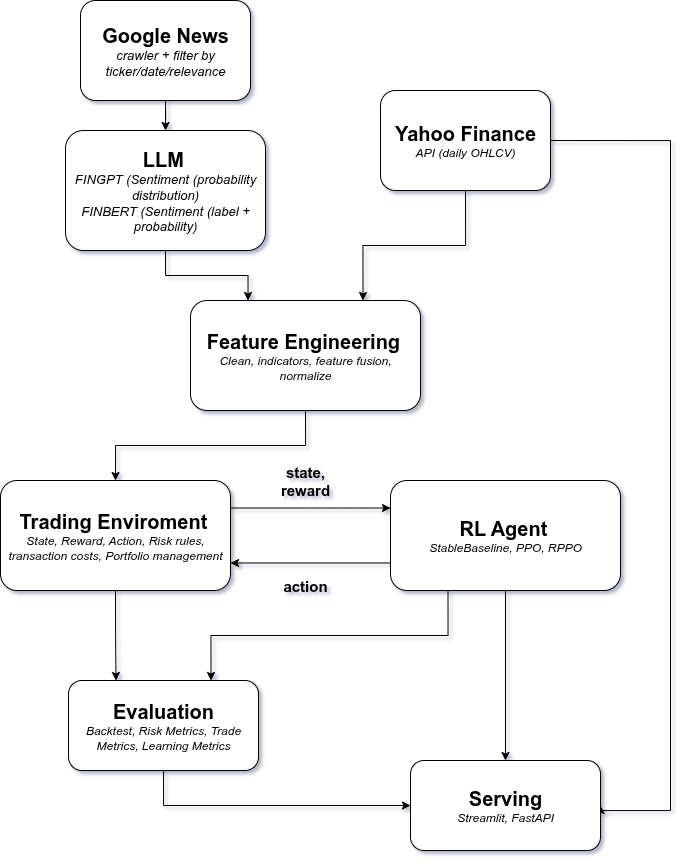
\includegraphics[width=\linewidth]{photos/finrlllm.drawio.png}
  \caption{معماری کلی سیستم}
  \label{fig:architecture}
\end{figure}

\paragraph{تعامل اجزا.}
\begin{enumerate}
    \item \textbf{گردآوری داده‌ها.} مقالات \lr{Google News} با استفاده از یک خزنده اختصاصی همراه با فیلتر نماد/تاریخ جمع‌آوری می‌شوند؛ داده‌های روزانه \lr{OHLCV} نیز از طریق \lr{API} در \lr{Yahoo Finance} دریافت می‌گردند. تمام داده‌ها در زمان \lr{UTC} برچسب‌گذاری و به نمادهای مربوطه نگاشت می‌شوند.
    
    \item \textbf{احساس مبتنی بر مدل‌های زبانی بزرگ.} هر مقاله یا تیتر به دو مدل ارسال می‌شود: \lr{FinGPT} یک توزیع احتمالی \(P(pos, neg, neu)\) تولید می‌کند؛ \lr{FinBERT} نیز توزیع مشابهی روی سه برچسب گزارش می‌کند. این سیگنال‌ها برای هر دارایی تجمیع و با داده‌های معاملاتی هم‌تراز می‌شوند.
    
    \item \textbf{پیش‌پردازش و ترکیب ویژگی‌ها.} داده‌ها یکتا‌سازی و پاک‌سازی می‌شوند، شاخص‌های فنی (\lr{EMA}، \lr{MACD}، \lr{RSI}، \lr{ATR}، \lr{Bollinger width}، تکانه/بازدهی) محاسبه و ویژگی‌ها نرمال‌سازی شده و در نهایت با \lr{OHLCV} و احساس ادغام می‌گردند.
    
\item \textbf{محیط.} محیطی مشابه \lr{Gym} تعریف شده است که حالت ترکیبی شامل وجه نقد، دارایی‌ها، شاخص‌های فنی، احساسات و شاخص‌های ریسک را در اختیار عامل قرار می‌دهد. همچنین محدودیت‌های عمل مانند وزن‌های \lr{softmax} با سقف تخصیص برای هر دارایی و ممنوعیت فروش استقراضی، هزینه‌های تراکنش (۰.۱\% برای خرید و فروش) و قوانین مدیریت ریسک (آشفتگی نرم و سخت) در آن اعمال می‌شوند.
    
\item \textbf{عامل یادگیری تقویتی.} عامل با استفاده از الگوریتم‌های \lr{PPO} و \lr{RPPO} (در بخش \lr{contrib} از \lr{Stable-Baselines3}) آموزش داده می‌شود.  
    
    \item \textbf{مدیریت سبد دارایی.} اعمال عامل به سفارش‌های صحیح سهام تبدیل شده، هزینه‌ها لحاظ شده و وضعیت سبد (وجه نقد/دارایی‌ها/سود و زیان) به‌روزرسانی می‌گردد.
    
    \item \textbf{ارزیابی.} روی مجموعه آزمون مجزا، ماژول ارزیابی مجدداً قیمت‌ها را از \lr{Yahoo Finance} واکشی کرده، معیارهای مالی \lr{Sharpe}، \lr{CAGR} و \lr{Max Drawdown} را محاسبه و با خط‌پایه‌ها (مانند فقط \lr{OHLCV} بدون احساس) مقایسه می‌کند.
    
    \item \textbf{ارائه.} نتایج و در صورت نیاز پیش‌بینی زنده از طریق داشبورد \lr{Streamlit} و سرویس \lr{FastAPI} در اختیار قرار می‌گیرند.
\end{enumerate}


\paragraph{منطق طراحی.}
دو کانال احساسی (احتمالات \lr{FinGPT} و \lr{FinBERT}) سیگنال‌های مکمل فراهم می‌کنند؛ 
ادغام آن‌ها با \lr{OHLCV} و شاخص‌های فنی، فضای حالت را غنی‌تر می‌سازد بدون آن‌که نشت اطلاعات آینده رخ دهد. 
اعمال کنترل‌های صریح آشفتگی و هزینه‌های تراکنش موجب واقع‌گرایی در پویایی آموزش می‌شوند. 
بخش ارزیابی داده‌های قیمتی را دوباره واکشی می‌کند تا جداسازی شفاف میان داده‌های آموزش و آزمون تضمین گردد. 
در نهایت، جداسازی بخش ارائه (\lr{Streamlit}/\lr{FastAPI}) از آموزش، امکان آزمایش‌های آفلاین بازتولیدپذیر و استقرار ماژولار را فراهم می‌سازد.


\section{توصیف بازار انتخاب‌شده}

در ابتدا، بازار رمزارزها به‌عنوان محیط هدف انتخاب شد و \lr{Bitcoin} به‌عنوان دارایی اصلی در نظر گرفته شد. 
روش‌های پایه‌ی یادگیری تقویتی روی این بازار پیاده‌سازی شدند و حتی تحلیل احساسات با استفاده از مدل‌های زبانی بزرگ نیز به آن اضافه گردید. 
با این حال، نتایج بهبود معناداری نشان ندادند. 
با بررسی‌های بیشتر دریافتم که بازار رمزارزها نوسان بسیار بالا و پیچیدگی زیادی دارد که دستیابی به نتایج پایدار و سازگار را دشوار می‌سازد. 
بنابراین تصمیم گرفتم تمرکز پژوهش را به بازار دیگری تغییر دهم.  

پس از انجام تحقیقات بیشتر، بازار سهام ایالات متحده و به‌طور مشخص شاخص \lr{Dow Jones Industrial Average (DOW30)} انتخاب شد. 
برای ساده‌سازی دامنه و کاهش پیچیدگی ناشی از کار با تعداد زیاد سهام، یک زیرمجموعه شامل چهار شرکت انتخاب شد: 
\lr{Apple (AAPL)}، \lr{JPMorgan Chase (JPM)}، \lr{Boeing (BA)} و \lr{Goldman Sachs (GS)}.  
این انتخاب به‌طور هدفمند انجام شد تا دو سهم با پوشش خبری فراوان (\lr{AAPL} و \lr{JPM}) و دو سهم با دسترسی محدودتر به اخبار (\lr{BA} و \lr{GS}) در بر گرفته شوند.  

علاوه بر این، تحلیل در این پروژه بر مبنای داده‌های \textbf{روزانه} انجام شد و از داده‌های با فرکانس بالاتر مانند ساعتی یا دقیقه‌ای استفاده نگردید. 
انتخاب داده‌های روزانه به دلایل زیر صورت گرفت:

\begin{enumerate}
    \item پردازش آن ساده‌تر و از نظر محاسباتی کم‌هزینه‌تر است.  
    \item اثر نویزهای کوتاه‌مدت و نوسانات شدید را کاهش می‌دهد.  
    \item نسبت به داده‌های با بسامد بالا در دسترس‌تر و قابل‌اعتمادتر است.  
    \item هم‌سویی بیشتری با منابع اطلاعاتی بیرونی مانند اخبار و تحلیل احساسات دارد که غالباً به‌صورت روزانه منتشر می‌شوند.  
    \item نتایج پایدارتر و قابل‌تفسیرتری برای ارزیابی راهبردهای معاملاتی فراهم می‌کند.  
\end{enumerate}

مراحل بعدی این پروژه با استفاده از این زیرمجموعه سهام به‌عنوان محیط اصلی انجام گرفت.  


\section{جمع‌آوری داده}

داده‌های موردنیاز این پروژه به دو دسته اصلی تقسیم می‌شوند:
\begin{itemize}
    \item \textbf{داده‌های فنی بازار}  
    \item \textbf{داده‌های مرتبط با اخبار}
\end{itemize}

برای داده‌های فنی، شاخص‌های استاندارد مالی مانند \lr{Open, Close, Low, High, Volume (OCLHV)}، شاخص نوسان \lr{(Volatility Index, VIX)} و شاخص آشفتگی \lr{(Turbulence Index)} گردآوری شدند. این مجموعه داده‌ها از \lr{Yahoo Finance} و با استفاده از کتابخانه‌های پایتون استخراج گردیدند که یک منبع رایگان، معتبر و دارای مستندات کافی برای اطلاعات بازار مالی محسوب می‌شود.  

بخش چالش‌برانگیزتر جمع‌آوری داده مربوط به اخبار مالی بود. دسترسی به منابع باکیفیت اخبار مالی اغلب مستلزم اشتراک‌های گران‌قیمت است و خزیدن در چنین وب‌سایت‌هایی معمولاً به دلیل تدابیر امنیتی و ضدبات با محدودیت مواجه می‌شود. در بازار رمزارزها، من از وب‌سایت \lr{https://cryptoslate.com/} استفاده کردم که امکان فیلترگذاری بر اساس رمزارزهای مختلف را فراهم می‌کرد. از طریق این منبع توانستم اخبار مرتبط با \lr{Bitcoin} را در بازه‌ای دوساله (از ابتدای 2024 تا 2025) استخراج کنم. این داده‌های استخراج‌شده به‌صورت عمومی در دسترس قرار گرفته‌اند (لینک اضافه خواهد شد).  

در مقابل، بازار سهام ایالات متحده چالش بزرگ‌تری ایجاد کرد، چراکه بیشتر رسانه‌های معتبر مالی محدودیت‌های سخت‌گیرانه‌تری داشتند و جمع‌آوری داده به‌صورت نظام‌مند را دشوار می‌ساختند. برای حل این مشکل، از \lr{Google News} استفاده شد که فیلترهای جست‌وجوی منعطفی برای نماد سهام، بازه زمانی و مرتب‌سازی بر اساس ارتباط یا اعتبار منبع ارائه می‌دهد. با این روش توانستم اخبار مرتبط با چهار شرکت منتخب (\lr{AAPL, JPM, BA, GS}) را در بازه 2010 تا 2025 جمع‌آوری کنم.  

مجموعه داده استخراج‌شده شامل فیلدهای زیر است: عنوان خبر، خلاصه، لینک، تاریخ انتشار، \lr{finbert\_label}، \lr{finbert\_score}، \lr{fingpt\_label} و \lr{fingpt\_score}. جزئیات مربوط به تولید این امتیازهای احساسی در بخش \textit{استخراج احساس از اخبار} توضیح داده خواهد شد.  

برای فرآیند \lr{web scraping} از کتابخانه \lr{Selenium} در پایتون استفاده شد که امکان مرور خودکار و استخراج داده از هر دو منبع \lr{CryptoSlate} و \lr{Google News} را فراهم ساخت. داده‌های پردازش‌شده نهایی ذخیره و به‌اشتراک گذاشته شده‌اند (لینک اضافه خواهد شد).  

\section{تحلیل داده}

تحلیل اصلی در این پروژه بر بررسی رابطه میان امتیازهای احساسی و تغییرات قیمتی بعدی در طول زمان متمرکز بود.
 
به‌طور خاص، بررسی شد که آیا احساس استخراج‌شده از اخبار می‌تواند به پیش‌بینی بازدهی‌های آتی سهام کمک کند یا خیر.  

برای این منظور از تحلیل علیت \lr{Granger} بر پایه مدل \lr{Vector Autoregression (VAR)} استفاده شد. 
آزمون \lr{Granger causality test} یک روش آماری است که تعیین می‌کند آیا یک سری زمانی می‌تواند اطلاعات پیش‌بینانه برای سری زمانی دیگر فراهم کند یا خیر. 
به عبارت دیگر، اگر وارد کردن مقادیر گذشته‌ی امتیاز احساس پیش‌بینی بازدهی سهام را نسبت به حالتی که تنها از بازدهی‌های گذشته استفاده شود بهبود دهد، آنگاه گفته می‌شود سری احساسی \lr{Granger-cause} بازدهی است. 
این رویکرد امکان آزمون هم‌زمان قدرت پیش‌بینی چندین ویژگی احساسی را با در نظر گرفتن وابستگی‌های با وقفه فراهم می‌سازد.  

پیش از انجام این تحلیل لازم است همه متغیرها ایستا باشند، یعنی خواص آماری آن‌ها (میانگین، واریانس) در طول زمان تغییر نکنند. 
برای دستیابی به ایستایی، تحلیل بر روی \textbf{بازدهی‌ها} (اختلاف لگاریتمی قیمت‌های پایانی متوالی) به‌جای قیمت‌های خام انجام شد. 
به‌طور مشابه، امتیازهای احساسی حاصل از \lr{FinBERT} و \lr{FinGPT} در سطح روزانه تجمیع شده و با استفاده از میانگین متحرک (با پنجره ۷ روزه و نیمه‌عمر \lr{۲.۵} روز) هموار شدند تا اثر اخبار طی چند روز بعدی بازتاب داده شود.  

ایستایی هر سری زمانی با آزمون \lr{Augmented Dickey-Fuller (ADF)} بررسی شد. 
این آزمون فرض صفر مبنی بر وجود ریشه واحد در سری (یعنی ناایستایی) را ارزیابی می‌کند. 
در صورت رد فرض صفر، سری ایستا محسوب شده و برای مدل‌سازی \lr{VAR} مناسب خواهد بود.  

با این روش، توانستم عملکرد پیش‌بینی امتیازهای احساسی \lr{FinBERT} و \lr{FinGPT} را در ارتباط با بازدهی‌های روزانه سهام مقایسه و ارزیابی کنم. 
روش‌شناسی دقیق استخراج این امتیازها از اخبار در بخش \textit{استخراج احساس از اخبار} تشریح خواهد شد. 
نتایج آزمون‌ها و ارزیابی‌های پیش‌بینانه در فصل \textit{آزمایش‌ها و نتایج} ارائه و بحث می‌شوند.  


\section{استخراج احساس از اخبار}
\label{sec:sentiment_extraction}

در این پروژه از دو مدل زبانی تخصصی در حوزه مالی برای تحلیل احساسات استفاده شده است: 
\textbf{\lr{FinBERT}} و \textbf{\lr{FinGPT}}. 
هر دو مدل یک توزیع احتمالی روی برچسب‌های \lr{positive}، \lr{negative} و \lr{neutral} ارائه می‌کنند، 
اما از نظر معماری، تعداد پارامترها، داده‌های آموزش‌دیده و پیچیدگی در مرحله استنتاج، تفاوت‌های قابل توجهی با یکدیگر دارند.  

\subsection{\lr{FinBERT}}
\label{subsec:finbert}
\textbf{\lr{FinBERT}} یک \lr{Transformer} از نوع فقط رمزگذار است که بر پایه \lr{BERT-base} ساخته شده 
و برای حوزه مالی بازآموزی شده است. 
این مدل از پیکربندی استاندارد \lr{BERT} 
(۱۲ لایه، ۱۲ سر توجه، اندازه بردار پنهان 768 و حدود ۱۱۰ میلیون پارامتر) استفاده می‌کند.  
\lr{FinBERT} ابتدا با متون مالی در مقیاس بزرگ پیش‌تمرین داده شده 
و سپس روی مجموعه‌داده‌های برچسب‌خورده‌ای مانند \lr{Financial PhraseBank} برای طبقه‌بندی احساس ریزتنظیم شده است.  
در نسخه عمومی \lr{\texttt{ProsusAI/finbert}}، لایه نهایی یک توزیع \lr{softmax} 
روی سه برچسب \lr{positive}، \lr{negative} و \lr{neutral} تولید می‌کند \cite{araci2019finbert}.  

\subsection{\lr{FinGPT (Llama~3 + LoRA adapters)}}
\label{subsec:fingpt}
\lr{FinGPT} یک مدل زبانی بزرگ از نوع فقط رمزگذار است که بر پایه \lr{\texttt{meta-llama/Meta-Llama-3-8B}} ساخته شده 
و با استفاده از \lr{LoRA adapters} و ریزتنظیم مبتنی بر دستورالعمل برای حوزه مالی سازگار گردیده است.  
مدل \lr{\texttt{FinGPT/fingpt-mt\_llama3-8b\_lora}} ماژول‌های سبک \lr{LoRA} را به مدل پایه متصل می‌کند 
و این امکان را فراهم می‌سازد که تنها با تعداد کمی پارامتر قابل‌آموزش، انطباق دامنه‌ای انجام شود.  
ابتکار \lr{FinGPT} یک رویکرد داده‌محور دارد: گردآوری خودکار داده‌های مالی 
(مانند اخبار، گزارش‌ها، شبکه‌های اجتماعی و جفت‌های پرسش‌وپاسخ) و سپس سازگاری مدل‌های بازمتن.  
برای تحلیل احساس، \lr{FinGPT} آموزش دیده است که دستورالعمل‌ها را دنبال کند 
و یکی از برچسب‌های \lr{positive}، \lr{negative} یا \lr{neutral} را تولید نماید \cite{yang2023fingpt}.  

\subsection{امتیازدهی عددی احساسات}
برای هر دو مدل، خروجی خام یک توزیع احتمالی روی سه کلاس احساسی است.  
برای تبدیل این توزیع به یک امتیاز عددی منفرد، یک رویکرد ساده و کارآمد به‌کار گرفته شد:  
اختلاف میان احتمال پیش‌بینی‌شده کلاس‌های \lr{positive} و \lr{negative}.  
به‌صورت رسمی:
\[
Sentiment Score = P(positive) - P(negative).
\]
این تعریف تضمین می‌کند که امتیازهای بالاتر نشان‌دهنده احساس مثبت‌تر، 
امتیازهای پایین‌تر بیانگر احساس منفی‌تر و مقادیر نزدیک به صفر معادل با حالت خنثی خواهند بود.  



\section{محیط معاملاتی}
\label{sec:rl_env}


\subsection{محیط معاملاتی سفارشی‌سازی‌شده}
به‌عنوان نقطه آغاز، از محیط متن‌باز موجود در کتابخانه \lr{FinRL}\LTRfootnote{\url{https://github.com/AI4Finance-Foundation/FinRL/blob/master/finrl/meta/env_stock_trading/env_stocktrading.py}} استفاده شد.  
به دلیل متن‌باز بودن، این محیط به‌طور گسترده سفارشی‌سازی گردید.  
اصلاحات اصلی شامل موارد زیر بودند:
\begin{itemize}
    \item طراحی مجدد \textbf{فضای حالت} با افزودن ویژگی‌های فنی، احساسی و ریسکی.  
    \item بازتعریف \textbf{تابع پاداش} برای بازتاب بهتر عملکرد سبد سهام.  
    \item پیاده‌سازی یک \textbf{سازوکار کنترل ریسک} مبتنی بر آشفتگی بازار.  
    \item پشتیبانی از \textbf{آموزش چندمحیطی} به‌منظور بهبود پایداری.  
    \item \textbf{تصادفی‌سازی دوره‌ها} با تاریخ‌های شروع و طول‌های متغیر.  
    \item یک \textbf{سازوکار اجرای عمل جدید} بر پایه وزن‌های سبد سهام.  
\end{itemize}

\subsection{فضای حالت}
نمایش نهایی حالت شامل ادغام شاخص‌های فنی، معیارهای ریسک، سیگنال‌های احساسی و اطلاعات سبد سهام است.  
هر ویژگی استانداردسازی می‌شود تا قابلیت مقایسه بین سهام مختلف فراهم گردد.  
شاخص‌های فنی با استفاده از کتابخانه متن‌باز \lr{ta}\LTRfootnote{\url{https://github.com/bukosabino/ta}} محاسبه شدند 
که پیاده‌سازی کارآمدی از شاخص‌های فنی استاندارد بازار ارائه می‌دهد.  

مجموعه کامل ویژگی‌ها عبارت است از:
\begin{itemize}
    \item \textbf{\lr{20-day momentum (mom\_20d)}:} تغییر نسبی قیمت طی ۲۰ روز گذشته برای ثبت تکانه کوتاه‌مدت.  
    \item \textbf{\lr{Exponential Moving Averages (ema\_20, ema\_60)}:} روندهای قیمتی کوتاه‌مدت و میان‌مدت.  
    \item \textbf{\lr{MACD} و \lr{signal line}:} شاخص‌های تکانه برای شناسایی تغییر روند.  
    \item \textbf{\lr{Relative Strength Index (RSI, 14-day)}:} نوسانگر برای تشخیص شرایط اشباع خرید یا فروش.  
    \item \textbf{\lr{Average True Range (ATR, 14-day)}:} معیاری از نوسان بازار بر اساس دامنه‌های معاملاتی.  
    \item \textbf{\lr{Bollinger Band Width}:} شاخص نوسان مبتنی بر فاصله میان باندهای بولینگر.  
    \item \textbf{\lr{Normalized closing price (zclose\_60)}:} قیمت پایانی نرمال‌شده نسبت به پنجره ۶۰ روزه.  
    \item \textbf{\lr{Daily return (ret\_1d)}:} بازدهی یک‌روزه برای سنجش عملکرد کوتاه‌مدت دارایی.  
    \item \textbf{\lr{Sentiment scores (finbert\_future, fingpt\_future)}:} امتیازهای احساسی استخراج‌شده از اخبار مالی توسط \lr{FinBERT} و \lr{FinGPT}.  
    \item \textbf{\lr{On-Balance Volume (OBV)}:} شاخص مبتنی بر حجم برای نشان‌دادن جریان سرمایه.  
    \item \textbf{\lr{Normalized VIX}:} شاخص نوسان بازار به‌عنوان نماینده ریسک سیستماتیک.  
    \item \textbf{\lr{Portfolio state}:} تعداد نرمال‌شده سهام هر دارایی و موجودی نقدی نرمال‌شده.  
\end{itemize}


\subsection{تابع پاداش}
در این کار از دو تعریف ساده برای پاداش استفاده شده است:

\begin{enumerate}
    \item \textbf{بازدهی خام نرمال‌شده سبد سهام در طول دوره (\lr{episode-normalized return}).}
    در این روش تغییرِ ارزش سبد سهام نسبت به ابتدای دوره محاسبه و متناسب با طول دوره مقیاس‌دهی می‌شود:
    \[
    R^{\text{ep}} \;=\; 
    \frac{A_{end} - A_{begin}}{A_{begin} + \varepsilon}
    \;\times\;
    \frac{n_{days}}{L}
    \;\times\;
    \kappa,
    \]
    که در آن \(A_{begin}\) و \(A_{end}\) به‌ترتیب ارزش سبد سهام در آغاز و پایان دوره هستند، 
    \(L\) طول دوره (به تعداد روز/گام)، \(n_{days}\) ضریب نرمال‌سازی زمانی، 
    \(\kappa\) ثابت \lr{reward scaling} و \(\varepsilon\) یک مقدار کوچک برای پایداری عددی است.
    \vspace{0.25em}

    \item \textbf{بازدهی لگاریتمی تعدیل شده (\lr{one-step log return}).}
    در این روش پاداش هر گام زمانی بر اساس بازدهی لحظه‌ای سبد سهام تعریف می‌شود و برای ریسک‌گریزی، از لگاریتم استفاده می‌گردد:
    \[
    r_t \;=\; \log\!\big( \max(10^{-3},\, 1 + \rho_t) \big)\; \times\; \kappa,
    \qquad
    \rho_t \;=\; \frac{A_t - A_{t-1}}{A_{t-1} + \varepsilon},
    \]
    که در آن \(A_t\) ارزش سبد سهام در انتهای گام \(t\) است. 
    در گام نخست، اگر \(A_{t-1}\) در دسترس نباشد، بازدهی یک‌گام به‌صورت امن مقداردهی می‌شود تا از ناپایداری عددی جلوگیری گردد.
\end{enumerate}



\subsection{کنترل ریسک با استفاده از آشفتگی}
برای مدیریت ریسک در دوره‌های پرنوسان، یک سازوکار مبتنی بر آشفتگی به‌کار گرفته شد.  
آشفتگی شرایط غیرعادی بازار را از طریق مقایسه حرکات قیمتی با کوواریانس تاریخی کمی‌سازی می‌کند.  
دو آستانه در نظر گرفته شد:
\begin{itemize}
    \item \textbf{آستانه نرم} ($\tau_{soft} = 70$): در صورت عبور، هیچ دستور خرید جدیدی اجرا نمی‌شود.  
    \item \textbf{آستانه سخت} ($\tau_{hard} = 100$): در صورت عبور، همه موقعیت‌های موجود نقد می‌شوند و خریدهای بعدی مسدود می‌گردند.  
\end{itemize}

این سازوکار باعث می‌شود عامل در شرایط بحرانی رفتار محافظه‌کارانه‌تری داشته باشد.  

\subsection{تصادفی‌سازی دوره}
محیط پیش‌فرض \lr{FinRL} دوره‌‌ها را به‌صورت بازه‌های ثابت تعریف می‌کند که از نخستین روز معاملاتی آغاز شده و در آخرین روز داده‌ها پایان می‌یابند.  
اگرچه این رویکرد یک ساختار آموزشی سازگار فراهم می‌کند، اما تنوع شرایط بازاری تجربه‌شده توسط عامل را محدود می‌سازد.  
برای رفع این محدودیت، \textbf{تصادفی‌سازی دوره‌ها} معرفی گردید.  

به‌صورت رسمی، فرض کنید $T$ تعداد کل روزهای معاملاتی در مجموعه داده و $L_{\min}$ حداقل طول مجاز دوره باشد.  
در ابتدای هر دوره، یک روز شروع $s$ به‌صورت تصادفی از توزیع یکنواخت انتخاب می‌شود:
\[
s \sim Uniform(0, T - L_{\min}).
\]
سپس طول دوره $L$ از بازه زیر نمونه‌گیری می‌شود:
\[
L \sim Uniform(L_{\min}, T - s).
\]
دور از $s$ تا $s + L$ ادامه می‌یابد تا قید حداقل طول رعایت شود.  
با احتمال کم، کل مجموعه داده مورد استفاده قرار می‌گیرد ($s=0$, $L=T$) تا سازگاری با تنظیمات اولیه حفظ شود.  

این استراتژی تنوع بیشتری در زیر‌بازه‌های بازار به عامل معرفی می‌کند و باعث بهبود تعمیم با:
\begin{itemize}
    \item جلوگیری از بیش‌برازش روی الگوهای زمانی خاص.  
    \item شبیه‌سازی شرایط آموزشی نزدیک‌تر به معامله‌گری واقعی، که تاریخ شروع و افق زمانی متغیر هستند.  
    \item افزایش مقاومت در برابر رژیم‌های متفاوت نوسان و چرخه‌های بازار.  
\end{itemize}

\subsection{سازوکار اجرای عمل}

در پیاده‌سازی پیش‌فرض \lr{FinRL}، عمل برای هر سهم $i$ یک \textbf{عدد منفرد} 
$a_i \in [-1,1]$ است که در یک ثابت $h_{\max}$ ضرب می‌شود تا تعداد سهام خریداری یا فروخته‌شده تعیین گردد.  
این شیوه چند محدودیت جدی دارد:
\begin{itemize}
    \item با ارزش کل \textbf{سبد سهام} مقیاس‌پذیر نیست.  
    \item تفاوت قیمت سهام را در نظر نمی‌گیرد.  
    \item عامل را به حجم‌های ثابت معامله محدود می‌کند، بدون توجه به شرایط بازار.  
\end{itemize}

برای رفع این محدودیت‌ها، عمل به‌صورت یک \textbf{مسئله تخصیص سبد سهام} بازنویسی شد.  
بردار اولیه اعمال به‌صورت $\mathbf{z} \in \mathbb{R}^N$ (به‌همراه یک مؤلفه مربوط به وجه نقد) تعریف می‌شود.  
سپس این مقادیر به وزن‌های نرمال‌شده $\mathbf{w}$ با استفاده از تبدیل \lr{softmax} تبدیل می‌گردند:
\[
w_i = \frac{\exp(z_i)}{\sum_{j=1}^{N+1} \exp(z_j)}, \quad i=1,\dots,N+1,
\]
به‌طوری که $\sum_{i=1}^{N+1} w_i = 1$.  

برای جلوگیری از تمرکز بیش‌ازحد روی یک دارایی خاص، سقف تخصیص اعمال می‌شود:
\[
w_i^{capped} = \min(w_i, \, c), \quad c=0.5.
\]

بر این اساس، مقدار هدف برای سرمایه‌گذاری در سهم $i$ به‌صورت زیر محاسبه می‌شود:
\[
d_{i,t} = w_i^{capped} \cdot A_t,
\]
که در آن $A_t$ ارزش فعلی \textbf{سبد سهام} است.  
تعداد سهام هدف نیز به‌صورت زیر تعیین می‌گردد:
\[
q_{i,t}^{target} = \left\lfloor \frac{d_{i,t}}{p_{i,t}} \right\rfloor,
\]
که در آن $p_{i,t}$ قیمت سهم در زمان $t$ است.  
اختلاف با وضعیت فعلی حجم معامله لازم را مشخص می‌کند:
\[
\Delta q_{i,t} = q_{i,t}^{target} - q_{i,t}^{current}.
\]

پس از آن، آستانه‌های آشفتگی (بخش~\ref{sec:rl_env}) اعمال می‌شوند:
\begin{itemize}
    \item اگر آشفتگی $> \tau_{hard}$ باشد: همه $q_{i,t}$ برابر صفر می‌شوند (تصفیه کامل).  
    \item اگر $\tau_{soft} < \text{آشفتگی} \leq \tau_{hard}$: هیچ دستور خریدی اجرا نمی‌شود و تنها فروش مجاز است، یعنی $\Delta q_{i,t} = \min(0, \Delta q_{i,t})$.  
\end{itemize}

این بازنویسی چند مزیت کلیدی دارد:
\begin{itemize}
    \item اعمال متناسب با ارزش سبد سهام و قیمت دارایی‌ها مقیاس می‌شوند.  
    \item عامل به‌جای انتخاب تعداد دلخواه سهام، یک راهبرد تخصیص بهینه می‌آموزد.  
    \item ریسک به‌طور مستقیم با استفاده از سقف تخصیص و کنترل آشفتگی مدیریت می‌شود.  
\end{itemize}

\subsection{جمع‌بندی}
محیط سفارشی‌شده در این پروژه دارای مزایای زیر است:
\begin{itemize}
    \item نمایش حالت جامع و پرجزئیات با ترکیب داده‌های فنی، احساسی و ریسک.  
    \item تعریف توابع پاداش که مستقیماً با عملکرد \textbf{سبد سهام} ارتباط دارند.  
    \item مدیریت ریسک شفاف و مؤثر بر پایه شاخص آشفتگی بازار.  
    \item افزایش تنوع آموزشی از طریق تصادفی‌سازی دوره‌ها و شرایط شروع.  
    \item سازوکار اجرای عمل پایدار و انعطاف‌پذیر بر مبنای وزن‌های سبد سهام.  
\end{itemize}

برای پیاده‌سازی از کتابخانه \lr{Gymnasium} استفاده شد که یکپارچگی کامل با اغلب عامل‌ها و چارچوب‌های یادگیری تقویتی را امکان‌پذیر می‌سازد و سازگاری کامل با محیط معاملاتی سفارشی تضمین می‌کند.  

\section{عامل یادگیری تقویتی}
\label{sec:rl_agent}

برای پیاده‌سازی عامل یادگیری تقویتی از کتابخانه \lr{Stable-Baselines3 (SB3)}\LTRfootnote{\url{https://github.com/DLR-RM/stable-baselines3}} و توسعه آن \lr{sb3-contrib} استفاده شد.  
این کتابخانه‌ها پیاده‌سازی‌های قابل‌اعتماد از الگوریتم‌های یادگیری تقویتی را ارائه داده و تعامل کامل با چارچوب \lr{Gymnasium} را فراهم می‌کنند، در نتیجه سازگاری کامل با محیط معاملاتی سفارشی تضمین می‌شود.  

\subsection{چارچوب پیاده‌سازی}
برای عامل یک \textbf{پوسته‌ی نرم‌افزاری} (\lr{wrapper}) اختصاصی طراحی شد تا اجرای آزمایش‌ها با الگوریتم‌های مختلف ساده‌تر شود.  
این پوسته امکانات اصلی زیر را فراهم می‌کند:
\begin{itemize}
    \item \textbf{مقداردهی مدل:} بارگذاری مدل‌های یادگیری تقویتی با استفاده از ابرپارامترهای پیش‌فرض یا تنظیم‌شده توسط کاربر.  
    \item \textbf{آموزش:} اجرای فرآیند آموزش همراه با ثبت گزارش‌ها و استفاده از مکانیزم‌های بازخوانی (\lr{callback}) برای پایش روند یادگیری.  
    \item \textbf{پیش‌بینی:} اجرای مدل روی داده‌های بازار جدید (که در آموزش استفاده نشده‌اند) و ثبت تغییرات سبد سهام و معاملات انجام‌شده.  
\end{itemize}

\subsection{الگوریتم‌های ارزیابی‌شده}
چندین الگوریتم یادگیری تقویتی از \lr{SB3} و \lr{sb3-contrib} روی مجموعه داده اعتبارسنجی ارزیابی شدند، از جمله:
\begin{itemize}
    \item \lr{A2C}، \lr{PPO}، \lr{SAC}، \lr{TD3} (از \lr{SB3})  
    \item \lr{RecurrentPPO}، \lr{CrossQ}، \lr{TRPO} (از \lr{sb3-contrib})  
\end{itemize}

از میان این الگوریتم‌ها، دو مورد بر اساس عملکرد در اعتبارسنجی برای آزمایش‌های نهایی انتخاب شدند:  
\lr{Proximal Policy Optimization (PPO)} و \lr{Recurrent Proximal Policy Optimization (RecurrentPPO)}.  

\paragraph{\lr{PPO}.}
 یک روش مبتنی بر گرادیان سیاست است که با محدودسازی به‌روزرسانی‌های سیاست از طریق تابع هدف برش‌یافته (\lr{clipped surrogate objective})، آموزش را پایدار می‌سازد.  
این امر از به‌روزرسانی‌های بیش‌ازحد بزرگ جلوگیری کرده و تعادلی میان اکتشاف و بهره‌برداری برقرار می‌کند.  
به دلیل سادگی و پایداری، \lr{PPO} به یکی از پرکاربردترین الگوریتم‌ها در مسائل کنترل پیوسته از جمله معامله‌گری مالی تبدیل شده است.  




\paragraph{\lr{RecurrentPPO}.}
 چارچوب \lr{PPO} را با افزودن شبکه‌های عصبی بازگشتی (مانند \lr{LSTM}) به معماری سیاست گسترش می‌دهد.  
این ارتقاء به عامل امکان می‌دهد وابستگی‌های زمانی را ثبت کرده و اطلاعات حالت‌های گذشته را حفظ کند، 
که در بازارهای مالی بسیار سودمند است زیرا زمینه تاریخی و الگوهای سری‌های زمانی در تصمیم‌گیری نقش دارند.  

\subsection{بهینه‌سازی ابرپارامترها}
عملکرد الگوریتم‌های یادگیری تقویتی به‌شدت به انتخاب ابرپارامترها (مانند نرخ یادگیری، ضریب تنزیل، اندازه دسته و بازه برش) حساس است.  
برای تنظیم نظام‌مند این پارامترها، از کتابخانه \lr{Optuna}\LTRfootnote{\url{https://optuna.org/}} استفاده شد.  
جست‌وجوی ابرپارامترها روی مجموعه اعتبارسنجی انجام گرفت تا پیکربندی‌های مقاوم به‌دست آید و از بیش‌برازش جلوگیری شود.  

ابرپارامترهای بهینه و نتایج متناظر آن‌ها در فصل \textit{آزمایش‌ها و نتایج} گزارش خواهند شد.  

\section{پایش}
\label{sec:monitoring}

پایش یکی از مؤلفه‌های کلیدی در آموزش و ارزیابی مدل‌های یادگیری تقویتی است، 
به‌ویژه در حوزه مالی که عملکرد مدل‌ها به‌شدت به ابرپارامترها و شرایط متغیر بازار وابسته است.  
برای این منظور، یک چارچوب پایش بهبودیافته طراحی شد که قابلیت‌های پایه موجود در کتابخانه \lr{FinRL} را گسترش می‌دهد.  

\subsection{رویکرد}
پیشرفت فرایند آموزش با استفاده از مکانیزم‌های \textbf{بازخوانی} (\lr{callback}) دنبال شد.  
این مکانیزم‌ها سیگنال‌های کلیدی مانند پاداش‌ها، طول دوره‌ها و نرخ‌های یادگیری را ثبت می‌کنند.  
سپس این داده‌ها با ابزارهای بصری‌سازی مانند \lr{TensorBoard} و \lr{Weights \& Biases (W\&B)} یکپارچه شدند 
تا امکان بررسی بلادرنگ روند یادگیری فراهم گردد.  
در مقایسه با پیکربندی پیش‌فرض، این چارچوب پایش بهبودیافته دید دقیق‌تر و قابل‌اعتمادتری از رفتار مدل در طول آموزش ارائه می‌دهد.  

\subsection{مزایا}
این چارچوب پایش امکانات زیر را فراهم کرد:
\begin{itemize}
    \item شناسایی زودهنگام بی‌ثباتی یا واگرایی در روند آموزش.  
    \item مقایسه منظم و دقیق الگوریتم‌ها و پیکربندی‌های مختلف ابرپارامتر.  
    \item ارزیابی شفاف‌تر عملکرد مدل در مراحل گوناگون آموزش و اعتبارسنجی.  
\end{itemize}


\section{ارائه و استقرار}
\label{sec:deployment}

برای استفاده عملی از مدل‌های آموزش‌دیده یادگیری تقویتی، یک پایپلاین ارائه و استقرار طراحی شد.  
این سیستم از دو بخش اصلی تشکیل شده است:  
\begin{itemize}
    \item \textbf{بخش  (\lr{Backend}):} پیاده‌سازی‌شده با \lr{FastAPI}، مسئول اجرای مدل و پاسخ به درخواست‌ها.  
    \item \textbf{بخش  (\lr{Frontend}):} ساخته‌شده با \lr{Streamlit}، برای نمایش نتایج و تعامل ساده با کاربر.  
\end{itemize}

\subsection{بخش \lr{Backend}}
این بخش مدل‌های آموزش‌دیده را بارگذاری کرده و از طریق رابط‌های برنامه‌نویسی کاربردی (\lr{API}) در دسترس قرار می‌دهد.  
وظایف اصلی آن عبارت‌اند از:
\begin{itemize}
    \item اجرای مدل: دریافت داده ورودی و بازگرداندن تصمیم‌های معاملاتی پیشنهادی.  
    \item مدیریت سبد سهام: واکشی و نمایش موقعیت‌های باز و بسته.  
    \item آماده‌سازی داده: هماهنگ کردن داده‌های ورودی با قالب مورد انتظار مدل.  
\end{itemize}

\subsection{بخش \lr{Frontend}}
این بخش یک رابط تعاملی و ساده برای کاربران فراهم می‌کند و شامل سه قسمت اصلی است:
\begin{enumerate}
    \item \textbf{نمودار قیمت:} نمایش قیمت پایانی هر سهم در بازه انتخاب‌شده.  
    \item \textbf{تحلیل فنی:} محاسبه و نمایش شاخص‌ها و ویژگی‌های فنی منتخب.  
    \item \textbf{اقدامات معاملاتی:} نمایش خرید و فروش‌های پیشنهادی عامل در بازه انتخاب‌شده.  
\end{enumerate}

\subsection{جمع‌بندی}
این چارچوب امکان استفاده کامل از عامل معاملاتی را فراهم می‌کند.  
بخش پشتی مسئول اجرای مدل و پاسخگویی به درخواست‌هاست، در حالی‌که بخش کاربری نتایج را به‌صورت تصویری و قابل‌فهم برای کاربر نمایش می‌دهد.  


\section{جمع‌بندی}

در این فصل، تمامی اجزای اصلی پروژه از گردآوری داده تا استقرار نهایی شرح داده شدند.  
معماری کلی سیستم، انتخاب بازار و داده‌ها، طراحی محیط و عامل یادگیری تقویتی و همچنین فرآیند پایش و ارائه بررسی شدند.  
این مجموعه عناصر، چارچوبی منسجم و بازتولیدپذیر برای آزمون و ارزیابی راهبردهای معاملاتی مبتنی بر یادگیری تقویتی فراهم ساختند و زمینه لازم برای ارائه نتایج در فصل بعدی را مهیا کردند.  



\chapter{پیاده‌سازی}

\section{مقدمه}

این فصل جزئیات پیاده‌سازی سامانه پیشنهادی را ارائه می‌دهد.  
ابتدا ابزارها و کتابخانه‌های اصلی معرفی می‌شوند، سپس روش‌های تضمین بازتولیدپذیری نتایج و منابع محاسباتی مورد استفاده تشریح خواهند شد.  
در پایان نیز پیکربندی محاسباتی و تنظیمات اصلی آموزش بیان می‌شود تا ارتباط میان مباحث نظری و نتایج تجربی برقرار گردد.  


\section{ابزارها و چارچوب‌ها}

پیاده‌سازی پروژه در \lr{Python 3} انجام شد که یک چارچوب غنی برای علم داده، یادگیری تقویتی و استقرار فراهم می‌کند.  
جدول~\ref{tab:tools_frameworks} ابزارها و کتابخانه‌های اصلی مورد استفاده را نشان می‌دهد که بر اساس کارکرد گروه‌بندی شده‌اند.  

\begin{table}[H]
\centering
\renewcommand{\arraystretch}{1.3} % فاصله ردیف‌ها بیشتر
\begin{tabular}{p{4cm} p{10cm}}
\hline
\textbf{دسته‌بندی} & \textbf{ابزارها و کاربرد} \\
\hline

\textbf{گردآوری داده} 
 & \lr{yfinance} \lr{--} دریافت داده‌های \lr{OHLCV} از \lr{Yahoo Finance API}. \\
 & \lr{Selenium} \lr{--} جمع‌آوری اخبار \lr{Google News} با فیلتر نماد/تاریخ/ارتباط. \\[0.5em]

\textbf{پردازش داده و ویژگی‌ها} 
 & \lr{pandas}، \lr{numpy} \lr{--} پردازش، پاک‌سازی و نرمال‌سازی داده‌ها. \\
 & \lr{ta} \lr{--} محاسبه شاخص‌های فنی (\lr{EMA}، \lr{MACD}، \lr{RSI}، \lr{ATR}، \lr{Bollinger}). \\
 & \lr{json} \lr{--} ذخیره‌سازی تنظیمات و نتایج. \\[0.5em]

\textbf{محیط} 
 & \lr{gymnasium} \lr{--} رابط پایه محیط‌های یادگیری تقویتی. \\
 & \lr{FinRL} \lr{--} نمونه‌سازی سریع و سفارشی‌سازی محیط‌های معاملاتی. \\[0.5em]

\textbf{یادگیری تقویتی} 
 & \lr{stable\_baselines3} \lr{--} پیاده‌سازی الگوریتم‌هایی مانند \lr{PPO}، \lr{A2C}، \lr{DQN}. \\
 & \lr{sb3-contrib} \lr{--} توسعه \lr{RPPO}. \\
 & \lr{torch} \lr{--} موتور یادگیری عمیق برای آموزش مدل و ذخیره‌سازی نقاط وارسی. \\[0.5em]

\textbf{بهینه‌سازی ابرپارامترها} 
 & \lr{Optuna} \lr{--} تنظیم خودکار ابرپارامترها بر داده اعتبارسنجی. \\[0.5em]

\textbf{ردیابی آزمایش‌ها} 
 & \lr{wandb (Weights \& Biases)} \lr{--} ثبت، مصورسازی و مقایسه آزمایش‌ها. \\[0.5em]

\textbf{ارزیابی و مقایسه} 
 & \lr{scipy} \lr{--} ابزارهای عددی برای ارزیابی. \\
 & \lr{PyPortfolioOpt (pypfopt)} \lr{--} خط‌مبنای بهینه‌سازی میانگین-واریانس. \\[0.5em]

\textbf{مصورسازی} 
 & \lr{matplotlib}، \lr{seaborn} \lr{--} ترسیم نمودارهای ایستا از عملکرد. \\
 & \lr{plotly} \lr{--} نمودارهای تعاملی از منحنی سرمایه و تخصیص سبد سهام. \\[0.5em]

\textbf{استقرار و ارائه} 
 & \lr{Streamlit} \lr{--} رابط داشبوردی. \\
 & \lr{FastAPI} \lr{--} \lr{REST API} برای ارائه مدل. \\
 & \lr{requests} \lr{--} ارتباط با \lr{API}. \\
 & \lr{gdown} \lr{--} تبادل مدل‌ها/داده‌ها با \lr{Google Drive}. \\[0.5em]

\textbf{ابزار کمکی} 
 & \lr{Python logging} \lr{--} ثبت و مدیریت گزارش‌ها برای بازتولیدپذیری. \\

\hline
\end{tabular}
\caption{خلاصه ابزارها و چارچوب‌های مورد استفاده در پیاده‌سازی.}
\label{tab:tools_frameworks}
\end{table}


به‌طور کلی، این مجموعه ابزارها یک زنجیره کامل برای توسعه، آموزش، ارزیابی و استقرار سامانه معاملاتی فراهم کرده است.  
ابزار \lr{FinRL} امکان \textbf{نمونه‌سازی سریع} و ایجاد محیط‌های معاملاتی استاندارد را فراهم می‌کند.  
کتابخانه‌های \lr{Stable-Baselines3} و \lr{PyTorch} ستون اصلی برای \textbf{آموزش پایدار الگوریتم‌های یادگیری تقویتی} هستند که با استفاده از آن‌ها می‌توان مدل‌هایی مانند \lr{PPO} و \lr{RPPO} را به‌صورت قابل اعتماد پیاده‌سازی و اجرا کرد.  

برای \textbf{گردآوری خودکار داده‌ها}، از \lr{yfinance} برای دریافت داده‌های مالی \lr{OHLCV} و از \lr{Selenium} برای جمع‌آوری اخبار مالی (مانند \lr{Google News}) استفاده شد.  
این داده‌ها سپس توسط کتابخانه‌هایی مانند \lr{pandas} و \lr{numpy} پردازش و آماده‌سازی شدند و اندیکاتورهای فنی با کمک \lr{ta} محاسبه گردیدند.  

ابزار \lr{wandb} نقش کلیدی در \textbf{ردیابی دقیق آزمایش‌ها} ایفا کرد و امکان ثبت نمودارها، مقایسه نسخه‌های مختلف مدل و مدیریت سوابق آزمایش‌ها را فراهم آورد.  
همچنین برای \textbf{بهینه‌سازی خودکار ابرپارامترها} از \lr{Optuna} استفاده شد تا کارایی مدل‌ها در داده‌های اعتبارسنجی افزایش یابد.  

در نهایت، برای \textbf{استقرار عملی}، از \lr{Streamlit} به‌عنوان رابط کاربری داشبوردی برای نمایش نتایج و از \lr{FastAPI} به‌عنوان سرویس پشتی برای ارائه مدل‌ها و پاسخ به درخواست‌ها استفاده شد.  
ابزارهایی مانند \lr{requests} و \lr{gdown} نیز برای برقراری ارتباط با \lr{API} و تبادل مدل‌ها/داده‌ها با \lr{Google Drive} به‌کار گرفته شدند.  

این ترکیب از ابزارها و چارچوب‌ها باعث شد چرخه کامل \textbf{از جمع‌آوری داده تا استقرار نهایی عامل معاملاتی} به‌صورت منسجم، بازتولیدپذیر و کارآمد پیاده‌سازی شود.  

\section{بازتولیدپذیری و محیط}

آزمایش‌ها با استفاده از \lr{Python}، همراه با \lr{PyTorch} و \lr{Stable-Baselines3} اجرا شدند.  
محیط محاسباتی از پردازنده گرافیکی (\lr{GPU}) پشتیبانی می‌کرد.  

از آن‌جا که \lr{seed}های تصادفی در همه کتابخانه‌ها به‌طور کامل ثابت نشده بودند، 
نتایج اجرای تکی می‌توانند به دلیل عوامل تصادفی در یادگیری تقویتی 
(مانند مقداردهی اولیه مدل، فرآیند اکتشاف و تفاوت‌های سخت‌افزاری در \lr{GPU}) کمی متفاوت باشند.  
برای کاهش این مشکل، هر آزمایش چند بار تکرار شد و میانگین نتایج در ۱۰ اجرا گزارش شد 
تا نتایج قابل اعتمادتر باشند.  

برای تضمین بازتولیدپذیری داده‌ها، تاریخ دقیق دریافت داده‌های \lr{Yahoo Finance} ثبت شد 
و زمان جمع‌آوری تمام اخبار \lr{Google News} ذخیره گردید.  
همه زمان‌ها به \lr{UTC} تبدیل شدند و در فرآیند مهندسی ویژگی‌ها از هرگونه \textbf{نگاه به آینده} اجتناب شد.  

\section{سخت‌افزار و منابع محاسباتی}

آزمایش‌ها با ترکیبی از منابع ابری برای آموزش و استنتاج،  
و یک لپ‌تاپ محلی برای استقرار و تست سبک انجام شدند.  

\paragraph{\lr{Kaggle} (آموزش).}
بخش اصلی آموزش یادگیری تقویتی در محیط نوت‌بوک \lr{Kaggle} انجام شد.  
این محیط مجهز به \lr{NVIDIA Tesla P100 GPU (16 GB VRAM)}،  
حداکثر \lr{13 GB RAM} و حدود \lr{73 GB}  فضای دیسک بود.  
از آنجا که فضای دیسک در \lr{Kaggle} فقط از طریق \lr{Datasets/Notebooks} پایدار است،  
مدل‌ها و گزارش‌ها بعد از هر اجرا به‌طور خارجی ذخیره می‌شدند.  

\paragraph{\lr{Google Colab Pro} (استنتاج مدل‌های زبانی).}
\lr{Colab Pro} فقط برای وظایف پردازش زبان طبیعی استفاده شد،  
مانند استنتاج با مدل‌های زبانی بزرگ (\lr{FinGPT} و \lr{FinBERT})  
به‌منظور استخراج احساس از اخبار \lr{Google News}.  
برای این کار به یک \textbf{محیط با حافظه بالا (تا\lr{52 GB RAM})}  
و یک \lr{NVIDIA A100 GPU (40 GB VRAM)} نیاز بود  
تا استنتاج دسته‌ای سریع‌تر انجام شود.  
آموزش عامل‌های \lr{RL} روی \lr{Colab Pro} انجام نشد.  

\paragraph{لپ‌تاپ محلی (استقرار).}
برای استقرار و تست نسخه نهایی سیستم،  
از یک لپ‌تاپ شخصی با \lr{Ubuntu 22.04}،  
مجهز به \textbf{پردازنده \lr{Intel}}، \lr{16 GB RAM}  
و یک \lr{NVIDIA MX140 GPU (2 GB VRAM)} استفاده شد.  
این سیستم برای اجرای مدل‌های آموزش‌دیده از طریق \lr{FastAPI}  
و نمایش نتایج در \lr{Streamlit} مناسب بود،  
اما توان کافی برای آموزش در مقیاس بزرگ نداشت.  

\paragraph{پیکربندی محاسباتی.}
در طول آموزش، بین 1 تا 4 محیط موازی در \lr{Stable-Baselines3} به‌کار گرفته شد.  
اندازه دسته‌ها (\lr{batch size}) بین 256 تا 1024 بود  
و کل گام‌های زمانی بین \lr{400{,}000} تا \lr{2.5} میلیون بسته به الگوریتم تغییر می‌کرد.  
هر آزمایش به‌طور مستقل 3 تا 10 بار تکرار شد تا اثر تصادفی بودن پوشش داده شود.  
زمان آموزش هر اجرا بسته به پردازنده گرافیکی، الگوریتم و تنظیمات  
بین حدود 30 دقیقه تا 3 ساعت متغیر بود.  

\section{جمع‌بندی}

در این فصل چارچوب فنی پژوهش توضیح داده شد.  
ابزارها و محیط‌های محاسباتی معرفی شدند و تدابیری برای بازتولیدپذیری نتایج مورد توجه قرار گرفت.  
این بستر فنی، زمینه لازم برای اجرای آزمایش‌ها و تحلیل نتایج در فصل‌های بعدی را فراهم می‌سازد.  


\chapter{آزمایش‌ها و نتایج}

\section{تحلیل ایستایی: قیمت‌های پایانی در مقابل بازدهی‌ها}

\subsection{روش‌شناسی}
برای بررسی این‌که در مدل‌سازی از سطوح قیمتی یا بازدهی‌ها استفاده شود، 
آزمون ریشه واحد \lr{Augmented Dickey--Fuller (ADF)} اعمال شد.  
فرض صفر $H_0$ بیان می‌کند که سری شامل ریشه واحد است (یعنی ناایستا است).  
این آزمون روی قیمت‌های پایانی تعدیل‌شده روزانه و بازدهی‌های لگاریتمی آن‌ها 
برای چهار سهم از شاخص \lr{Dow Jones} (\lr{AAPL, BA, GS, JPM}) 
در بازه زمانی \lr{2010-01-01} تا \lr{2025-09-07} اجرا گردید.  
انتخاب طول وقفه‌ها به‌صورت خودکار بر اساس معیار \lr{AIC} انجام شد.  

\subsection{نتایج}
جدول~\ref{tab:adf-results} نتایج آزمون \lr{ADF} را خلاصه می‌کند.  
برای هر چهار سهم، سری قیمت پایانی دارای مقادیر \lr{p-value} بزرگ‌تر از \lr{0.05} هستند، 
که نشان می‌دهد نمی‌توان فرض صفر وجود ریشه واحد را رد کرد.  
این موضوع حاکی از ناایستایی قیمت‌هاست.  
در مقابل، سری بازدهی‌های لگاریتمی آماره‌های آزمون به‌شدت منفی 
و \lr{p-value} بسیار کوچک‌تر از \lr{0.01} دارند؛ بنابراین فرض صفر رد می‌شود 
و می‌توان نتیجه گرفت که بازدهی‌ها ایستا هستند.  

\begin{table}[H]
\centering
\caption{نتایج آزمون \lr{ADF} برای قیمت‌های پایانی و بازدهی‌های لگاریتمی (\lr{2010--2025}).}
\label{tab:adf-results}
\begin{tabular}{lrrrrr}
\toprule
\lr{Stock} & \lr{Series} & \lr{ADF Stat.} & \lr{p-value} & \lr{Lags} & \lr{Decision (5\%)} \\
\midrule
\lr{AAPL} & \lr{Close Price}  &  \lr{0.735}  & \lr{0.991} & \lr{33} & \lr{Non-stationary} \\
\lr{AAPL} & \lr{Log Return}   & \lr{-16.602} & \lr{0.000} & \lr{19} & \lr{Stationary} \\
\midrule
\lr{BA}   & \lr{Close Price}  & \lr{-1.818}  & \lr{0.371} & \lr{34} & \lr{Non-stationary} \\
\lr{BA}   & \lr{Log Return}   & \lr{-12.967} & \lr{0.000} & \lr{34} & \lr{Stationary} \\
\midrule
\lr{GS}   & \lr{Close Price}  &  \lr{1.895}  & \lr{0.999} & \lr{31} & \lr{Non-stationary} \\
\lr{GS}   & \lr{Log Return}   & \lr{-24.675} & \lr{0.000} & \lr{8}  & \lr{Stationary} \\
\midrule
\lr{JPM}  & \lr{Close Price}  &  \lr{2.377}  & \lr{0.999} & \lr{29} & \lr{Non-stationary} \\
\lr{JPM}  & \lr{Log Return}   & \lr{-17.571} & \lr{0.000} & \lr{20} & \lr{Stationary} \\
\bottomrule
\end{tabular}
\end{table}

\subsection{بحث}
یافته‌ها با نتایج شناخته‌شده در اقتصادسنجی مالی هماهنگ هستند:  
سطوح قیمت دارایی‌ها معمولاً روند تصادفی دارند و ناایستا هستند،  
در حالی‌که بازدهی‌های لگاریتمی رفتار ایستا دارند.  
بنابراین در این پروژه بازدهی‌ها به‌جای قیمت‌ها برای نمایش حالت و محاسبه پاداش در یادگیری تقویتی استفاده شدند.  
در مواردی که نیاز به قیمت باشد (مثل محاسبه ارزش سبد سهام)،  
از روش‌هایی مانند تفاضل‌گیری یا همسان‌سازی (نرمال‌سازی) استفاده می‌شود تا مشکل ناایستایی کاهش یابد.  


\section{تحلیل علیت: مدل‌های احساسی و بازدهی‌های بازار}

\subsection{روش‌شناسی}
برای بررسی اینکه آیا اطلاعات احساسی به توضیح پویایی‌های بازار کمک می‌کند، 
از آزمون \lr{Granger Causality Test} در چارچوب \lr{Vector Autoregression (VAR)} استفاده شد.  

- برای هر سهم (\lr{AAPL, BA, GS, JPM})، بازدهی‌های لگاریتمی روزانه به‌عنوان متغیر وابسته در نظر گرفته شدند.  
- امتیازهای احساسی \lr{FinBERT} و \lr{FinGPT} (با میانگین متحرک نمایی ۷ روزه و نیمه‌عمر ۲.۵ روز) به‌عنوان متغیرهای پیش‌بین وارد شدند.  
- طول وقفه بهینه با استفاده از معیارهای اطلاعاتی (\lr{AIC, BIC, HQIC, FPE}) و حداکثر ۱۰ وقفه انتخاب شد.  
- دو آزمون انجام گرفت:  
  1. بررسی اینکه هرکدام از \lr{FinBERT} یا \lr{FinGPT} به‌طور جداگانه بازدهی‌ها را \lr{Granger-cause} می‌کنند.  
  2. بررسی اینکه این دو مدل به‌طور مشترک بازدهی‌ها را \lr{Granger-cause} می‌کنند.  

\subsection{نتایج}
جدول~\ref{tab:granger} آماره‌های \lr{F-stat} و \lr{p-value}‌ها را نشان می‌دهد. نتایج برای هر سهم متفاوت است:  

- \lr{AAPL:} \lr{FinGPT} اثر معناداری دارد ($p=0.021$)، در حالی‌که \lr{FinBERT} ندارد.  
  آزمون مشترک بسیار قوی است ($p<0.001$) و نشان می‌دهد ترکیب دو منبع احساس پیش‌بینی را بهبود می‌دهد.  

- \lr{BA:} هیچ‌کدام از مدل‌ها اثر معناداری به‌تنهایی ندارند.  
  آزمون مشترک نیز بی‌معناست ($p=0.333$).  

- \lr{GS:} هیچ‌کدام از مدل‌ها اثر معناداری نشان نمی‌دهند؛ همه \lr{p-value}‌ها بزرگ‌تر از 0.19 هستند.  

- \lr{JPM:} هر دو مدل نزدیک به معناداری هستند.  
  آزمون مشترک در سطح ۵\% معنادار است ($p=0.028$).  

\begin{table}[H]
\centering
\caption{آزمون‌های \lr{Granger Causality} برای اثر امتیازهای احساسی \lr{FinBERT} و \lr{FinGPT} بر بازدهی سهام.}
\label{tab:granger}
\begin{tabular}{l l r r}
\toprule
\lr{Stock} & \lr{Predictor} & \lr{F-stat} & \lr{p-value} \\
\midrule
\lr{AAPL} & \lr{FinBERT} & \lr{1.387} & \lr{0.197} \\
          & \lr{FinGPT}  & \lr{2.259} & \lr{0.021} \\
          & \lr{Joint}   & \lr{2.812} & \lr{<0.001} \\
\midrule
\lr{BA}   & \lr{FinBERT} & \lr{0.865} & \lr{0.565} \\
          & \lr{FinGPT}  & \lr{1.791} & \lr{0.057} \\
          & \lr{Joint}   & \lr{1.107} & \lr{0.333} \\
\midrule
\lr{GS}   & \lr{FinBERT} & \lr{1.307} & \lr{0.227} \\
          & \lr{FinGPT}  & \lr{0.668} & \lr{0.739} \\
          & \lr{Joint}   & \lr{1.271} & \lr{0.196} \\
\midrule
\lr{JPM}  & \lr{FinBERT} & \lr{1.754} & \lr{0.072} \\
          & \lr{FinGPT}  & \lr{1.723} & \lr{0.078} \\
          & \lr{Joint}   & \lr{1.728} & \lr{0.028} \\
\bottomrule
\end{tabular}
\end{table}

\subsection{بحث}
در کل، نتایج نشان می‌دهد:  
- سیگنال‌های احساسی برای سهام مختلف اثر یکسانی ندارند.  
- \lr{FinGPT} معمولاً قوی‌تر از \lr{FinBERT} ظاهر می‌شود (مثلاً برای \lr{AAPL} و \lr{JPM}).  
- اگرچه هر مدل به‌تنهایی همیشه قوی نیست، ترکیب آن‌ها (آزمون مشترک) می‌تواند قدرت توضیحی بیشتری ایجاد کند.  

به‌عنوان یک فرضیه، می‌توان گفت دلیل عملکرد ضعیف‌تر در مورد \lr{BA} و \lr{GS} این است که  
منابع خبری مرتبط با این شرکت‌ها محدودتر هستند و پوشش خبری آن‌ها تنوع و عمق کافی ندارد.  
در مقابل، شرکت‌هایی مانند \lr{AAPL} و \lr{JPM} بسیار بیشتر و دقیق‌تر در رسانه‌ها پوشش داده می‌شوند؛  
به همین دلیل سیگنال‌های احساسی برای آن‌ها واضح‌تر و باکیفیت‌تر بوده و اثر پیش‌بینی‌کننده بهتری ایجاد کرده‌اند.  

این موضوع بیانگر آن است که عامل‌های یادگیری تقویتی بهتر است از چند منبع احساس استفاده کنند،  
نه اینکه تنها به یک مدل متکی باشند.  


\section{ارزیابی عامل معاملاتی: الگوریتم‌ها، محیط‌ها و پیکربندی‌ها}

\subsection{مروری بر ابعاد آزمایش}

\paragraph{\lr{PPO} در مقابل \lr{RPPO}.}
الگوریتم \lr{Proximal Policy Optimization (PPO)} به‌عنوان روش پایه‌ی \lr{on-policy} استفاده شد.  
نسخه‌ی توسعه‌یافته‌ی آن، یعنی \lr{Regularized PPO (RPPO)}، با افزودن جمله‌های منظم‌ساز طراحی شده است  
تا پایداری آموزش و توانایی تعمیم مدل به شرایط جدید را بهبود دهد.  

\paragraph{بازدهی خامِ نرمال‌شده در مقابل پاداش لگاریتمی تعدیل‌شده.}
پاداش بازدهی خامِ نرمال‌شده بر اساس بازدهی‌های نرمال‌شده در سطح سبد سهام محاسبه می‌شود.  
در مقابل، پاداش لگاریتمی تعدیل‌شده از لگاریتم بازدهی‌های یک‌مرحله‌ای استفاده می‌کند  
تا زیان‌های بزرگ جریمه شوند و حساسیت به ریسک بهتر نمایش داده شود.  

\paragraph{محیط تک‌گانه در مقابل محیط‌های برداری.}
در پیکربندی تک‌محیطی، عامل در هر به‌روزرسانی تنها با یک مسیر بازار آموزش می‌بیند.  
اما در پیکربندی برداری (\lr{3-env})، سه محیط به‌طور موازی اجرا می‌شوند.  
این کار هم کارایی نمونه‌گیری را افزایش می‌دهد و هم باعث می‌شود عامل با شرایط متنوع‌تری از بازار روبه‌رو شود.  

\paragraph{دوره‌‌های عادی در مقابل دوره‌های تصادفی.}
دوره‌‌های عادی از تاریخ شروع و طول ثابت پیروی می‌کنند.  
در مقابل، در دوره‌‌های تصادفی، تاریخ شروع و طول دوره‌‌های به‌طور تصادفی انتخاب می‌شوند  
(حداقل \lr{1500} گام).  
این روش تنوع بیشتری در داده‌های آموزشی ایجاد می‌کند و یادگیری را واقع‌بینانه‌تر می‌سازد.  

\vspace{0.75cm}

پیش از ارائه نتایج باید اشاره کرد که هر پیکربندی چندین بار (بین \lr{10} تا \lr{15} اجرای مستقل) تکرار شد  
تا اثر تصادفی‌بودن در آموزش یادگیری تقویتی کاهش یابد.  
اعداد گزارش‌شده به‌صورت میانگین روی اجراها محاسبه شده‌اند تا مقایسه‌ها قابل اعتماد باشند.  

آزمون‌های بازآزمایی (\lr{backtest}) در بازه‌ی زمانی  
\lr{\texttt{2023-01-03}} تا \lr{\texttt{2025-08-29}} انجام شدند.  

در ادامه، نتایج بر اساس الگوریتم، نوع پاداش، پیکربندی محیط و ساختار دوره‌‌های بررسی می‌شوند.  


\subsection{ابرپارامترها و معماری انتخاب شده}

\begin{table}[H]
\centering
\caption{ابرپارامترهای انتخاب‌شده برای \lr{PPO} و \lr{RPPO}}
\label{tab:ppo-rppo-hparams}
\resizebox{\textwidth}{!}{
\begin{tabular}{l l l p{8.5cm}}
\toprule
\textbf{پارامتر} & \textbf{PPO} & \textbf{RPPO} & \textbf{توضیح کوتاه} \\
\midrule
\lr{policy} & \lr{MlpPolicy} & \lr{MlpLstmPolicy} & نوع سیاست: \lr{MLP} ایستا در برابر \lr{LSTM} بازگشتی برای یادگیری وابستگی‌های زمانی. \\
\lr{learning\_rate} & خطی: $3\!\times\!10^{-4}\rightarrow 5\!\times\!10^{-5}$ & خطی: $1\!\times\!10^{-4}\rightarrow 5\!\times\!10^{-6}$ & نرخ یادگیری با کاهش خطی در طول آموزش (\lr{get\_linear\_fn}). شروع سریع، پایان باثبات‌تر. \\
\lr{n\_steps} & \lr{1024} & \lr{1024} & تعداد گام‌های گردآوری تجربه قبل از یک به‌روزرسانی. \\
\lr{batch\_size} & \lr{512} & \lr{512} & اندازه بچ برای بهینه‌سازی؛ توازن بین نوسان گرادیان و سرعت. \\
\lr{gamma} & \lr{0.995} & \lr{0.995} & ضریب تنزیل؛ وزن‌دهی به پاداش‌های آینده. \\
\lr{ent\_coef} & \lr{0.03} & \lr{0.015} & ضریب آنتروپی؛ افزایش اکتشاف با جریمه سیاست‌های بیش‌ازحد قطعی. \\
\lr{clip\_range} & \lr{0.2} & \lr{0.2} & محدوده برش \lr{PPO} برای محدودکردن به‌روزرسانی سیاست و جلوگیری از نوسان. \\
\lr{clip\_range\_vf} & \lr{---} & \lr{0.2} & برش به‌روزرسانی شبکه ارزش برای پایداری تخمین \lr{V}. \\
\lr{n\_epochs} & \lr{8} & \lr{8} & تعداد گذرها روی داده جمع‌شده در هر به‌روزرسانی. \\
\lr{gae\_lambda} & \lr{0.92} & \lr{0.95} & پارامتر \lr{GAE}؛ توازن بایاس/واریانس در برآورد مزیت. \\
\lr{max\_grad\_norm} & \lr{0.7} & \lr{0.5} & بیشینه نرم \lr{L2} گرادیان (\lr{clip}) برای پایداری آموزش. \\
\lr{vf\_coef} & \lr{0.5} & \lr{0.5} & وزنِ زیانِ شبکه ارزش در ترکیب با زیان سیاست. \\
\lr{target\_kl} & \lr{0.02} & \lr{0.02} & توقف/کاهش گام هنگام افزایش بیش‌ازحد واگرایی \lr{KL}؛ کنترل شدت به‌روزرسانی. \\
\bottomrule
\end{tabular}}
\end{table}



\begin{table}[H]
\centering
\caption{معماری سیاست در \lr{PPO}}
\label{tab:ppo-arch}
\begin{tabular}{l p{10cm}}
\toprule
\textbf{مولفه} & \textbf{توضیح} \\
\midrule
\lr{net\_arch} & \{\lr{pi}:\lr{[128, 192]}, \lr{vf}:\lr{[128, 192]}\} \\
\lr{pi (policy)} & دو لایه کاملاً‌متصل با 128 و 192 نورون؛ مخصوص تولید سیاست بهینه. \\
\lr{vf (value)} & دو لایه کاملاً‌متصل با 128 و 192 نورون؛ مخصوص تقریب تابع ارزش. \\
ساختار کلی & جداسازی شاخه سیاست و ارزش باعث پایداری بیشتر در آموزش و جلوگیری از تداخل گرادیان‌ها می‌شود. \\
\bottomrule
\end{tabular}
\end{table}


\begin{table}[H]
\centering
\caption{معماری سیاست در \lr{RPPO}}
\label{tab:rppo-arch}
\begin{tabular}{l p{10cm}}
\toprule
\textbf{مولفه} & \textbf{توضیح} \\
\midrule
\lr{net\_arch} & \lr{[128, 192]}؛ پشته \lr{MLP} به‌عنوان استخراج‌کننده ویژگی قبل از ورود به \lr{LSTM}. \\
\lr{lstm\_hidden\_size} & \lr{256} ؛ اندازه بردارهای پنهان در لایه \lr{LSTM}. \\
\lr{n\_lstm\_layers} & 1؛ تنها یک لایه \lr{LSTM} برای مدل‌سازی وابستگی‌های زمانی. \\
\lr{shared\_lstm} & \lr{False}؛ لایه \lr{LSTM} بین سیاست و ارزش مشترک نیست، انعطاف و تخصص بیشتر ایجاد می‌کند. \\
\lr{ortho\_init} & \lr{False} غیرفعال بودن مقداردهی ارتوگونال برای سازگاری بهتر با \lr{LSTM}. \\
ساختار کلی & ترکیب \lr{MLP} و \lr{LSTM} اجازه می‌دهد هم الگوهای ایستا (ویژگی‌های آماری بازار) و هم الگوهای پویا (وابستگی‌های زمانی) یاد گرفته شوند. \\
\bottomrule
\end{tabular}
\end{table}



\subsection{نتایج آزمایش}

در این بخش، جداول مربوط به معیارهای ارزیابی برای هر یک از پیکربندی‌های آزمایشی ارائه شده‌اند. 
تحلیل و تفسیر دقیق‌تر این نتایج در فصل هشتم (بحث و تحلیل) مورد بررسی قرار خواهد گرفت.


\begin{table}[H]
\centering
\caption{نتایج \lr{PPO} \lr{--} پاداش بازدهی خامِ نرمال‌شده \lr{--} محیط تک‌گانه \lr{--} دوره‌های عادی}
\label{tab:ppo-raw-1env-normal}
\begin{tabular}{l c}
\toprule
\lr{Metric} & \lr{Mean $\pm$ Std} \\
\midrule
\lr{Annualized Return [\%]} & \lr{25.65 $\pm$ 4.47} \\
\lr{Annualized Volatility [\%]} & \lr{20.46 $\pm$ 1.07} \\
\lr{Max Drawdown [\%]} & \lr{-24.78 $\pm$ 1.82} \\
\lr{Average Drawdown [\%]} & \lr{-5.33 $\pm$ 0.57} \\
\lr{Sharpe Ratio} & \lr{1.22 $\pm$ 0.19} \\
\lr{Sortino Ratio} & \lr{1.58 $\pm$ 0.24} \\
\lr{Calmar Ratio} & \lr{1.04 $\pm$ 0.19} \\
\lr{Max Drawdown Duration (days)} & \lr{127.60 $\pm$ 19.68} \\
\lr{Number of Trades} & \lr{122.50 $\pm$ 58.41} \\
\bottomrule
\end{tabular}
\end{table}


\begin{figure}[H]
\centering
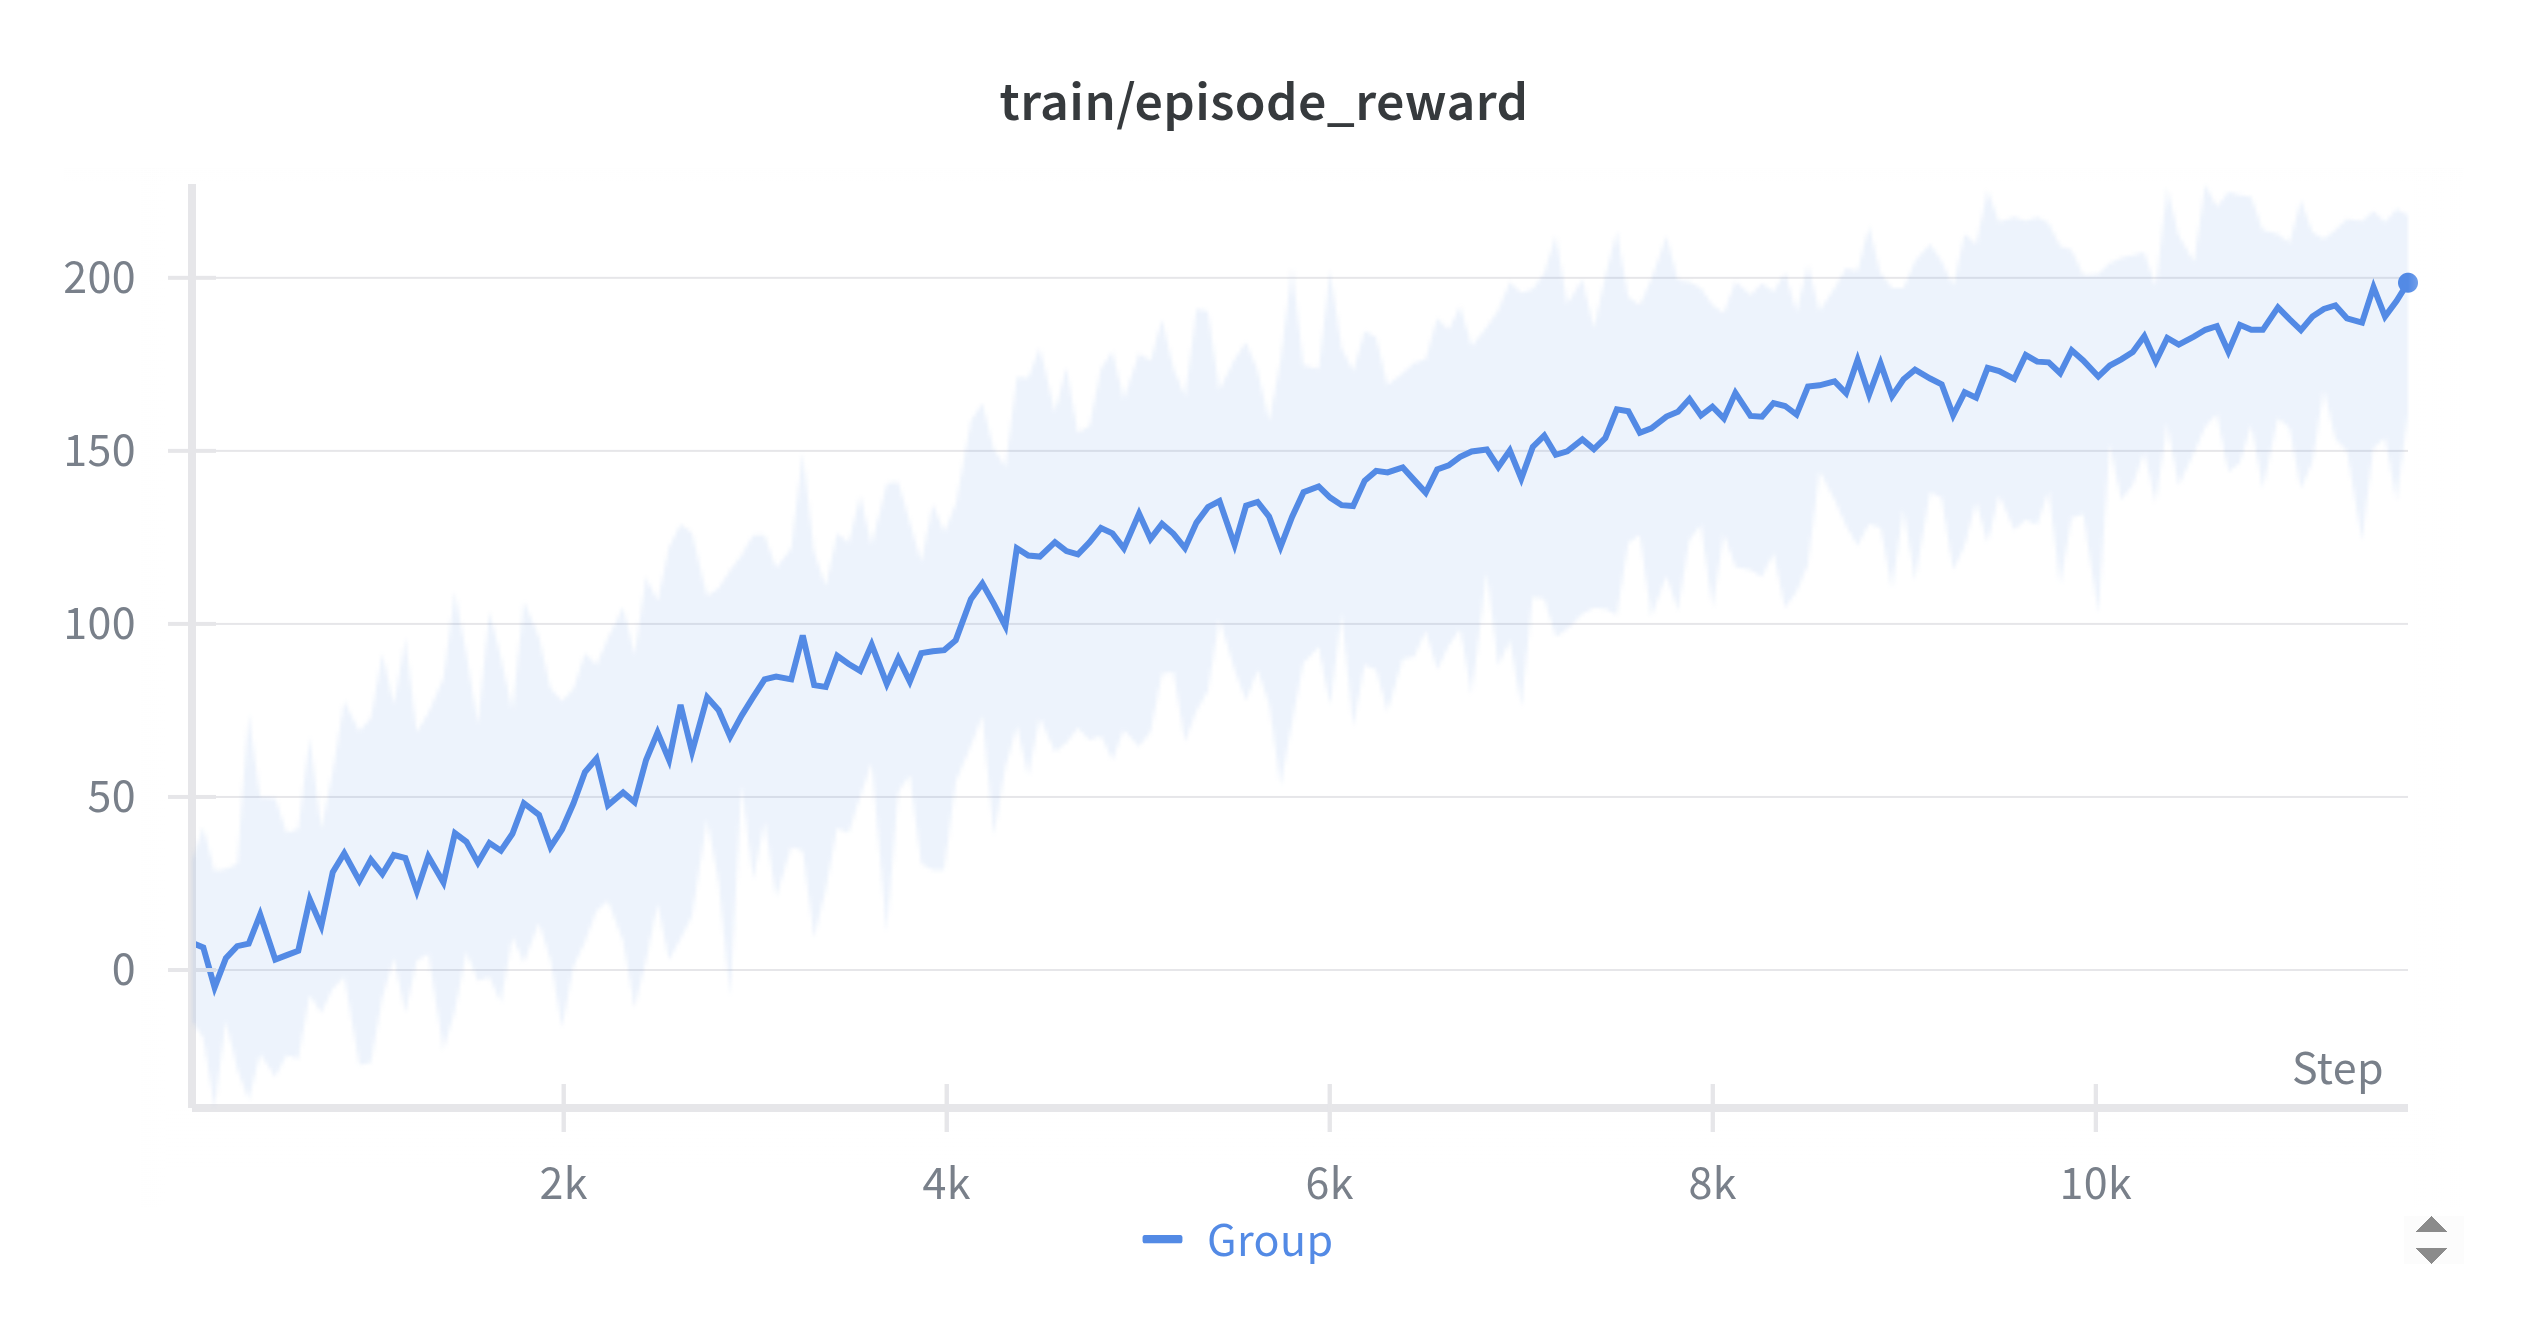
\includegraphics[width=0.7\linewidth]{photos/rew ppo - raw - 1 - norm.png}
\caption{پاداش دوره \lr{PPO} \lr{--} پاداش بازدهی خامِ نرمال‌شده \lr{--} محیط تک‌گانه \lr{--} دوره‌های عادی}
\label{fig:ppo-raw-1env-normal}
\end{figure}


\begin{figure}[H]
\centering
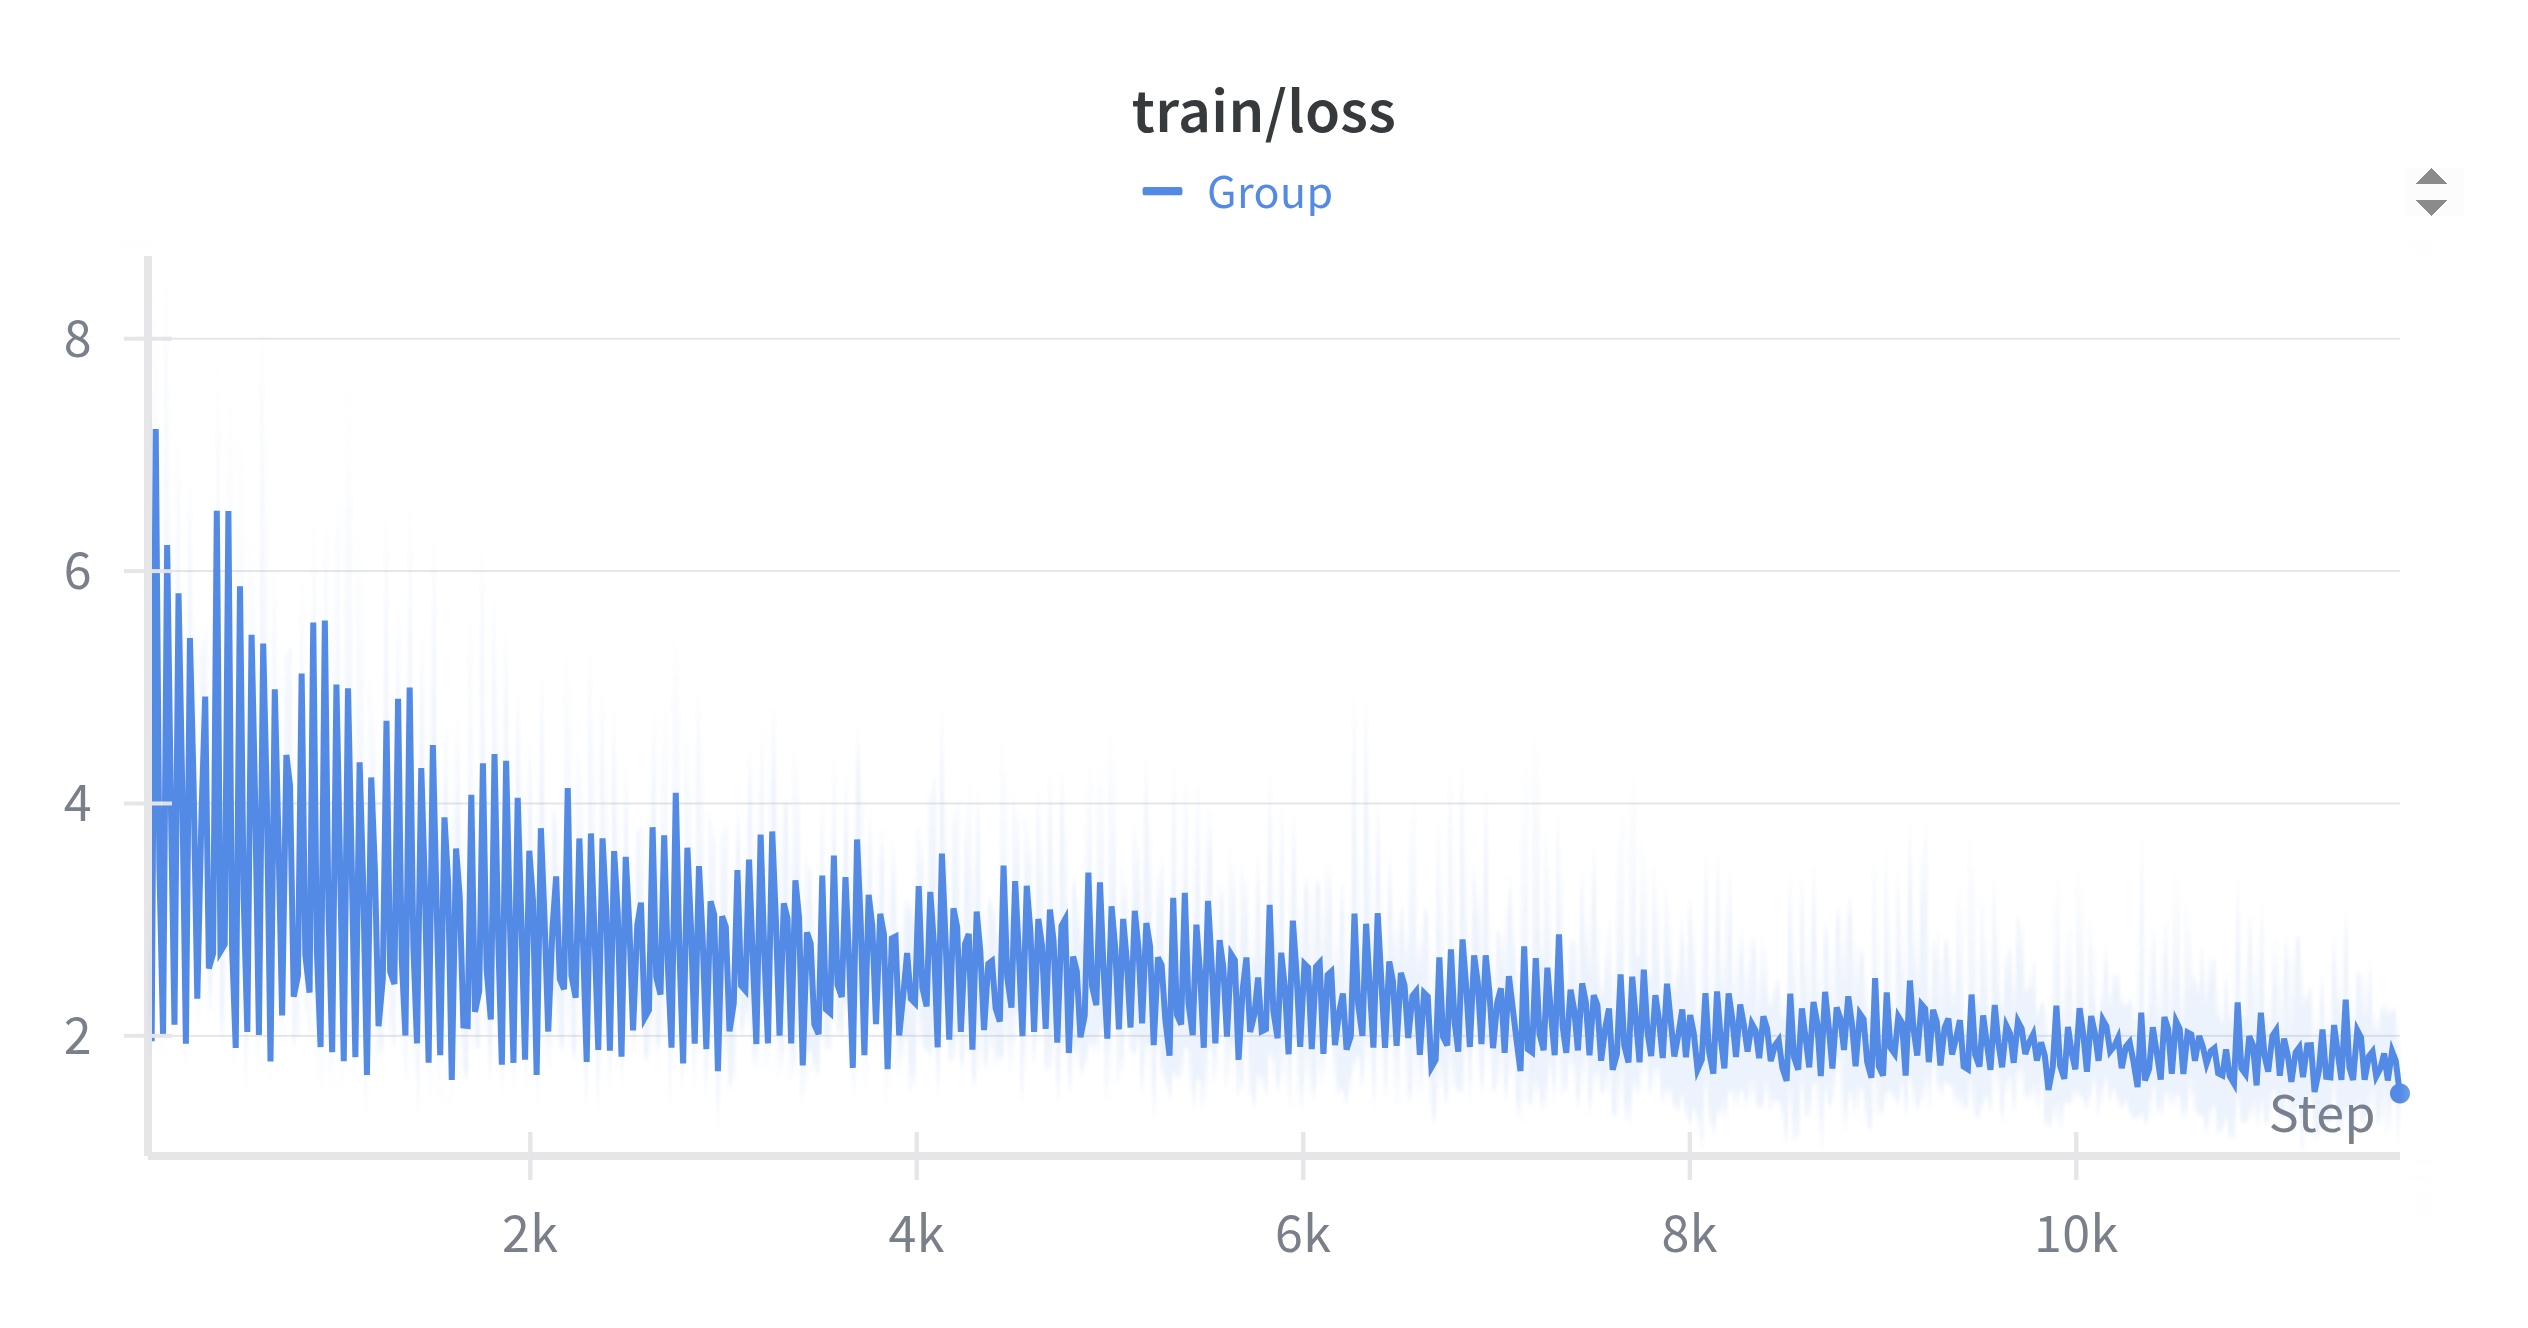
\includegraphics[width=0.7\linewidth]{photos/loss ppo - raw - 1 - norm.png}
\caption{هزینه آموزش \lr{PPO} \lr{--} پاداش بازدهی خامِ نرمال‌شده \lr{--} محیط تک‌گانه \lr{--} دوره‌های عادی}
\label{fig:ppo-raw-1env-normal}
\end{figure}


\begin{table}[H]
\centering
\caption{نتایج \lr{PPO} \lr{--} پاداش بازدهی خامِ نرمال‌شده \lr{--} محیط تک‌گانه \lr{--} دوره‌های تصادفی}
\label{tab:ppo-raw-1env-random}
\begin{tabular}{l c}
\toprule
\lr{Metric} & \lr{Mean $\pm$ Std} \\
\midrule
\lr{Annualized Return [\%]} & \lr{21.35 $\pm$ 4.97} \\
\lr{Annualized Volatility [\%]} & \lr{19.25 $\pm$ 2.13} \\
\lr{Max Drawdown [\%]} & \lr{-23.43 $\pm$ 1.94} \\
\lr{Average Drawdown [\%]} & \lr{-6.05 $\pm$ 1.58} \\
\lr{Sharpe Ratio} & \lr{1.11 $\pm$ 0.22} \\
\lr{Sortino Ratio} & \lr{1.48 $\pm$ 0.29} \\
\lr{Calmar Ratio} & \lr{0.91 $\pm$ 0.20} \\
\lr{Max Drawdown Duration (days)} & \lr{182.70 $\pm$ 88.75} \\
\lr{Number of Trades} & \lr{124.70 $\pm$ 47.89} \\
\bottomrule
\end{tabular}
\end{table}


\begin{figure}[H]
\centering
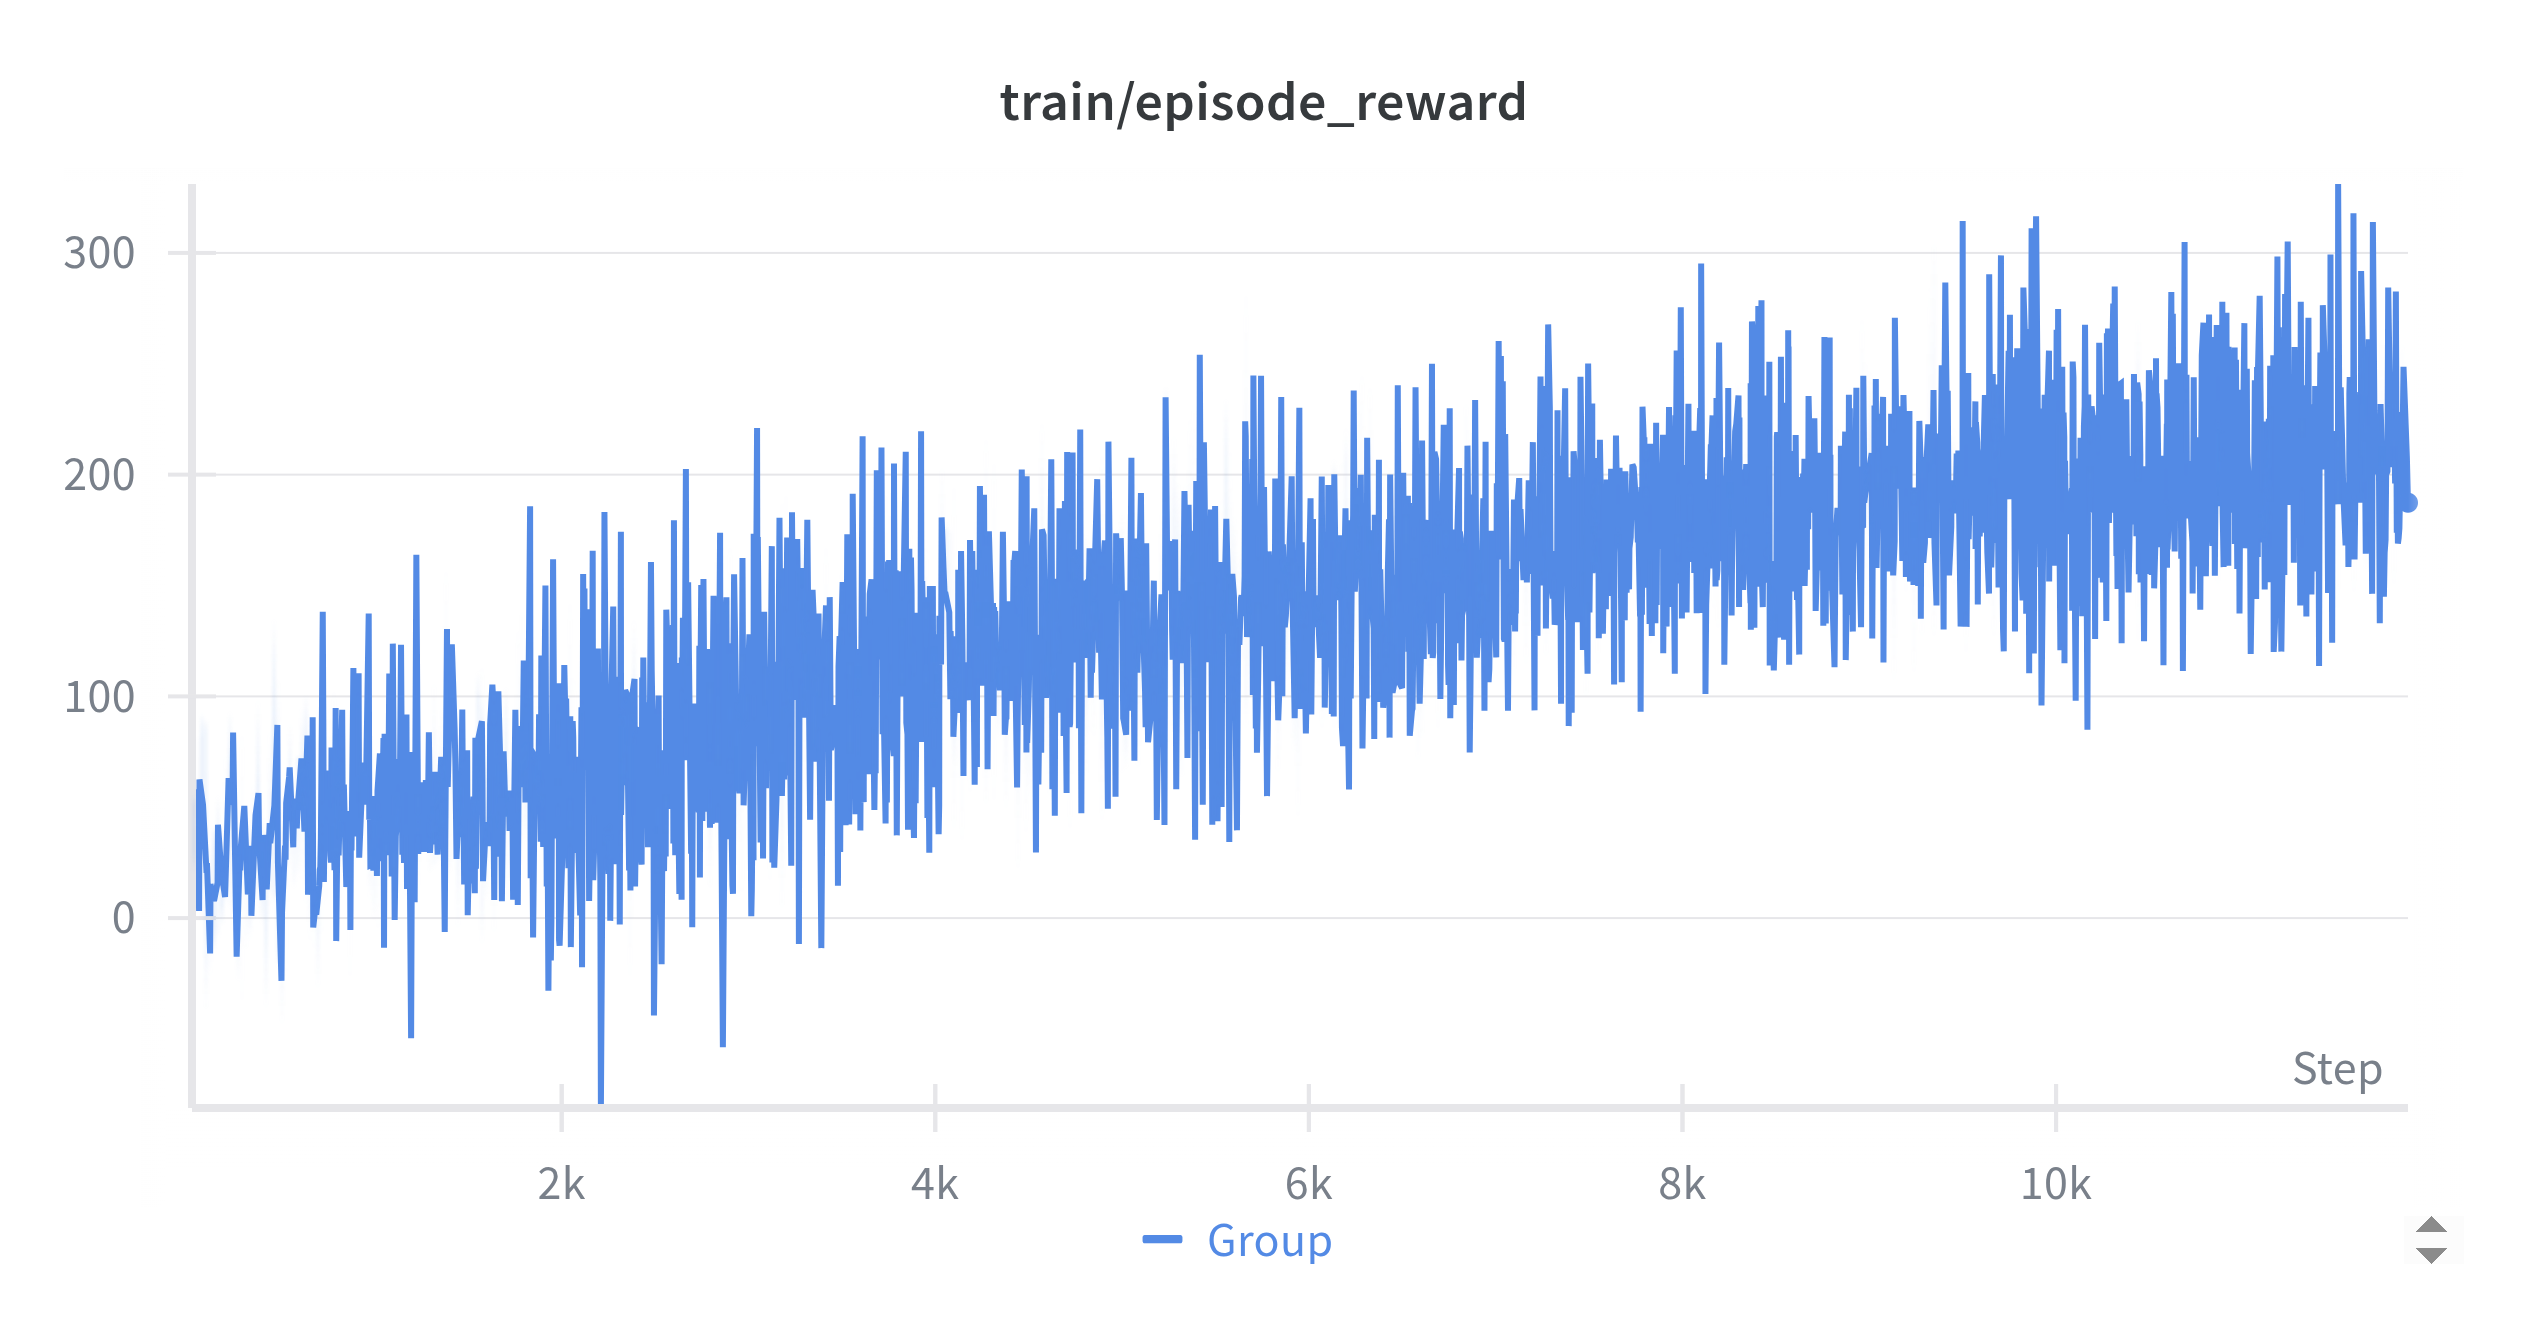
\includegraphics[width=0.7\linewidth]{photos/rew ppo - raw - 1 - rand.png} % مسیر عکس خودتان
\caption{پاداش دوره \lr{PPO} \lr{--} پاداش بازدهی خامِ نرمال‌شده \lr{--} محیط تک‌گانه \lr{--} دوره‌های تصادفی}
\label{fig:ppo-raw-1env-random}
\end{figure}


\begin{figure}[H]
\centering
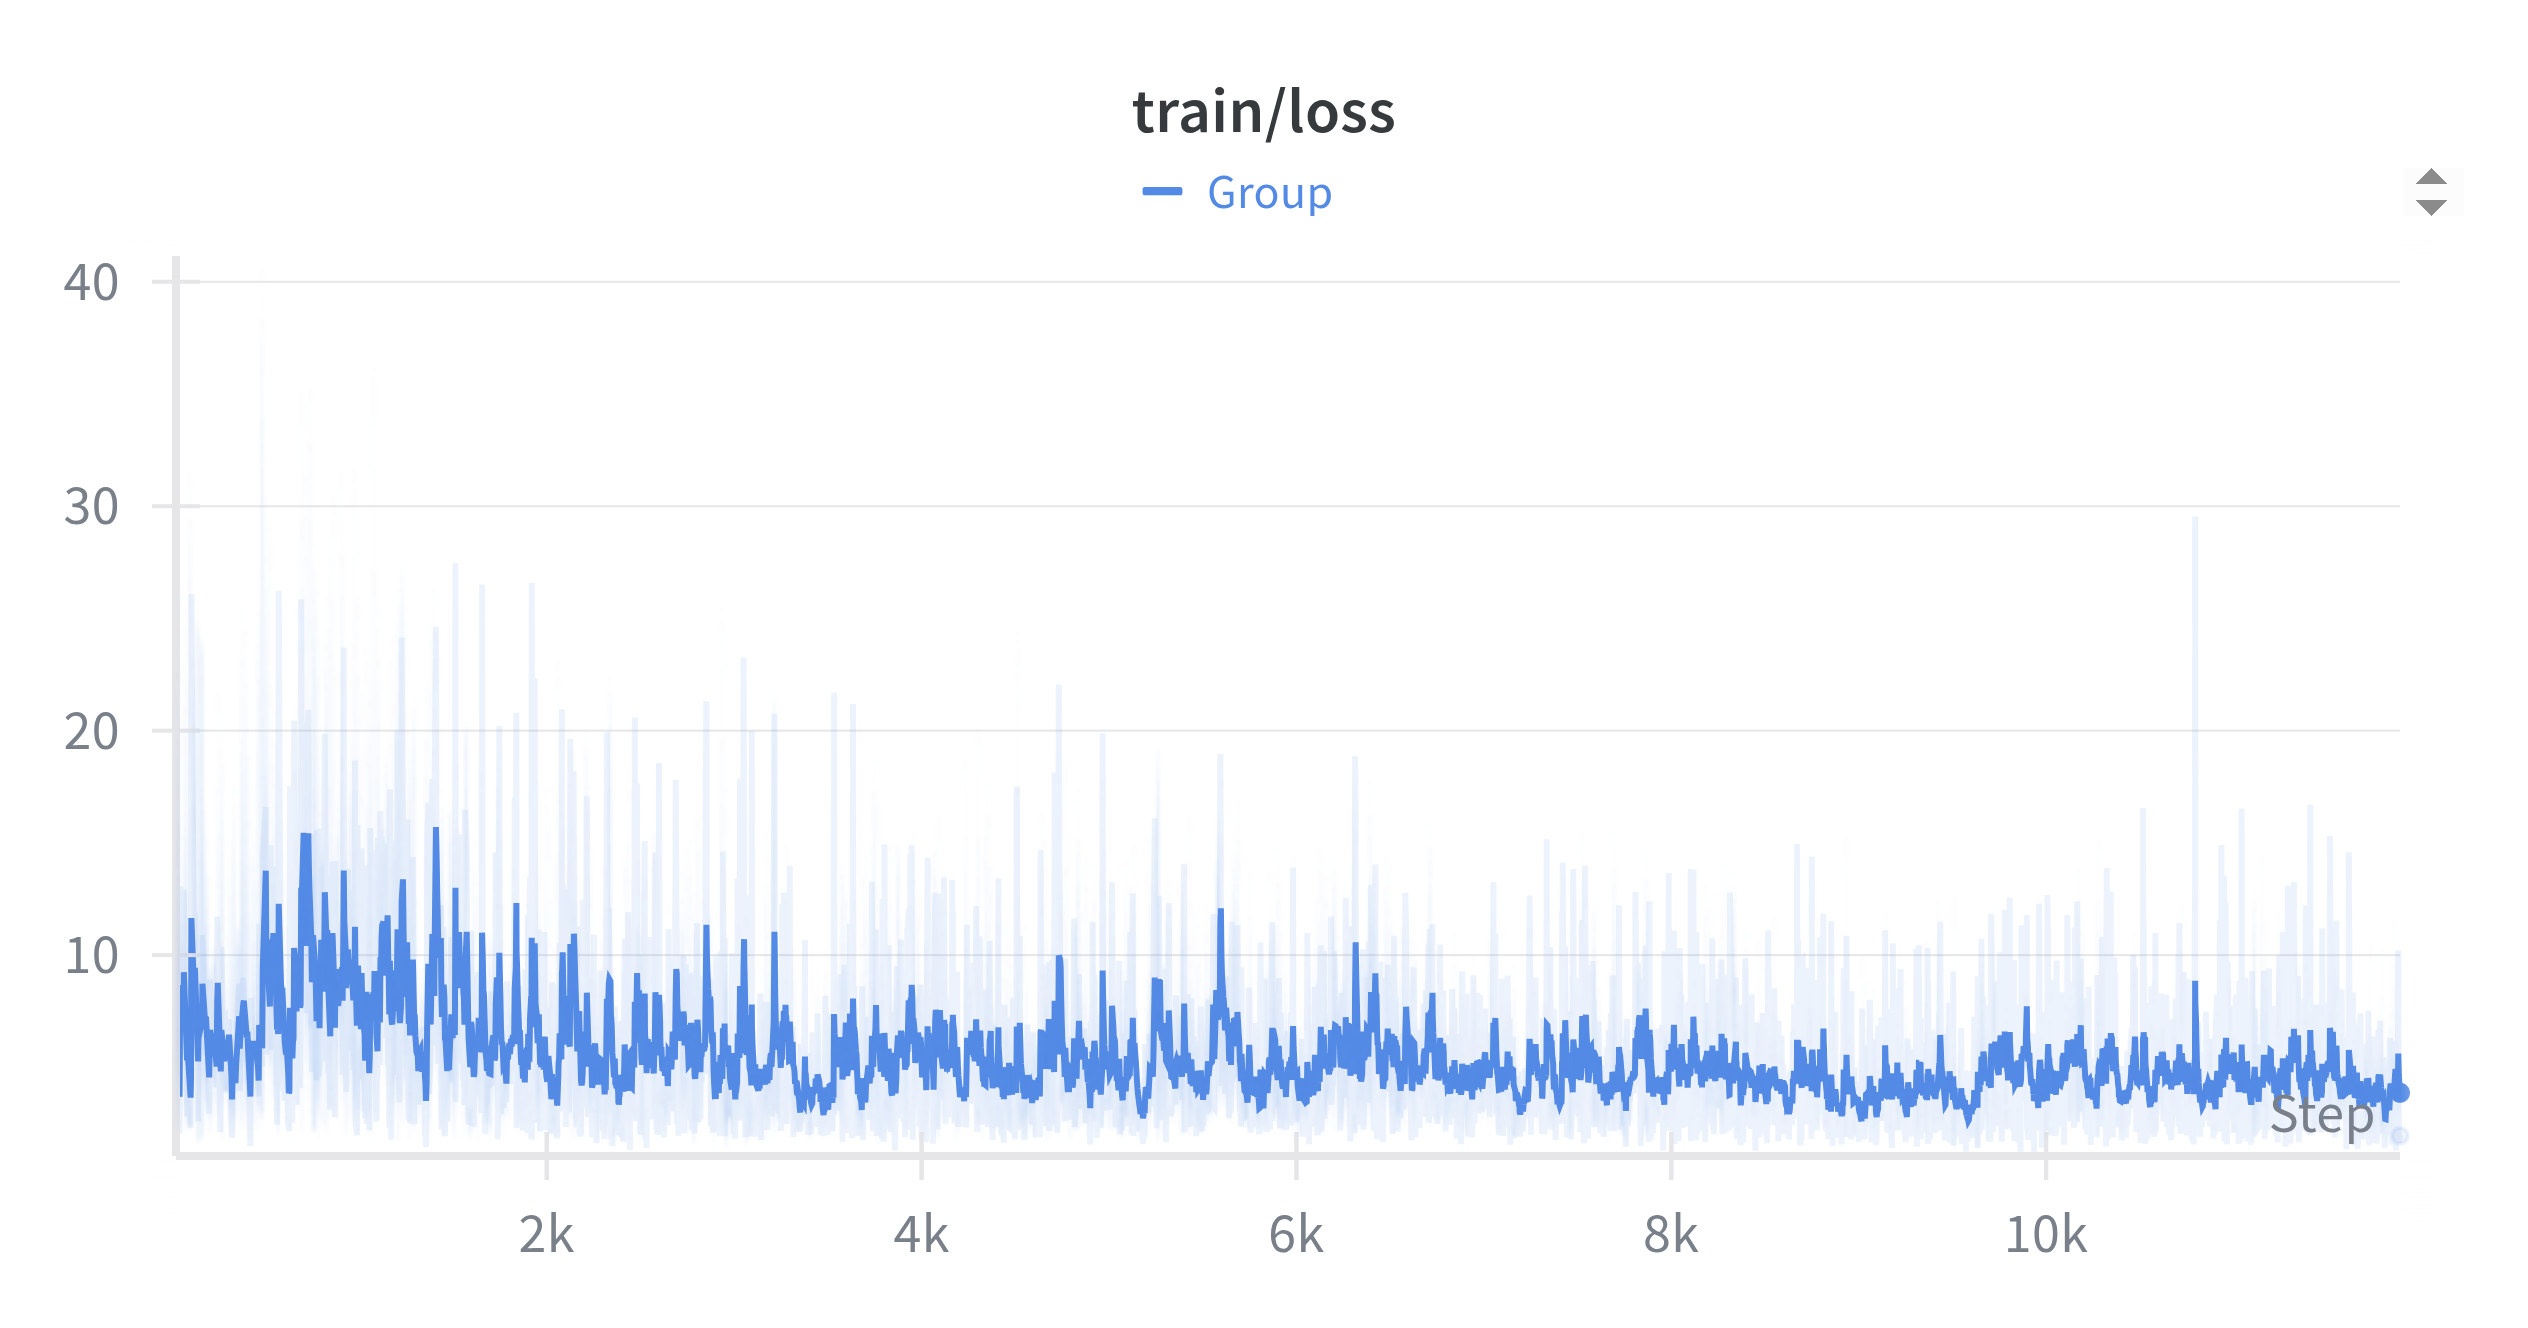
\includegraphics[width=0.7\linewidth]{photos/loss ppo - raw - 1 - rand.png} % مسیر عکس خودتان
\caption{هزینه آموزش \lr{PPO} \lr{--} پاداش بازدهی خامِ نرمال‌شده \lr{--} محیط تک‌گانه \lr{--} دوره‌های تصادفی}
\label{fig:ppo-raw-1env-random}
\end{figure}


\begin{table}[H]
\centering
\caption{نتایج \lr{PPO} \lr{--} پاداش بازدهی خامِ نرمال‌شده \lr{--} محیط‌های برداری (۳-محیط) \lr{--} دوره‌های عادی}
\label{tab:ppo-raw-3env-normal}
\begin{tabular}{l c}
\toprule
\lr{Metric} & \lr{Mean $\pm$ Std} \\
\midrule
\lr{Annualized Return [\%]} & \lr{19.10 $\pm$ 3.98} \\
\lr{Annualized Volatility [\%]} & \lr{21.25 $\pm$ 1.35} \\
\lr{Max Drawdown [\%]} & \lr{-24.33 $\pm$ 2.20} \\
\lr{Average Drawdown [\%]} & \lr{-7.79 $\pm$ 1.21} \\
\lr{Sharpe Ratio} & \lr{0.93 $\pm$ 0.14} \\
\lr{Sortino Ratio} & \lr{1.24 $\pm$ 0.18} \\
\lr{Calmar Ratio} & \lr{0.79 $\pm$ 0.18} \\
\lr{Max Drawdown Duration (days)} & \lr{250.20 $\pm$ 108.01} \\
\lr{Number of Trades} & \lr{139.60 $\pm$ 11.89} \\
\bottomrule
\end{tabular}
\end{table}

\begin{figure}[H]
\centering
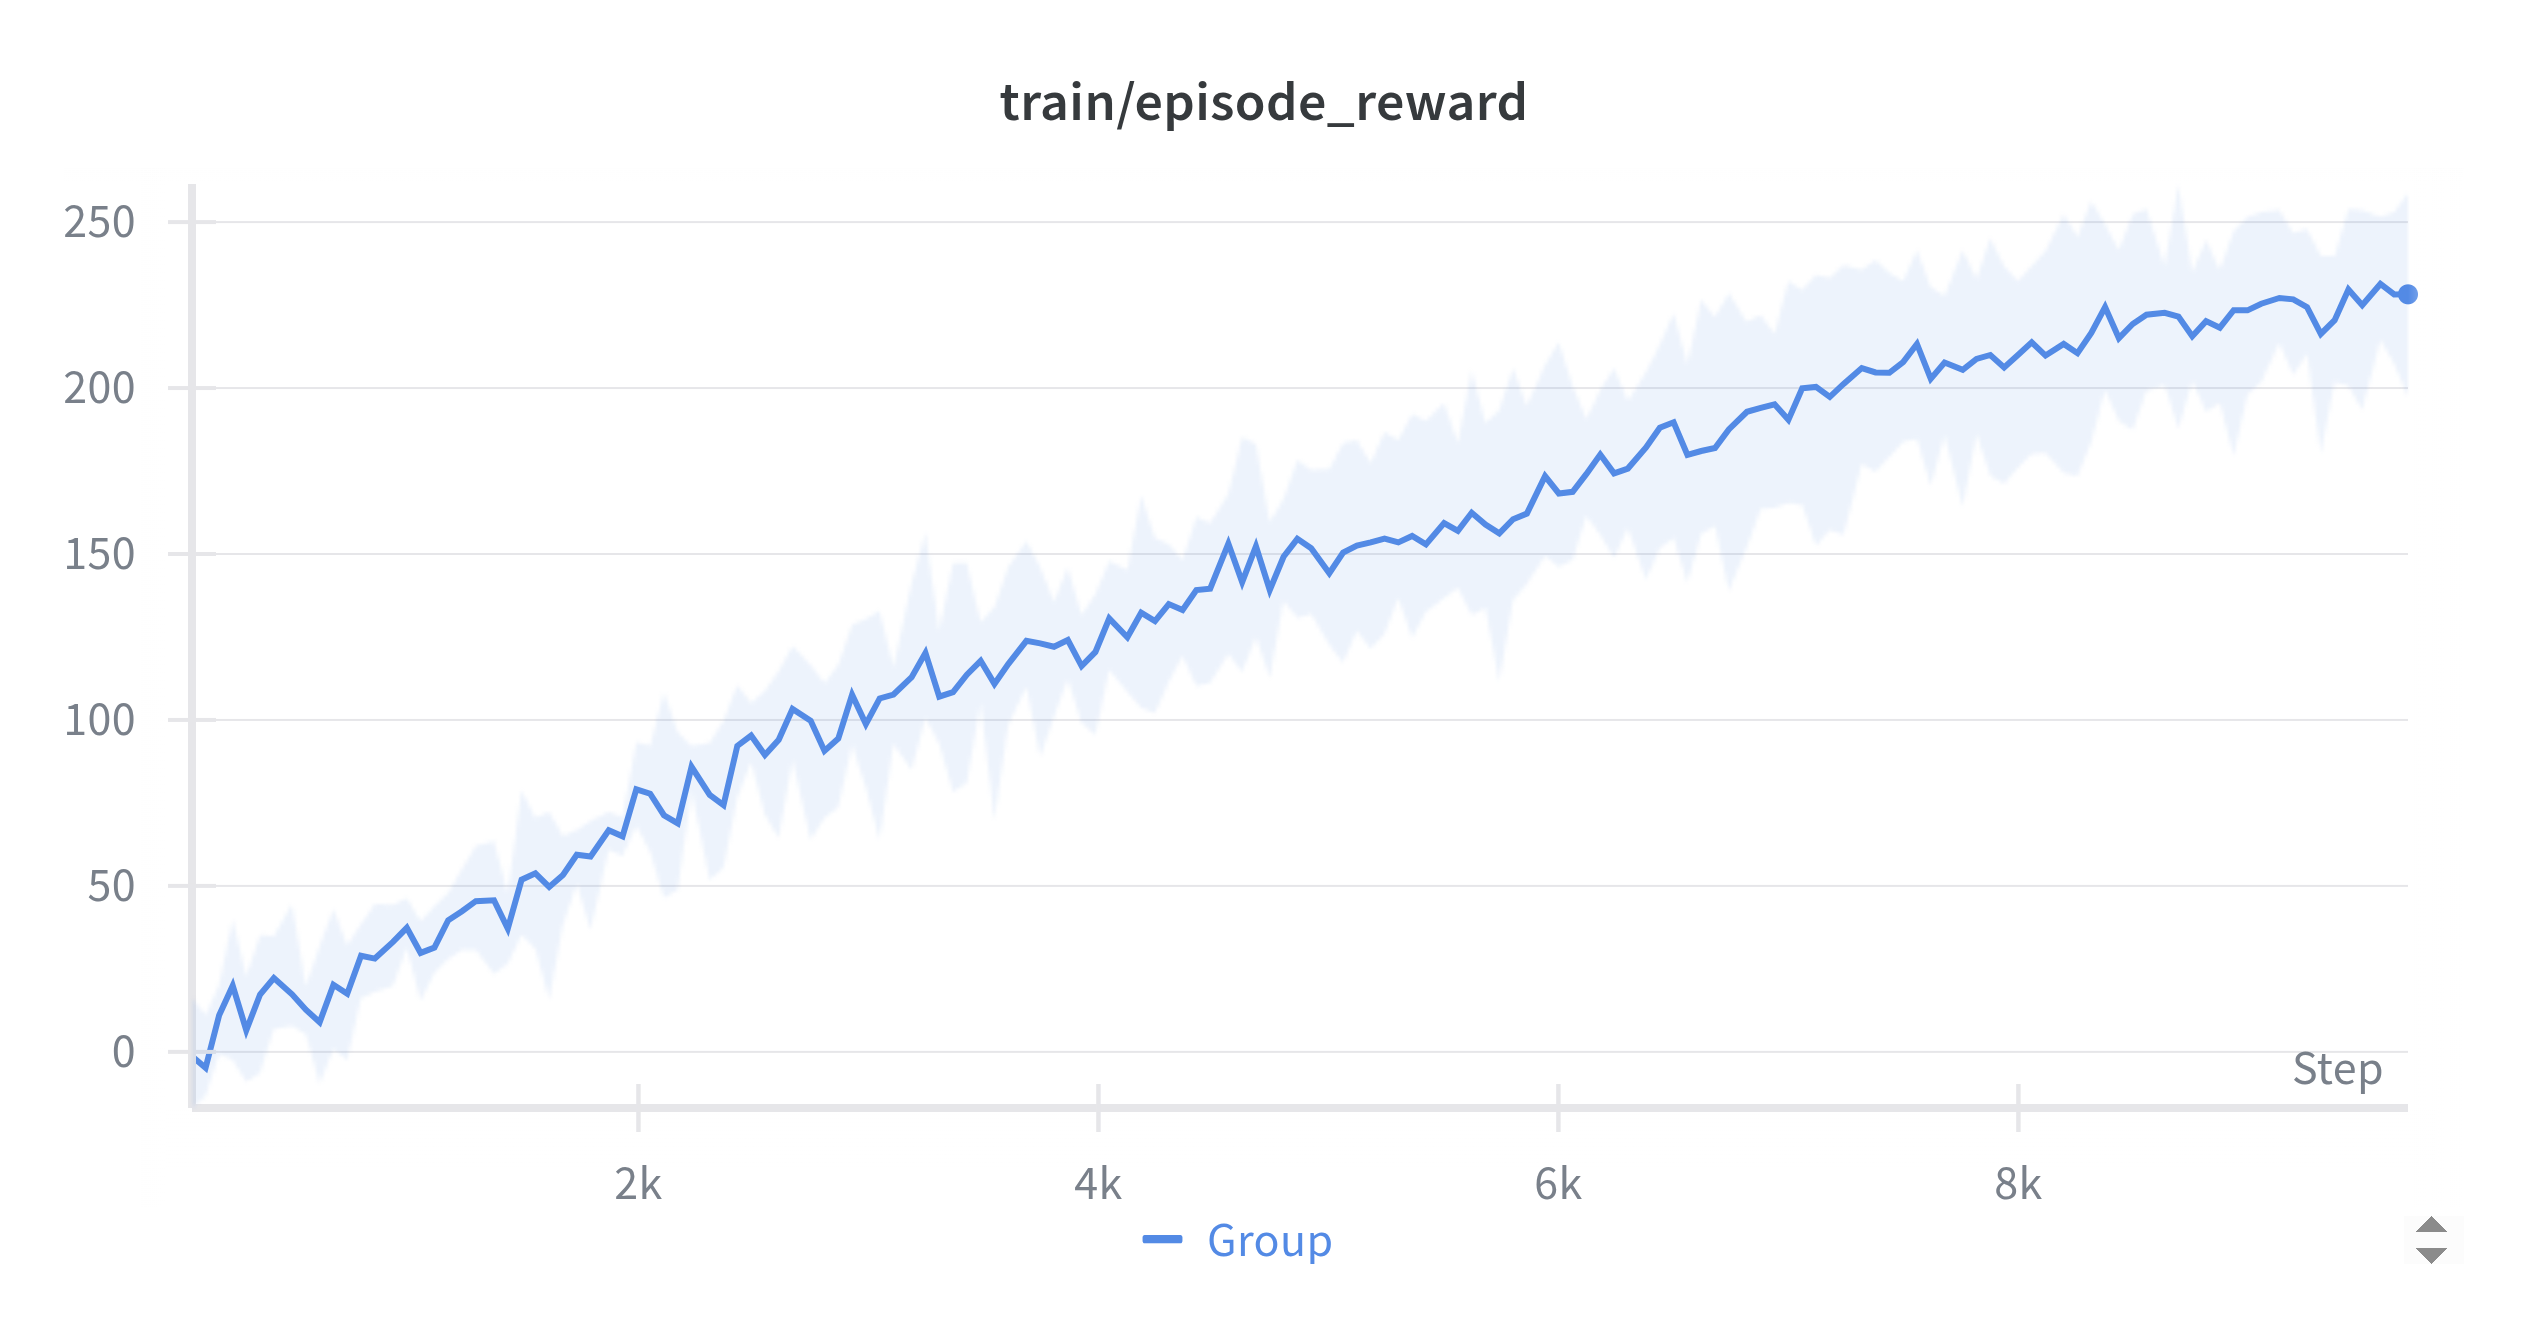
\includegraphics[width=0.7\linewidth]{photos/rew ppo - raw - 3 - norm.png} % مسیر فایل عکس را جایگزین کنید
\caption{پاداش دوره \lr{PPO} \lr{--} پاداش بازدهی خامِ نرمال‌شده \lr{--} محیط‌های برداری (۳-محیط) \lr{--} دوره‌های عادی}
\label{tab:ppo-raw-3env-normal}
\end{figure}



\begin{figure}[H]
\centering
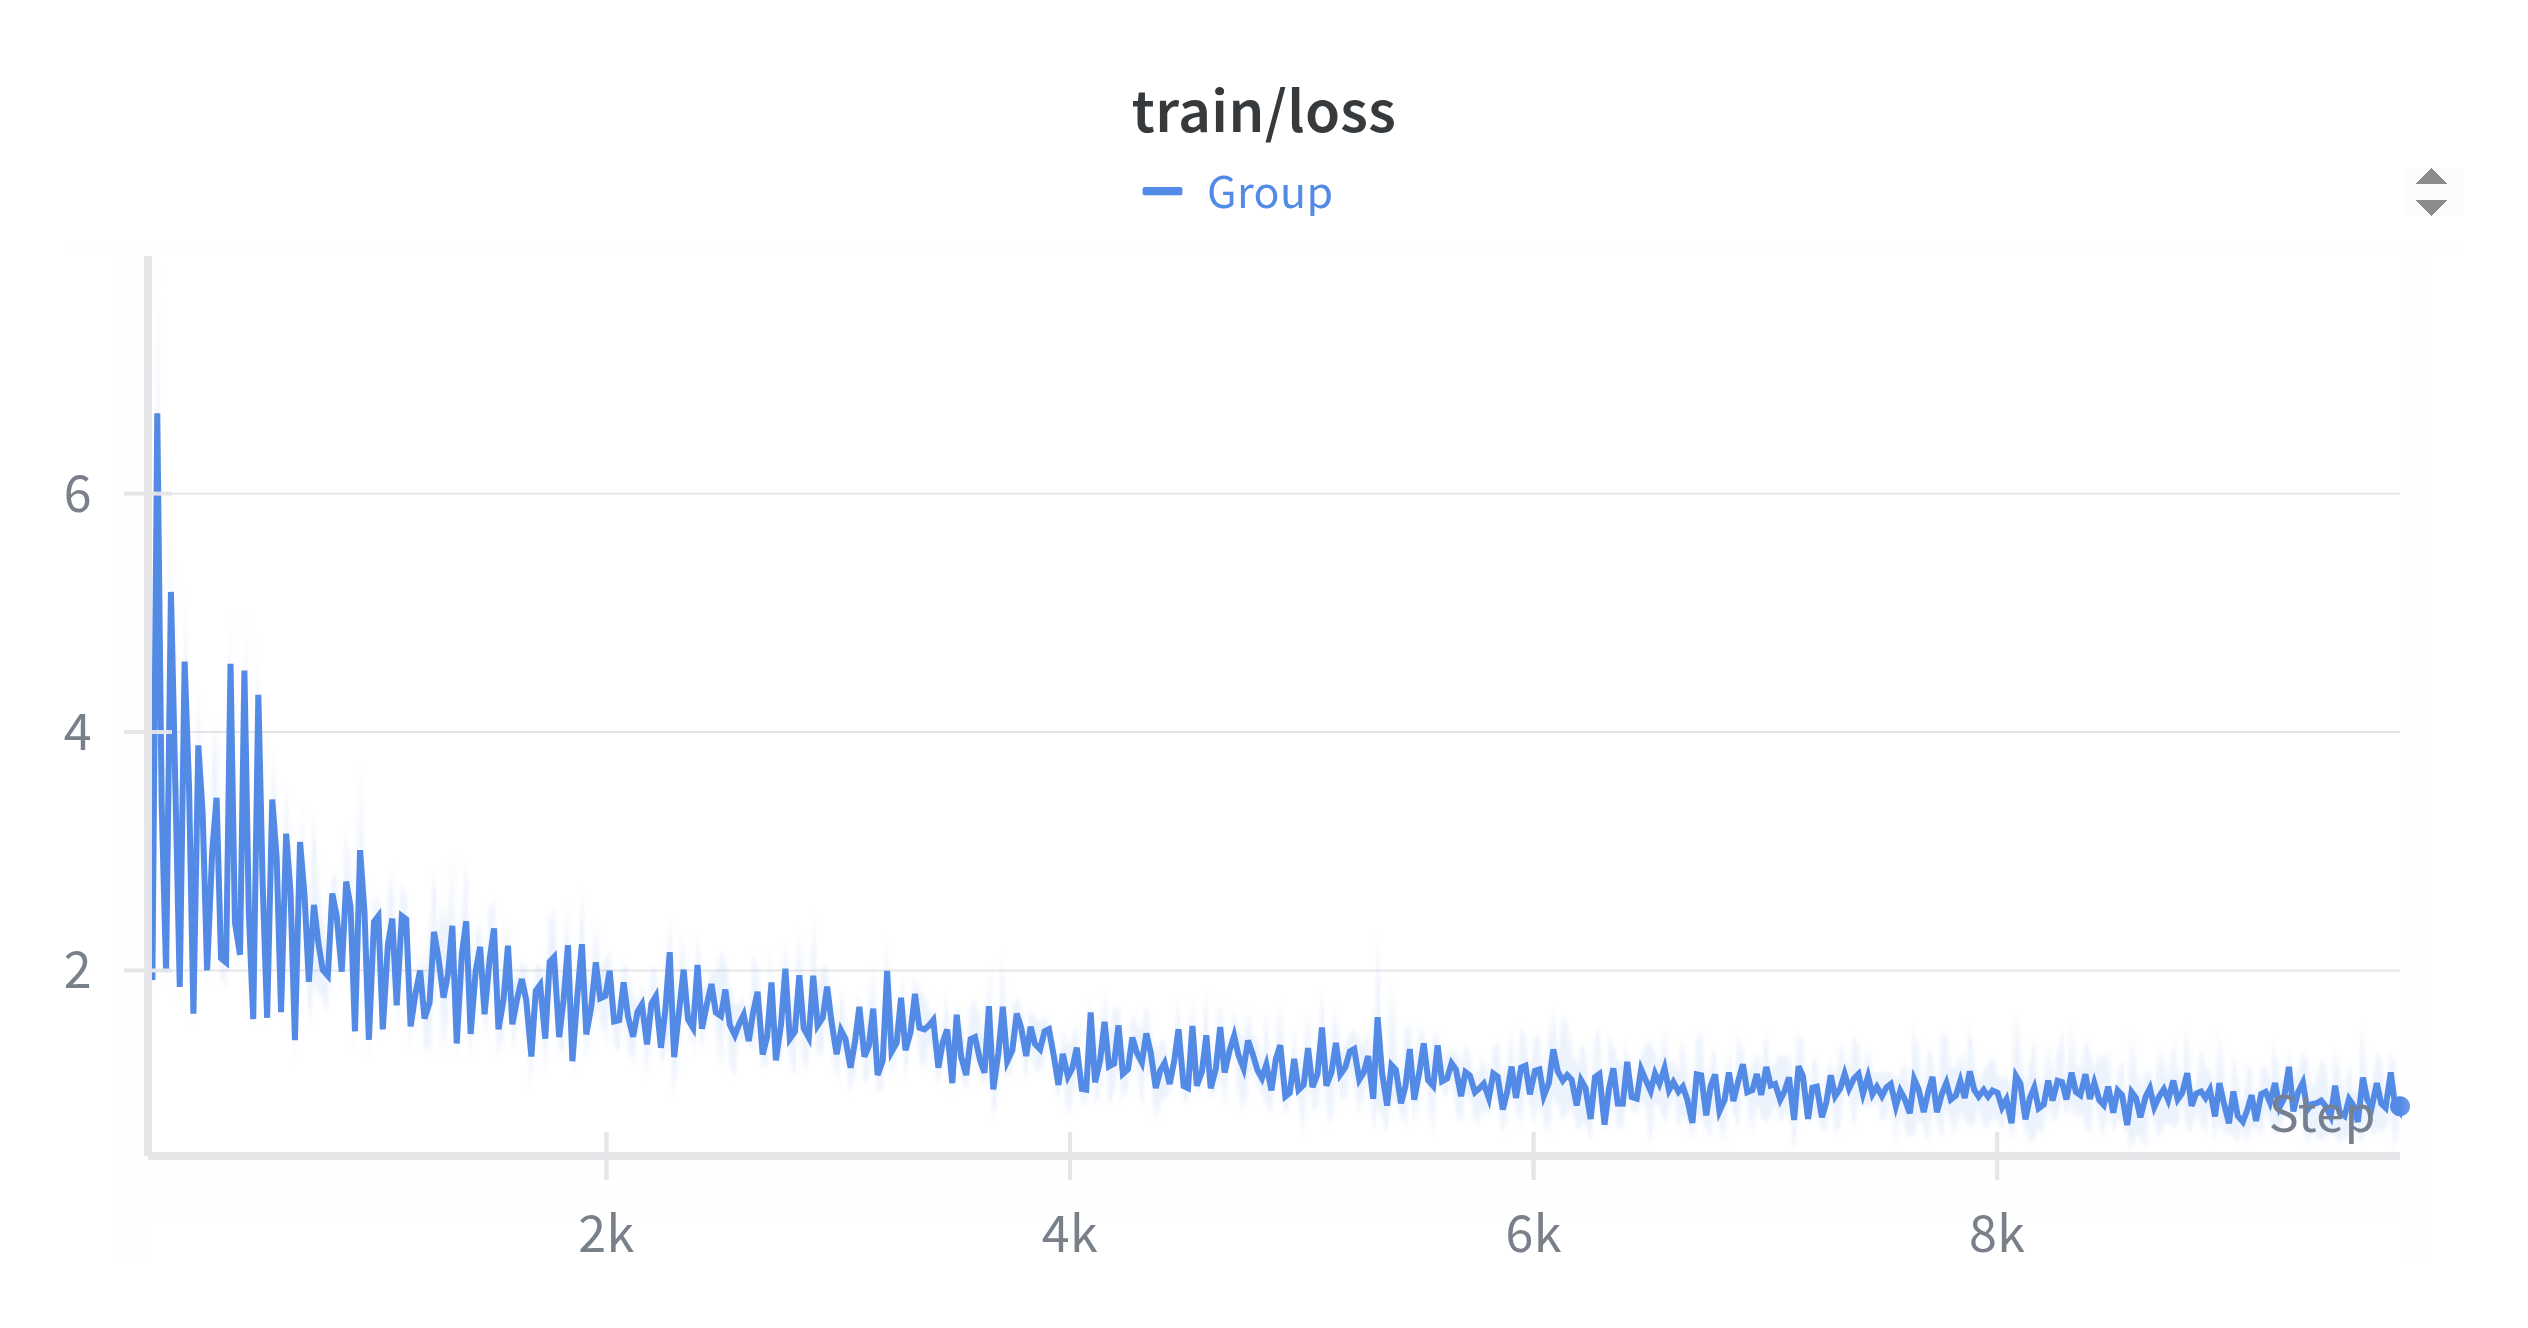
\includegraphics[width=0.7\linewidth]{photos/loss ppo - raw - 3 - norm.png} % مسیر فایل عکس را جایگزین کنید
\caption{پاداش دوره \lr{PPO} \lr{--} پاداش بازدهی خامِ نرمال‌شده \lr{--} محیط‌های برداری (۳-محیط) \lr{--} دوره‌های عادی}
\label{tab:ppo-raw-3env-normal}
\end{figure}



\begin{table}[H]
\centering
\caption{نتایج \lr{PPO} \lr{--} پاداشبازدهی خامِ نرمال‌شده \lr{--} محیط‌های برداری (۳-محیط) \lr{--} دوره‌های تصادفی}
\label{tab:ppo-raw-3env-random}
\begin{tabular}{l c}
\toprule
\lr{Metric} & \lr{Mean $\pm$ Std} \\
\midrule
\lr{Annualized Return [\%]} & \lr{20.89 $\pm$ 4.75} \\
\lr{Annualized Volatility [\%]} & \lr{19.21 $\pm$ 2.86} \\
\lr{Max Drawdown [\%]} & \lr{-23.24 $\pm$ 2.86} \\
\lr{Average Drawdown [\%]} & \lr{-5.62 $\pm$ 1.48} \\
\lr{Sharpe Ratio} & \lr{1.09 $\pm$ 0.16} \\
\lr{Sortino Ratio} & \lr{1.45 $\pm$ 0.20} \\
\lr{Calmar Ratio} & \lr{0.90 $\pm$ 0.15} \\
\lr{Max Drawdown Duration (days)} & \lr{154.25 $\pm$ 69.62} \\
\lr{Number of Trades} & \lr{154.00 $\pm$ 33.93} \\
\bottomrule
\end{tabular}
\end{table}


\begin{figure}[H]
\centering
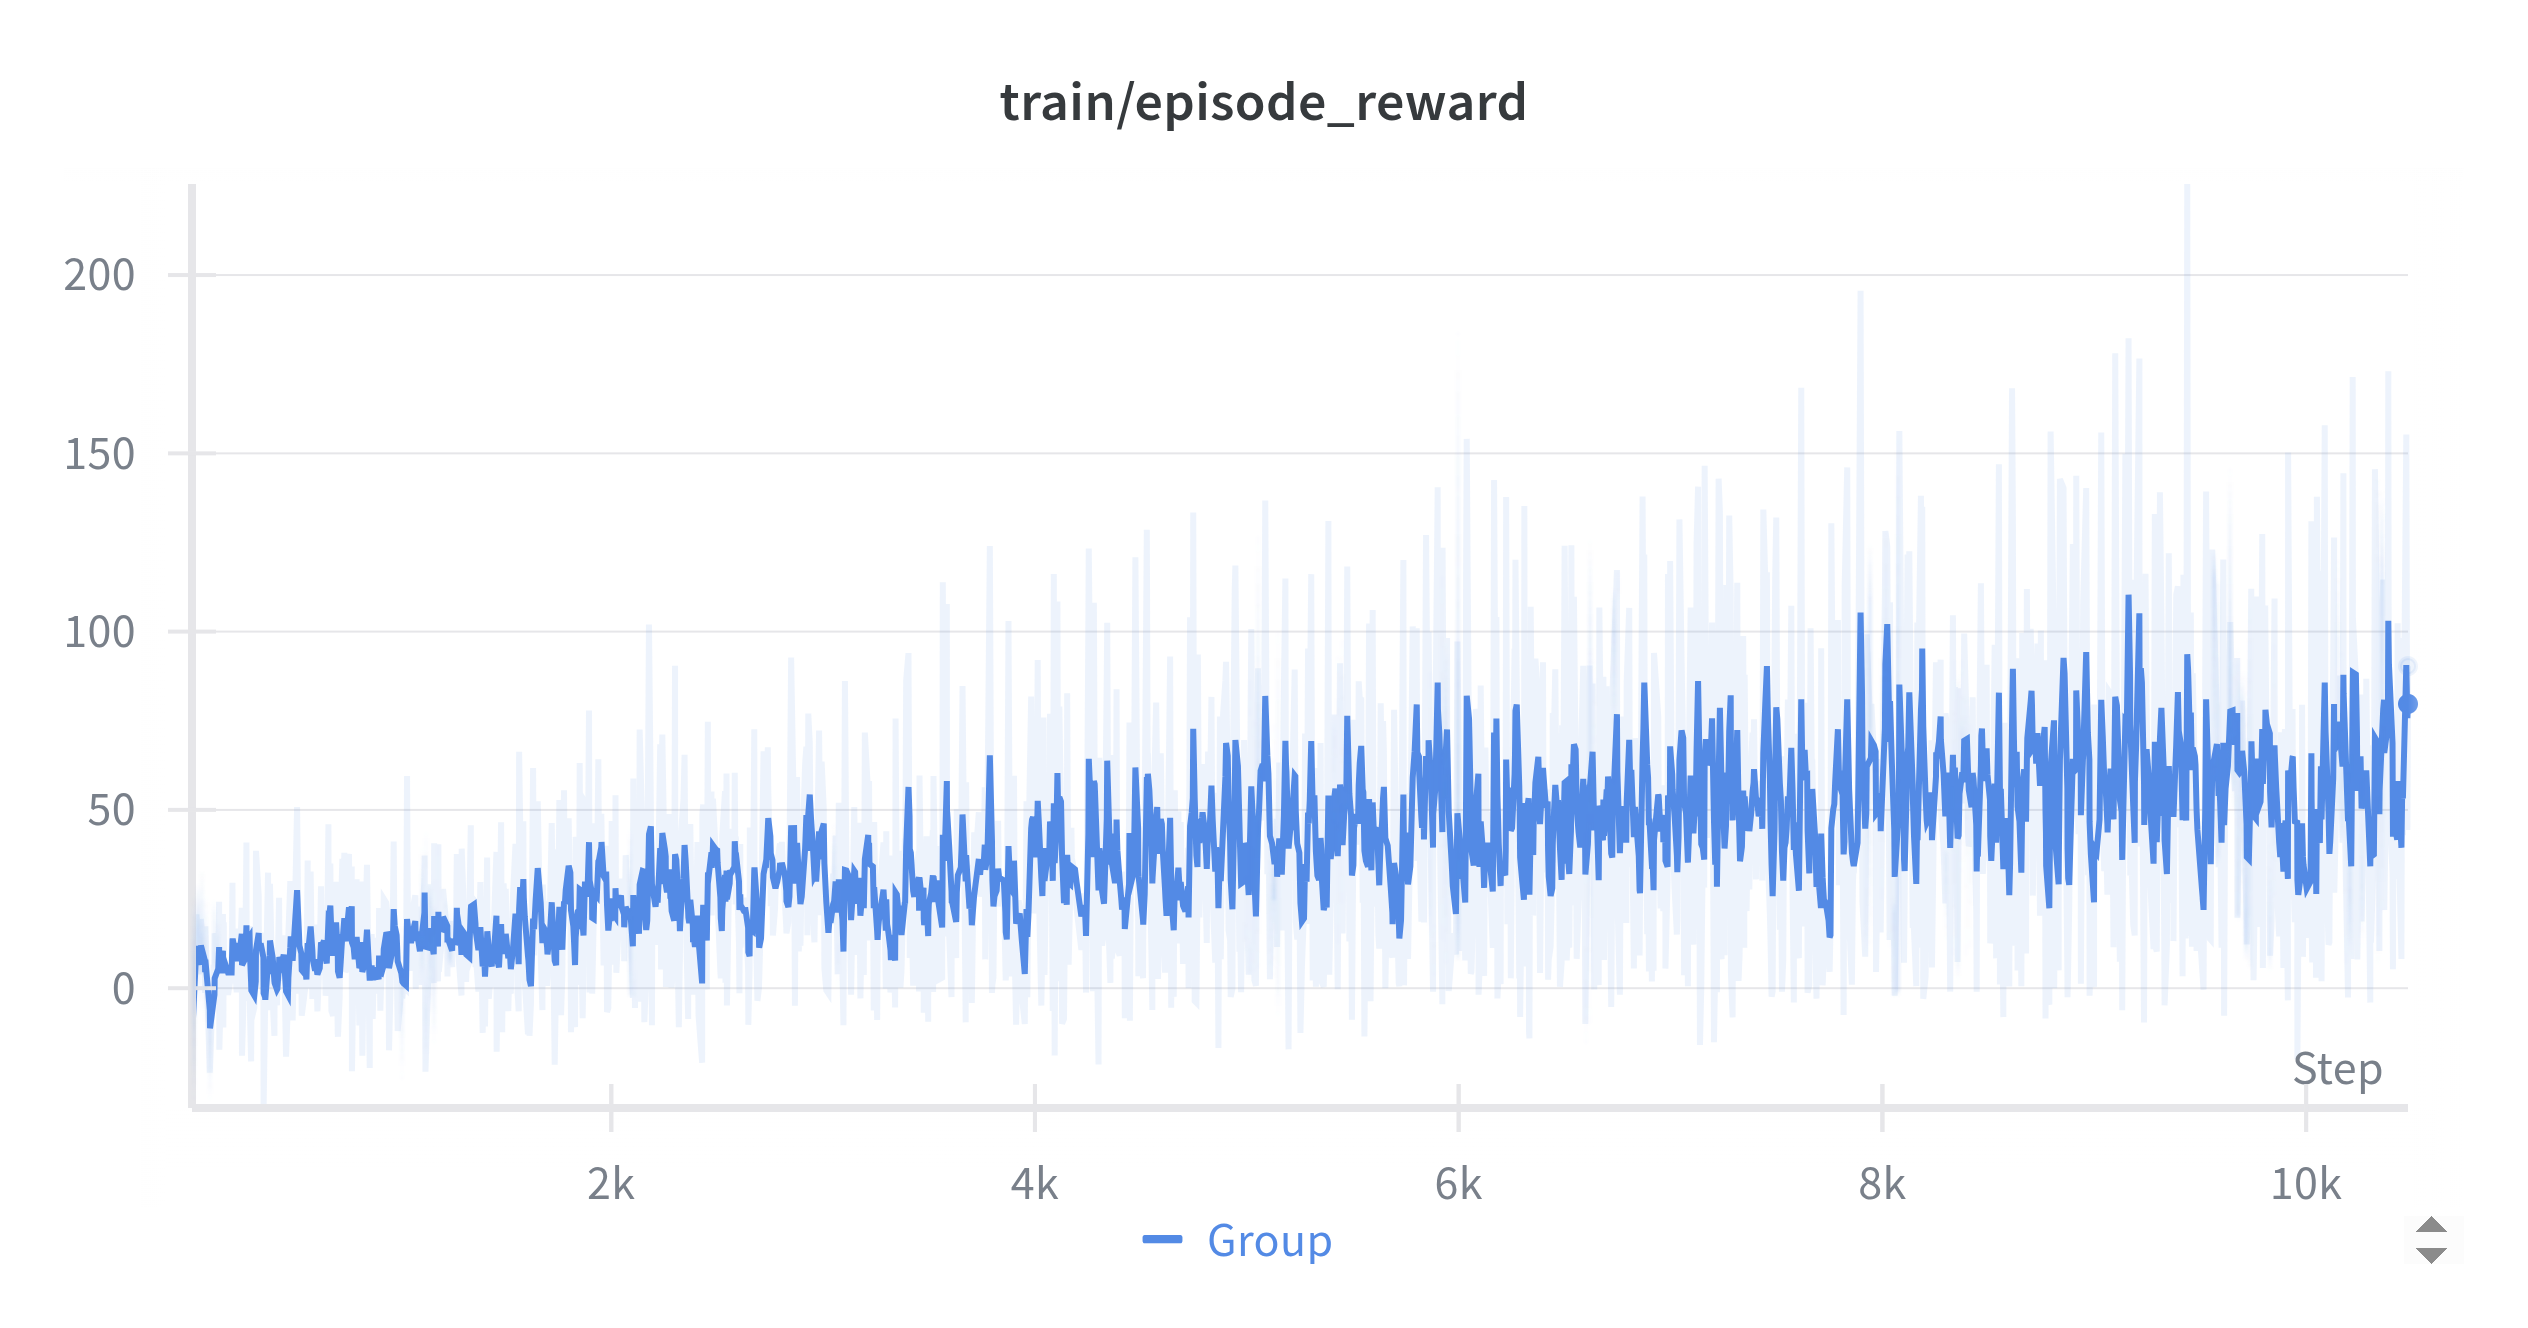
\includegraphics[width=0.7\linewidth]{photos/rew ppo - raw - 3 - rand.png} % مسیر فایل عکس را جایگزین کنید
\caption{پاداش دوره \lr{PPO} \lr{--} پاداش بازدهی خامِ نرمال‌شده \lr{--} محیط‌های برداری (۳-محیط) \lr{--} دوره‌های تصادفی}
\label{tab:ppo-raw-3env-normal}
\end{figure}



\begin{figure}[H]
\centering
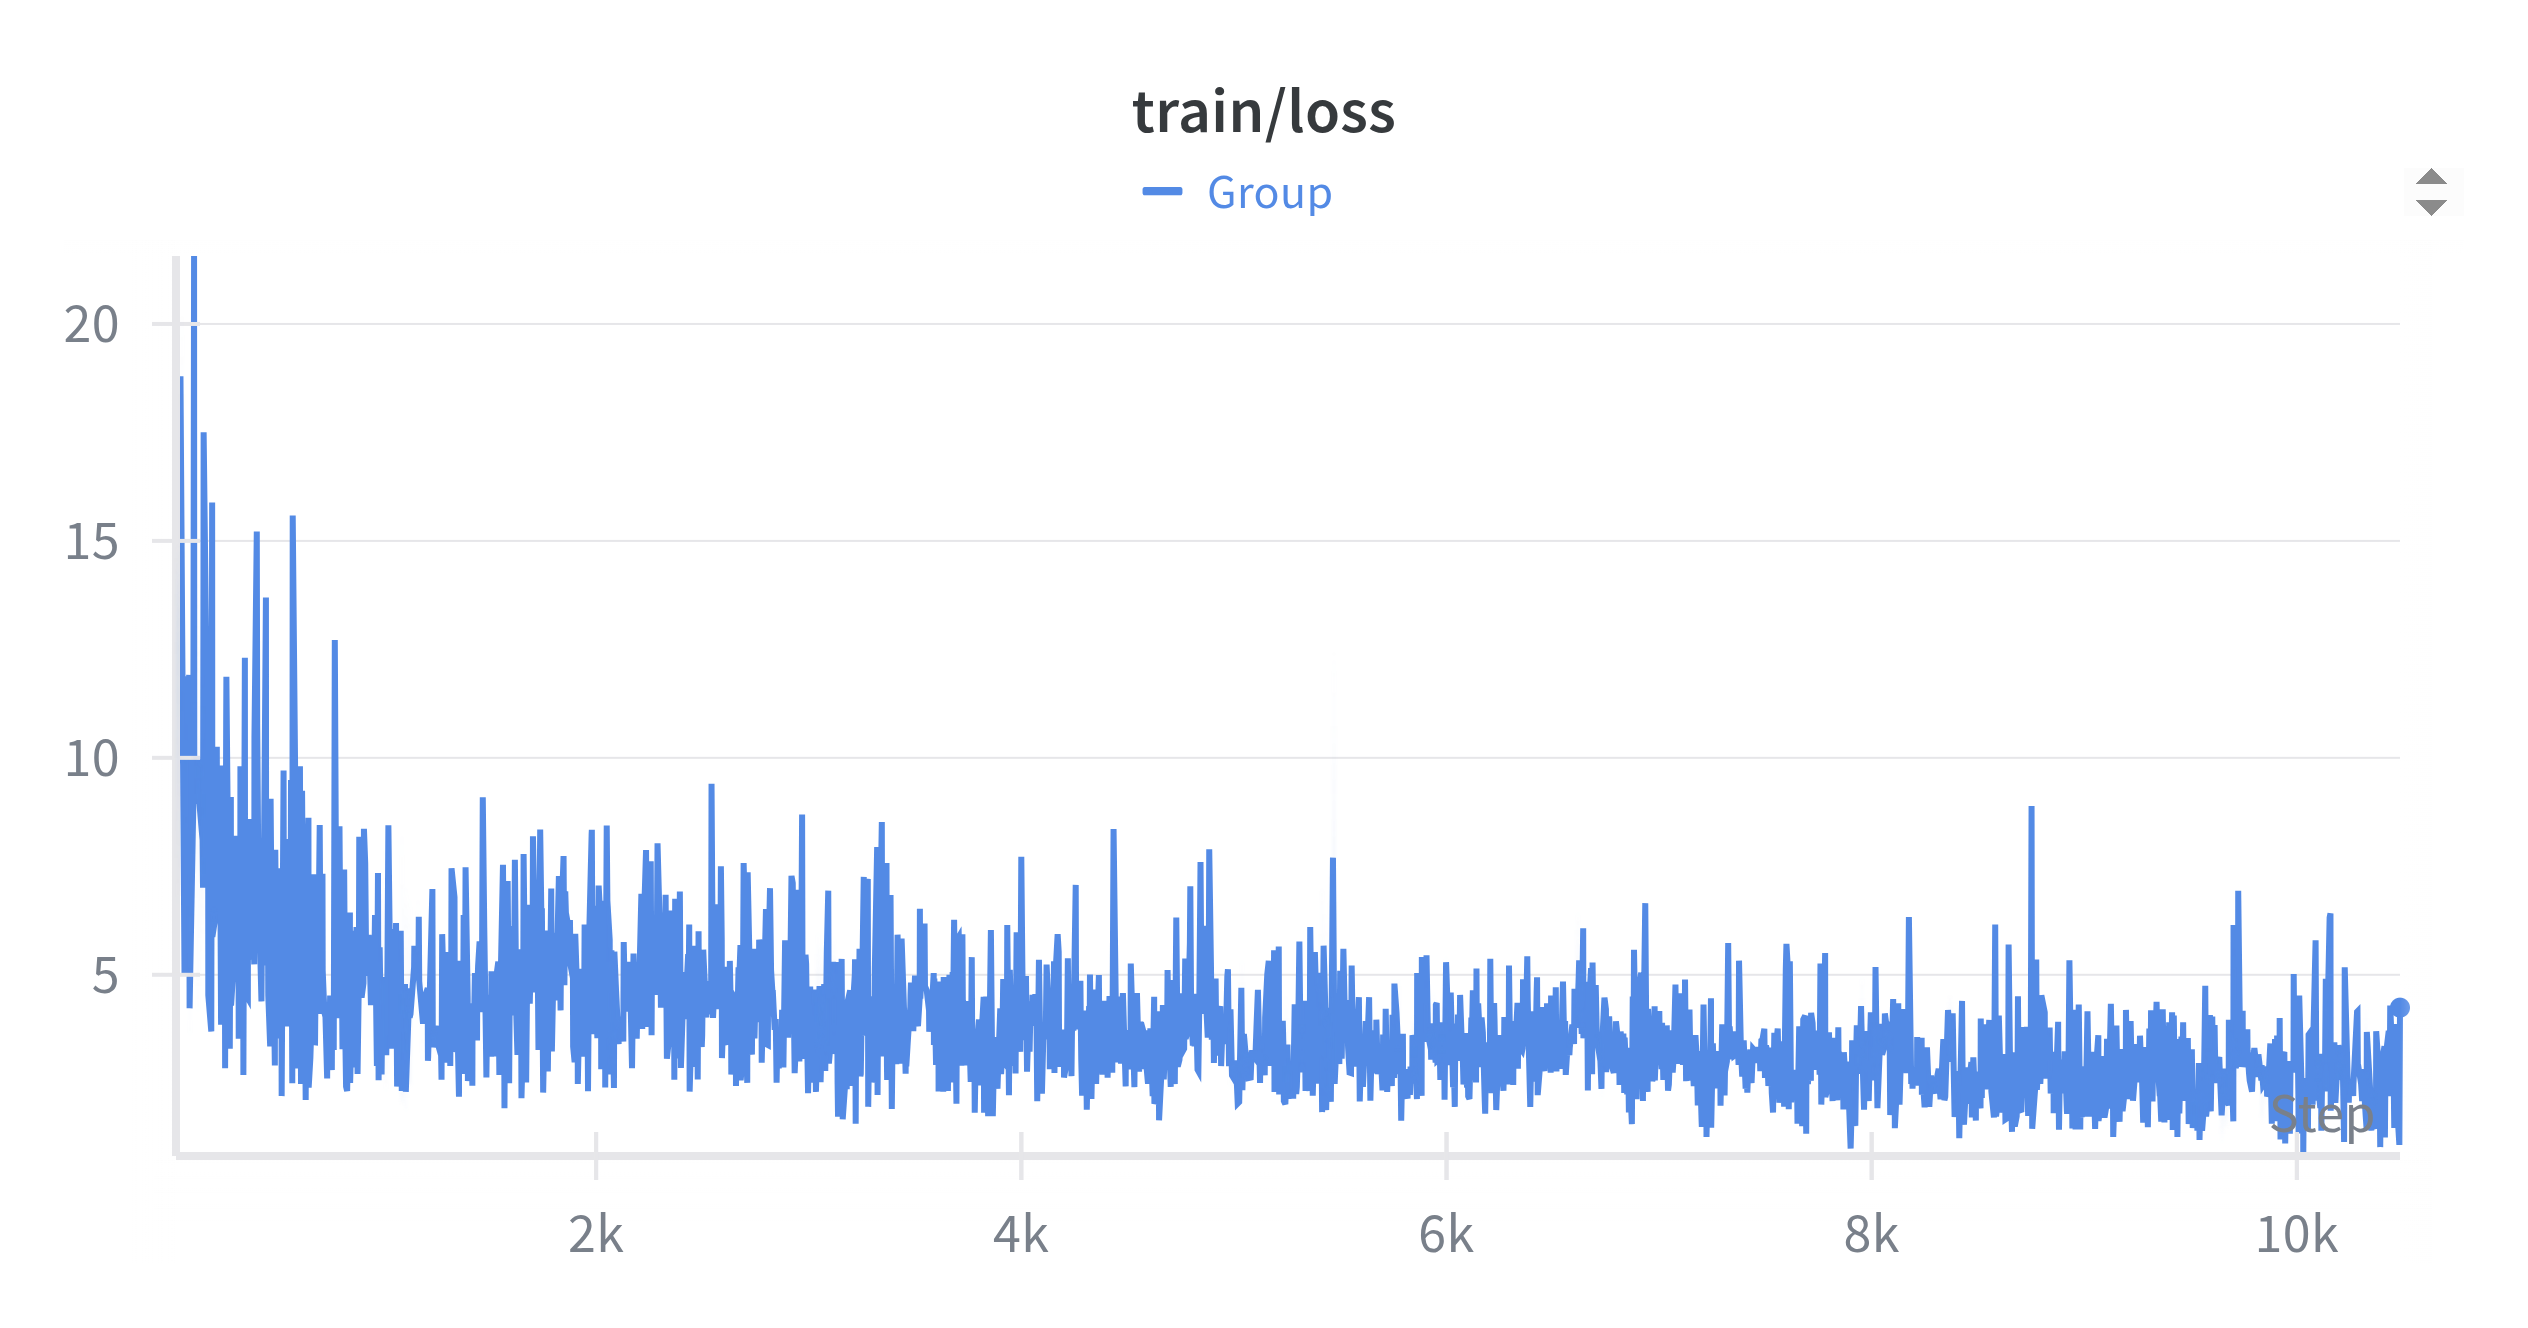
\includegraphics[width=0.7\linewidth]{photos/loss ppo - raw - 3 - rand.png} % مسیر فایل عکس را جایگزین کنید
\caption{پاداش دوره \lr{PPO} \lr{--} پاداش بازدهی خامِ نرمال‌شده \lr{--} محیط‌های برداری (۳-محیط) \lr{--} دوره‌های تصادفی}
\label{tab:ppo-raw-3env-normal}
\end{figure}


\begin{table}[H]
\centering
\caption{نتایج \lr{PPO} \lr{--} پاداش لگاریتمی تعدیل‌شده \lr{--} محیط تک‌گانه \lr{--} دوره‌های عادی}
\label{tab:ppo-logrisk-1env-normal}
\begin{tabular}{l c}
\toprule
\lr{Metric} & \lr{Mean $\pm$ Std} \\
\midrule
\lr{Annualized Return [\%]} & \lr{24.38 $\pm$ 8.64} \\
\lr{Annualized Volatility [\%]} & \lr{20.52 $\pm$ 1.45} \\
\lr{Max Drawdown [\%]} & \lr{-25.03 $\pm$ 0.82} \\
\lr{Average Drawdown [\%]} & \lr{-6.26 $\pm$ 2.13} \\
\lr{Sharpe Ratio} & \lr{1.16 $\pm$ 0.35} \\
\lr{Sortino Ratio} & \lr{1.55 $\pm$ 0.47} \\
\lr{Calmar Ratio} & \lr{0.97 $\pm$ 0.33} \\
\lr{Max Drawdown Duration (days)} & \lr{192.00 $\pm$ 113.68} \\
\lr{Number of Trades} & \lr{127.80 $\pm$ 47.99} \\
\bottomrule
\end{tabular}
\end{table}

\begin{figure}[H]
\centering
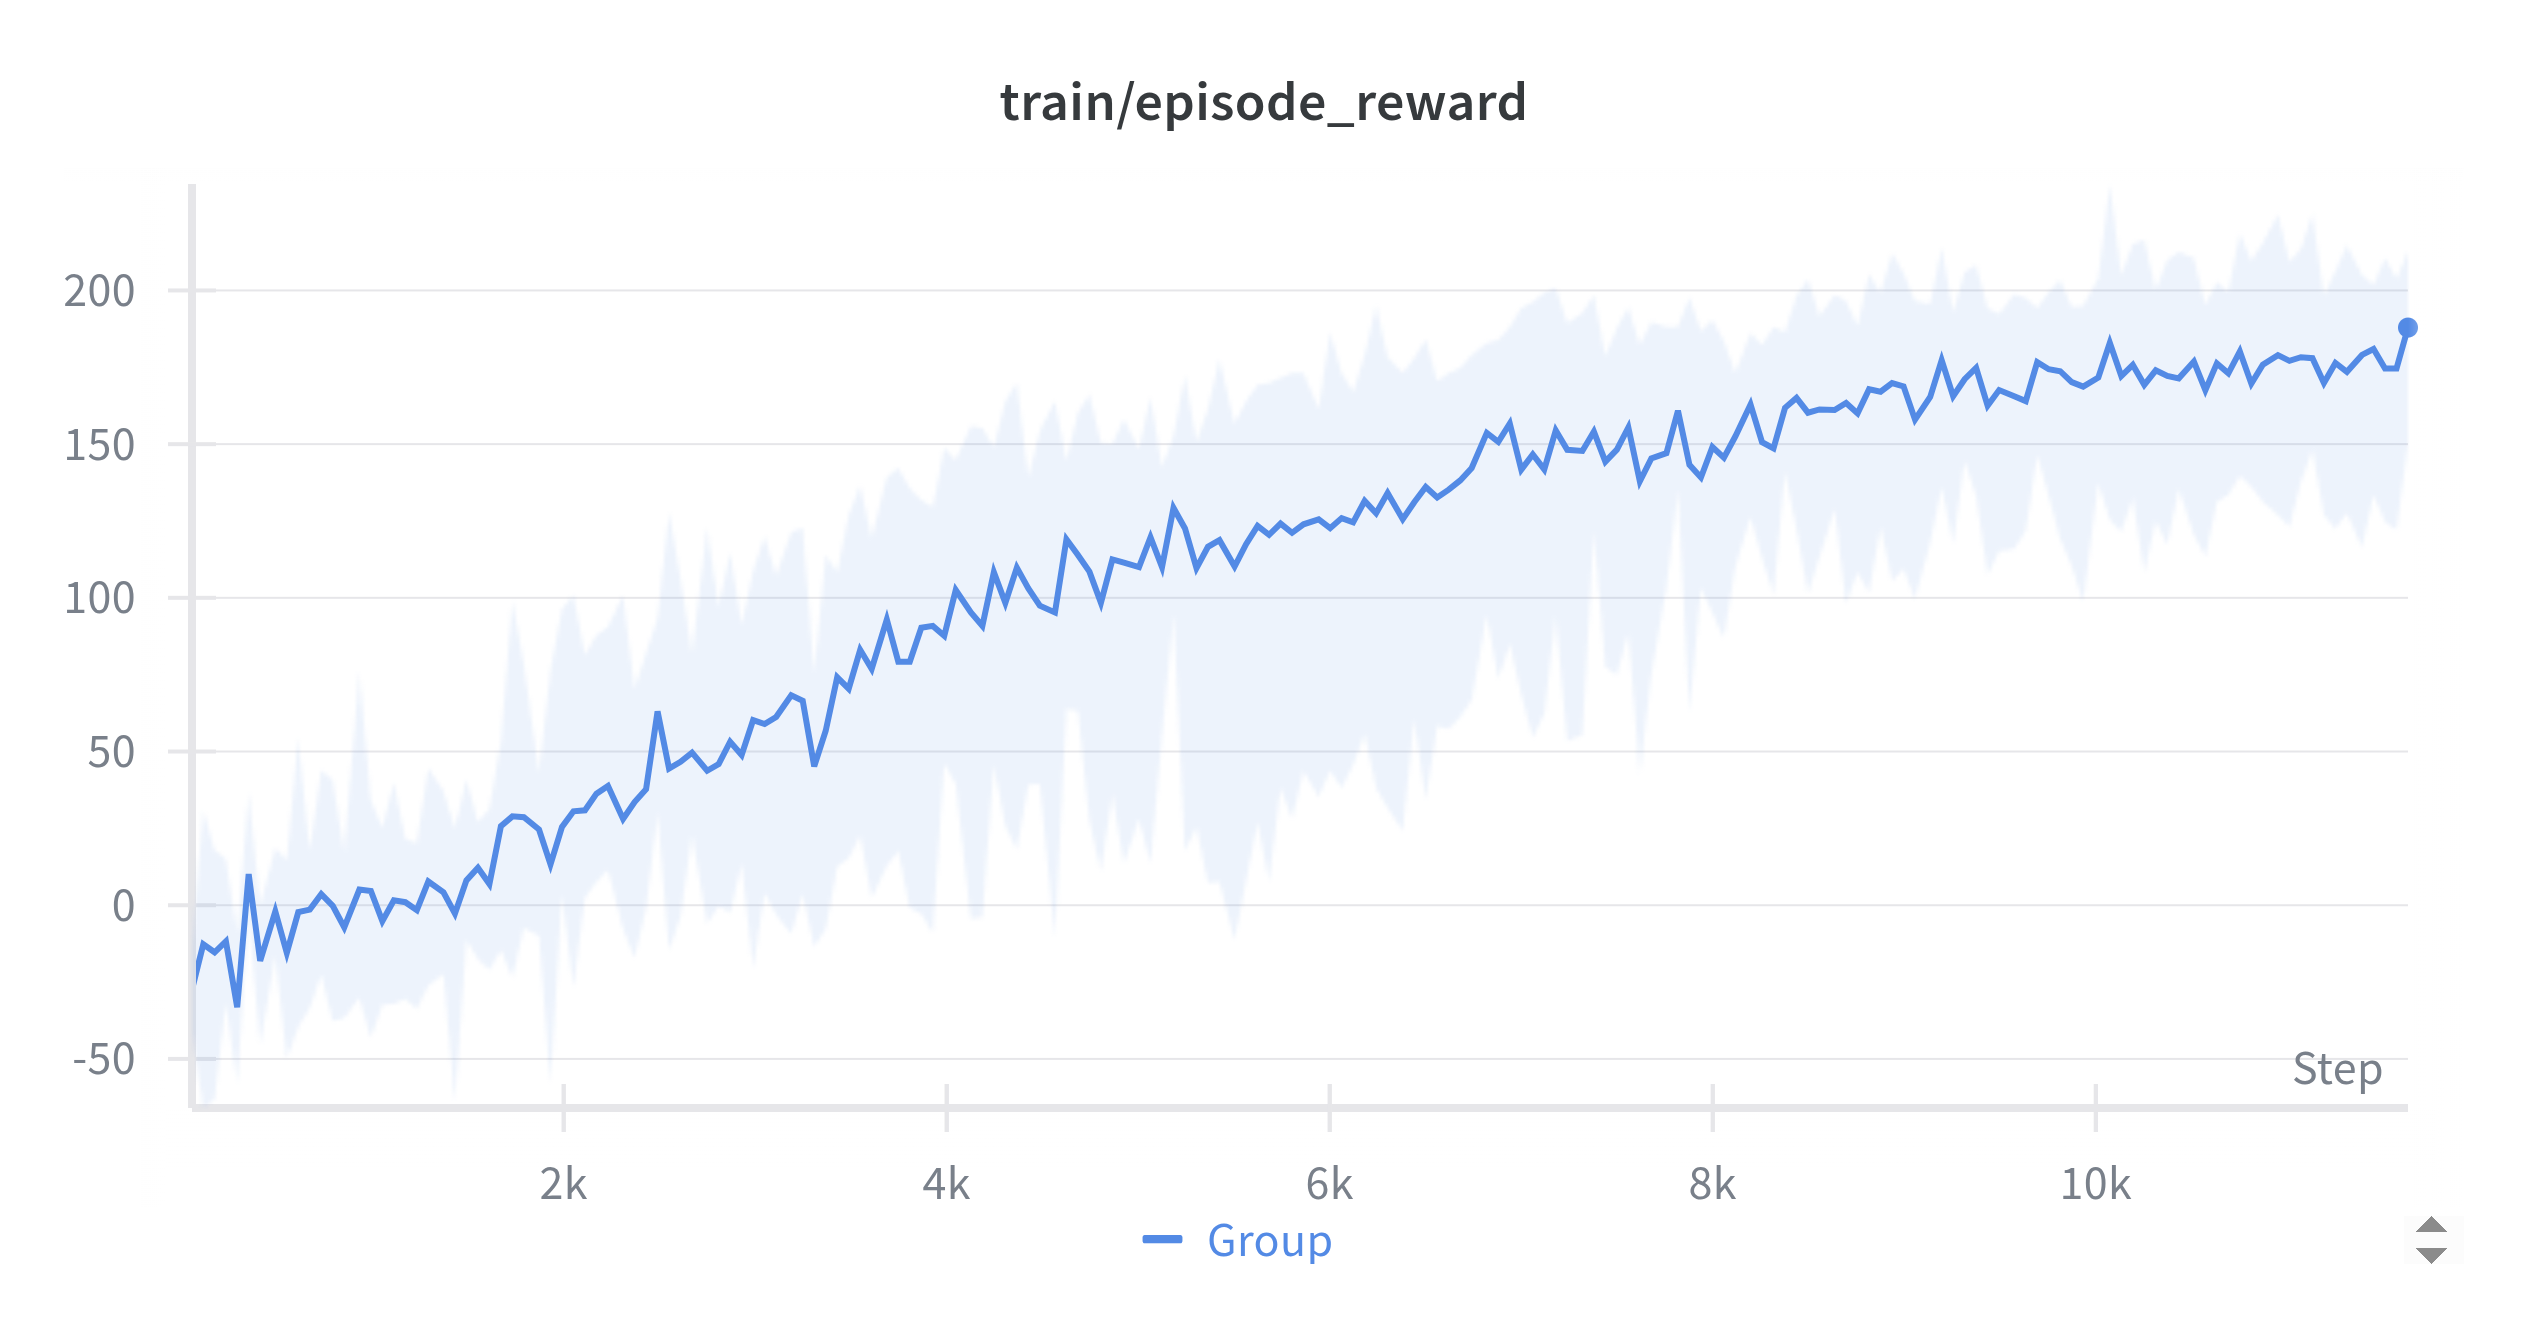
\includegraphics[width=0.7\linewidth]{photos/rew ppo - log - 1 - norm.png}
\caption{پاداش دوره \lr{PPO} \lr{--} پاداش لگاریتمی تعدیل‌شده \lr{--} محیط تک‌گانه \lr{--} دوره‌های عادی}
\label{fig:ppo-raw-1env-normal}
\end{figure}


\begin{figure}[H]
\centering
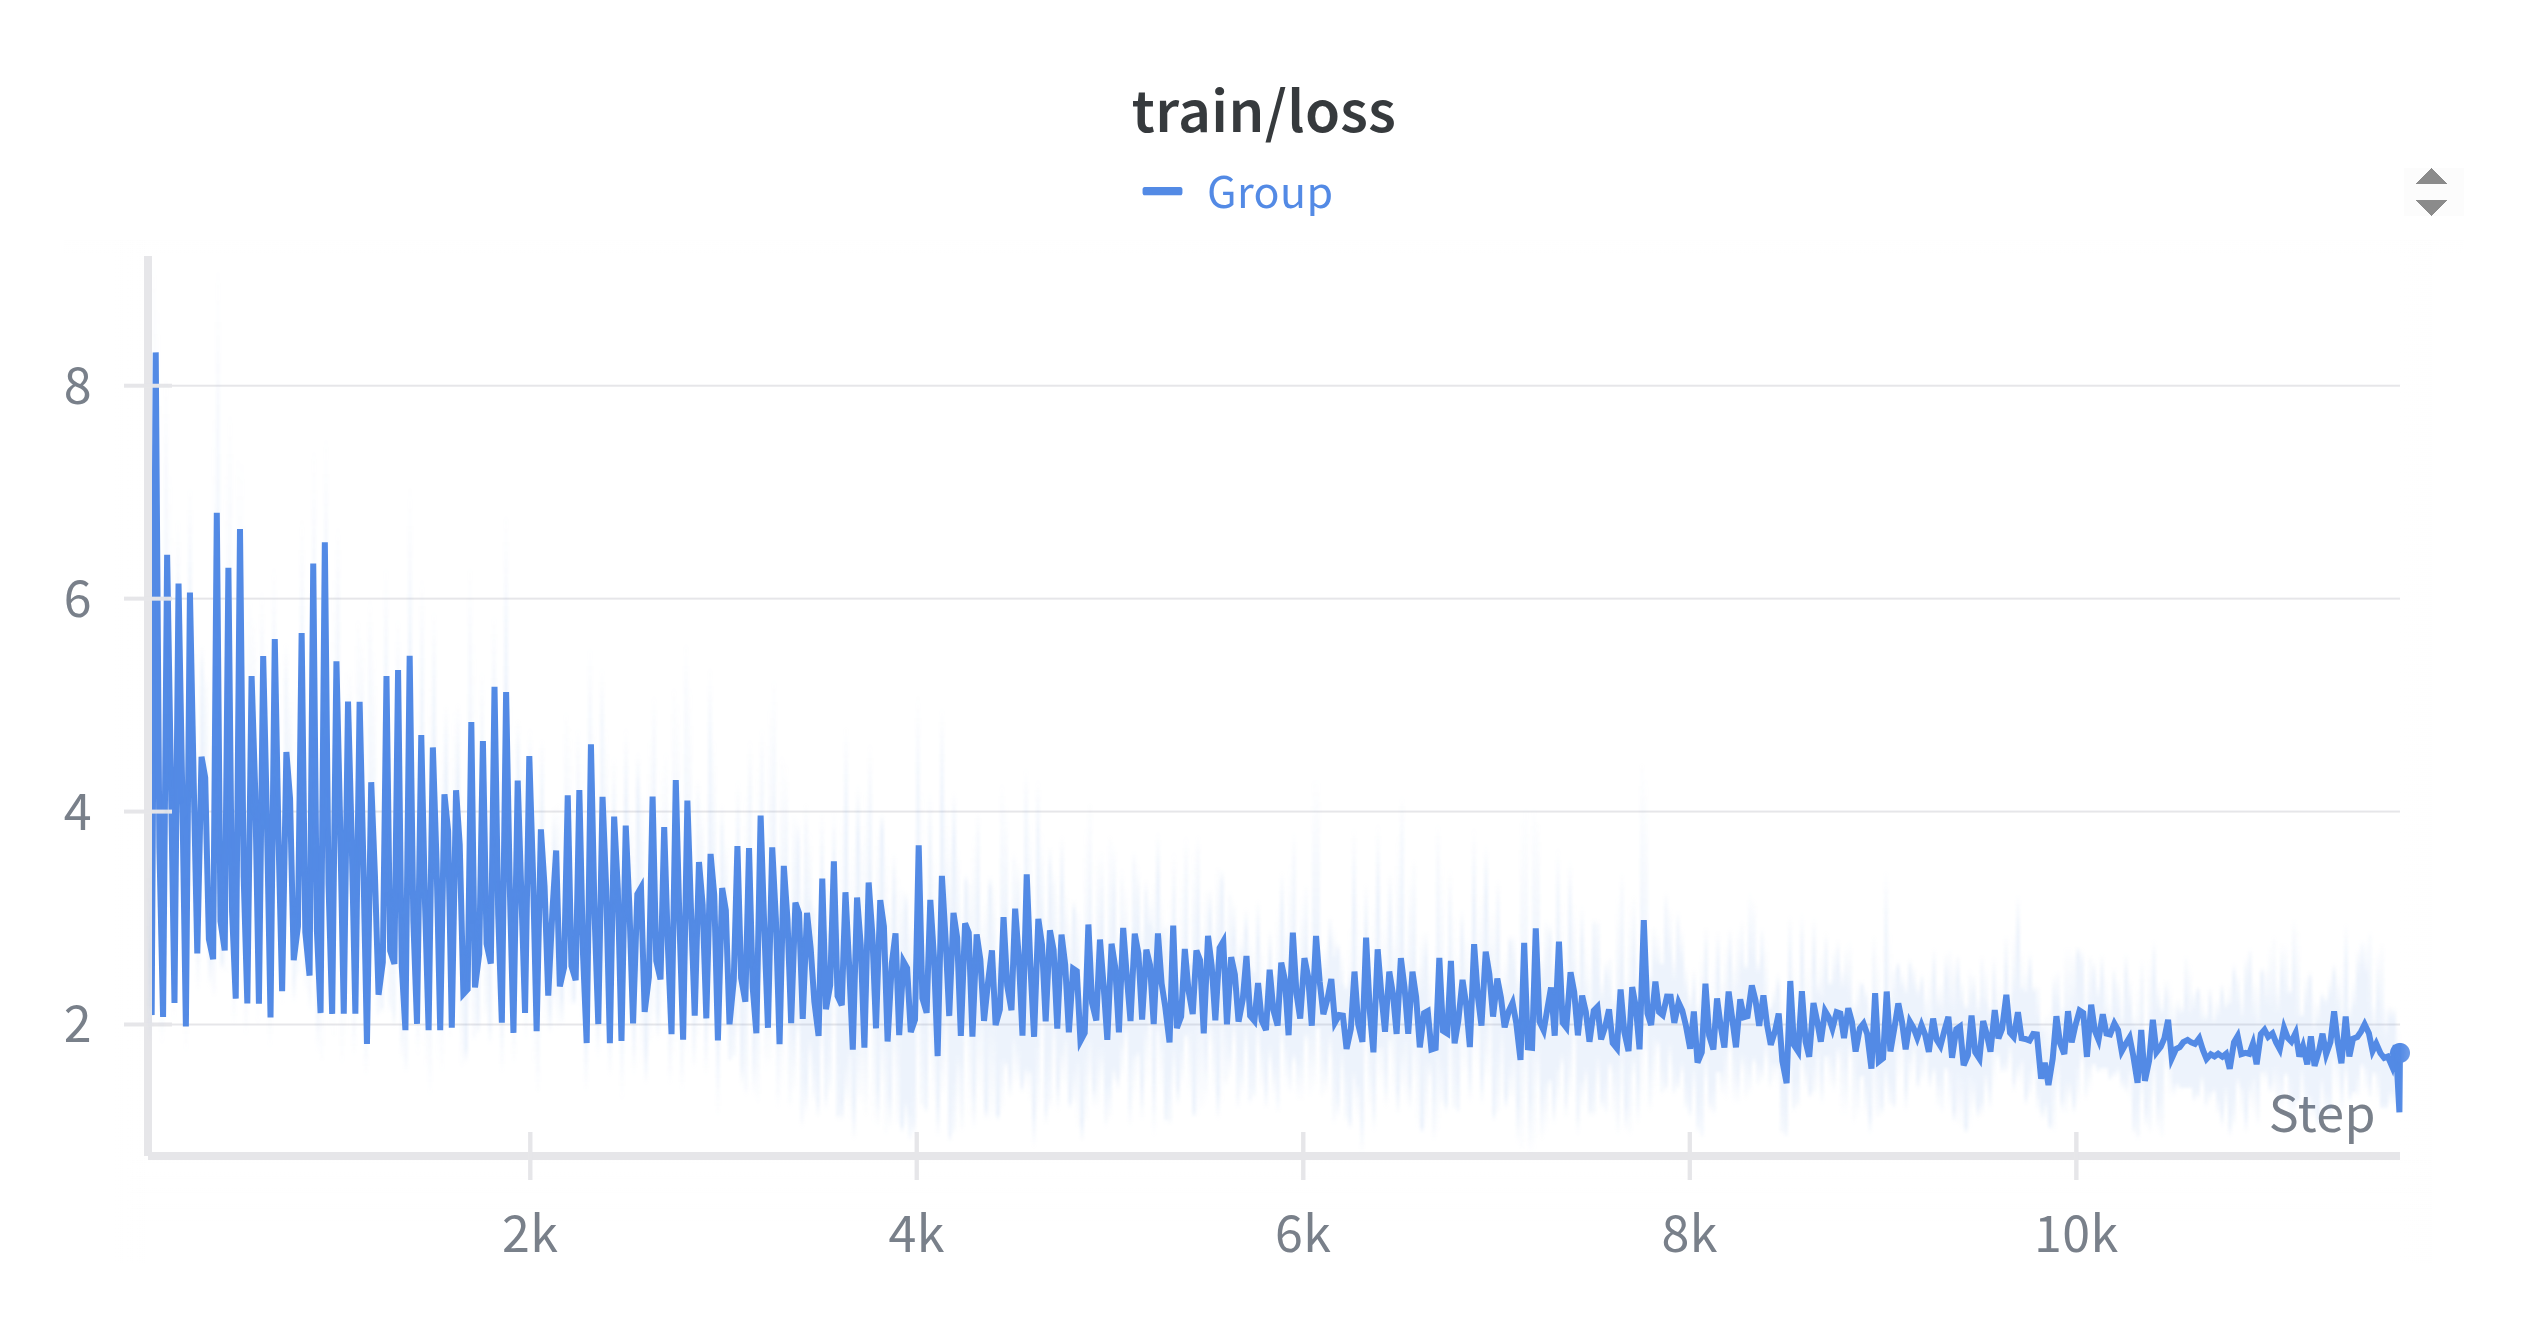
\includegraphics[width=0.7\linewidth]{photos/loss ppo - log - 1 - norm.png}
\caption{هزینه آموزش \lr{PPO} \lr{--} پاداش لگاریتمی تعدیل‌شده\lr{--} محیط تک‌گانه \lr{--} دوره‌های عادی}
\label{fig:ppo-raw-1env-normal}
\end{figure}



\begin{table}[H]
\centering
\caption{نتایج \lr{PPO} \lr{--} پاداش پاداش لگاریتمی تعدیل‌شده \lr{--} محیط‌های برداری (۳-محیط) \lr{--} دوره‌های عادی}
\label{tab:ppo-logrisk-3env-normal}
\begin{tabular}{l c}
\toprule
\lr{Metric} & \lr{Mean $\pm$ Std} \\
\midrule
\lr{Annualized Return [\%]} & \lr{21.97 $\pm$ 8.12} \\
\lr{Annualized Volatility [\%]} & \lr{20.84 $\pm$ 1.39} \\
\lr{Max Drawdown [\%]} & \lr{-25.33 $\pm$ 0.92} \\
\lr{Average Drawdown [\%]} & \lr{-6.44 $\pm$ 2.55} \\
\lr{Sharpe Ratio} & \lr{1.05 $\pm$ 0.31} \\
\lr{Sortino Ratio} & \lr{1.40 $\pm$ 0.40} \\
\lr{Calmar Ratio} & \lr{0.86 $\pm$ 0.30} \\
\lr{Max Drawdown Duration (days)} & \lr{214.50 $\pm$ 134.69} \\
\lr{Number of Trades} & \lr{135.75 $\pm$ 38.51} \\
\bottomrule
\end{tabular}
\end{table}

\begin{figure}[H]
\centering
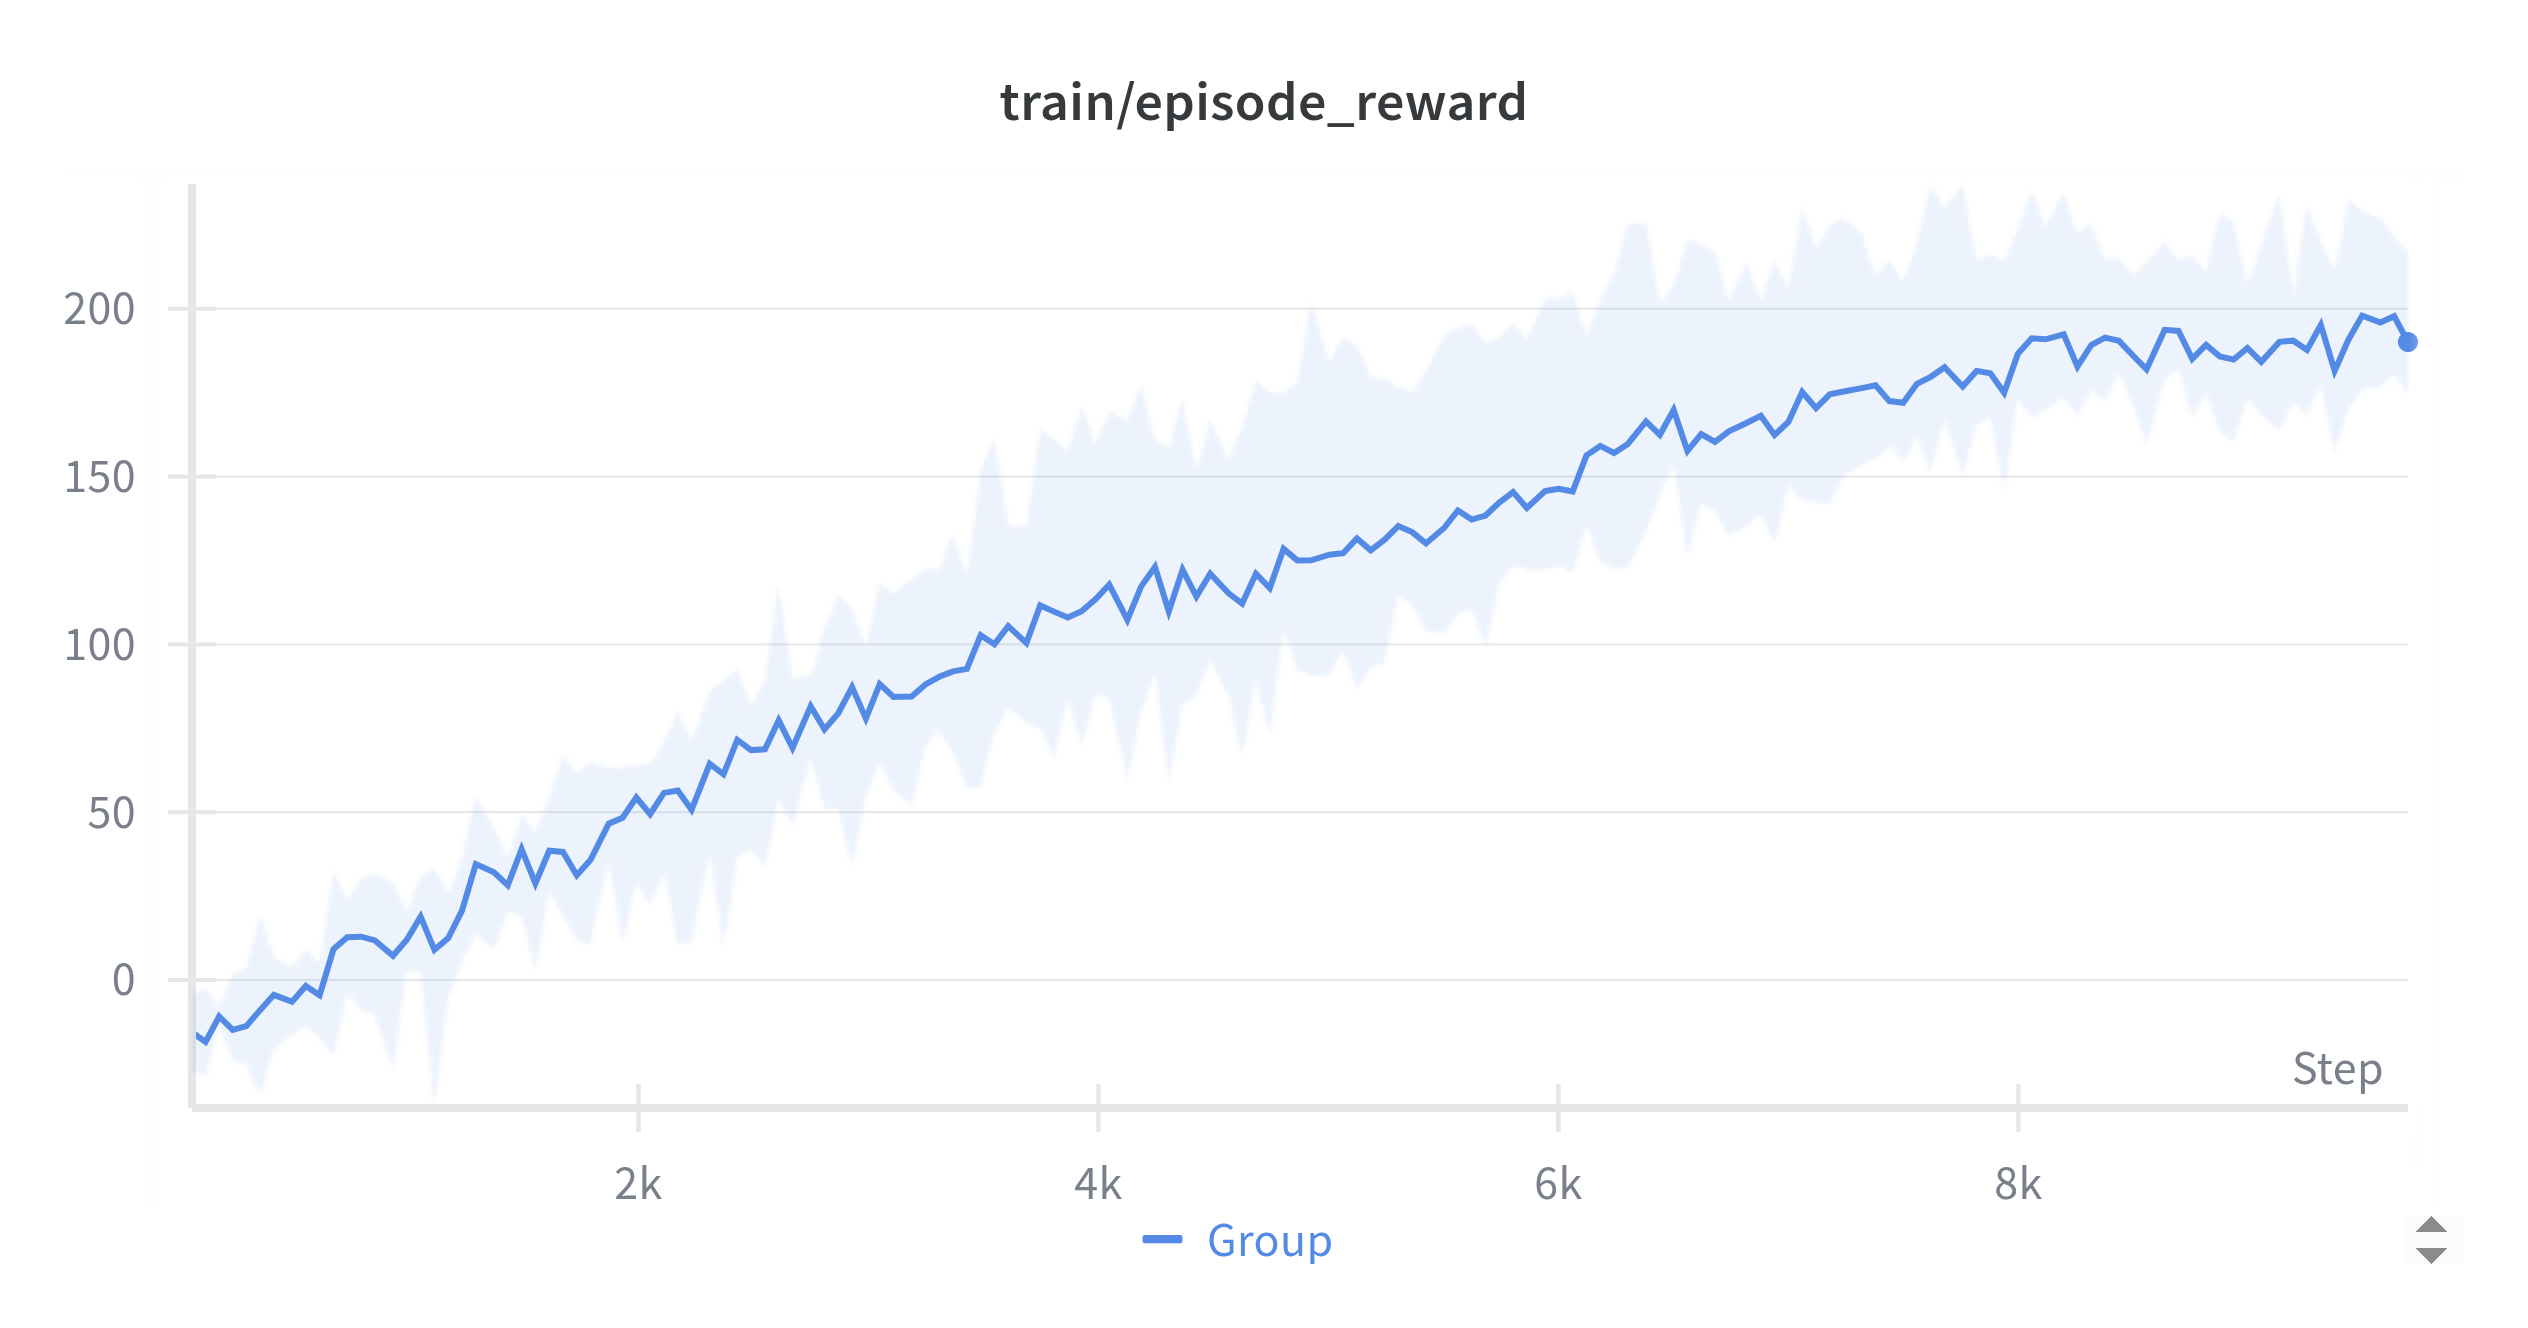
\includegraphics[width=0.7\linewidth]{photos/rew ppo - log - 3 - norm.png}
\caption{پاداش دوره \lr{PPO} \lr{--} پاداش لگاریتمی تعدیل‌شده \lr{--} محیط‌های برداری (۳-محیط) \lr{--} دوره‌های عادی}
\label{fig:ppo-raw-1env-normal}
\end{figure}


\begin{figure}[H]
\centering
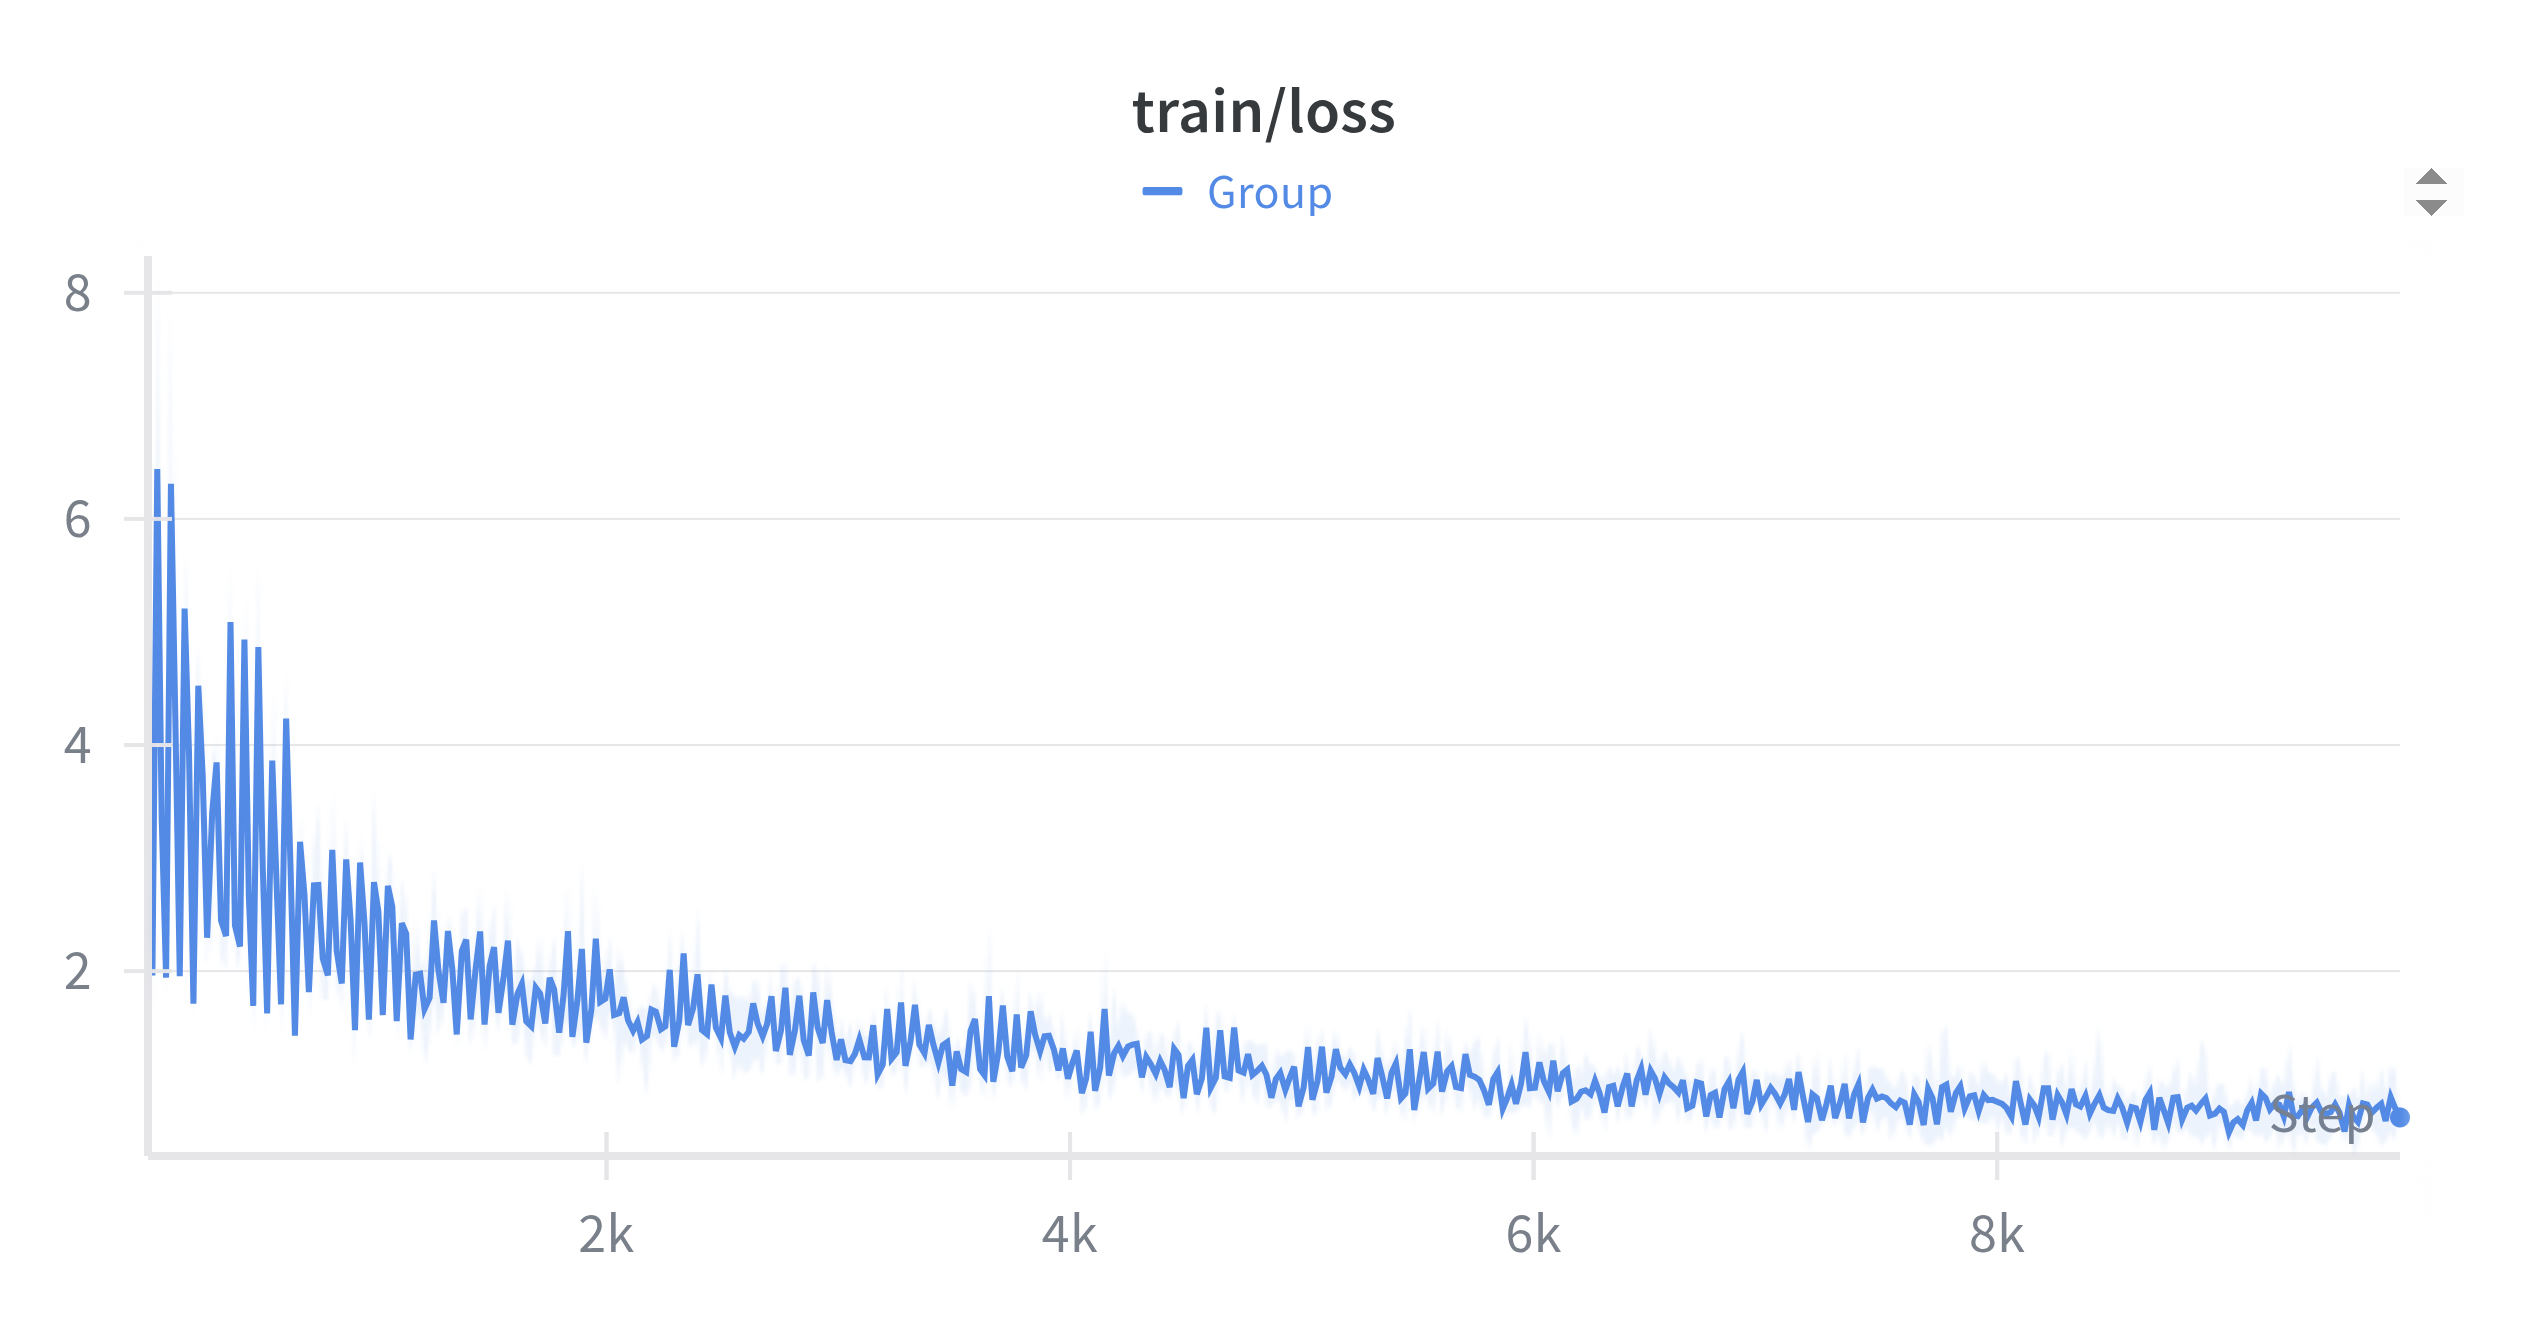
\includegraphics[width=0.7\linewidth]{photos/loss ppo - log - 3 - norm.png}
\caption{هزینه آموزش \lr{PPO} \lr{--} پاداش لگاریتمی تعدیل‌شده \lr{--} محیط‌های برداری (۳-محیط) \lr{--} دوره‌های عادی}
\label{fig:ppo-raw-1env-normal}
\end{figure}




\begin{table}[H]
\centering
\caption{نتایج \lr{RPPO} \lr{--} پاداش بازدهی خامِ نرمال‌شده \lr{--} محیط تک‌گانه \lr{--} دوره‌های عادی}
\label{tab:rppo-raw-1env-normal}
\begin{tabular}{l c}
\toprule
\lr{Metric} & \lr{Mean $\pm$ Std} \\
\midrule
\lr{Annualized Return [\%]} & \lr{22.67 $\pm$ 5.21} \\
\lr{Annualized Volatility [\%]} & \lr{19.68 $\pm$ 1.73} \\
\lr{Max Drawdown [\%]} & \lr{-24.53 $\pm$ 1.58} \\
\lr{Average Drawdown [\%]} & \lr{-5.85 $\pm$ 1.62} \\
\lr{Sharpe Ratio} & \lr{1.14 $\pm$ 0.23} \\
\lr{Sortino Ratio} & \lr{1.53 $\pm$ 0.31} \\
\lr{Calmar Ratio} & \lr{0.93 $\pm$ 0.21} \\
\lr{Max Drawdown Duration (days)} & \lr{175.00 $\pm$ 99.07} \\
\lr{Number of Trades} & \lr{85.30 $\pm$ 30.01} \\
\bottomrule
\end{tabular}
\end{table}

\begin{figure}[H]
\centering
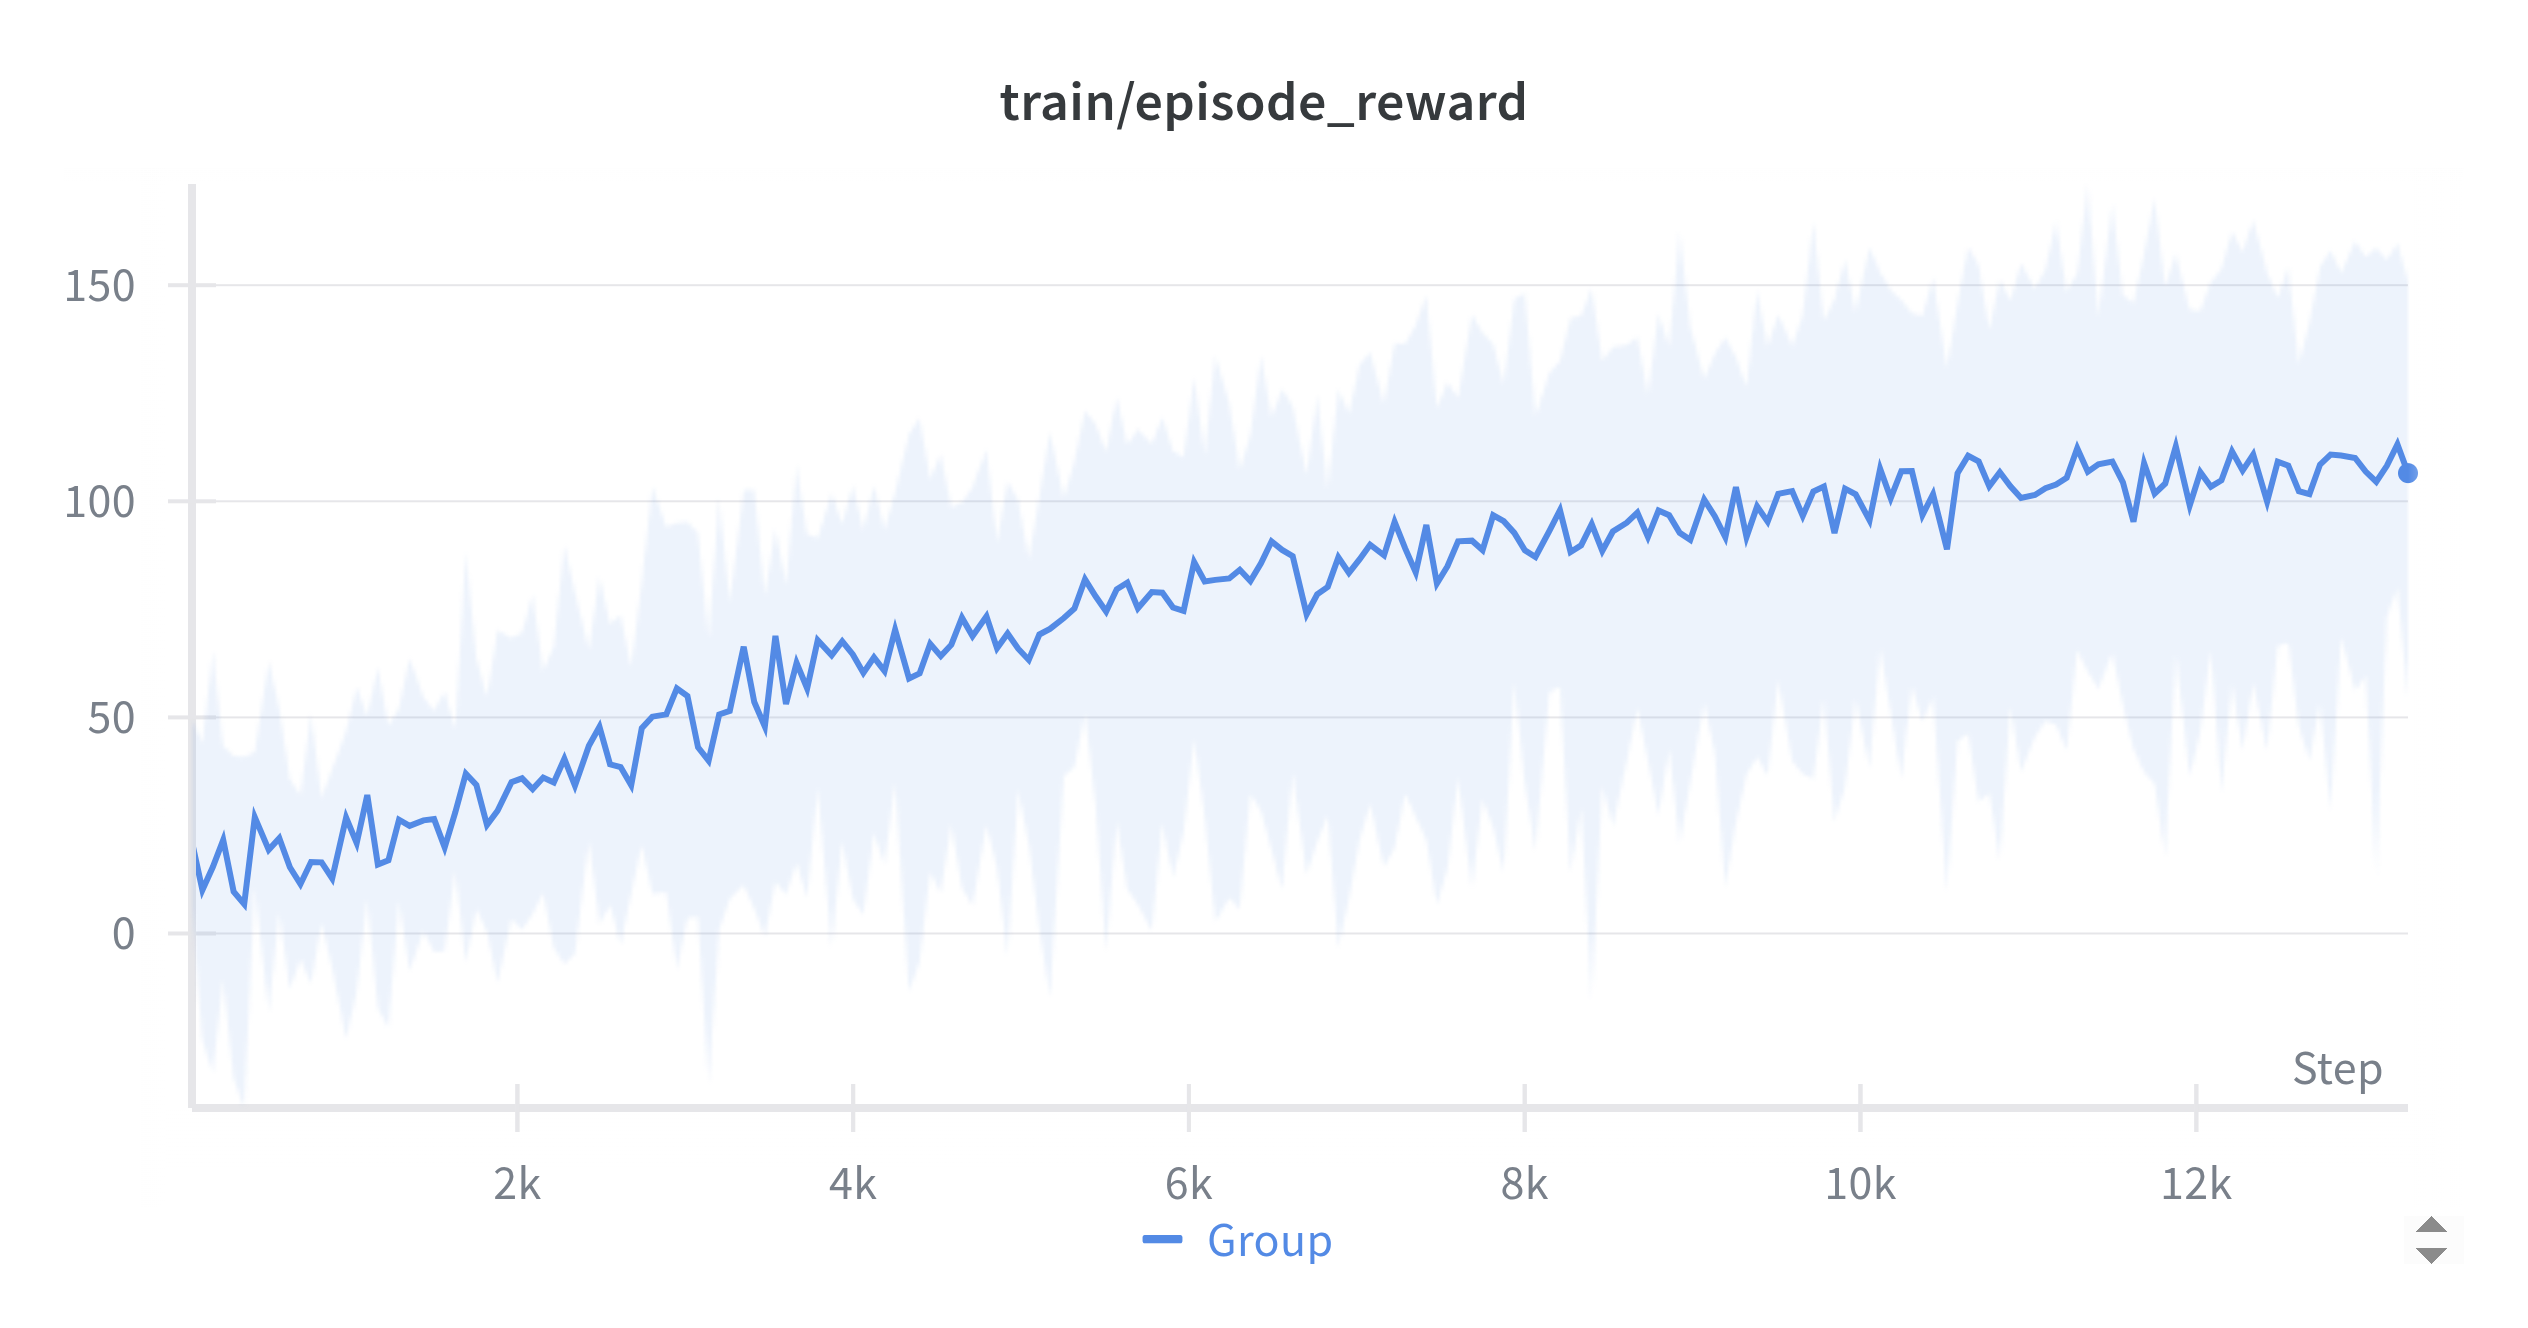
\includegraphics[width=0.7\linewidth]{photos/rew rppo - raw - 1 - norm.png}
\caption{پاداش دوره \lr{RPPO} \lr{--} پاداش بازدهی خامِ نرمال‌شده \lr{--} محیط تک‌گانه \lr{--} دوره‌های عادی}
\label{fig:ppo-raw-1env-normal}
\end{figure}


\begin{figure}[H]
\centering
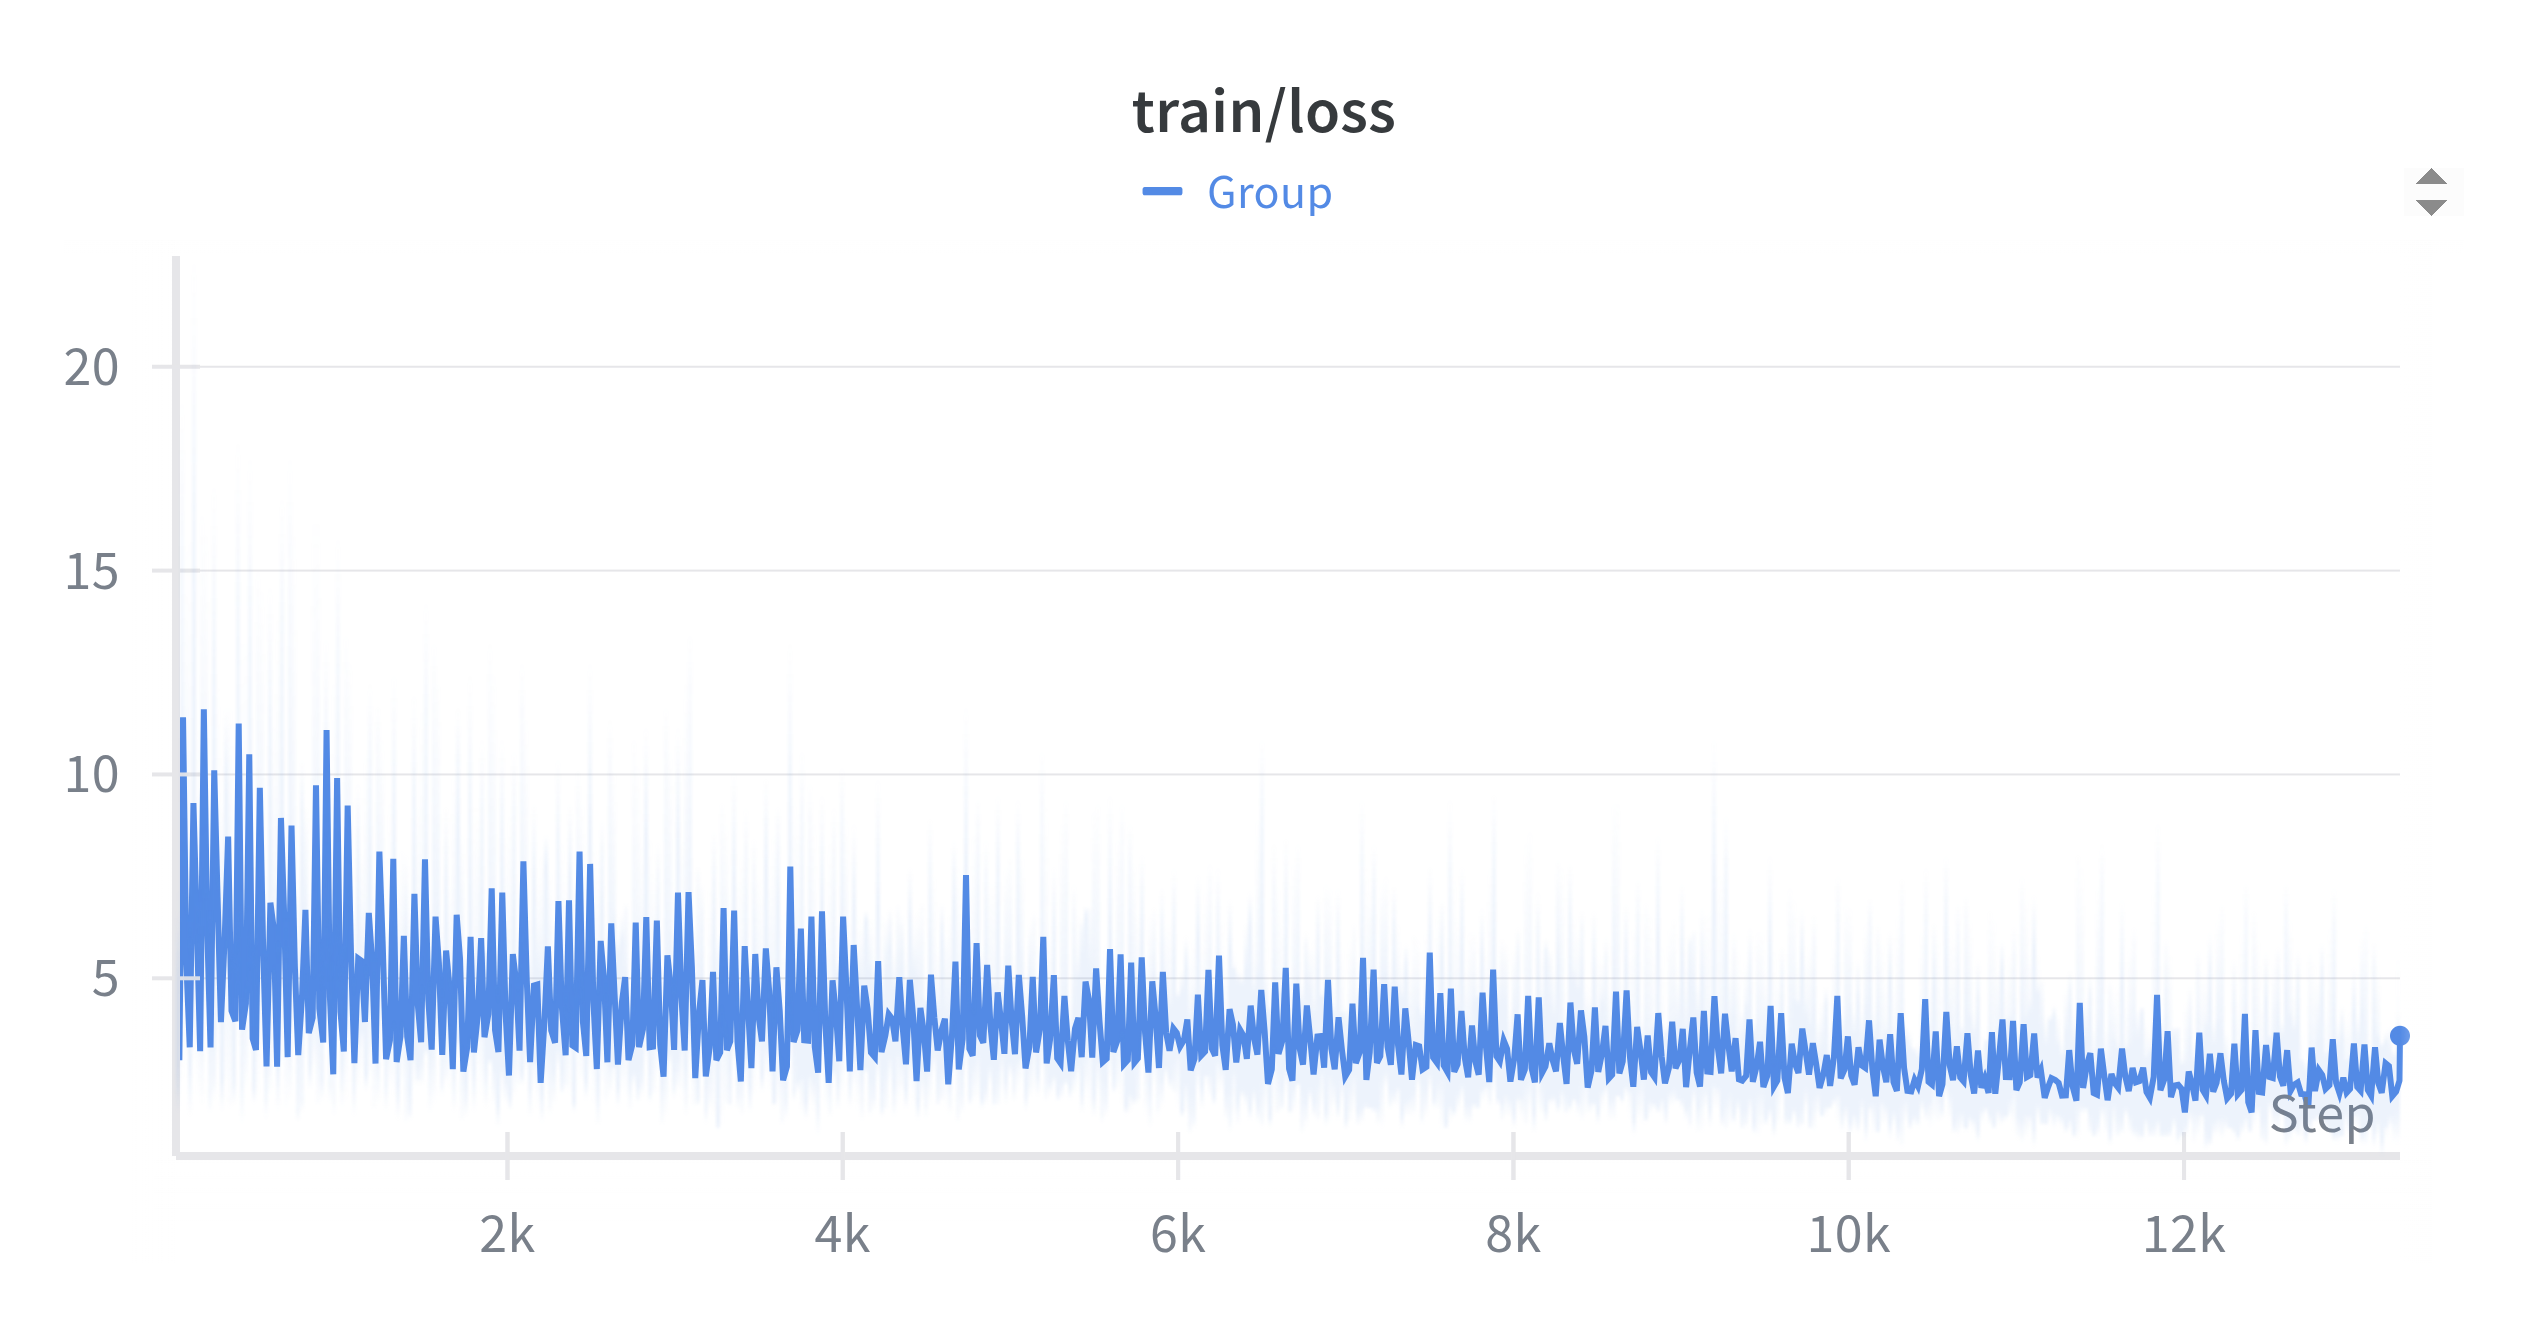
\includegraphics[width=0.7\linewidth]{photos/loss rppo - raw - 1 - norm.png}
\caption{هزینه آموزش \lr{RPPO} \lr{--} پاداش بازدهی خامِ نرمال‌شده \lr{--} محیط تک‌گانه \lr{--} دوره‌های عادی}
\label{fig:ppo-raw-1env-normal}
\end{figure}


\begin{table}[H]
\centering
\caption{نتایج \lr{RPPO} \lr{--} پاداش بازدهی خامِ نرمال‌شده \lr{--} محیط تک‌گانه \lr{--} دوره‌های تصادفی}
\label{tab:rppo-raw-1env-random}
\begin{tabular}{l c}
\toprule
\lr{Metric} & \lr{Mean $\pm$ Std} \\
\midrule
\lr{Annualized Return [\%]} & \lr{22.05 $\pm$ 3.40} \\
\lr{Annualized Volatility [\%]} & \lr{19.05 $\pm$ 1.94} \\
\lr{Max Drawdown [\%]} & \lr{-24.13 $\pm$ 1.45} \\
\lr{Average Drawdown [\%]} & \lr{-5.57 $\pm$ 1.36} \\
\lr{Sharpe Ratio} & \lr{1.16 $\pm$ 0.20} \\
\lr{Sortino Ratio} & \lr{1.56 $\pm$ 0.26} \\
\lr{Calmar Ratio} & \lr{0.92 $\pm$ 0.16} \\
\lr{Max Drawdown Duration (days)} & \lr{142.33 $\pm$ 58.01} \\
\lr{Number of Trades} & \lr{112.17 $\pm$ 35.53} \\
\bottomrule
\end{tabular}
\end{table}


\begin{figure}[H]
\centering
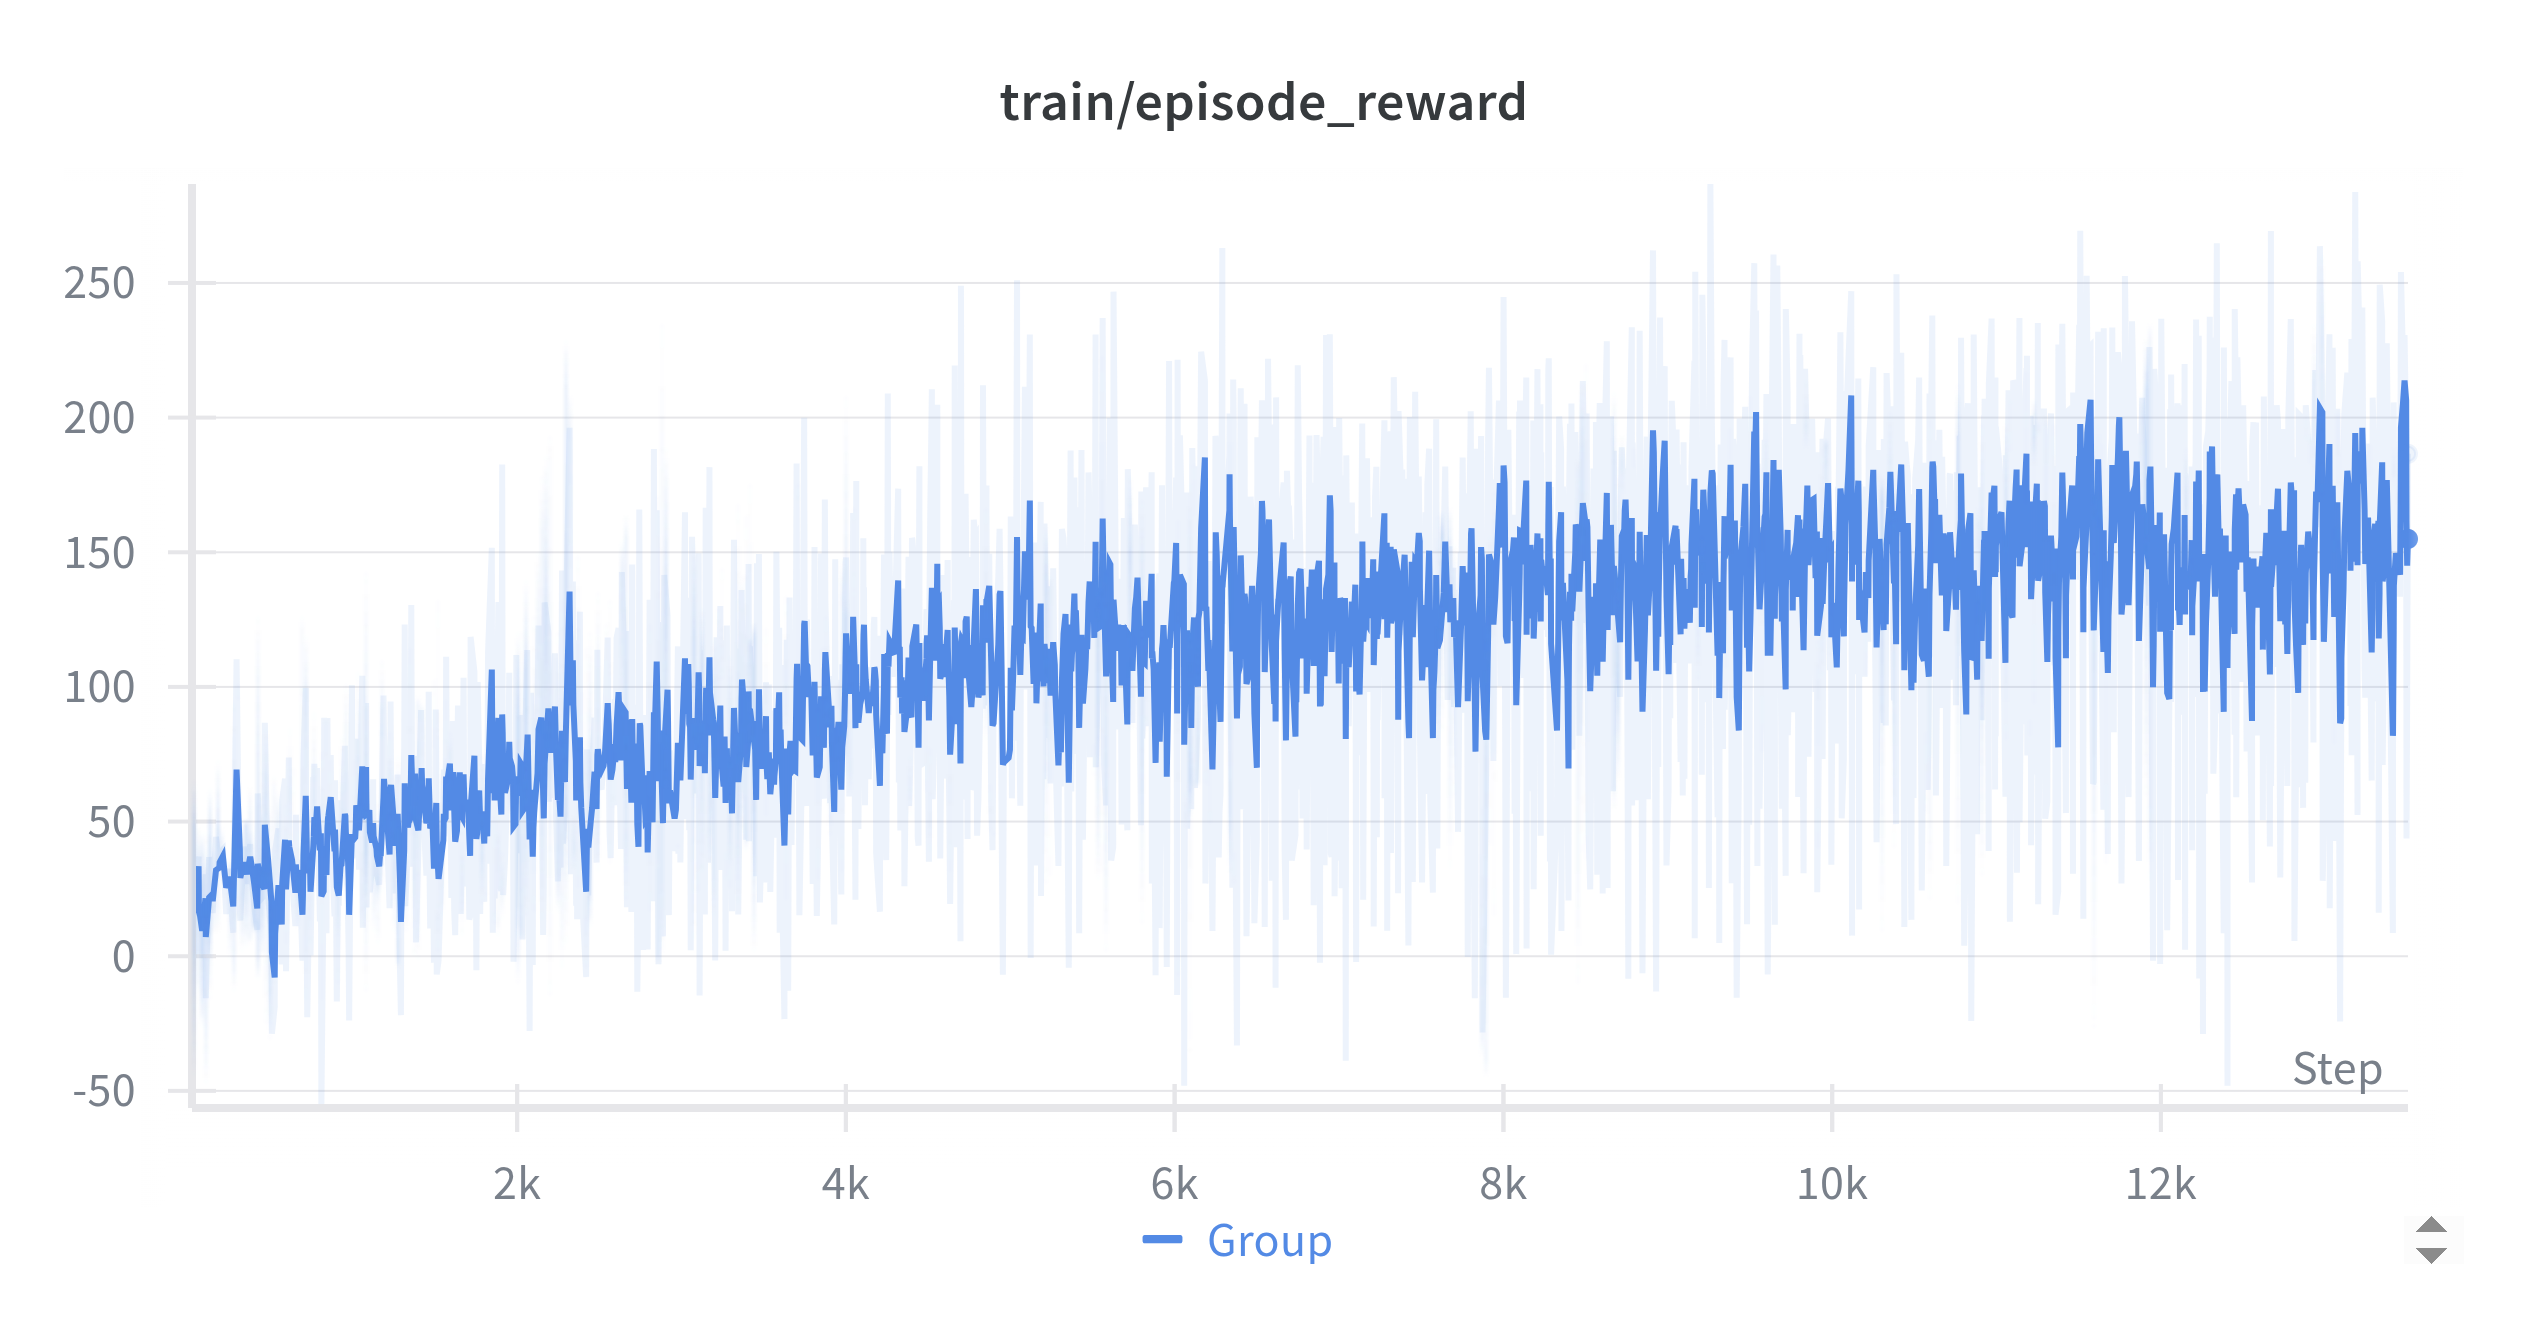
\includegraphics[width=0.7\linewidth]{photos/rew rppo - raw - 1 - rand.png}
\caption{پاداش دوره \lr{RPPO} \lr{--} پاداش بازدهی خامِ نرمال‌شده \lr{--} محیط تک‌گانه \lr{--} دوره‌های عادی}
\label{fig:ppo-raw-1env-normal}
\end{figure}


\begin{figure}[H]
\centering
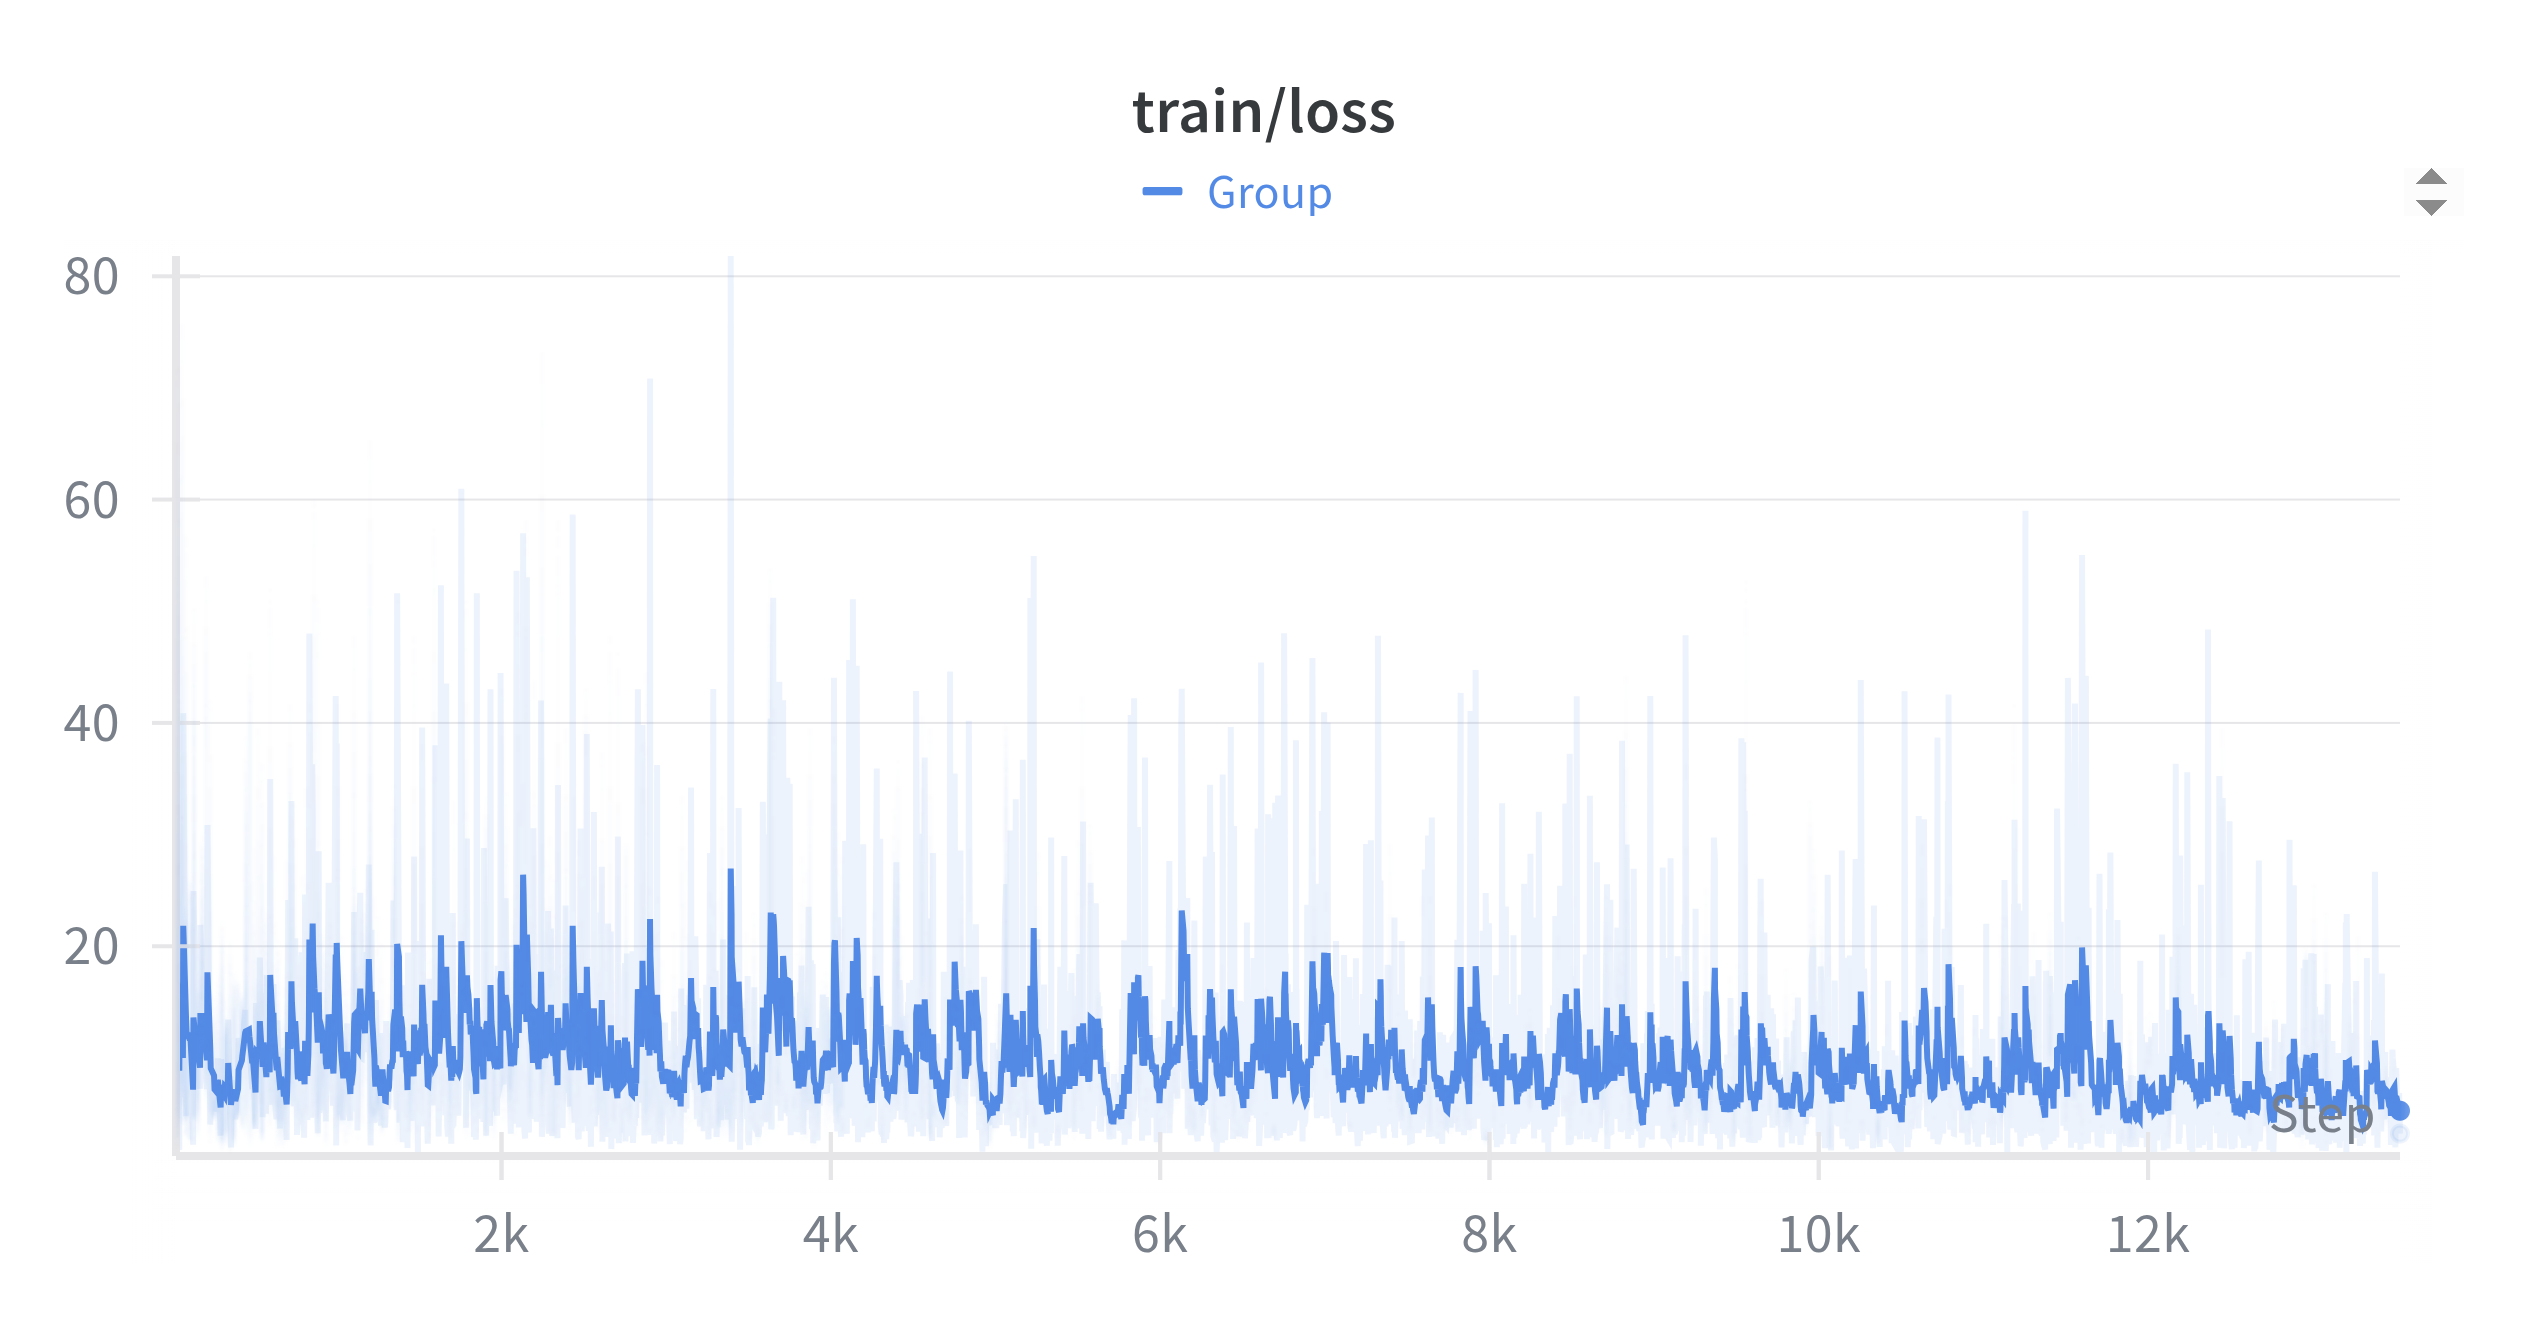
\includegraphics[width=0.7\linewidth]{photos/loss rppo - raw - 1 - rand.png}
\caption{هزینه آموزش \lr{RPPO} \lr{--} پاداش بازدهی خامِ نرمال‌شده \lr{--} محیط تک‌گانه \lr{--} دوره‌های عادی}
\label{fig:ppo-raw-1env-normal}
\end{figure}



\begin{table}[H]
\centering
\caption{نتایج \lr{RPPO} \lr{--} پاداش بازدهی خامِ نرمال‌شده \lr{--} محیط‌های برداری (۳-محیط) \lr{--} دوره‌های عادی}
\label{tab:rppo-raw-3env-normal}
\begin{tabular}{l c}
\toprule
\lr{Metric} & \lr{Mean $\pm$ Std} \\
\midrule
\lr{Annualized Return [\%]} & \lr{28.62 $\pm$ 2.23} \\
\lr{Annualized Volatility [\%]} & \lr{19.60 $\pm$ 1.69} \\
\lr{Max Drawdown [\%]} & \lr{-25.11 $\pm$ 2.97} \\
\lr{Average Drawdown [\%]} & \lr{-4.48 $\pm$ 0.40} \\
\lr{Sharpe Ratio} & \lr{1.39 $\pm$ 0.04} \\
\lr{Sortino Ratio} & \lr{1.83 $\pm$ 0.11} \\
\lr{Calmar Ratio} & \lr{1.14 $\pm$ 0.06} \\
\lr{Max Drawdown Duration (days)} & \lr{99.80 $\pm$ 8.84} \\
\lr{Number of Trades} & \lr{89.80 $\pm$ 36.19} \\
\bottomrule
\end{tabular}
\end{table}

\begin{figure}[H]
\centering
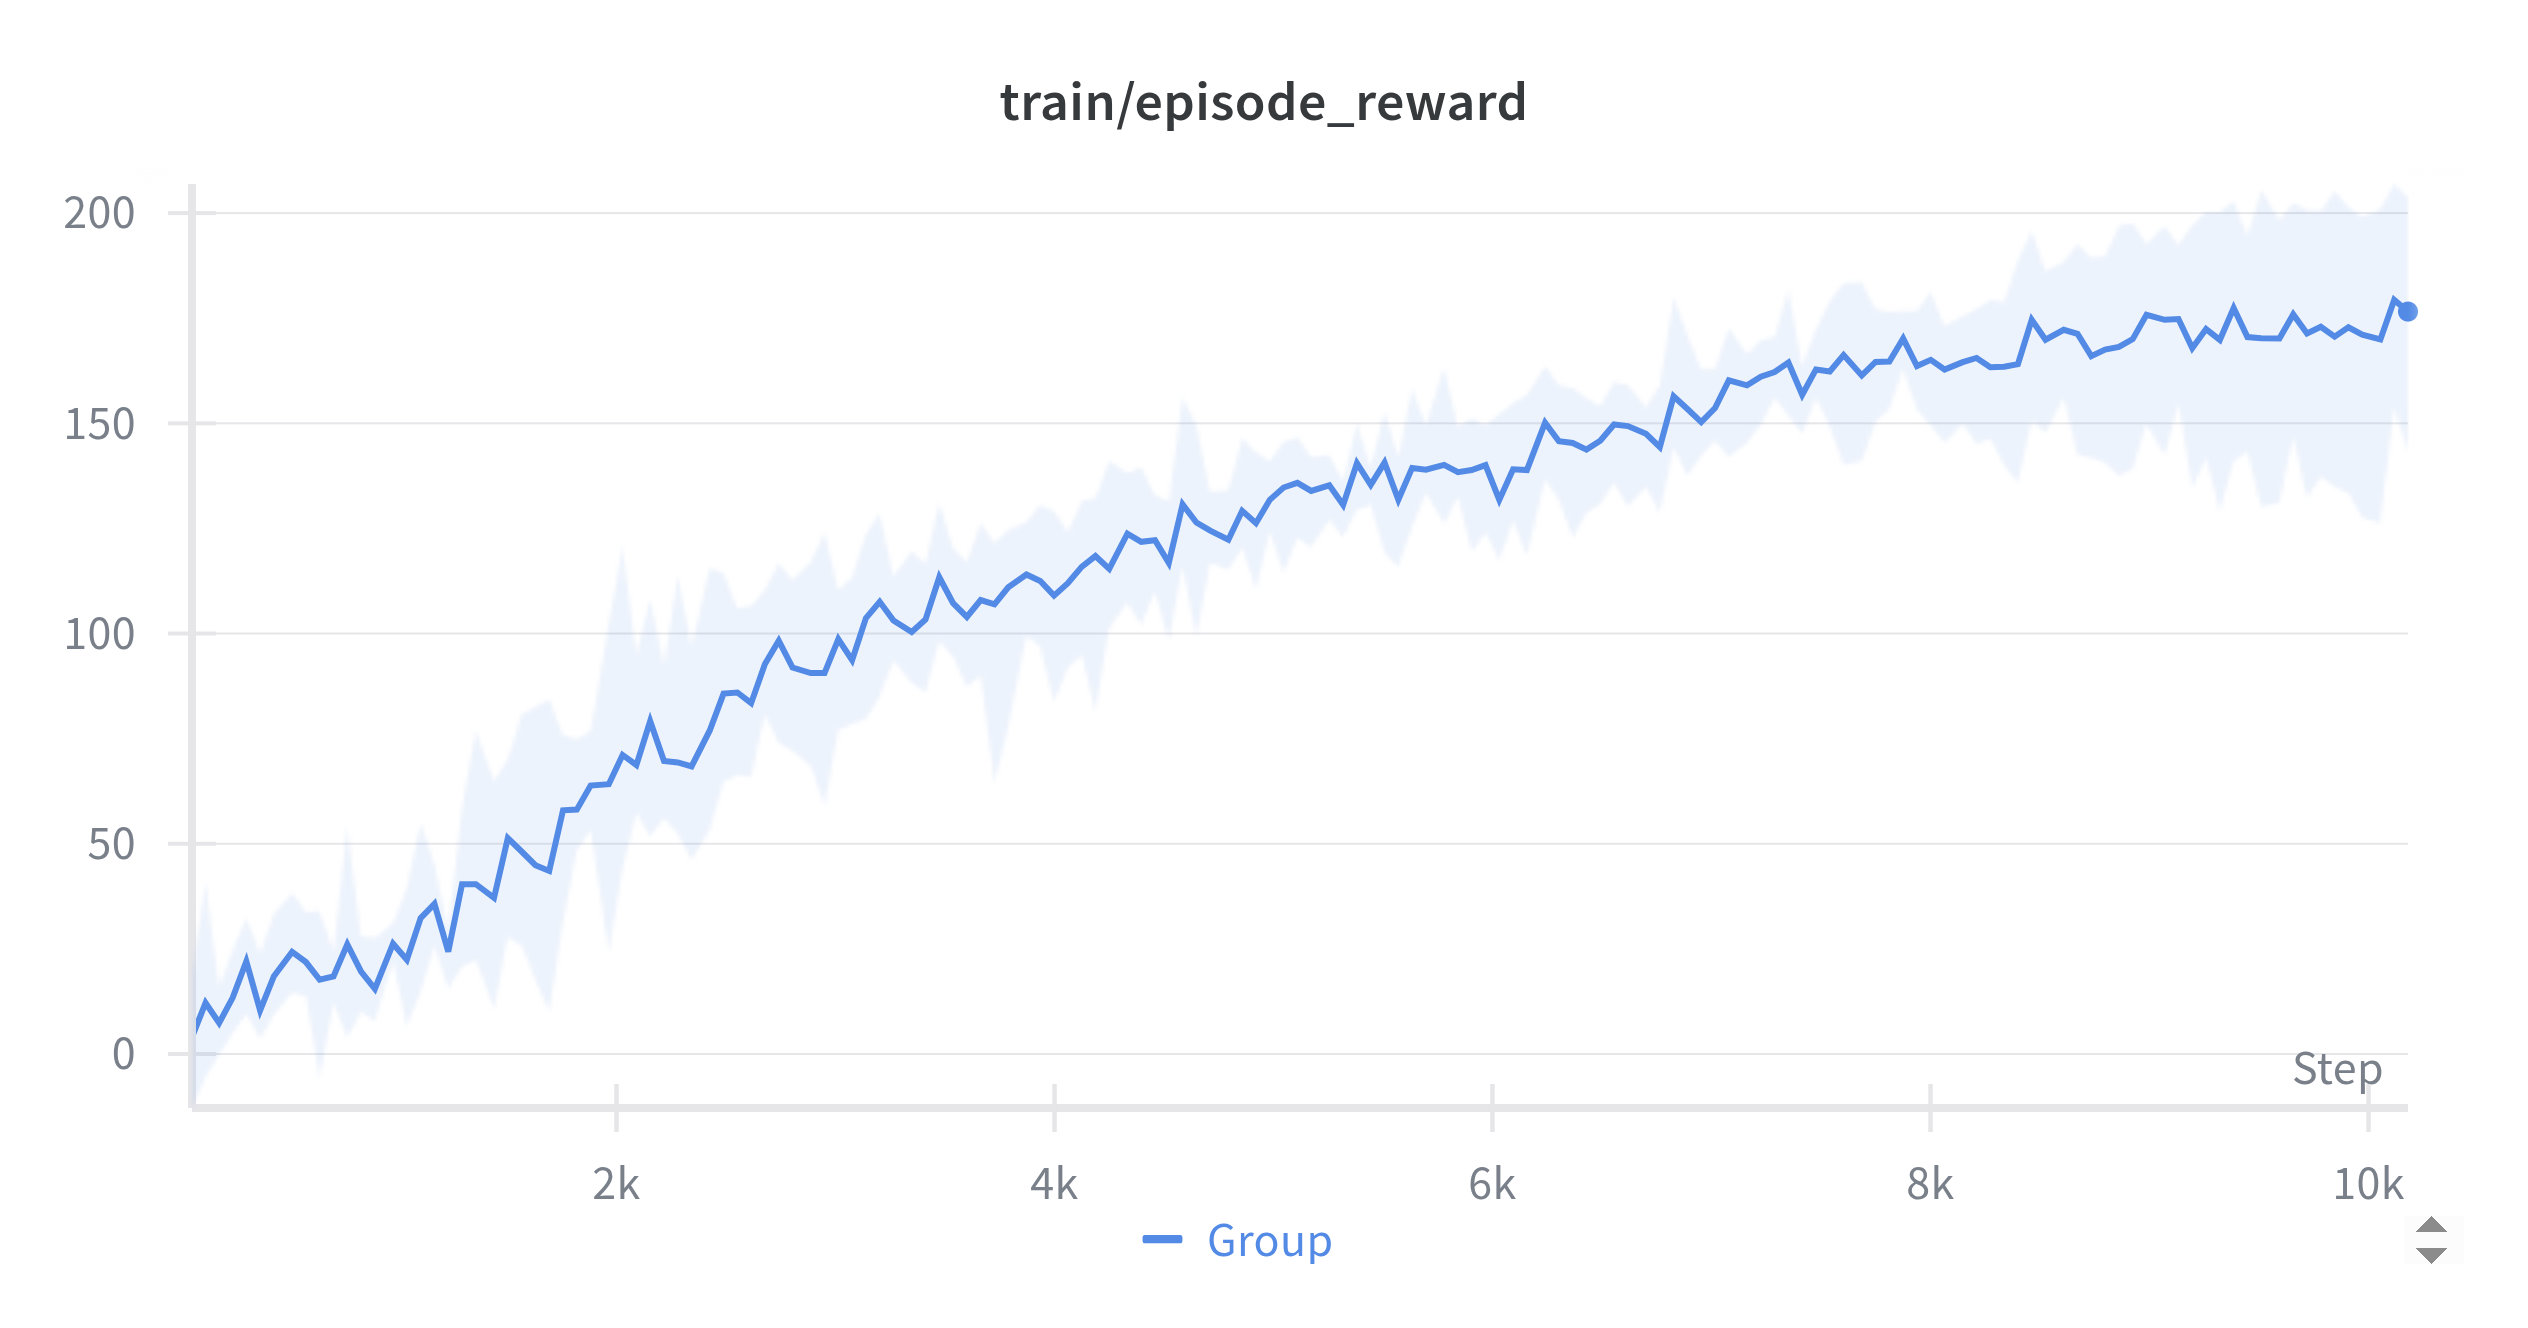
\includegraphics[width=0.7\linewidth]{photos/rew rppo - raw - 3 - norm.png}
\caption{پاداش دوره \lr{RPPO} \lr{--} پاداش بازدهی خامِ نرمال‌شده \lr{--} محیط تک‌گانه \lr{--} دوره‌های عادی}
\label{fig:ppo-raw-1env-normal}
\end{figure}


\begin{figure}[H]
\centering
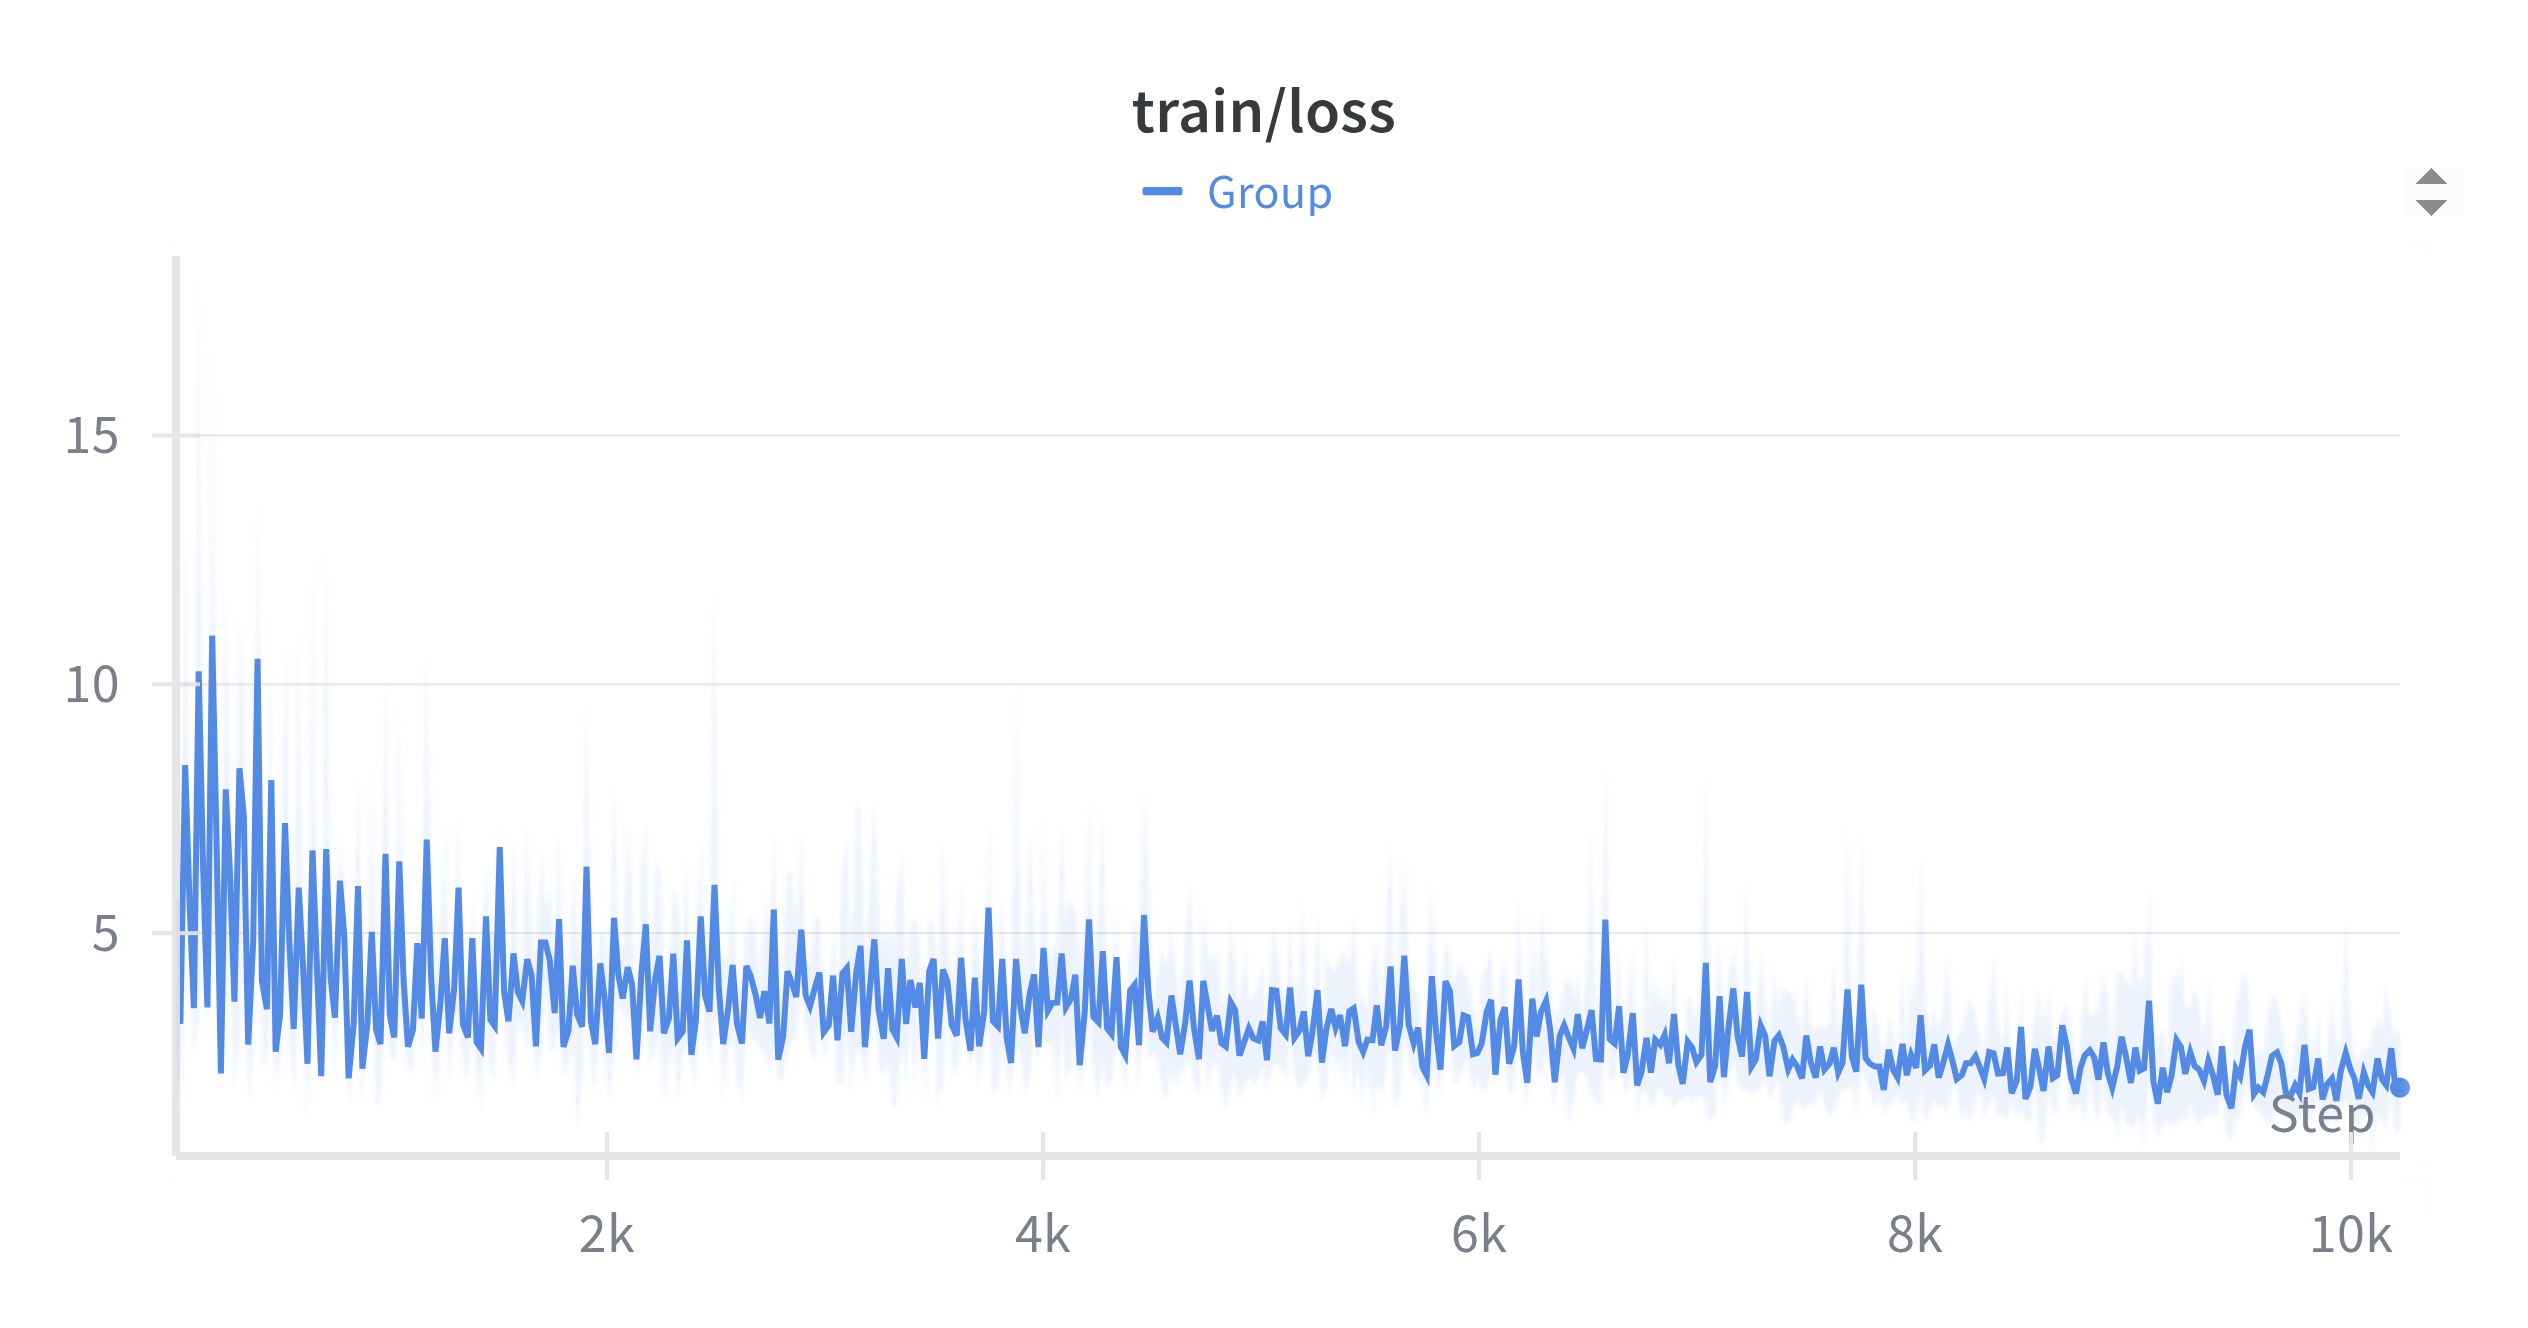
\includegraphics[width=0.7\linewidth]{photos/loss rppo - raw - 3 - norm.png}
\caption{هزینه آموزش \lr{RPPO} \lr{--} پاداش بازدهی خامِ نرمال‌شده \lr{--} محیط تک‌گانه \lr{--} دوره‌های عادی}
\label{fig:ppo-raw-1env-normal}
\end{figure}



\begin{table}[H]
\centering
\caption{نتایج \lr{RPPO} \lr{--} پاداش بازدهی خامِ نرمال‌شده \lr{--} محیط‌های برداری (۳-محیط) \lr{--} دوره‌های تصادفی}
\label{tab:rppo-raw-3env-random}
\begin{tabular}{l c}
\toprule
\lr{Metric} & \lr{Mean $\pm$ Std} \\
\midrule
\lr{Annualized Return [\%]} & \lr{25.26 $\pm$ 6.75} \\
\lr{Annualized Volatility [\%]} & \lr{19.52 $\pm$ 1.06} \\
\lr{Max Drawdown [\%]} & \lr{-24.32 $\pm$ 1.56} \\
\lr{Average Drawdown [\%]} & \lr{-5.24 $\pm$ 1.89} \\
\lr{Sharpe Ratio} & \lr{1.26 $\pm$ 0.33} \\
\lr{Sortino Ratio} & \lr{1.71 $\pm$ 0.46} \\
\lr{Calmar Ratio} & \lr{1.04 $\pm$ 0.31} \\
\lr{Max Drawdown Duration (days)} & \lr{146.00 $\pm$ 94.41} \\
\lr{Number of Trades} & \lr{75.00 $\pm$ 65.87} \\
\bottomrule
\end{tabular}
\end{table}


\begin{figure}[H]
\centering
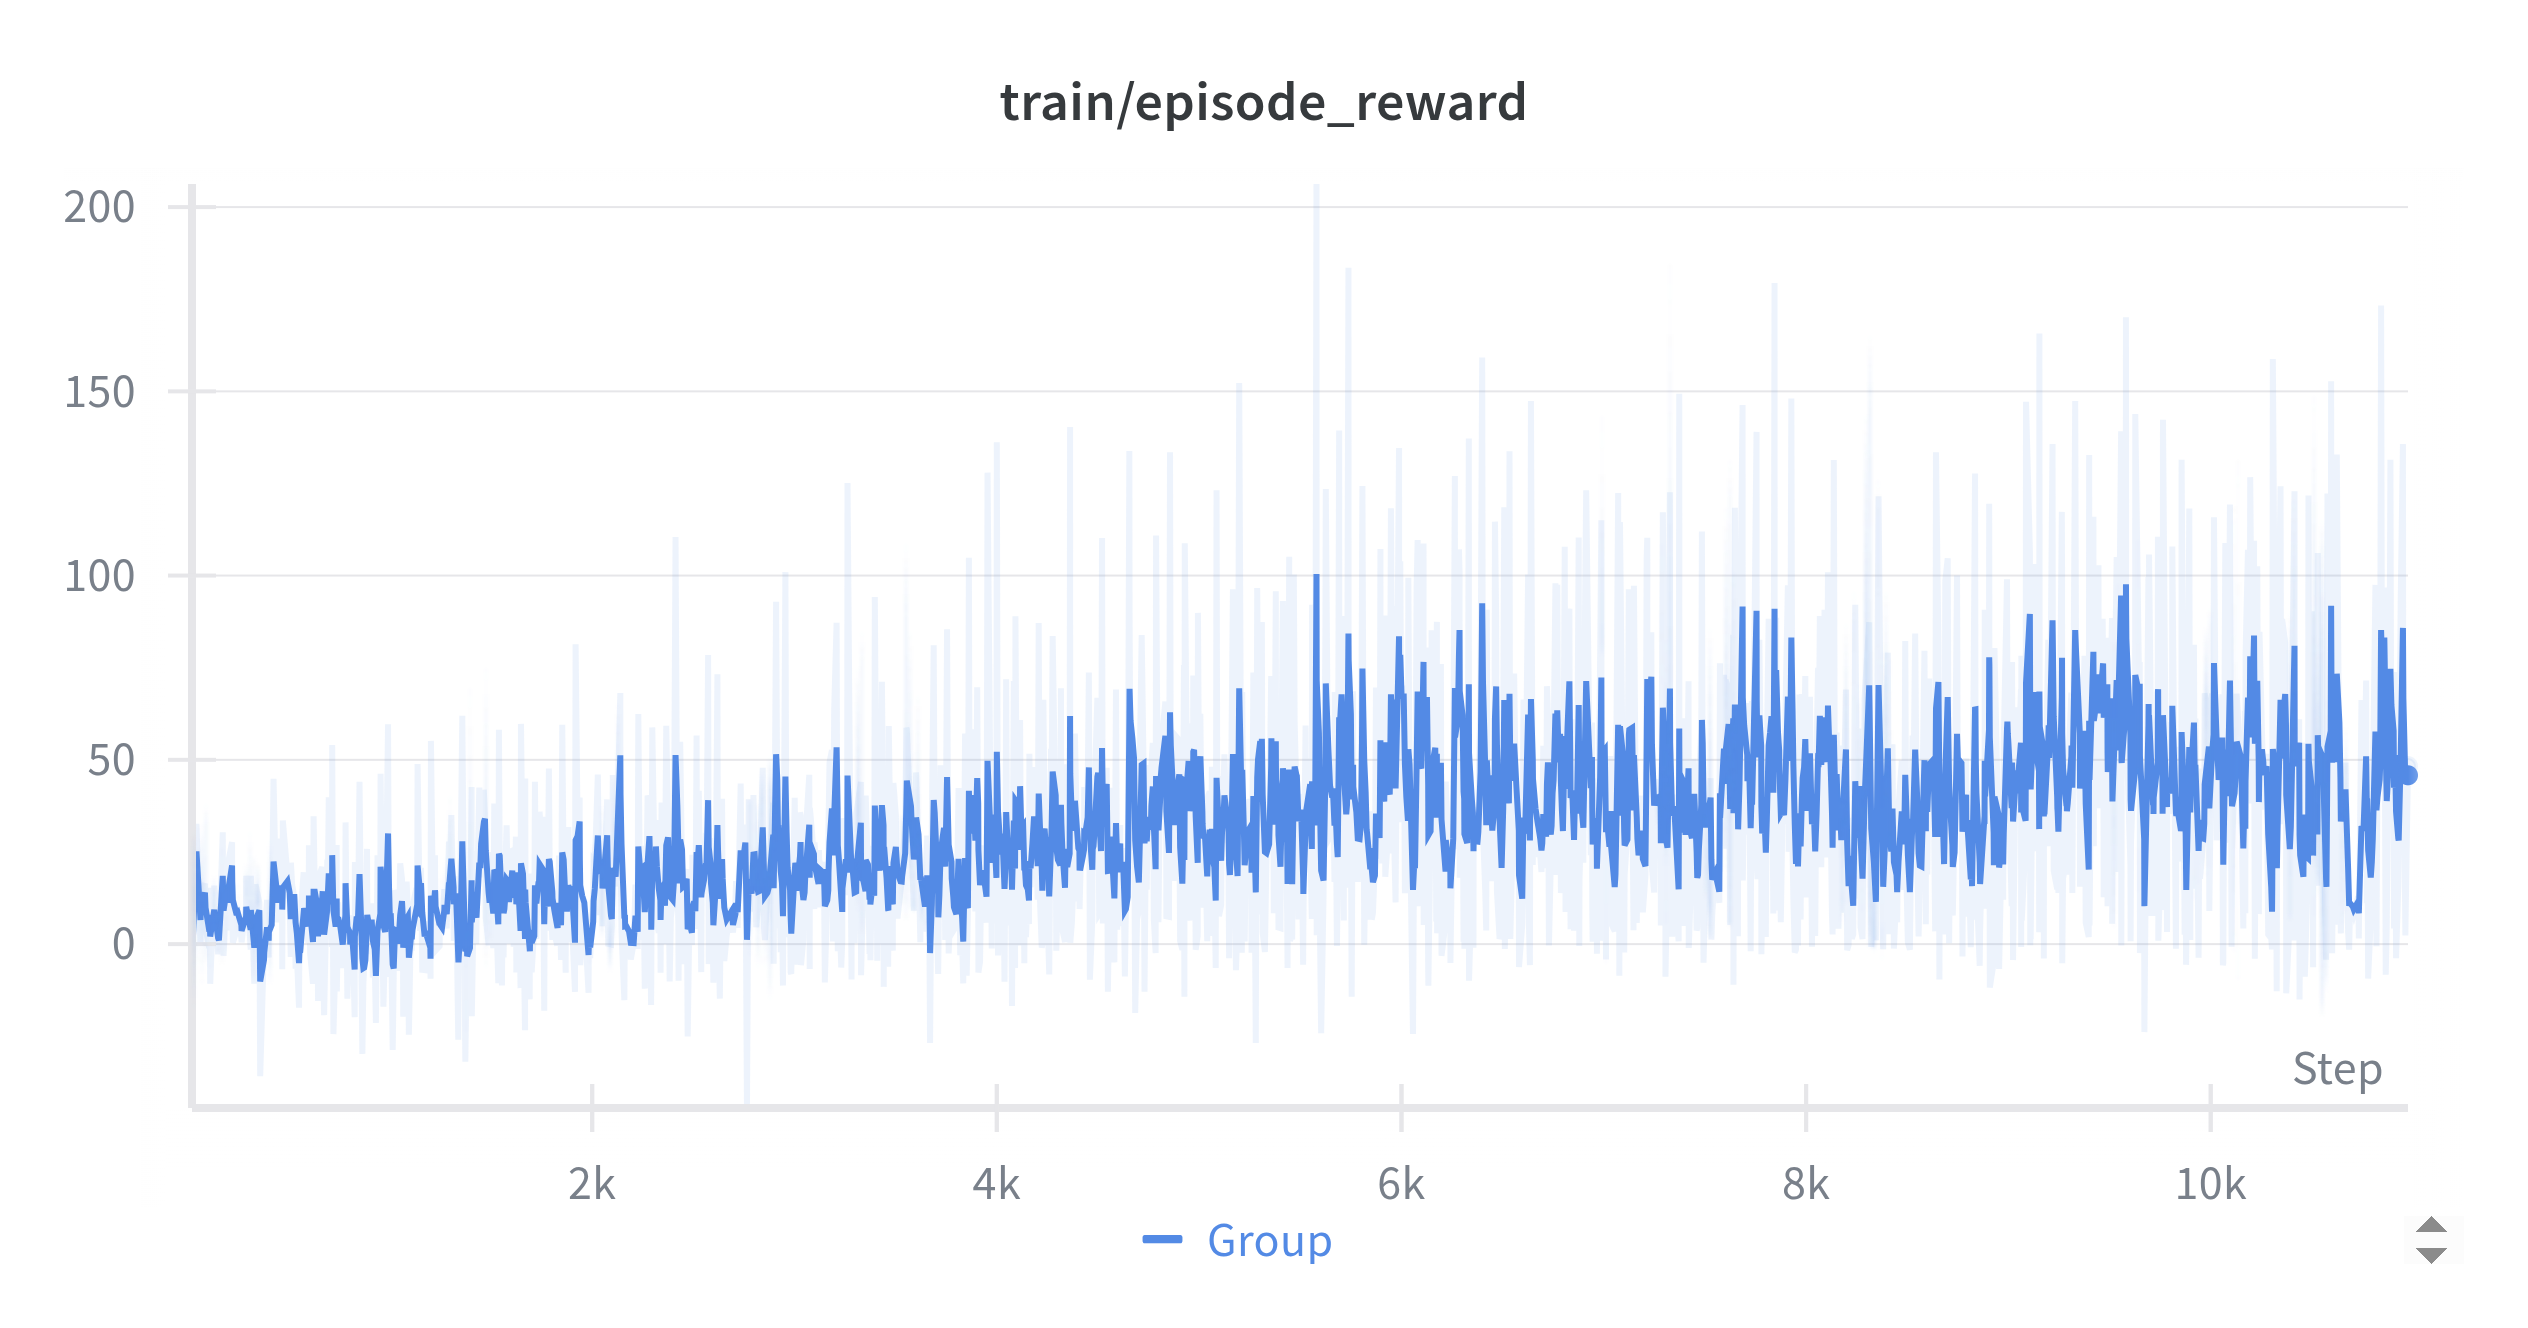
\includegraphics[width=0.7\linewidth]{photos/rew rppo - raw - 3 - rand.png}
\caption{پاداش دوره \lr{RPPO} \lr{--} پاداش بازدهی خامِ نرمال‌شده \lr{--} محیط تک‌گانه \lr{--} دوره‌های تصادفی}
\label{fig:ppo-raw-1env-normal}
\end{figure}


\begin{figure}[H]
\centering
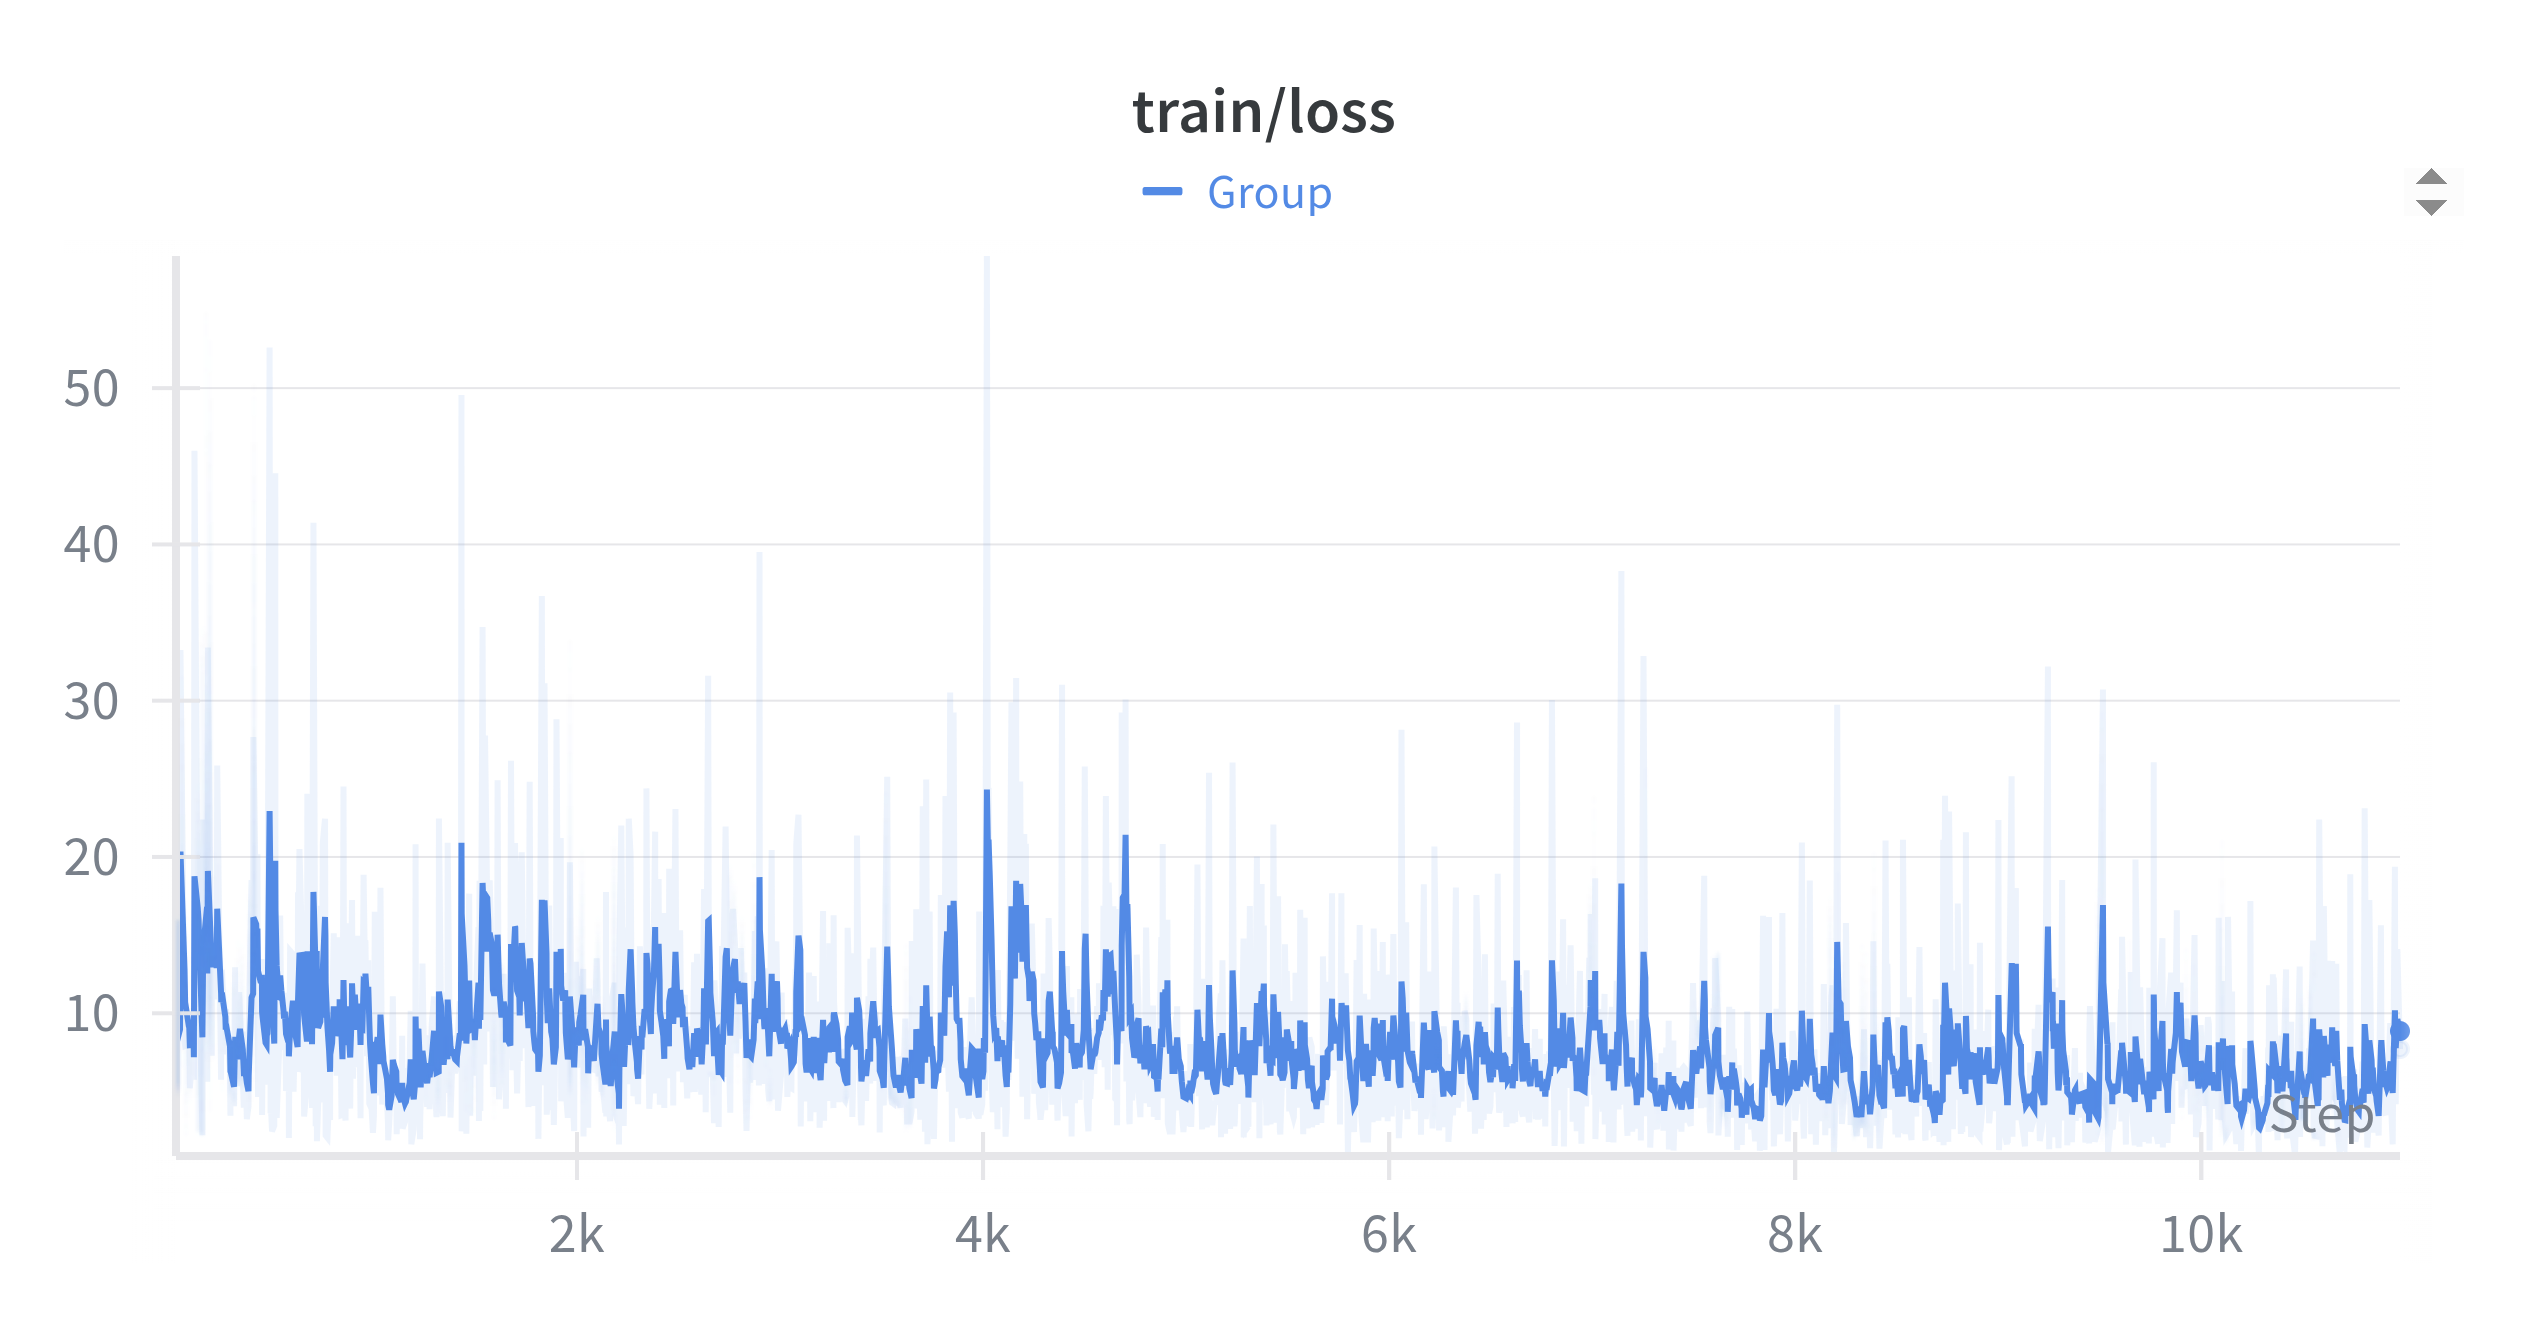
\includegraphics[width=0.7\linewidth]{photos/loss rppo - raw - 3 - rand.png}
\caption{هزینه آموزش \lr{RPPO} \lr{--} پاداش بازدهی خامِ نرمال‌شده \lr{--} محیط تک‌گانه \lr{--} دوره‌های تصادفی}
\label{fig:ppo-raw-1env-normal}
\end{figure}



\begin{table}[H]
\centering
\caption{نتایج \lr{RPPO} \lr{--} پاداش پاداش لگاریتمی تعدیل‌شده \lr{--} محیط تک‌گانه \lr{--} دوره‌های عادی}
\label{tab:rppo-logrisk-1env-normal}
\begin{tabular}{l c}
\toprule
\lr{Metric} & \lr{Mean $\pm$ Std} \\
\midrule
\lr{Annualized Return [\%]} & \lr{25.47 $\pm$ 4.32} \\
\lr{Annualized Volatility [\%]} & \lr{20.18 $\pm$ 1.94} \\
\lr{Max Drawdown [\%]} & \lr{-25.33 $\pm$ 2.01} \\
\lr{Average Drawdown [\%]} & \lr{-5.21 $\pm$ 0.72} \\
\lr{Sharpe Ratio} & \lr{1.23 $\pm$ 0.17} \\
\lr{Sortino Ratio} & \lr{1.64 $\pm$ 0.26} \\
\lr{Calmar Ratio} & \lr{1.00 $\pm$ 0.11} \\
\lr{Max Drawdown Duration (days)} & \lr{120.60 $\pm$ 24.14} \\
\lr{Number of Trades} & \lr{85.80 $\pm$ 39.42} \\
\bottomrule
\end{tabular}
\end{table}


\begin{figure}[H]
\centering
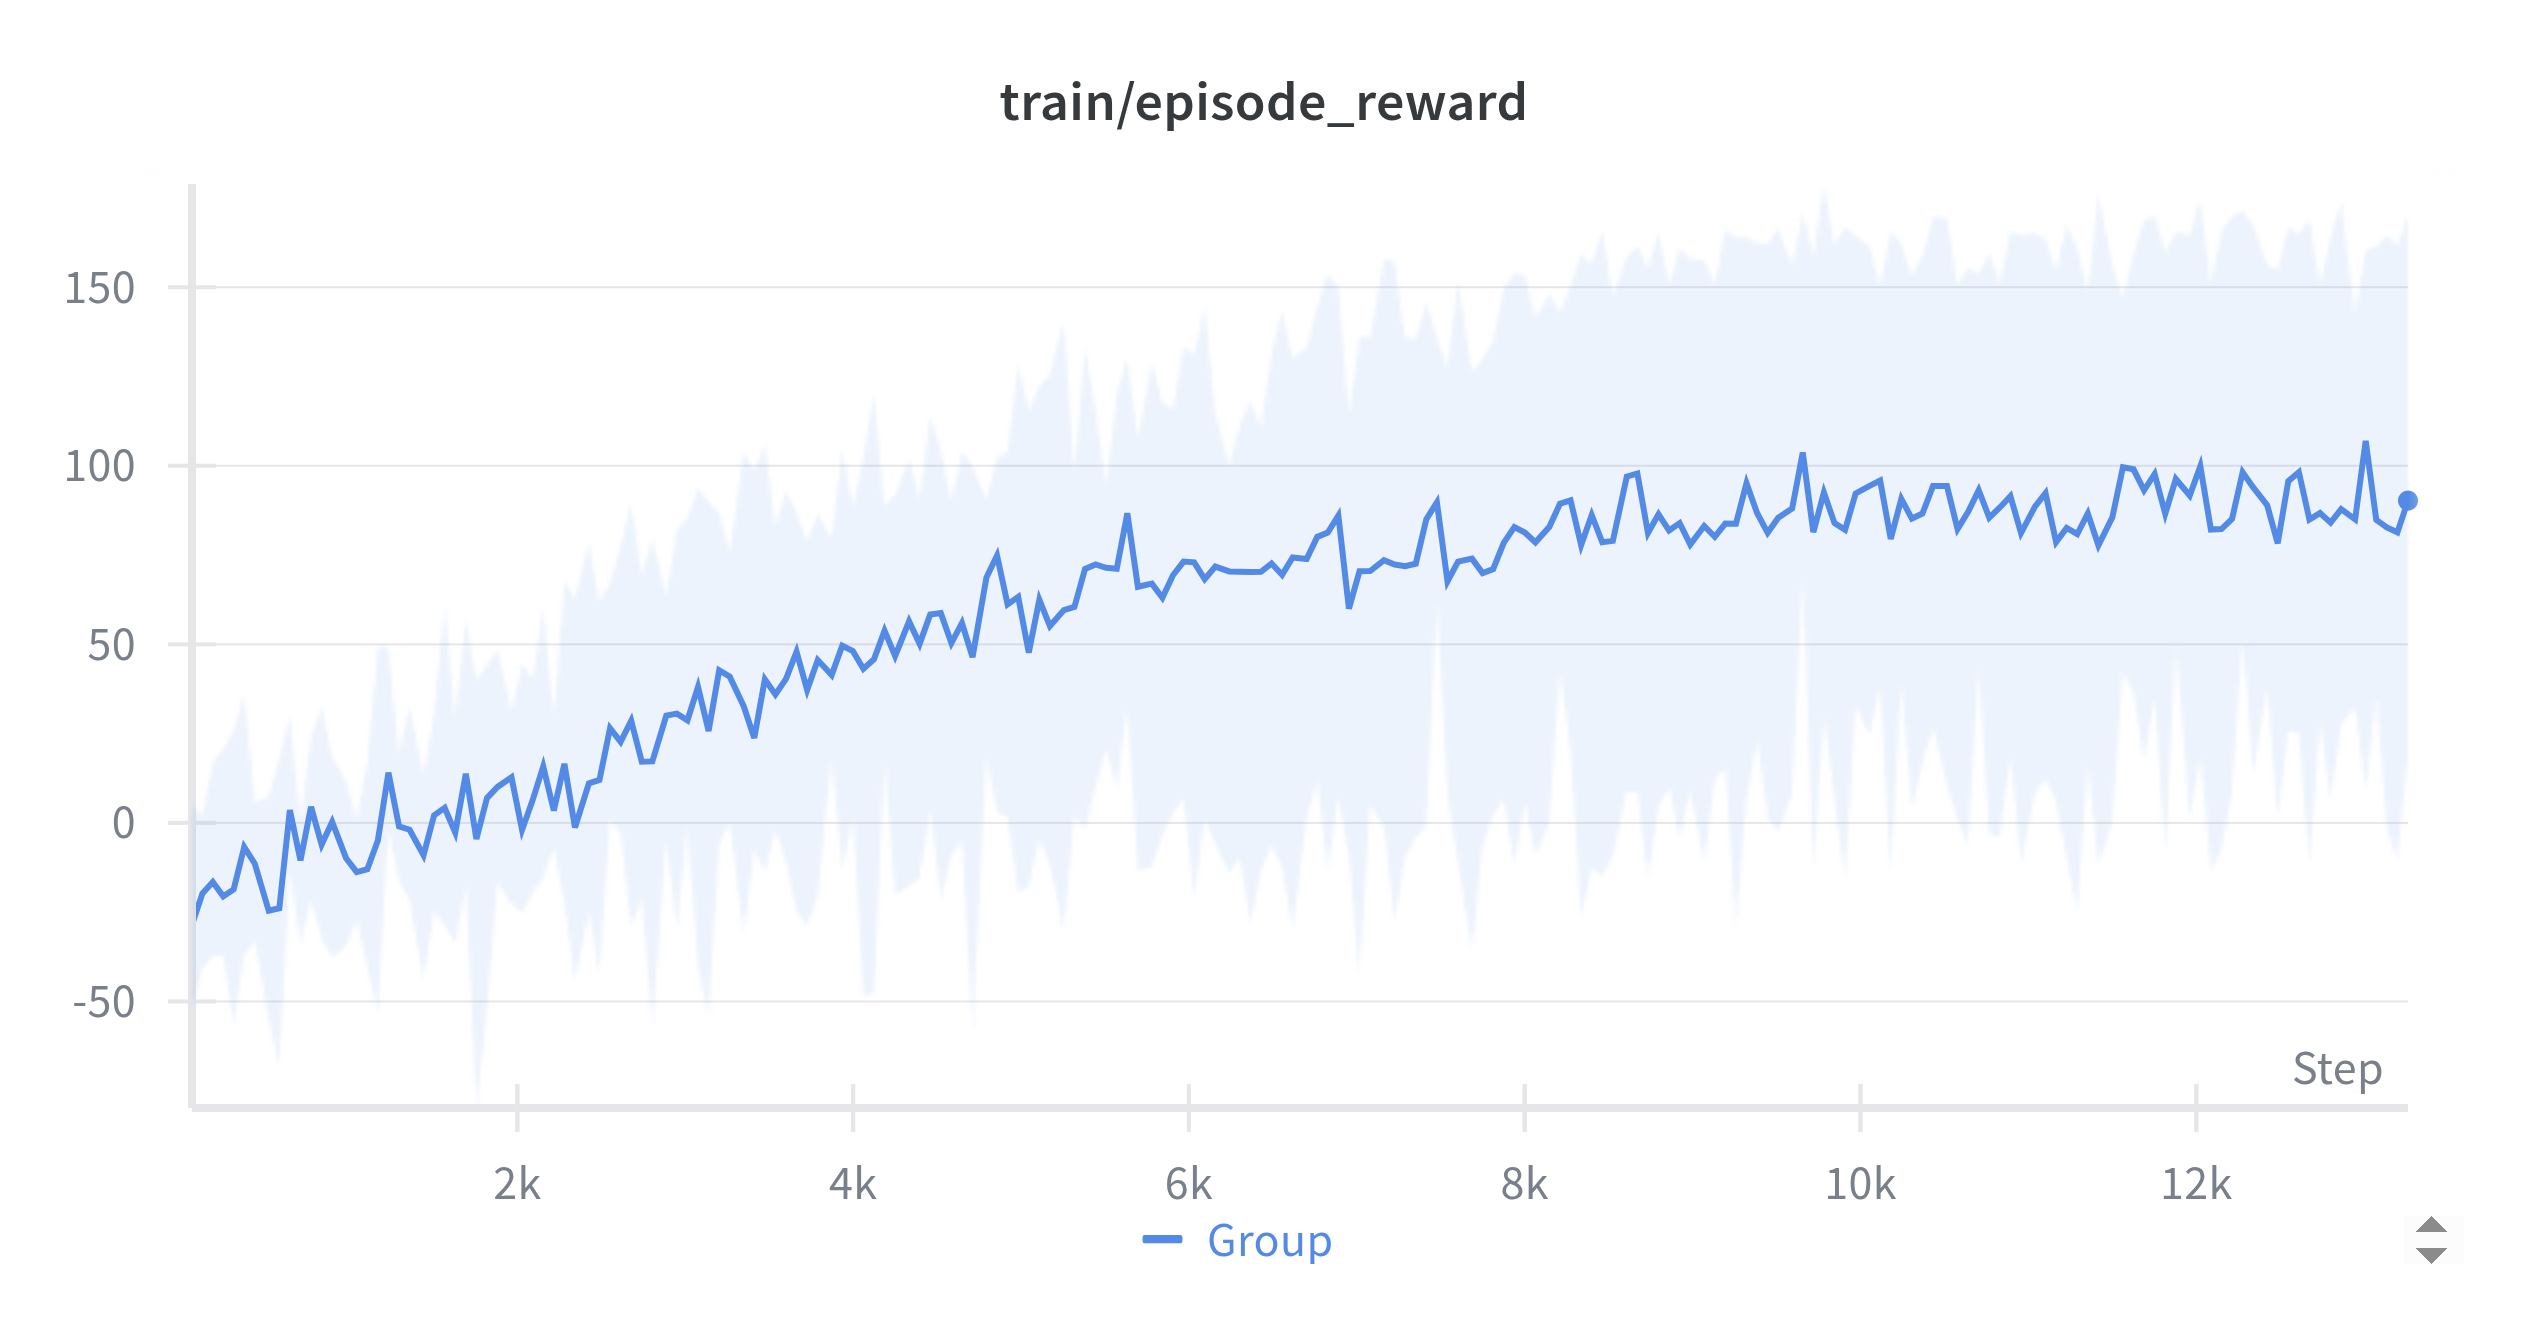
\includegraphics[width=0.7\linewidth]{photos/rew rppo - log - 1 - norm.png}
\caption{پاداش دوره \lr{RPPO} \lr{--}  پاداش لگاریتمی تعدیل‌شده \lr{--} محیط تک‌گانه \lr{--} دوره‌های تصادفی}
\label{fig:ppo-raw-1env-normal}
\end{figure}


\begin{figure}[H]
\centering
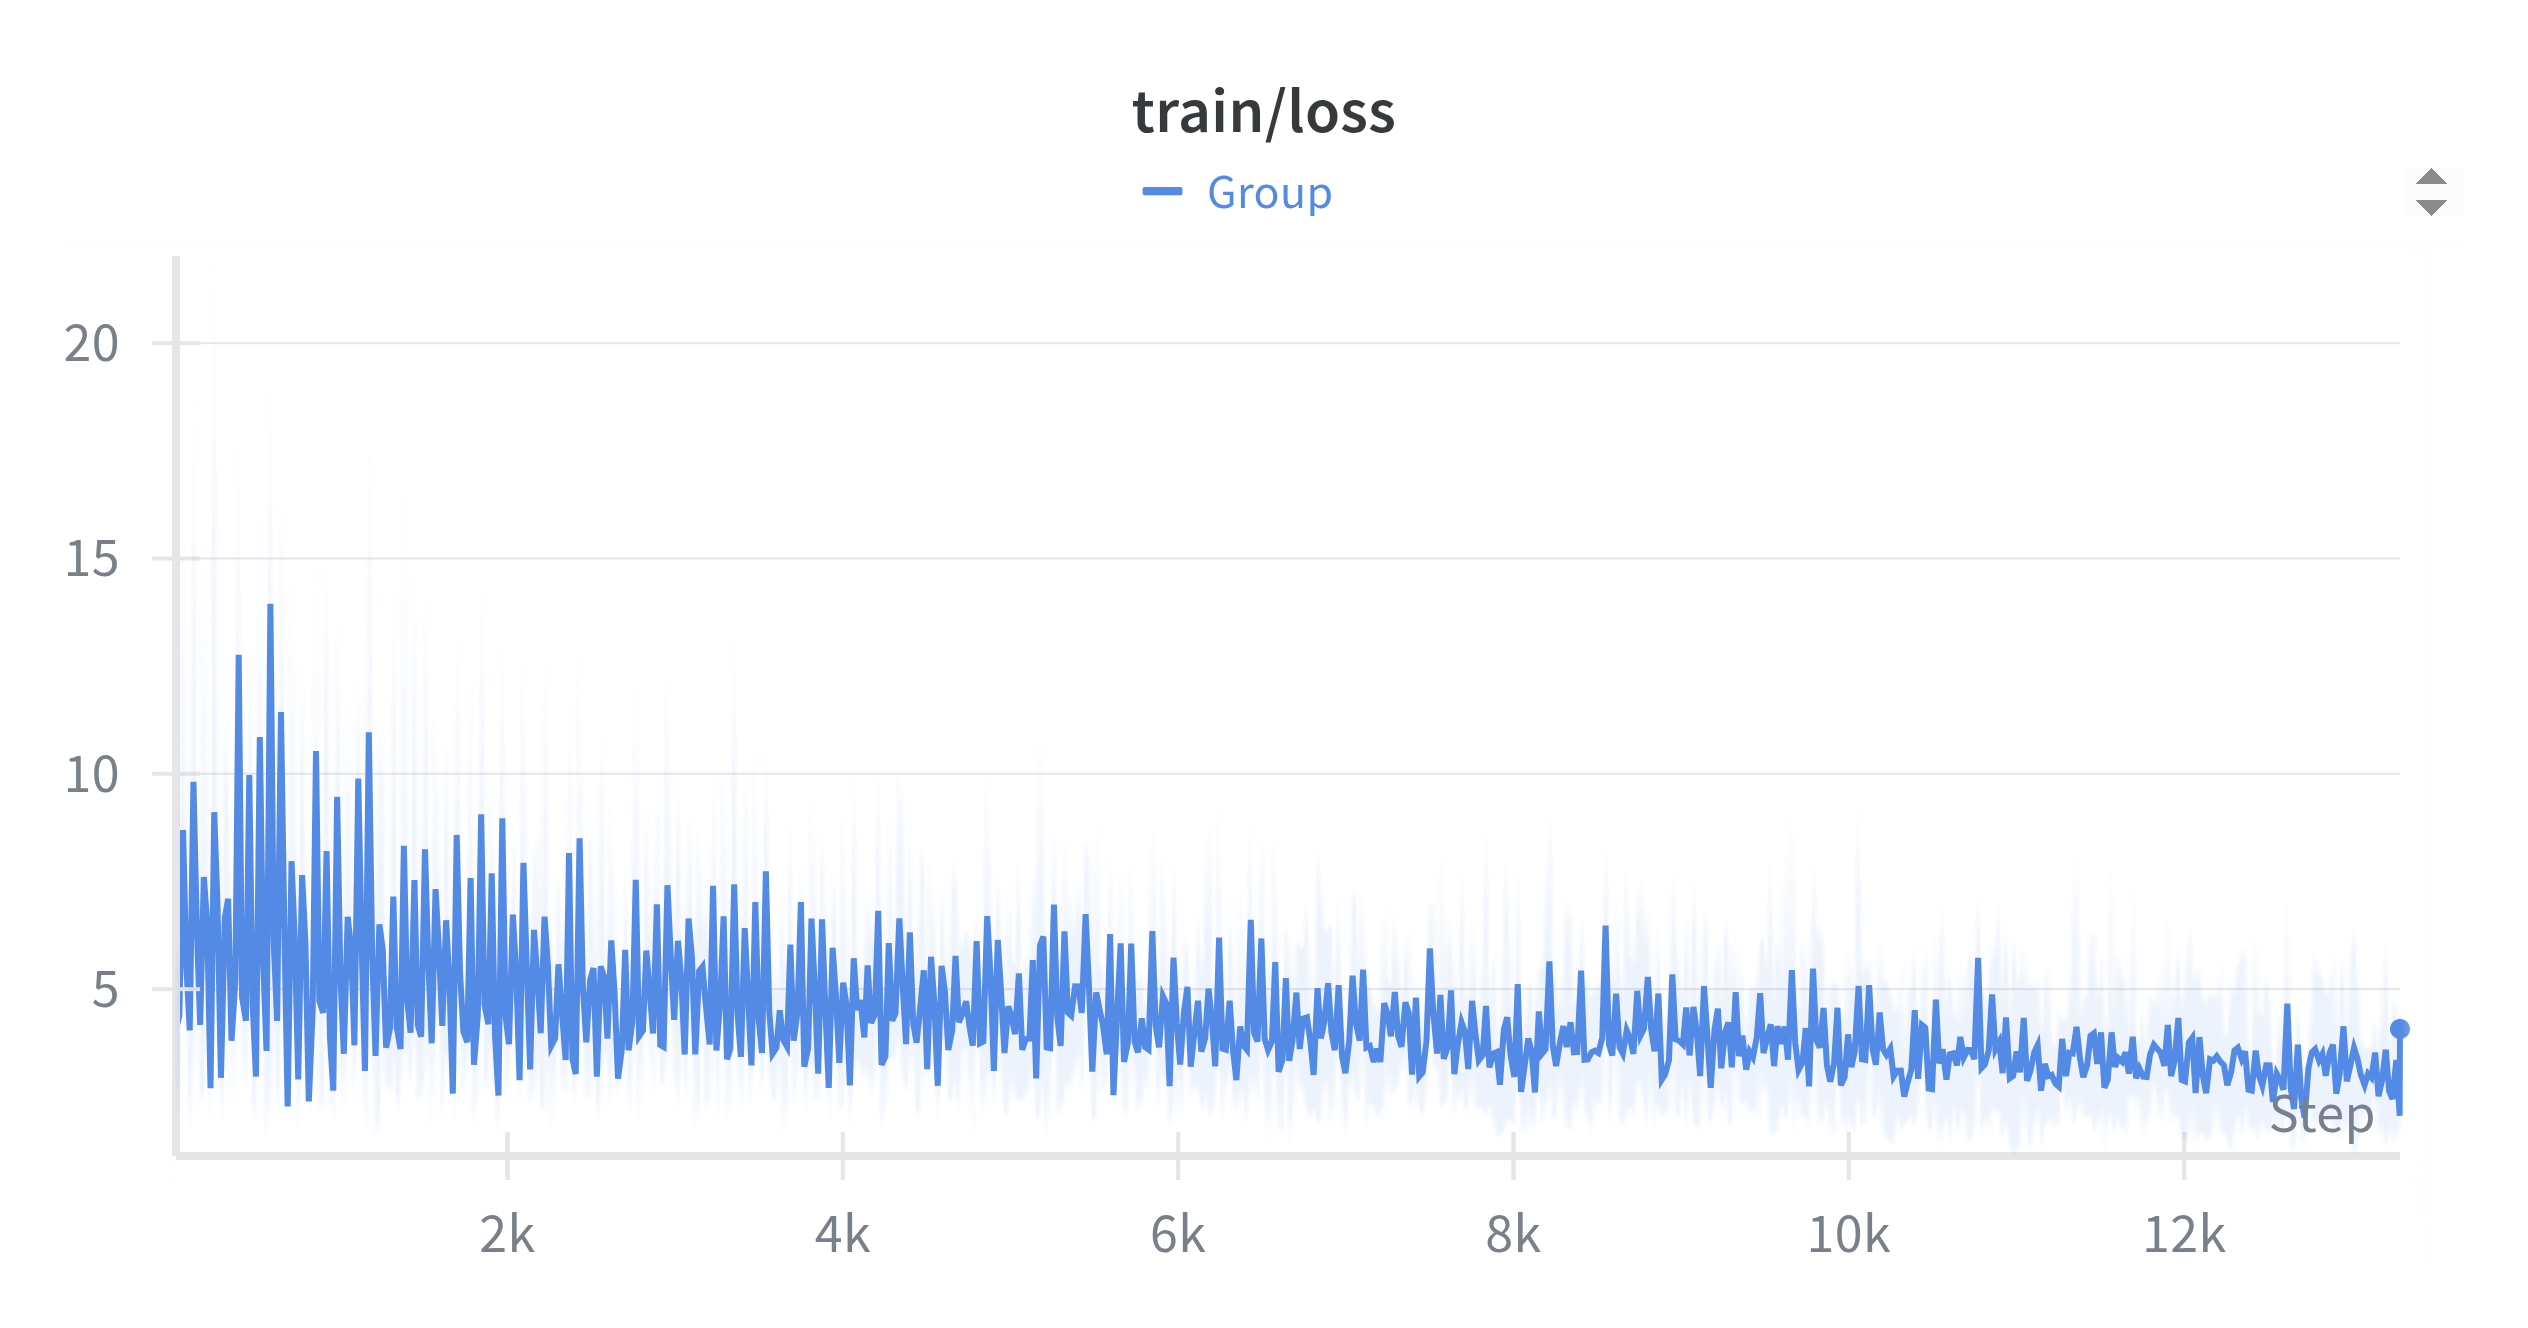
\includegraphics[width=0.7\linewidth]{photos/loss rppo - log - 1 - norm.png}
\caption{هزینه آموزش \lr{RPPO} \lr{--}  پاداش لگاریتمی تعدیل‌شده\lr{--} محیط تک‌گانه \lr{--} دوره‌های تصادفی}
\label{fig:ppo-raw-1env-normal}
\end{figure}


\begin{table}[H]
\centering
\caption{نتایج \lr{RPPO} \lr{--} پاداش لگاریتمی تعدیل‌شده \lr{--} محیط‌های برداری (۳-محیط) \lr{--} دوره‌های عادی}
\label{tab:rppo-logrisk-3env-normal}
\begin{tabular}{l c}
\toprule
\lr{Metric} & \lr{Mean $\pm$ Std} \\
\midrule
\lr{Annualized Return [\%]} & \lr{27.01 $\pm$ 3.13} \\
\lr{Annualized Volatility [\%]} & \lr{19.48 $\pm$ 1.33} \\
\lr{Max Drawdown [\%]} & \lr{-25.46 $\pm$ 2.07} \\
\lr{Average Drawdown [\%]} & \lr{-4.90 $\pm$ 0.68} \\
\lr{Sharpe Ratio} & \lr{1.33 $\pm$ 0.12} \\
\lr{Sortino Ratio} & \lr{1.79 $\pm$ 0.18} \\
\lr{Calmar Ratio} & \lr{1.06 $\pm$ 0.04} \\
\lr{Max Drawdown Duration (days)} & \lr{117.25 $\pm$ 15.95} \\
\lr{Number of Trades} & \lr{119.25 $\pm$ 31.69} \\
\bottomrule
\end{tabular}
\end{table}

\begin{figure}[H]
\centering
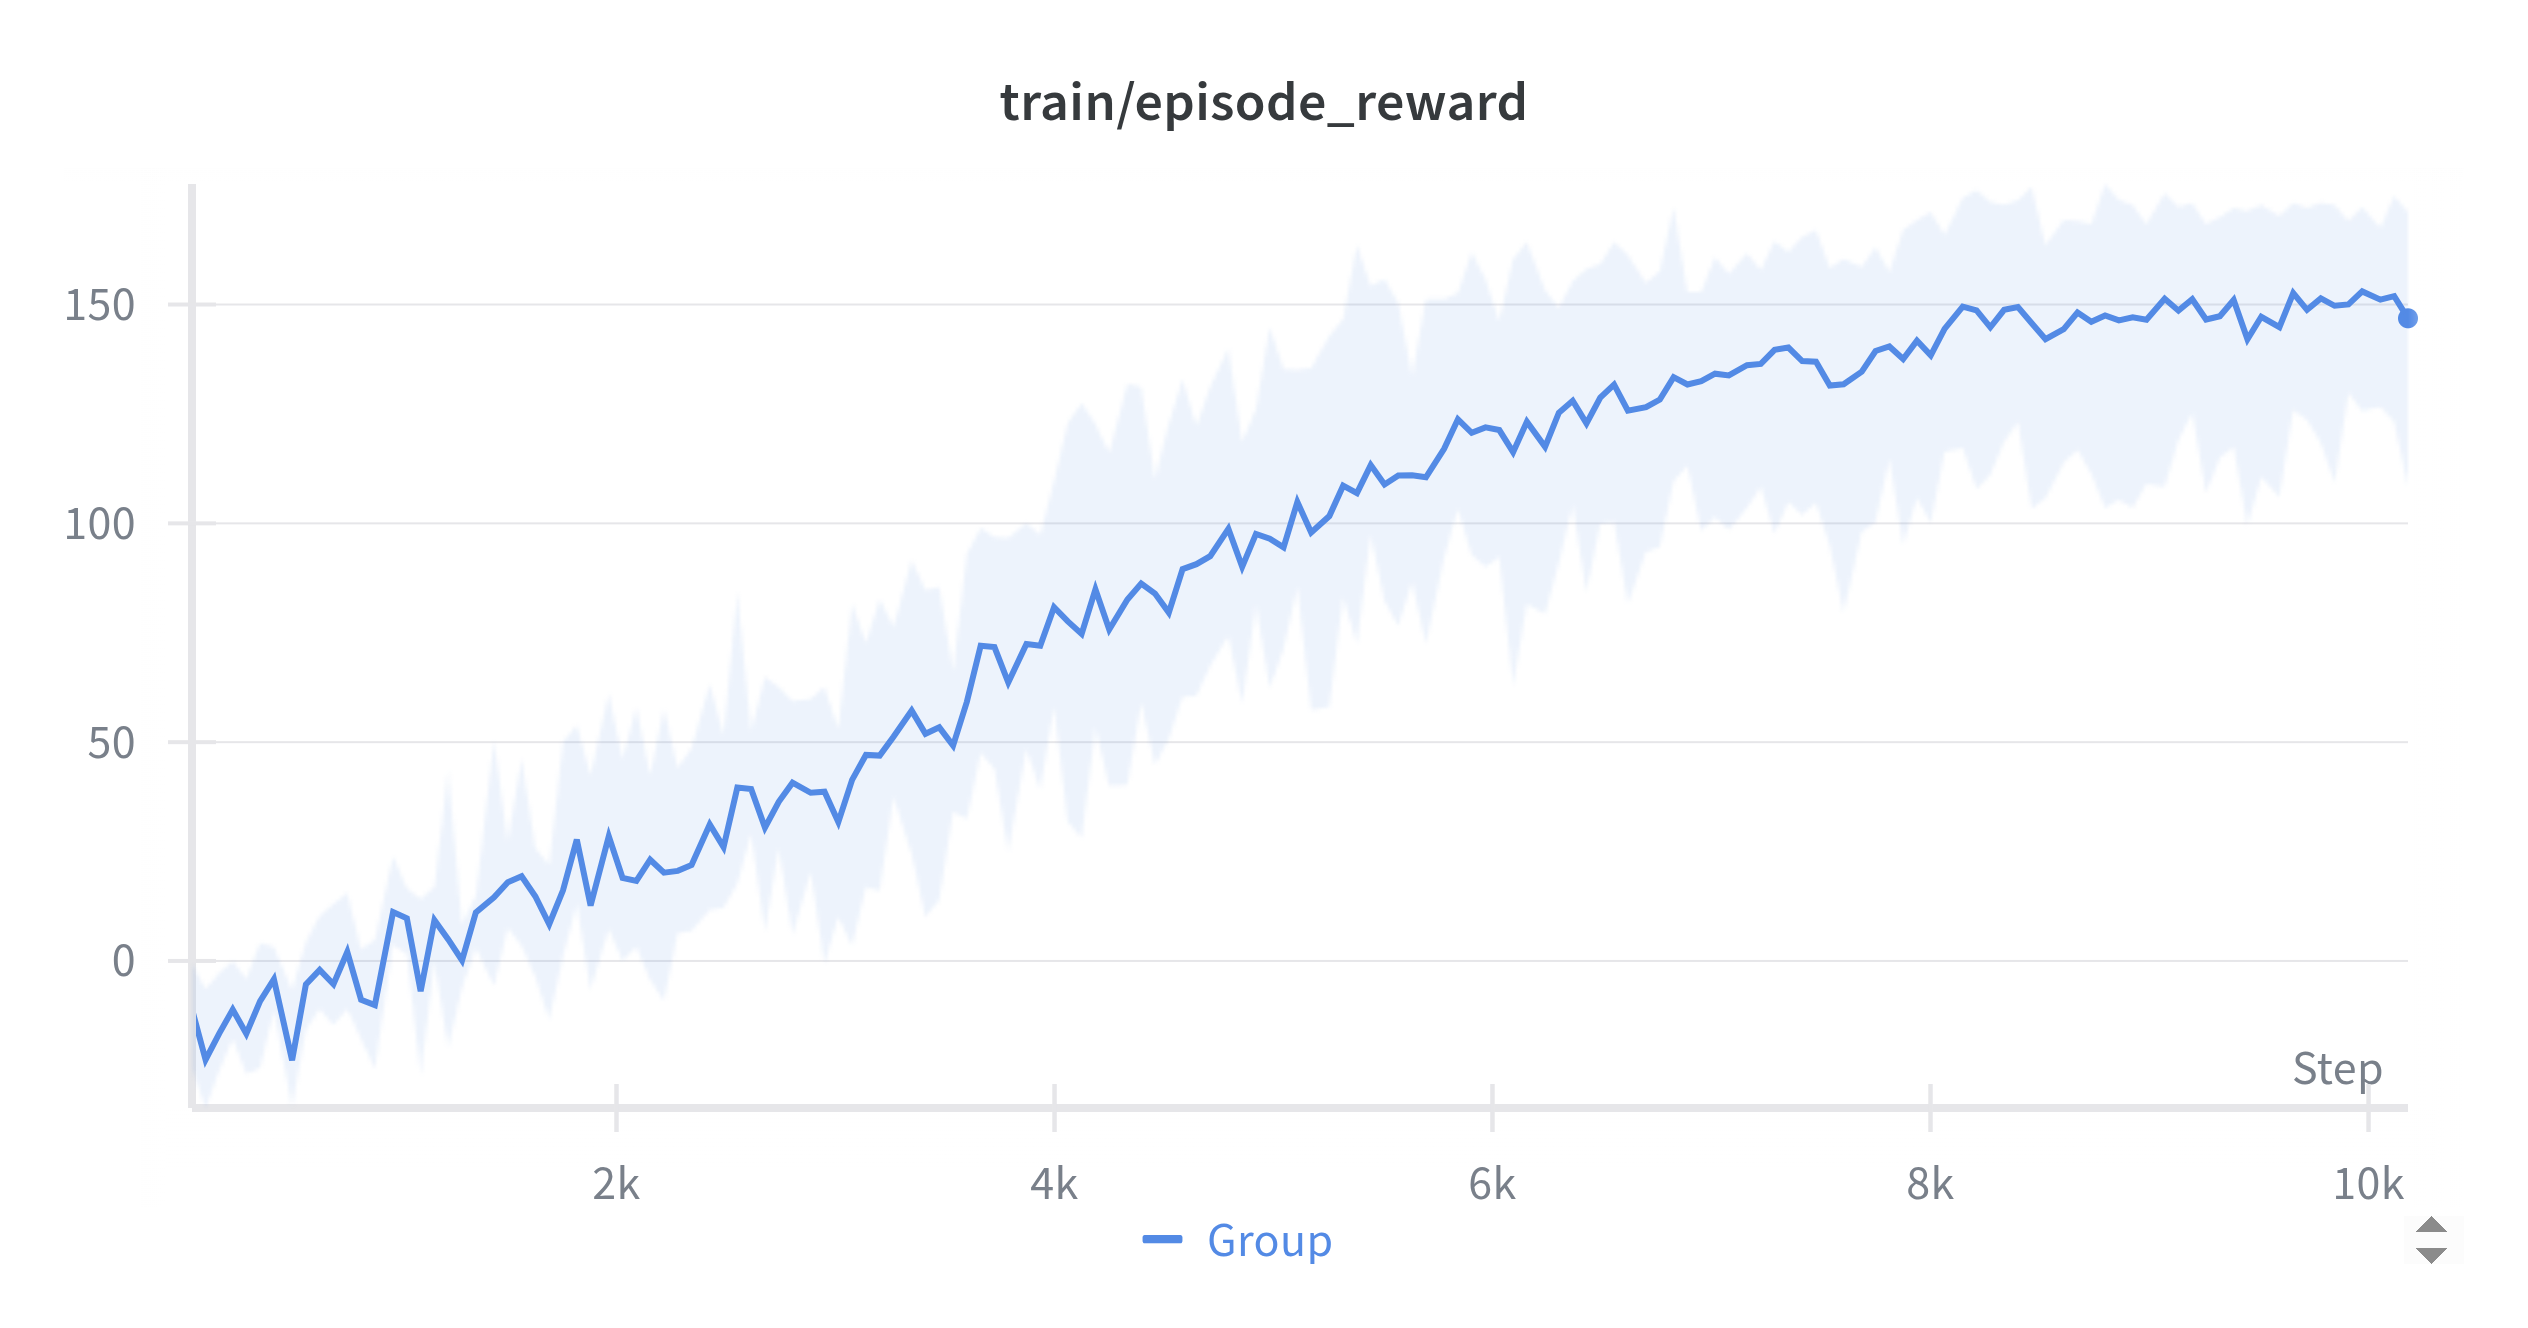
\includegraphics[width=0.7\linewidth]{photos/rew rppo - log - 3 - norm.png}
\caption{پاداش دوره \lr{RPPO} \lr{--}  پاداش لگاریتمی تعدیل‌شده \lr{--} محیط‌های برداری (۳-محیط) \lr{--} دوره‌های تصادفی}
\label{fig:ppo-raw-1env-normal}
\end{figure}


\begin{figure}[H]
\centering
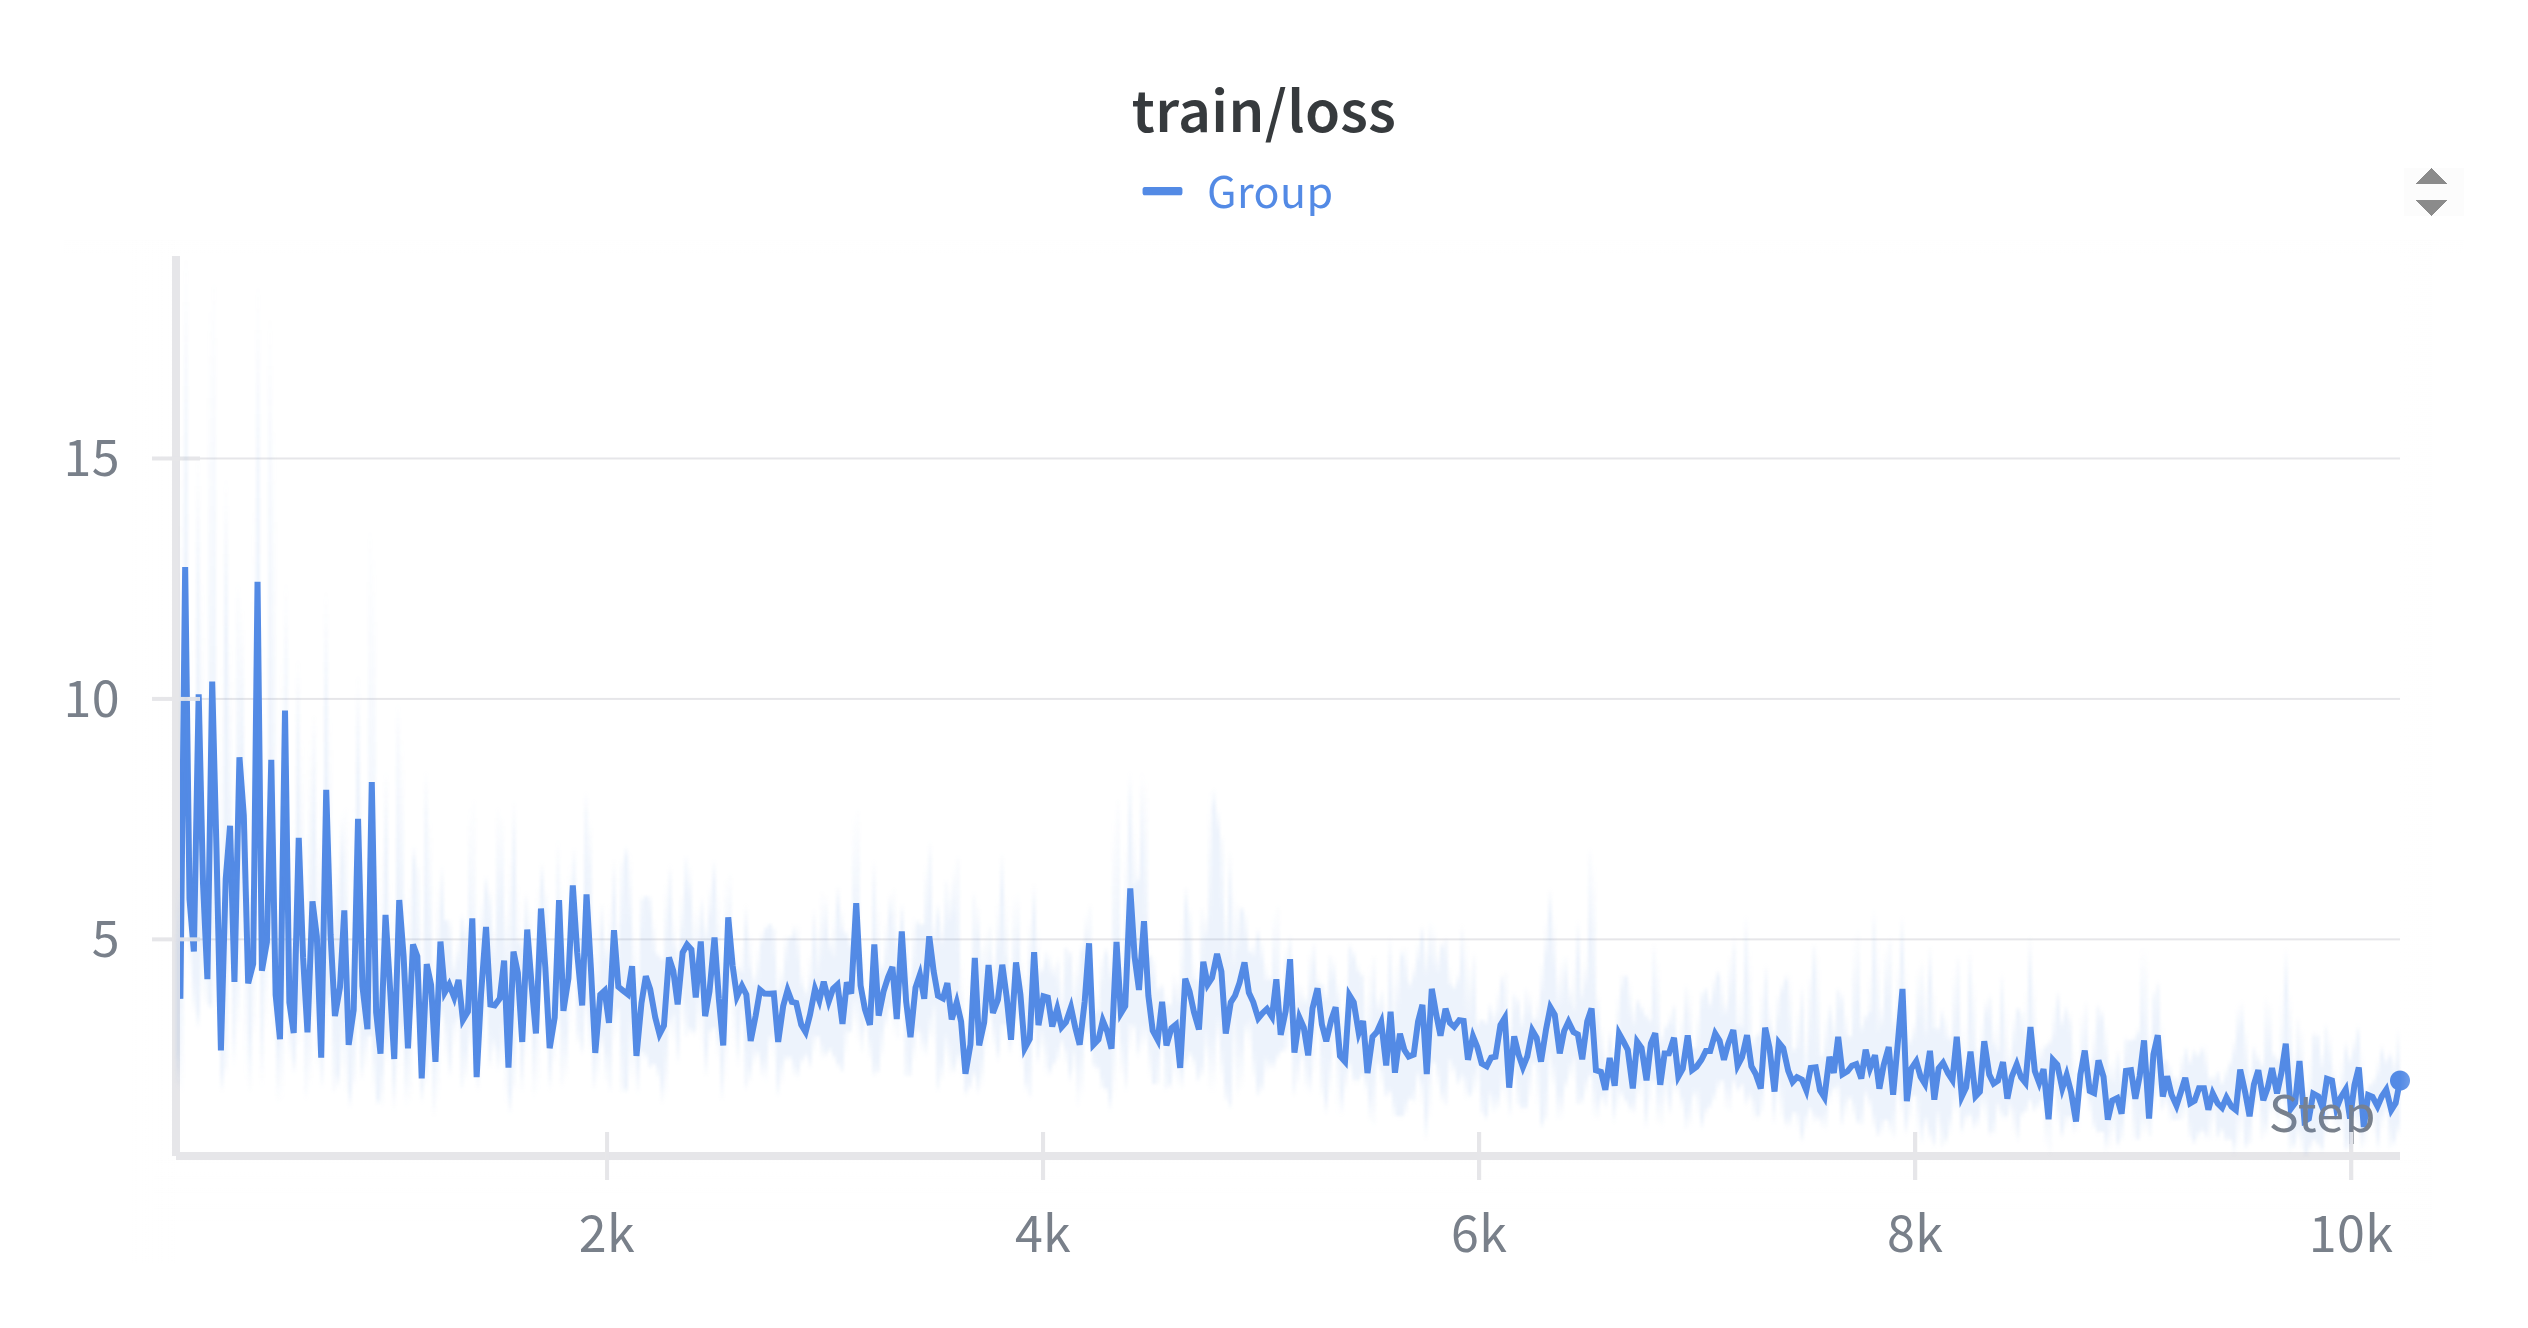
\includegraphics[width=0.7\linewidth]{photos/loss rppo - log - 3 - norm.png}
\caption{هزینه آموزش \lr{RPPO} \lr{--}  پاداش لگاریتمی تعدیل‌شده\lr{--} محیط‌های برداری (۳-محیط) \lr{--} دوره‌های تصادفی}
\label{fig:ppo-raw-1env-normal}
\end{figure}


\section{جمع‌بندی}

در این بخش، جداول مقایسه‌ای کلی از حالت‌های مختلف ارائه شدند. 
تفسیر و تحلیل عمیق‌تر نتایج به فصل هشتم (بحث و تحلیل) موکول می‌شود.

\begin{table}[H]
\centering
\caption{مقایسه کلی عملکرد \lr{PPO} و \lr{RPPO} در سناریوهای مختلف}
\label{tab:overall-comparison}
\resizebox{\textwidth}{!}{%
\begin{tabular}{lcccccc}
\toprule
\lr{Condition} & \lr{Annualized Return [\%]} & \lr{Volatility [\%]} & \lr{Sharpe} & \lr{Sortino} & \lr{Calmar} & \lr{Max Drawdown [\%]} \\
\midrule
\lr{PPO -- Raw -- 1env -- Normal}   & \lr{25.65 $\pm$ 4.47} & \lr{20.46 $\pm$ 1.07} & \lr{1.22 $\pm$ 0.19} & \lr{1.58 $\pm$ 0.24} & \lr{1.04 $\pm$ 0.19} & \lr{-24.78 $\pm$ 1.82} \\
\lr{PPO -- Raw -- 1env -- Random}   & \lr{21.35 $\pm$ 4.97} & \lr{19.25 $\pm$ 2.13} & \lr{1.11 $\pm$ 0.22} & \lr{1.48 $\pm$ 0.29} & \lr{0.91 $\pm$ 0.20} & \lr{-23.43 $\pm$ 1.94} \\
\lr{PPO -- Raw -- 3env -- Normal}   & \lr{19.10 $\pm$ 3.98} & \lr{21.25 $\pm$ 1.35} & \lr{0.93 $\pm$ 0.14} & \lr{1.24 $\pm$ 0.18} & \lr{0.79 $\pm$ 0.18} & \lr{-24.33 $\pm$ 2.20} \\
\lr{PPO -- Raw -- 3env -- Random}   & \lr{20.89 $\pm$ 4.75} & \lr{19.21 $\pm$ 2.86} & \lr{1.09 $\pm$ 0.16} & \lr{1.45 $\pm$ 0.20} & \lr{0.90 $\pm$ 0.15} & \lr{-23.24 $\pm$ 2.86} \\
\lr{PPO -- Log -- 1env -- Normal}   & \lr{24.38 $\pm$ 8.64} & \lr{20.52 $\pm$ 1.45} & \lr{1.16 $\pm$ 0.35} & \lr{1.55 $\pm$ 0.47} & \lr{0.97 $\pm$ 0.33} & \lr{-25.03 $\pm$ 0.82} \\
\lr{PPO -- Log -- 3env -- Normal}   & \lr{21.97 $\pm$ 8.12} & \lr{20.84 $\pm$ 1.39} & \lr{1.05 $\pm$ 0.31} & \lr{1.40 $\pm$ 0.40} & \lr{0.86 $\pm$ 0.30} & \lr{-25.33 $\pm$ 0.92} \\
\lr{RPPO -- Raw -- 1env -- Normal}  & \lr{22.67 $\pm$ 5.21} & \lr{19.68 $\pm$ 1.73} & \lr{1.14 $\pm$ 0.23} & \lr{1.53 $\pm$ 0.31} & \lr{0.93 $\pm$ 0.21} & \lr{-24.53 $\pm$ 1.58} \\
\lr{RPPO -- Raw -- 1env -- Random}  & \lr{22.05 $\pm$ 3.40} & \lr{19.05 $\pm$ 1.94} & \lr{1.16 $\pm$ 0.20} & \lr{1.56 $\pm$ 0.26} & \lr{0.92 $\pm$ 0.16} & \lr{-24.13 $\pm$ 1.45} \\
\lr{RPPO -- Raw -- 3env -- Normal}  & \textbf{\lr{28.62 $\pm$ 2.23}} & \lr{19.60 $\pm$ 1.69} & \textbf{\lr{1.39 $\pm$ 0.04}} & \textbf{\lr{1.83 $\pm$ 0.11}} & \textbf{\lr{1.14 $\pm$ 0.06}} & \lr{-25.11 $\pm$ 2.97} \\
\lr{RPPO -- Raw -- 3env -- Random}  & \lr{25.26 $\pm$ 6.75} & \lr{19.52 $\pm$ 1.06} & \lr{1.26 $\pm$ 0.33} & \lr{1.71 $\pm$ 0.46} & \lr{1.04 $\pm$ 0.31} & \lr{-24.32 $\pm$ 1.56} \\
\lr{RPPO -- Log -- 1env -- Normal}  & \lr{25.47 $\pm$ 4.32} & \lr{20.18 $\pm$ 1.94} & \lr{1.23 $\pm$ 0.17} & \lr{1.64 $\pm$ 0.26} & \lr{1.00 $\pm$ 0.11} & \lr{-25.33 $\pm$ 2.01} \\
\lr{RPPO -- Log -- 3env -- Normal}  & \lr{27.01 $\pm$ 3.13} & \textbf{\lr{19.48 $\pm$ 1.33}} & \lr{1.33 $\pm$ 0.12} & \lr{1.79 $\pm$ 0.18} & \lr{1.06 $\pm$ 0.04} & \textbf{\lr{-24.90 $\pm$ 2.07}} \\
\bottomrule
\end{tabular}%
}
\end{table}

\begin{table}[H]
\centering
\caption{مقایسه میانگین عملکرد \lr{PPO} و \lr{RPPO}}
\label{tab:avg-ppo-vs-rppo}
\resizebox{\textwidth}{!}{%
\begin{tabular}{lcccccc}
\toprule
\lr{Algorithm} & \lr{Annualized Return [\%]} & \lr{Volatility [\%]} & \lr{Sharpe} & \lr{Sortino} & \lr{Calmar} & \lr{Max Drawdown [\%]} \\
\midrule
\lr{PPO (avg)}  & \lr{22.22 $\pm$ 2.39} & \lr{20.26 $\pm$ 0.57} & \lr{1.09 $\pm$ 0.10} & \lr{1.45 $\pm$ 0.12} & \lr{0.91 $\pm$ 0.09} & \textbf{\lr{-24.36 $\pm$ 0.80}} \\
\lr{RPPO (avg)} & \textbf{\lr{25.18 $\pm$ 2.33}} & \textbf{\lr{19.58 $\pm$ 0.28}} & \textbf{\lr{1.25 $\pm$ 0.09}} & \textbf{\lr{1.68 $\pm$ 0.13}} & \textbf{\lr{1.01 $\pm$ 0.08}} & \lr{-24.81 $\pm$ 0.44} \\
\bottomrule
\end{tabular}
}
\end{table}

\begin{table}[H]
\centering
\caption{مقایسه میانگین عملکرد \lr{Raw} در برابر پاداش لگاریتمی تعدیل‌شده}
\label{tab:avg-raw-vs-log}
\resizebox{\textwidth}{!}{%
\begin{tabular}{lcccccc}
\toprule
\lr{Reward Type} & \lr{Annualized Return [\%]} & \lr{Volatility [\%]} & \lr{Sharpe} & \lr{Sortino} & \lr{Calmar} & \lr{Max Drawdown [\%]} \\
\midrule
\lr{Raw (avg)} & \lr{23.20 $\pm$ 3.08} & \textbf{\lr{19.75 $\pm$ 0.82}} & \lr{1.16 $\pm$ 0.15} & \lr{1.55 $\pm$ 0.17} & \lr{0.96 $\pm$ 0.11} & \textbf{\lr{-24.23 $\pm$ 0.56}} \\
\lr{Log (avg)} & \textbf{\lr{24.71 $\pm$ 2.12}} & \lr{20.26 $\pm$ 0.29} & \textbf{\lr{1.19 $\pm$ 0.09}} & \textbf{\lr{1.60 $\pm$ 0.12}} & \textbf{\lr{0.97 $\pm$ 0.06}} & \lr{-25.29 $\pm$ 0.14} \\
\bottomrule
\end{tabular}
}
\end{table}

\begin{table}[H]
\centering
\caption{مقایسه میانگین عملکرد محیط تک‌گانه در برابر محیط‌های برداری (۳-محیط)}
\label{tab:avg-1env-vs-3env}
\resizebox{\textwidth}{!}{%
\begin{tabular}{lcccccc}
\toprule
\lr{Env} & \lr{Annualized Return [\%]} & \lr{Volatility [\%]} & \lr{Sharpe} & \lr{Sortino} & \lr{Calmar} & \lr{Max Drawdown [\%]} \\
\midrule
\lr{1env (avg)} & \lr{23.60 $\pm$ 1.77} & \textbf{\lr{19.86 $\pm$ 0.62}} & \lr{1.17 $\pm$ 0.07} & \lr{1.56 $\pm$ 0.10} & \lr{0.96 $\pm$ 0.06} & \textbf{\lr{-24.54 $\pm$ 0.42}} \\
\lr{3env (avg)} & \textbf{\lr{23.81 $\pm$ 2.74}} & \lr{19.98 $\pm$ 0.90} & \textbf{\lr{1.18 $\pm$ 0.13}} & \textbf{\lr{1.57 $\pm$ 0.16}} & \lr{0.96 $\pm$ 0.12} & \lr{-24.63 $\pm$ 0.79} \\
\bottomrule
\end{tabular}
}
\end{table}

\begin{table}[H]
\centering
\caption{مقایسه میانگین عملکرد دوره‌های عادی در برابر دوره‌های تصادفی}
\label{tab:avg-normal-vs-random}
\resizebox{\textwidth}{!}{%
\begin{tabular}{lcccccc}
\toprule
\lr{Regime} & \lr{Annualized Return [\%]} & \lr{Volatility [\%]} & \lr{Sharpe} & \lr{Sortino} & \lr{Calmar} & \lr{Max Drawdown [\%]} \\
\midrule
\lr{Normal (avg)} & \textbf{\lr{24.36 $\pm$ 2.94}} & \lr{20.25 $\pm$ 0.57} & \textbf{\lr{1.18 $\pm$ 0.13}} & \textbf{\lr{1.57 $\pm$ 0.16}} & \textbf{\lr{0.97 $\pm$ 0.09}} & \lr{-24.99 $\pm$ 0.44} \\
\lr{Random (avg)} & \lr{22.39 $\pm$ 1.77} & \textbf{\lr{19.26 $\pm$ 0.21}} & \lr{1.16 $\pm$ 0.07} & \lr{1.55 $\pm$ 0.10} & \lr{0.94 $\pm$ 0.06} & \textbf{\lr{-23.78 $\pm$ 0.41}} \\
\bottomrule
\end{tabular}
}
\end{table}



\chapter{بحث و تحلیل}

\section{مقدمه}

\section{تحلیل نقش منبع احساسات}

نتایج آزمون‌های \lr{Granger Causality} نشان می‌دهد که اثر سیگنال‌های احساسی بسته به نوع سهام و منبع استخراج احساسات متفاوت است. 
به‌طور کلی، \lr{FinGPT} در مقایسه با \lr{FinBERT} عملکرد قوی‌تری داشته است؛ برای نمونه، در سهام \lr{AAPL} و به‌ویژه \lr{BA} توان پیش‌بینی \lr{FinGPT} به‌مراتب بهتر بوده و در حالی‌که \lr{FinBERT} عملکرد ضعیفی داشته، \lr{FinGPT} توانسته است نتایج معناداری ارائه دهد. 
در سهام \lr{JPM} عملکرد هر دو مدل تقریباً مشابه بوده و تفاوت معناداری مشاهده نشده است. 
در مقابل، در سهام \lr{GS} که از نظر حجم و کیفیت پوشش خبری ضعیف‌تر است، هر دو مدل عملکرد پایینی داشته‌اند و حتی \lr{FinGPT} نیز نتوانسته بهبود چشمگیری ایجاد کند. 

همچنین نتایج ترکیب ویژگی‌های دو مدل نشان می‌دهد که در اغلب موارد، استفاده از ترکیب \lr{FinBERT} و \lr{FinGPT} قدرت توضیحی بیشتری ایجاد می‌کند و توانسته است در مقایسه با هر یک از مدل‌ها به‌تنهایی، روابط معنادارتری را آشکار سازد. تنها در مورد سهام \lr{BA} این ترکیب نسبت به \lr{FinGPT} بهبود محسوسی نداشته است. 

در مجموع می‌توان گفت:  
\begin{itemize}
    \item سیگنال‌های احساسی در سهام مختلف اثر یکسانی ندارند و کیفیت و حجم داده‌های خبری نقش کلیدی ایفا می‌کند.  
    \item \lr{FinGPT} معمولاً کارآمدتر از \lr{FinBERT} است، به‌ویژه در سهامی با پوشش خبری گسترده مانند \lr{AAPL} یا در مواردی که \lr{FinBERT} ضعیف عمل می‌کند (مانند \lr{BA}).  
    \item ترکیب منابع مختلف احساس به‌طور معمول نتایج بهتری به همراه دارد و نشان می‌دهد که عامل‌های یادگیری تقویتی بهتر است به جای تکیه بر یک منبع منفرد، از چندین منبع احساسات به صورت هم‌زمان استفاده کنند.  
\end{itemize}


\section{مقایسه با مدل‌های سنتی}

پیش از تحلیل نتایج، به‌طور خلاصه روش‌های سنتی مورد استفاده به‌عنوان خط مبنا معرفی می‌شوند:  
\begin{itemize}
    \item \lr{Buy \& Hold (BH)}: خرید و نگهداری دارایی در کل بازه بدون تغییر سبد سهام.  
    \item \lr{Equal-Weight (EW)}: تخصیص مساوی سرمایه به تمام دارایی‌ها، بدون توجه به ریسک یا بازده تاریخی.  
    \item \lr{DIJA}: شاخص \lr{Dow Jones Industrial Average} به‌عنوان نماینده‌ای از عملکرد کلی بازار.  
    \item \lr{Mean-Variance Optimization (MVO)}: بهینه‌سازی سبد سهام بر اساس میانگین و واریانس بازده تاریخی برای بیشینه‌سازی نسبت بازده به ریسک.  
\end{itemize}


\begin{table}[H]
\centering
\caption{مقایسه عملکرد مدل پیشنهادی با روش‌های سنتی}
\label{tab:baseline-comparison}
\resizebox{\textwidth}{!}{%
\begin{tabular}{lccccccc}
\toprule
\lr{Method} & \lr{Annualized Return [\%]} & \lr{Annualized Volatility [\%]} & \lr{Max Drawdown [\%]} & \lr{Max Drawdown Duration (days)} & \lr{Sharpe Ratio} & \lr{Sortino Ratio} & \lr{Calmar Ratio} \\
\midrule
\lr{RL}   &  \lr{35.17} & \lr{21.21} & \lr{-25.35} & \lr{103} & \lr{1.53} & \lr{1.99} & \lr{1.39} \\
\lr{DIJA} &  \lr{12.74} & \lr{13.68} & \lr{-16.37} & \lr{177} & \lr{0.95} & \lr{1.34} & \lr{0.78} \\
\lr{MVO}  &  \lr{32.10} & \lr{20.23} & \lr{-26.03} & \lr{121} & \lr{1.48} & \lr{2.02} & \lr{1.23} \\
\lr{EW}   &  \lr{24.95} & \lr{21.01} & \lr{-26.91} & \lr{132} & \lr{1.16} & \lr{1.52} & \lr{0.93} \\
\lr{BH}   &  \lr{28.52} & \lr{20.47} & \lr{-26.97} &  \lr{99} & \lr{1.33} & \lr{1.73} & \lr{1.06} \\
\bottomrule
\end{tabular}}
\end{table}

جدول \ref{tab:baseline-comparison} عملکرد بهترین مدل پیشنهادی را در مقایسه با روش‌های سنتی شامل \lr{Buy \& Hold (BH)}، سبد سهام هم‌وزن (\lr{EW})، شاخص \lr{DIJA} و بهینه‌سازی میانگین–واریانس (\lr{MVO}) نشان می‌دهد. 
به‌طور کلی، مدل پیشنهادی در مقایسه با سه رویکرد نخست (\lr{BH}، \lr{EW} و \lr{DIJA}) بهبود قابل‌توجهی در معیارهای بازده، نسبت‌های ریسک‌ـ‌بازده و کنترل افت سرمایه ارائه می‌دهد. 
این امر نشان می‌دهد که عامل مبتنی بر یادگیری تقویتی قادر است با بهره‌گیری از سیگنال‌های غنی‌تر و پویاتر، محدودیت‌های روش‌های ساده را برطرف سازد.  

در مقابل، مقایسه با \lr{MVO} نتایج متفاوتی به همراه داشته است. در بازه‌ی زمانی \lr{2023–2025}، این روش در برخی معیارها مانند بازده سالانه و نسبت \lr{sharpe} عملکردی هم‌تراز یا حتی بهتر از مدل پیشنهادی نشان داده است. دلیل اصلی این موضوع به ماهیت \lr{MVO} بازمی‌گردد: این روش به‌طور خاص برای بیشینه‌سازی نسبت بازده به ریسک طراحی شده و هنگامی که بازار روندی نسبتاً پایدار و صعودی داشته باشد (مانند رالی سهام آمریکا در سال‌های \lr{2023} و \lr{2024})، نتایج آن بسیار مطلوب ظاهر می‌شود.  

با این حال، نقاط ضعف بنیادین \lr{MVO} نباید نادیده گرفته شود. این روش بر تخمین‌های تاریخی میانگین و کوواریانس متکی است که به‌شدت پرنویز بوده و پایداری اندکی دارند؛ در نتیجه، تغییر کوچک در بازه‌ی داده می‌تواند به سبد سهام کاملاً متفاوتی منجر شود. علاوه بر این، \lr{MVO} یک رویکرد ایستا محسوب می‌شود و توانایی سازگاری با تغییر رژیم‌های بازار را ندارد. در مقابل، عامل یادگیری تقویتی قابلیت به‌روزرسانی و انطباق پویاتر را داراست و می‌تواند در بازه‌های طولانی‌تر یا شرایط پرنوسان برتری خود را نشان دهد.  

به بیان دیگر، هرچند \lr{MVO} در این بازه‌ی خاص نتایج چشمگیری به دست آورده است، اما این امر بیشتر بازتابی از شرایط بازار و مفروضات خوش‌بینانه‌ی آن است. نقطه قوت اصلی مدل پیشنهادی در پایداری و انعطاف‌پذیری بلندمدت آن نهفته است، نه الزاماً در بیشینه‌سازی بازده در یک بازه‌ی محدود.


\section{مقایسه روش پیشنهادی با سایر پژوهش‌ها}

از آن‌جا که بازه‌ی معاملاتی این پژوهش \lr{2023--2025} انتخاب شده، یافتن مطالعاتی با شرایط آزمایشی کاملاً یکسان دشوار است. 
با این حال، نتایج روش پیشنهادی با پژوهش \cite{koratamaddi2021sentiment} مقایسه می‌شود.  

این پژوهش مشابه کار حاضر از سیگنال‌های احساسی استفاده کرده است، اما تفاوت اصلی در آن بهره‌گیری از روش‌های لغوی برای استخراج احساسات بوده، در حالی که در این تحقیق از مدل‌های زبانی بزرگ مانند \lr{FinBERT} و \lr{FinGPT} استفاده شده است. 
همچنین، تعریف فضای اکشن جدید، اعمال کنترل‌های ریسک و استفاده از الگوریتم‌های پیشرفته‌تر مانند \lr{RPPO} از دیگر نوآوری‌های این پژوهش محسوب می‌شوند.  

\begin{table}[H]
\centering
\caption{مقایسه نتایج روش پیشنهادی و پژوهش مرجع بر اساس بازده سالانه و نسبت \lr{sharpe}}
\label{tab:comparison-research}
\begin{tabular}{lcc}
\toprule
\lr{Approach} & \lr{Annualized Return [\%]} & \lr{Sharpe Ratio} \\
\midrule
\lr{Proposed Method (Best RPPO Config.)} & \lr{28.62} & \lr{1.39} \\
\lr{Sentiment-Aware ADDPG (Reference)}  & \lr{22.05} & \lr{2.07} \\
\bottomrule
\end{tabular}
\end{table}

بر اساس جدول \ref{tab:comparison-research}، بازده سالانه‌ی روش پیشنهادی (\lr{28.62\%}) بالاتر از پژوهش مرجع (\lr{22.05\%}) است. 
از سوی دیگر، نسبت \lr{sharpe} در پژوهش مرجع مقدار \lr{2.07} گزارش شده که بالاتر از مقدار متناظر در این پژوهش (\lr{1.39}) است. 

به طور کلی، روش پیشنهادی توانسته بازدهی بیشتری نسبت به کار مرجع به دست آورد، هرچند نسبت‌های ریسک‌ـ‌بازده در پژوهش مرجع در سطح بالاتری قرار داشته است.

یکی دیگر از پژوهش‌های بسیار مشابه با کار حاضر، مطالعه‌ی \cite{finrl_xlstm2025} است.  
این تحقیق با هدف بهبود عملکرد شبکه‌های بازگشتی، از \lr{xLSTM} به‌جای \lr{LSTM} برای طراحی سیاست‌ها استفاده کرده است.  
بازه‌ی آزمایشی در این پژوهش \lr{2022--2024} بوده که از نظر زمانی نزدیک به بازه‌ی تحقیق حاضر است و امکان مقایسه نسبی مناسبی فراهم می‌کند.  

\begin{table}[H]
\centering
\caption{مقایسه روش پیشنهادی با پژوهش مبتنی بر \lr{xLSTM}}
\label{tab:comparison-xlstm}
\begin{tabular}{lcc}
\toprule
\lr{Approach} & \lr{Annualized Return [\%]} & \lr{Sharpe Ratio} \\
\midrule
\lr{Proposed Method (Best RPPO Config.)} & \lr{28.62} & \lr{1.39} \\
\lr{xLSTM-based DRL (Reference)} & \lr{26.50} & \lr{1.65} \\
\bottomrule
\end{tabular}
\end{table}

بر اساس جدول \ref{tab:comparison-xlstm}، بازده سالانه‌ی روش پیشنهادی (\lr{28.62\%}) اندکی بالاتر از پژوهش مبتنی بر \lr{xLSTM} (\lr{26.50\%}) است. 
این امر نشان می‌دهد که روش حاضر از نظر سودآوری نسبی عملکرد بهتری داشته است. 
از سوی دیگر، نسبت \lr{sharpe} در مطالعه‌ی مرجع (\lr{1.65}) کمی بالاتر از روش پیشنهادی (\lr{1.39}) گزارش شده است که بیانگر پایداری نسبی بیشتر بازده در آن روش است.  

بهبود اصلی پژوهش مبتنی بر \lr{xLSTM} جایگزینی این شبکه با \lr{LSTM} بوده که منجر به افزایش نسبت \lr{sharpe} و بهبود کنترل ریسک شده است، هرچند از نظر سودآوری همچنان پایین‌تر از روش حاضر باقی مانده است. 
در مجموع، روش پیشنهادی این تحقیق با بهره‌گیری از مدل‌های زبانی بزرگ و طراحی اجزای جدید توانسته است بازدهی بهتری ارائه دهد و از نظر ریسک نیز رقابتی ظاهر شود.

\section{تحلیل پیکربندی‌ها}

بررسی میانگین نتایج نشان می‌دهد که الگوریتم \lr{RPPO} به‌طور کلی عملکرد بهتری نسبت به \lr{PPO} دارد. 
این برتری هم در معیار بازده سالانه و هم در شاخص‌های ریسک‌ـ‌بازده مانند نسبت \lr{sharpe} و \lr{sortino} مشاهده می‌شود، در حالی‌که میزان بیشینه افت سرمایه در هر دو الگوریتم تقریباً مشابه باقی مانده است. 
به بیان دیگر، استفاده از \lr{RPPO} منجر به سودآوری بالاتر و پایداری بیشتر نسبت به نسخه‌ی استاندارد \lr{PPO} شده است.  

مقایسه میان انواع تابع پاداش نشان می‌دهد که استفاده از پاداش خام (\lr{Raw}) نسبت به نسخه‌ی لگاریتمی (\lr{Log-Risk Adjusted}) نتایج متعادلی ارائه می‌دهد. 
اگرچه پاداش لگاریتمی در برخی شاخص‌ها اندکی بهبود ایجاد کرده است، اما تفاوت‌ها معنادار نبوده و در مجموع نمی‌توان گفت که این تغییر به بهبود پایدار معیارهای ریسک منجر شده است.  

در زمینه‌ی طراحی محیط، استفاده از محیط‌های برداری (سه‌محیط) در مقایسه با محیط تک‌گانه باعث بهبود جزئی در معیارهای بازده و نسبت‌های ریسک‌ـ‌بازده شده است. 
این تفاوت در برخی پیکربندی‌ها مشهودتر بوده و نشان می‌دهد که بهره‌گیری از چند محیط موازی می‌تواند فرایند یادگیری عامل را تقویت کند.  

بررسی دوره‌های آموزشی نشان داد که استفاده از دوره‌های تصادفی در مقایسه با دوره‌های عادی به بهبود معناداری در معیارهای کلیدی منجر نشد. 
اگرچه انتظار می‌رفت افزایش تنوع سناریوهای بازار در فرایند آموزش بتواند قابلیت تعمیم عامل را تقویت کند، اما در نتایج به‌دست‌آمده تفاوت چشمگیری میان دو رویکرد مشاهده نشد. 
این موضوع بیانگر آن است که در چارچوب آزمایش‌های حاضر، عامل به اندازه‌ی کافی توانسته است با شرایط بازار سازگار شود و تصادفی‌سازی دوره‌ها اثر قابل‌توجهی بر عملکرد نهایی نداشته است.

در نهایت باید تأکید کرد که این مقایسه‌ها بر اساس کل بازه‌ی داده انجام شده‌اند. 
برای دستیابی به نتایج دقیق‌تر و تحلیل‌های عمیق‌تر، بررسی این پیکربندی‌ها بر روی بازه‌های زمانی متفاوت ضروری خواهد بود.

\section{روش‌های ارزیابی}

یکی از چالش‌های اساسی در پژوهش‌های حوزه معامله‌گری مبتنی بر یادگیری تقویتی، نحوه ارزیابی عملکرد مدل‌هاست.  
رایج‌ترین رویکرد، اجرای \lr{backtest} روی یک بازه زمانی ثابت از داده‌های تاریخی است.  
هرچند این روش ساده، قابل‌اجرا و مقایسه‌پذیر است، اما محدودیت‌های جدی دارد که می‌تواند نتایج پژوهش را گمراه‌کننده سازد:  

\begin{itemize}
    \item \textbf{وابستگی به بازه انتخابی.} نتایج بک‌تست به‌شدت به بازه زمانی انتخاب‌شده وابسته‌اند. یک مدل ممکن است در یک دوره خاص عملکردی عالی نشان دهد، اما در بازه‌ای دیگر با ساختار متفاوت بازار (مانند دوره‌های صعودی یا نزولی شدید) عملکرد ضعیفی داشته باشد.  

    \item \textbf{عدم پوشش تغییر رژیم‌ها.} بازارهای مالی ماهیتی پویا دارند و اغلب وارد رژیم‌های متفاوت می‌شوند (مثلاً بحران‌های مالی، رکود، رونق، یا دوره‌های کم‌نوسان). ارزیابی در یک بازه ثابت نمی‌تواند تاب‌آوری مدل در برابر چنین تغییراتی را نشان دهد.  

    \item \textbf{ریسک بیش‌برازش.} وقتی مدل تنها روی یک بازه مشخص اعتبارسنجی یا آزمون می‌شود، خطر بیش‌برازش به همان دوره افزایش می‌یابد. در نتیجه مدلی که در بک‌تست نتایج عالی دارد، ممکن است در شرایط واقعی کارایی خود را از دست بدهد.  

    \item \textbf{نبود دیدگاه آینده‌نگر.} بازدهی پایدار در بازار نیازمند ارزیابی‌های پویاتر است. صرفاً اتکا به یک بک‌تست ایستا نمی‌تواند نشان دهد که آیا مدل در مواجهه با داده‌های برخط یا در شرایط غیرمنتظره نیز کارآمد خواهد بود.  
\end{itemize}

بنابراین، استفاده از روش‌های ارزیابی پیشرفته‌تر ضرورت دارد. برخی مسیرهای پیشنهادی عبارت‌اند از:  

\begin{itemize}
    \item \textbf{بک‌تست متحرک \lr{(Rolling/Walk-forward analysis)}:} تقسیم داده‌ها به چندین پنجره زمانی و اجرای ارزیابی در طول دوره‌های پشت‌سرهم برای بررسی پایداری عملکرد.  
    \item \textbf{تحلیل رژیم‌های بازار:} آزمون مدل در شرایط متفاوت بازار (مانند بحران‌ها یا رونق‌های قیمتی) برای سنجش تاب‌آوری.  
    \item \lr{Paper trading} یا داده‌های زنده: اجرای مدل در محیط‌های برخط (بدون ریسک واقعی) برای مشاهده عملکرد در شرایط واقعی و جاری بازار.  
\end{itemize}

به‌طور خلاصه، تکیه بر یک بک‌تست ایستا نه‌تنها محدودکننده است بلکه می‌تواند تصویری بیش‌ازحد خوش‌بینانه از عملکرد مدل ارائه دهد.  
برای رسیدن به نتایج معتبر و کاربردی، ضروری است از رویکردهای متنوع و پویا در ارزیابی استفاده شود که قابلیت تعمیم مدل به شرایط متغیر بازار را بسنجند.  

\section{جمع‌بندی}

در این فصل نتایج حاصل از آزمایش‌ها و مقایسه‌های مختلف ارائه و تحلیل شد. 
ابتدا عملکرد روش پیشنهادی در مقایسه با مدل‌های سنتی بررسی گردید که نشان داد عامل مبتنی بر یادگیری تقویتی توانسته است نسبت به روش‌هایی همچون \lr{Buy \& Hold}، سبد سهام هم‌وزن و شاخص \lr{DIJA} برتری معناداری داشته باشد، هرچند در مقایسه با \lr{MVO} نتایج بسته به بازه‌ی زمانی متفاوت بوده است. 
سپس نقش استفاده از داده‌های احساسی تحلیل شد که بیانگر برتری نسبی \lr{FinGPT} نسبت به \lr{FinBERT} و همچنین کارایی بالاتر ترکیب این دو منبع در بیشتر موارد بود.  

در ادامه، مقایسه روش پیشنهادی با پژوهش‌های مشابه نشان داد که این روش از نظر بازدهی توانسته است عملکرد رقابتی و حتی برتر ارائه دهد، هرچند در برخی مطالعات نسبت \lr{sharpe} بالاتری گزارش شده است. 
همچنین بررسی پیکربندی‌های مختلف نشان داد که به‌کارگیری \lr{RPPO} نسبت به \lr{PPO} برتری محسوسی داشته است، در حالی که تغییر نوع تابع پاداش یا تعداد محیط‌ها تنها اثرات جزئی ایجاد کرده‌اند و استفاده از دوره‌های تصادفی نیز بهبود چشمگیری به همراه نداشته است.  

به طور کلی، یافته‌ها حاکی از آن است که روش پیشنهادی با ترکیب مدل‌های زبانی بزرگ برای استخراج احساسات، تعریف فضای اکشن جدید، کنترل‌های ریسک و بهره‌گیری از الگوریتم‌های پیشرفته توانسته است سودآوری بالاتر و پایدارتری نسبت به اغلب رویکردهای مقایسه‌ای ارائه دهد. 
این امر نشان می‌دهد که استفاده از یادگیری تقویتی تقویت‌شده با داده‌های احساسی می‌تواند مسیری مؤثر برای توسعه سامانه‌های معاملاتی هوشمند در شرایط واقعی بازار باشد.


\chapter{نتیجه‌گیری و کارهای آینده}

تمامی نتایج، داده‌ها و کدهای این پژوهش به‌صورت متن‌باز در مخزن زیر در دسترس قرار دارند:  
\url{https://github.com/InFluX-M/FinLLMRL}

هدف اصلی این پژوهش بررسی نقش مدل‌های زبانی بزرگ در طراحی عامل‌های یادگیری تقویتی و به‌کارگیری آن‌ها در بازارهای مالی بود. 
در این راستا، علاوه بر استفاده از سیگنال‌های متنی مبتنی بر \lr{FinBERT} و \lr{FinGPT}، تعریف دقیق فضای حالت، عمل و پاداش و همچنین اعمال کنترل‌های ریسک و بهبود در معماری الگوریتم‌ها (مانند \lr{RPPO}) مد نظر قرار گرفت. 
این ترکیب باعث شد چارچوبی نسبتاً کامل برای ارزیابی عملکرد عامل‌های معاملاتی در شرایط مختلف بازار طراحی شود.  

نتایج به‌دست‌آمده نشان داد که روش پیشنهادی از نظر بازدهی نسبت به بسیاری از پژوهش‌های مشابه عملکرد بهتری داشته است. 
در عین حال، در برخی معیارهای ریسک‌ـ‌بازده مانند نسبت \lr{sharpe} و کنترل افت سرمایه، روش‌های مرجع بهبود نسبی بیشتری نشان دادند. 
یکی از یافته‌های مهم، برتری نسبی \lr{FinGPT} نسبت به \lr{FinBERT} در استخراج سیگنال‌های احساسی بود که اهمیت انتخاب منبع داده‌ی متنی را برجسته می‌کند. 
همچنین، آزمایش بر روی پیکربندی‌های مختلف (مانند نوع پاداش، تعداد محیط‌های برداری و تصادفی‌سازی دوره‌ها) نشان داد که هرچند تغییرات می‌تواند اثرات جزئی بر نتایج داشته باشد، اما انتخاب الگوریتم مناسب (مانند \lr{RPPO}) و بهره‌گیری از سیگنال‌های متنی باکیفیت، اثرگذاری بیشتری بر عملکرد کلی دارند.  

با این حال، یکی از محدودیت‌های اساسی این پژوهش ــ و بسیاری از مطالعات مشابه ــ اتکا به بک‌تست در یک بازه‌ی زمانی ثابت است. 
اگرچه این روش رایج‌ترین شیوه‌ی ارزیابی در حوزه‌ی معاملات الگوریتمی محسوب می‌شود، اما لزوماً نمی‌تواند بازتاب‌دهنده‌ی پایداری روش در شرایط واقعی بازار یا تغییر رژیم‌های قیمتی باشد. 
از این رو، نیاز به طراحی روش‌های ارزیابی جامع‌تر و پویا همچنان احساس می‌شود.  

\section*{کارهای آینده}

در ادامه مسیر این پژوهش، می‌توان به چند جهت‌گیری مهم اشاره کرد:  
\begin{itemize}
    \item طراحی و ارائه‌ی یک چارچوب سیستماتیک برای مقایسه‌ی مدل‌های معاملاتی که بتواند فراتر از بک‌تست ایستا عمل کند و شرایط متنوع بازار (مانند بحران‌ها و تغییر رژیم‌ها) را نیز در نظر بگیرد.  
    \item بهبود الگوریتم‌های مبتنی بر \lr{PPO} و استفاده از معماری‌های پیشرفته‌تر، از جمله مدل‌های مبتنی بر \lr{Transformer} و شبکه‌های بازگشتی عمیق‌تر (\lr{RNN}/\lr{LSTM}/\lr{xLSTM}) برای درک وابستگی‌های زمانی و استخراج نمایش‌های غنی‌تر از حالت.  
    \item بهره‌گیری از الگوریتم‌های یادگیری تقویتی پیشرفته‌تر مانند \lr{SAC}، \lr{DDPG} یا رویکردهای هیبریدی که قابلیت مدل‌سازی عدم قطعیت و کنترل ریسک را به‌طور مستقیم در فرایند تصمیم‌گیری وارد می‌کنند.  
    \item گسترش استفاده از مدل‌های زبانی بزرگ برای کنترل ریسک و نه صرفاً استخراج احساسات؛ برای مثال، استفاده از عامل‌های متنی به‌عنوان ناظر ریسک یا تحلیل‌گر ثانویه در کنار عامل اصلی.  
    \item ارتقای کیفیت داده‌های متنی از طریق استفاده از منابع خبری معتبرتر و کامل‌تر، و نیز تحلیل محتوای کامل خبر (نه صرفاً تیتر یا خلاصه) برای افزایش دقت سیگنال‌های احساسی.  
    \item آزمایش چارچوب پیشنهادی بر روی بازارها و دارایی‌های متنوع‌تر، از جمله شاخص‌های بین‌المللی، اوراق قرضه، ارزهای دیجیتال و کالاها، برای بررسی قابلیت تعمیم روش در محیط‌های گوناگون.  
    \item حرکت به سمت تست‌های نزدیک‌تر به شرایط واقعی بازار از طریق \lr{paper trading} یا داده‌های برخط، به‌منظور سنجش پایداری و کارایی عملی روش پیشنهادی.  
\end{itemize}

به‌طور کلی، این پژوهش نشان داد که ترکیب یادگیری تقویتی با مدل‌های زبانی بزرگ ظرفیت بالایی برای بهبود سامانه‌های معاملاتی هوشمند دارد. 
گام‌های بعدی می‌تواند بر روی تقویت پایداری، افزایش دقت سیگنال‌ها و تعمیم‌پذیری روش در سناریوهای مختلف بازار متمرکز شود.  

\begin{latin}
\bibliographystyle{ieeetr}
\bibliography{references}
\end{latin}

\end{document}